\documentclass[12pt]{article}
\def\filedate{2022/3/22}
\usepackage{amssymb}
\usepackage{geometry}  %Set the size of each part of the page
\usepackage{fancyhdr}  %Set header, margin and footer
\usepackage{ctex} %for Chinese
\usepackage{tikz} %Draw
\usepackage{hyperref}
\newfontfamily\newtime{Times New Roman}
%\CTEXoptions[today=old]
\topmargin=-0.6in
\evensidemargin=0in
\oddsidemargin=0in
\textwidth=6.5in
\textheight=9.0in
\headsep=0.25in
\linespread{1.3}
%\pagestyle{fancy}
\cfoot{\thepage}
\renewcommand\headrulewidth{0.4pt}
\renewcommand\footrulewidth{0.4pt}
\setlength\parindent{2em}

\begin{document}
\begin{titlepage}
\Large\centering
\vspace*{5cm}
\centerline{\huge\bfseries 100 Rubik's Cube Sudoku Puzzles}
\par\noindent\rule{\textwidth}{4pt}\\

\begin{tikzpicture}
\shade[bottom color=lightgray,top color=white]
    (0,0) rectangle (\textwidth, 1.5)
    node[midway] {\textbf{\large \textit{Sudoku for cubers}}};
\end{tikzpicture}
\vspace*{2cm}
\hspace{10cm} Made by \textbf{Zixing Wang}
\vfill\small
\end{titlepage}

\centerline{\textbf{\Huge{Preface}}}
\vspace*{1cm}
\textbf{\Large{Rules}}

Cube Sudoku is to fill colors in a 3$\times$3$\times$3 Rubik's cube with the \href{https://www.speedsolving.com/wiki/index.php/Western_Color_Scheme}{Western color scheme}.  Once the puzzle is solved, this means that the state is solvable by legal moves (that is, without taking the cube apart again).

\vspace{0.5cm}
\textbf{\Large{Western color scheme}}
\vspace{0.5cm}
\\
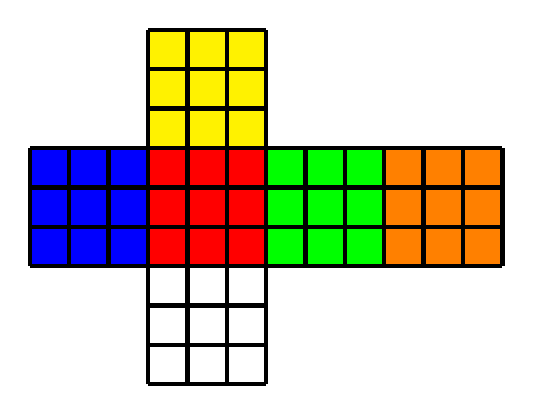
\begin{tikzpicture}[every node/.style={minimum size=0.5cm-\pgflinewidth, outer sep=0pt},scale=0.5]
    \node[fill=yellow] at (0.5,5.5) {};
    \node[fill=yellow] at (1.5,5.5) {};
    \node[fill=yellow] at (2.5,5.5) {};
    \node[fill=yellow] at (0.5,4.5) {};
    \node[fill=yellow] at (1.5,4.5) {};
    \node[fill=yellow] at (2.5,4.5) {};
    \node[fill=yellow] at (0.5,3.5) {};
    \node[fill=yellow] at (1.5,3.5) {};
    \node[fill=yellow] at (2.5,3.5) {};
    
    \node[fill=blue] at (-2.5,2.5) {};
    \node[fill=blue] at (-1.5,2.5) {};
    \node[fill=blue] at (-0.5,2.5) {};
    \node[fill=red] at (0.5,2.5) {};
    \node[fill=red] at (1.5,2.5) {};
    \node[fill=red] at (2.5,2.5) {};
    \node[fill=green] at (3.5,2.5) {};
    \node[fill=green] at (4.5,2.5) {};
    \node[fill=green] at (5.5,2.5) {};
    \node[fill=orange] at (6.5,2.5) {};
    \node[fill=orange] at (7.5,2.5) {};
    \node[fill=orange] at (8.5,2.5) {};
    
    \node[fill=blue] at (-2.5,1.5) {};
    \node[fill=blue] at (-1.5,1.5) {};
    \node[fill=blue] at (-0.5,1.5) {};
    \node[fill=red] at (0.5,1.5) {};
    \node[fill=red] at (1.5,1.5) {};
    \node[fill=red] at (2.5,1.5) {};
    \node[fill=green] at (3.5,1.5) {};
    \node[fill=green] at (4.5,1.5) {};
    \node[fill=green] at (5.5,1.5) {};
    \node[fill=orange] at (6.5,1.5) {};
    \node[fill=orange] at (7.5,1.5) {};
    \node[fill=orange] at (8.5,1.5) {};
    
    \node[fill=blue] at (-2.5,0.5) {};
    \node[fill=blue] at (-1.5,0.5) {};
    \node[fill=blue] at (-0.5,0.5) {};
    \node[fill=red] at (0.5,0.5) {};
    \node[fill=red] at (1.5,0.5) {};
    \node[fill=red] at (2.5,0.5) {};
    \node[fill=green] at (3.5,0.5) {};
    \node[fill=green] at (4.5,0.5) {};
    \node[fill=green] at (5.5,0.5) {};
    \node[fill=orange] at (6.5,0.5) {};
    \node[fill=orange] at (7.5,0.5) {};
    \node[fill=orange] at (8.5,0.5) {};
    
    \node[fill=white] at (0.5,-0.5) {};
    \node[fill=white] at (1.5,-0.5) {};
    \node[fill=white] at (2.5,-0.5) {};
    \node[fill=white] at (0.5,-1.5) {};
    \node[fill=white] at (1.5,-1.5) {};
    \node[fill=white] at (2.5,-1.5) {};
    \node[fill=white] at (0.5,-2.5) {};
    \node[fill=white] at (1.5,-2.5) {};
    \node[fill=white] at (2.5,-2.5) {};
    
    \draw[step=1cm,color=black, ultra thick] (-3,0) grid (9,3);
    \draw[step=1cm,color=black, ultra thick] (0,-3) grid (3,0);
    \draw[step=1cm,color=black, ultra thick] (0,3) grid (3,6);    
\end{tikzpicture}

\vspace{0.5cm}
\textbf{\Large{Solutions}}

Each problem has only one solution. Solution can be accessed after each problem. You can apply the scramble in the solution to your Rubik's cube with yellow on the top and red on the front.

\vspace{0.5cm}
\textbf{\Large{Acknowledgement}}

Thanks to Xi'an Jiao Tong University Rubik's Cube Club, for providing the idea of ``Cube Sudoku".

\vspace{0.5cm}
\textbf{\Large{Github link}}

\href{https://github.com/nbwzx/CubeSudoku}{https://github.com/nbwzx/CubeSudoku}

\vspace{0.5cm}
\textbf{\Large{Contributors}}

\href{https://github.com/nbwzx}{Zixing Wang}


\vspace{0.5cm}
\textbf{\Large{License}}

MIT License
\pagebreak


{\noindent\Large \textbf{No. 1\qquad Difficulty:$\bigstar$}}
\vspace{0.2cm}\\
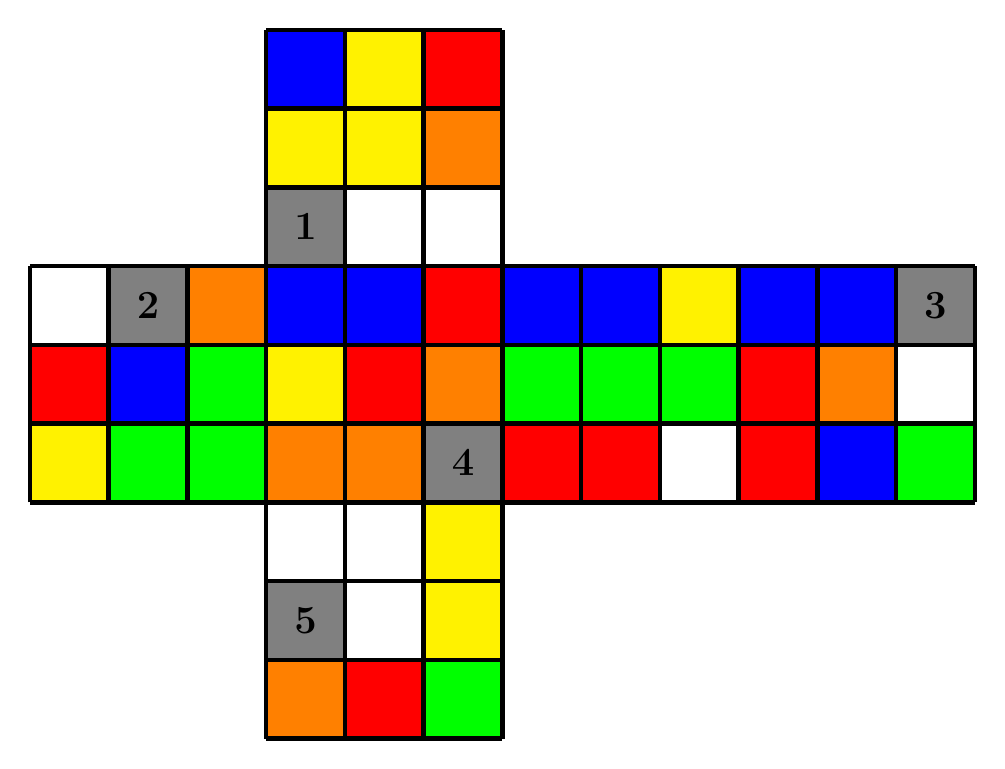
\begin{tikzpicture}[every node/.style={minimum size=1cm-\pgflinewidth, outer sep=0pt}]
\node[fill=blue] at (0.5,5.5) {};
\node[fill=yellow] at (1.5,5.5) {};
\node[fill=red] at (2.5,5.5) {};
\node[fill=yellow] at (0.5,4.5) {};
\node[fill=yellow] at (1.5,4.5) {};
\node[fill=orange] at (2.5,4.5) {};
\node[fill=gray] at (0.5,3.5) {\Large \textbf 1};
\node[fill=white] at (1.5,3.5) {};
\node[fill=white] at (2.5,3.5) {};

\node[fill=white] at (-2.5,2.5) {};
\node[fill=gray] at (-1.5,2.5) {\Large \textbf 2};
\node[fill=orange] at (-0.5,2.5) {};
\node[fill=blue] at (0.5,2.5) {};
\node[fill=blue] at (1.5,2.5) {};
\node[fill=red] at (2.5,2.5) {};
\node[fill=blue] at (3.5,2.5) {};
\node[fill=blue] at (4.5,2.5) {};
\node[fill=yellow] at (5.5,2.5) {};
\node[fill=blue] at (6.5,2.5) {};
\node[fill=blue] at (7.5,2.5) {};
\node[fill=gray] at (8.5,2.5) {\Large \textbf 3};

\node[fill=red] at (-2.5,1.5) {};
\node[fill=blue] at (-1.5,1.5) {};
\node[fill=green] at (-0.5,1.5) {};
\node[fill=yellow] at (0.5,1.5) {};
\node[fill=red] at (1.5,1.5) {};
\node[fill=orange] at (2.5,1.5) {};
\node[fill=green] at (3.5,1.5) {};
\node[fill=green] at (4.5,1.5) {};
\node[fill=green] at (5.5,1.5) {};
\node[fill=red] at (6.5,1.5) {};
\node[fill=orange] at (7.5,1.5) {};
\node[fill=white] at (8.5,1.5) {};

\node[fill=yellow] at (-2.5,0.5) {};
\node[fill=green] at (-1.5,0.5) {};
\node[fill=green] at (-0.5,0.5) {};
\node[fill=orange] at (0.5,0.5) {};
\node[fill=orange] at (1.5,0.5) {};
\node[fill=gray] at (2.5,0.5) {\Large \textbf 4};
\node[fill=red] at (3.5,0.5) {};
\node[fill=red] at (4.5,0.5) {};
\node[fill=white] at (5.5,0.5) {};
\node[fill=red] at (6.5,0.5) {};
\node[fill=blue] at (7.5,0.5) {};
\node[fill=green] at (8.5,0.5) {};

\node[fill=white] at (0.5,-0.5) {};
\node[fill=white] at (1.5,-0.5) {};
\node[fill=yellow] at (2.5,-0.5) {};
\node[fill=gray] at (0.5,-1.5) {\Large \textbf 5};
\node[fill=white] at (1.5,-1.5) {};
\node[fill=yellow] at (2.5,-1.5) {};
\node[fill=orange] at (0.5,-2.5) {};
\node[fill=red] at (1.5,-2.5) {};
\node[fill=green] at (2.5,-2.5) {};

\draw[step=1cm,color=black, ultra thick] (-3,0) grid (9,3);
\draw[step=1cm,color=black, ultra thick] (0,-3) grid (3,0);
\draw[step=1cm,color=black, ultra thick] (0,3) grid (3,6);    
\end{tikzpicture}
\vspace{0.1cm}
\\
\noindent\normalsize \newtime  \textbf{Solution 1: U2 D2 R D2 B2 D2 R D2 B2 D' B2 L U D'}
\vspace{1cm}



{\noindent\Large \textbf{No. 2\qquad Difficulty:$\bigstar$}}
\vspace{0.2cm}\\
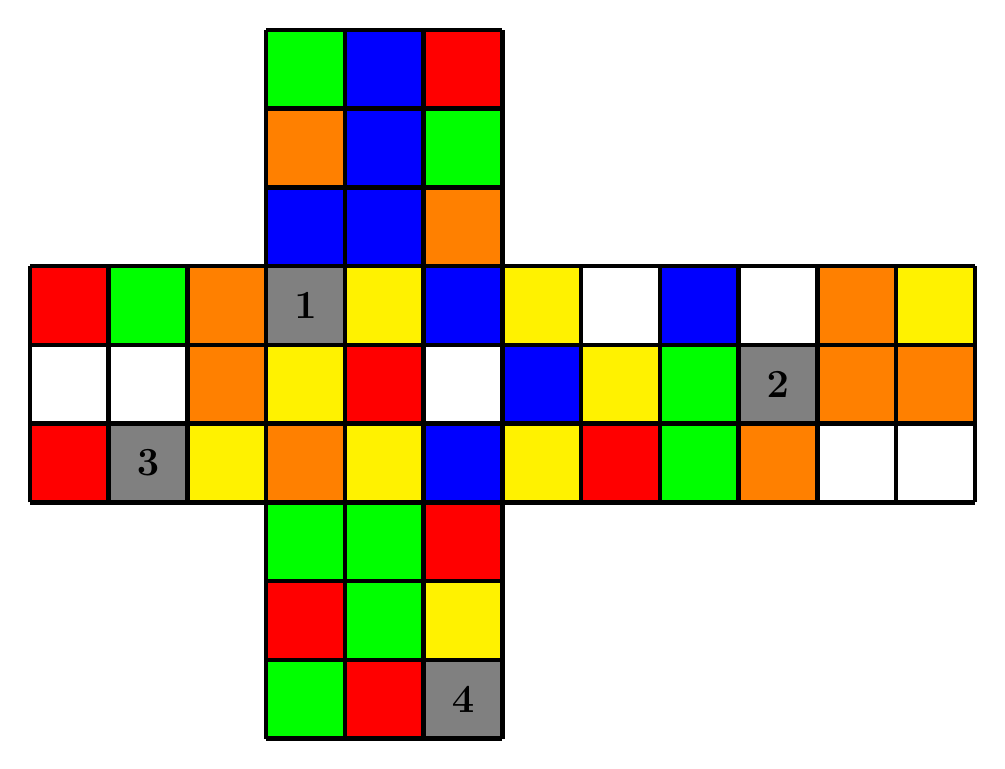
\begin{tikzpicture}[every node/.style={minimum size=1cm-\pgflinewidth, outer sep=0pt}]
\node[fill=green] at (0.5,5.5) {};
\node[fill=blue] at (1.5,5.5) {};
\node[fill=red] at (2.5,5.5) {};
\node[fill=orange] at (0.5,4.5) {};
\node[fill=blue] at (1.5,4.5) {};
\node[fill=green] at (2.5,4.5) {};
\node[fill=blue] at (0.5,3.5) {};
\node[fill=blue] at (1.5,3.5) {};
\node[fill=orange] at (2.5,3.5) {};

\node[fill=red] at (-2.5,2.5) {};
\node[fill=green] at (-1.5,2.5) {};
\node[fill=orange] at (-0.5,2.5) {};
\node[fill=gray] at (0.5,2.5) {\Large \textbf 1};
\node[fill=yellow] at (1.5,2.5) {};
\node[fill=blue] at (2.5,2.5) {};
\node[fill=yellow] at (3.5,2.5) {};
\node[fill=white] at (4.5,2.5) {};
\node[fill=blue] at (5.5,2.5) {};
\node[fill=white] at (6.5,2.5) {};
\node[fill=orange] at (7.5,2.5) {};
\node[fill=yellow] at (8.5,2.5) {};

\node[fill=white] at (-2.5,1.5) {};
\node[fill=white] at (-1.5,1.5) {};
\node[fill=orange] at (-0.5,1.5) {};
\node[fill=yellow] at (0.5,1.5) {};
\node[fill=red] at (1.5,1.5) {};
\node[fill=white] at (2.5,1.5) {};
\node[fill=blue] at (3.5,1.5) {};
\node[fill=yellow] at (4.5,1.5) {};
\node[fill=green] at (5.5,1.5) {};
\node[fill=gray] at (6.5,1.5) {\Large \textbf 2};
\node[fill=orange] at (7.5,1.5) {};
\node[fill=orange] at (8.5,1.5) {};

\node[fill=red] at (-2.5,0.5) {};
\node[fill=gray] at (-1.5,0.5) {\Large \textbf 3};
\node[fill=yellow] at (-0.5,0.5) {};
\node[fill=orange] at (0.5,0.5) {};
\node[fill=yellow] at (1.5,0.5) {};
\node[fill=blue] at (2.5,0.5) {};
\node[fill=yellow] at (3.5,0.5) {};
\node[fill=red] at (4.5,0.5) {};
\node[fill=green] at (5.5,0.5) {};
\node[fill=orange] at (6.5,0.5) {};
\node[fill=white] at (7.5,0.5) {};
\node[fill=white] at (8.5,0.5) {};

\node[fill=green] at (0.5,-0.5) {};
\node[fill=green] at (1.5,-0.5) {};
\node[fill=red] at (2.5,-0.5) {};
\node[fill=red] at (0.5,-1.5) {};
\node[fill=green] at (1.5,-1.5) {};
\node[fill=yellow] at (2.5,-1.5) {};
\node[fill=green] at (0.5,-2.5) {};
\node[fill=red] at (1.5,-2.5) {};
\node[fill=gray] at (2.5,-2.5) {\Large \textbf 4};

\draw[step=1cm,color=black, ultra thick] (-3,0) grid (9,3);
\draw[step=1cm,color=black, ultra thick] (0,-3) grid (3,0);
\draw[step=1cm,color=black, ultra thick] (0,3) grid (3,6);    
\end{tikzpicture}
\vspace{0.1cm}
\\
\noindent\normalsize \newtime  \textbf{Solution 2: R D2 F D2 B L2 B U2 F U2 R2 B2 R2 L' F' L2 B R F D' Fw}
\vspace{1cm}



{\noindent\Large \textbf{No. 3\qquad Difficulty:$\bigstar$}}
\vspace{0.2cm}\\
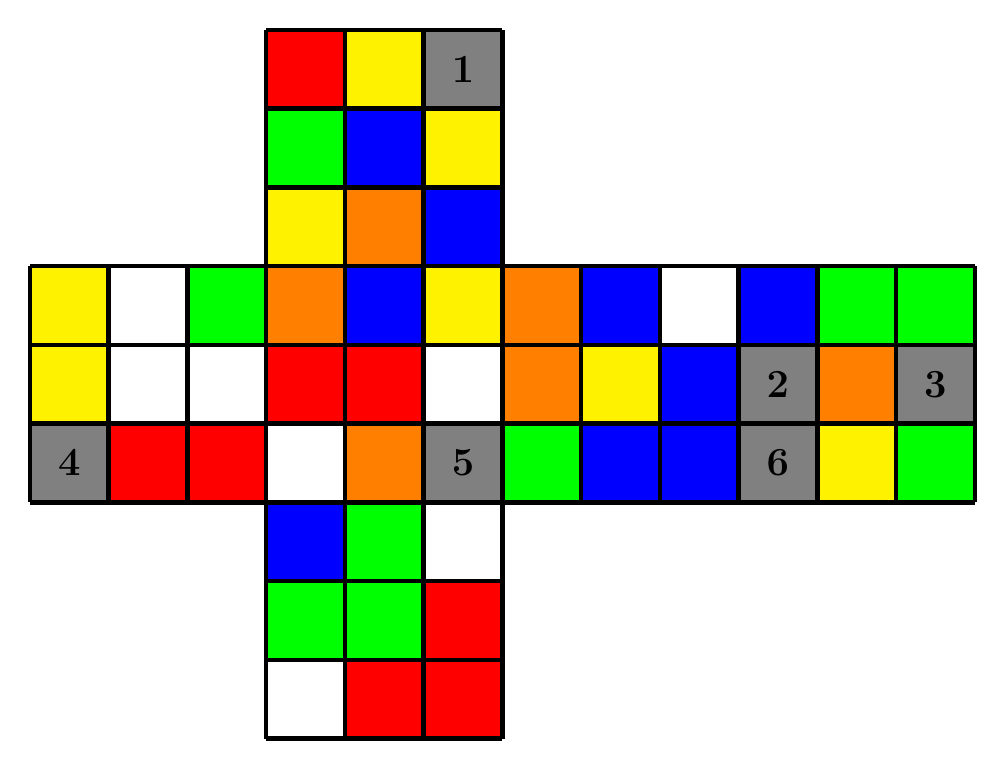
\begin{tikzpicture}[every node/.style={minimum size=1cm-\pgflinewidth, outer sep=0pt}]
\node[fill=red] at (0.5,5.5) {};
\node[fill=yellow] at (1.5,5.5) {};
\node[fill=gray] at (2.5,5.5) {\Large \textbf 1};
\node[fill=green] at (0.5,4.5) {};
\node[fill=blue] at (1.5,4.5) {};
\node[fill=yellow] at (2.5,4.5) {};
\node[fill=yellow] at (0.5,3.5) {};
\node[fill=orange] at (1.5,3.5) {};
\node[fill=blue] at (2.5,3.5) {};

\node[fill=yellow] at (-2.5,2.5) {};
\node[fill=white] at (-1.5,2.5) {};
\node[fill=green] at (-0.5,2.5) {};
\node[fill=orange] at (0.5,2.5) {};
\node[fill=blue] at (1.5,2.5) {};
\node[fill=yellow] at (2.5,2.5) {};
\node[fill=orange] at (3.5,2.5) {};
\node[fill=blue] at (4.5,2.5) {};
\node[fill=white] at (5.5,2.5) {};
\node[fill=blue] at (6.5,2.5) {};
\node[fill=green] at (7.5,2.5) {};
\node[fill=green] at (8.5,2.5) {};

\node[fill=yellow] at (-2.5,1.5) {};
\node[fill=white] at (-1.5,1.5) {};
\node[fill=white] at (-0.5,1.5) {};
\node[fill=red] at (0.5,1.5) {};
\node[fill=red] at (1.5,1.5) {};
\node[fill=white] at (2.5,1.5) {};
\node[fill=orange] at (3.5,1.5) {};
\node[fill=yellow] at (4.5,1.5) {};
\node[fill=blue] at (5.5,1.5) {};
\node[fill=gray] at (6.5,1.5) {\Large \textbf 2};
\node[fill=orange] at (7.5,1.5) {};
\node[fill=gray] at (8.5,1.5) {\Large \textbf 3};

\node[fill=gray] at (-2.5,0.5) {\Large \textbf 4};
\node[fill=red] at (-1.5,0.5) {};
\node[fill=red] at (-0.5,0.5) {};
\node[fill=white] at (0.5,0.5) {};
\node[fill=orange] at (1.5,0.5) {};
\node[fill=gray] at (2.5,0.5) {\Large \textbf 5};
\node[fill=green] at (3.5,0.5) {};
\node[fill=blue] at (4.5,0.5) {};
\node[fill=blue] at (5.5,0.5) {};
\node[fill=gray] at (6.5,0.5) {\Large \textbf 6};
\node[fill=yellow] at (7.5,0.5) {};
\node[fill=green] at (8.5,0.5) {};

\node[fill=blue] at (0.5,-0.5) {};
\node[fill=green] at (1.5,-0.5) {};
\node[fill=white] at (2.5,-0.5) {};
\node[fill=green] at (0.5,-1.5) {};
\node[fill=green] at (1.5,-1.5) {};
\node[fill=red] at (2.5,-1.5) {};
\node[fill=white] at (0.5,-2.5) {};
\node[fill=red] at (1.5,-2.5) {};
\node[fill=red] at (2.5,-2.5) {};

\draw[step=1cm,color=black, ultra thick] (-3,0) grid (9,3);
\draw[step=1cm,color=black, ultra thick] (0,-3) grid (3,0);
\draw[step=1cm,color=black, ultra thick] (0,3) grid (3,6);    
\end{tikzpicture}
\vspace{0.1cm}
\\
\noindent\normalsize \newtime  \textbf{Solution 3: B2 L' U2 L' D2 B2 U2 L' D2 B2 L R B' R' B2 D R' B' F2 U L2 Fw}
\vspace{1cm}



{\noindent\Large \textbf{No. 4\qquad Difficulty:$\bigstar$}}
\vspace{0.2cm}\\
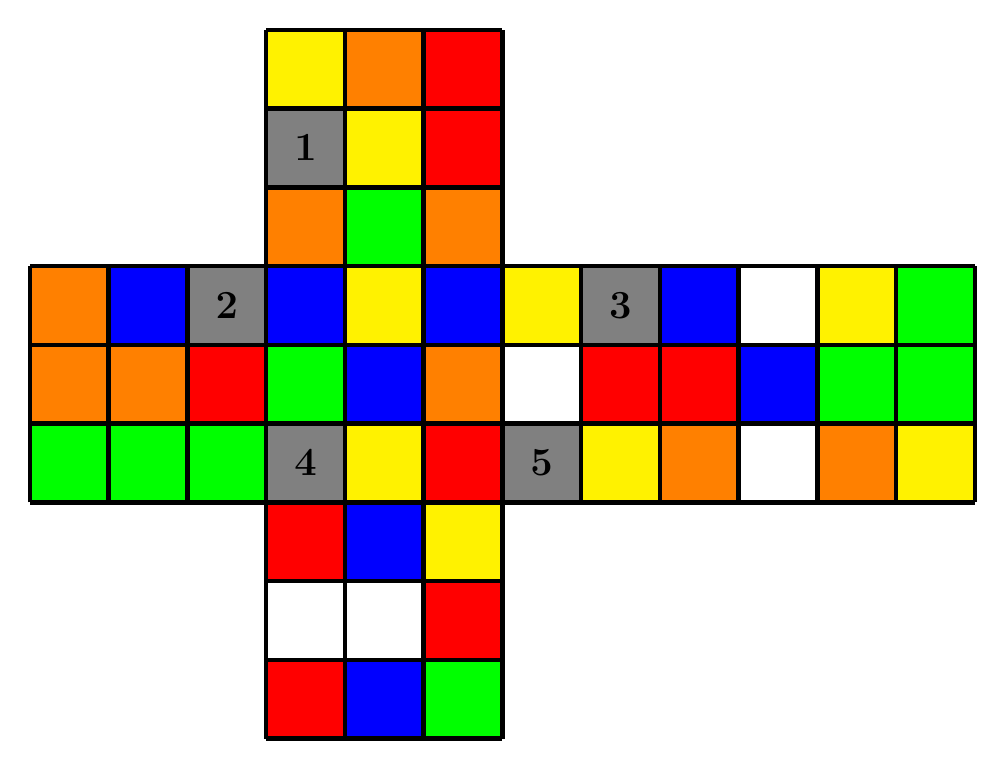
\begin{tikzpicture}[every node/.style={minimum size=1cm-\pgflinewidth, outer sep=0pt}]
\node[fill=yellow] at (0.5,5.5) {};
\node[fill=orange] at (1.5,5.5) {};
\node[fill=red] at (2.5,5.5) {};
\node[fill=gray] at (0.5,4.5) {\Large \textbf 1};
\node[fill=yellow] at (1.5,4.5) {};
\node[fill=red] at (2.5,4.5) {};
\node[fill=orange] at (0.5,3.5) {};
\node[fill=green] at (1.5,3.5) {};
\node[fill=orange] at (2.5,3.5) {};

\node[fill=orange] at (-2.5,2.5) {};
\node[fill=blue] at (-1.5,2.5) {};
\node[fill=gray] at (-0.5,2.5) {\Large \textbf 2};
\node[fill=blue] at (0.5,2.5) {};
\node[fill=yellow] at (1.5,2.5) {};
\node[fill=blue] at (2.5,2.5) {};
\node[fill=yellow] at (3.5,2.5) {};
\node[fill=gray] at (4.5,2.5) {\Large \textbf 3};
\node[fill=blue] at (5.5,2.5) {};
\node[fill=white] at (6.5,2.5) {};
\node[fill=yellow] at (7.5,2.5) {};
\node[fill=green] at (8.5,2.5) {};

\node[fill=orange] at (-2.5,1.5) {};
\node[fill=orange] at (-1.5,1.5) {};
\node[fill=red] at (-0.5,1.5) {};
\node[fill=green] at (0.5,1.5) {};
\node[fill=blue] at (1.5,1.5) {};
\node[fill=orange] at (2.5,1.5) {};
\node[fill=white] at (3.5,1.5) {};
\node[fill=red] at (4.5,1.5) {};
\node[fill=red] at (5.5,1.5) {};
\node[fill=blue] at (6.5,1.5) {};
\node[fill=green] at (7.5,1.5) {};
\node[fill=green] at (8.5,1.5) {};

\node[fill=green] at (-2.5,0.5) {};
\node[fill=green] at (-1.5,0.5) {};
\node[fill=green] at (-0.5,0.5) {};
\node[fill=gray] at (0.5,0.5) {\Large \textbf 4};
\node[fill=yellow] at (1.5,0.5) {};
\node[fill=red] at (2.5,0.5) {};
\node[fill=gray] at (3.5,0.5) {\Large \textbf 5};
\node[fill=yellow] at (4.5,0.5) {};
\node[fill=orange] at (5.5,0.5) {};
\node[fill=white] at (6.5,0.5) {};
\node[fill=orange] at (7.5,0.5) {};
\node[fill=yellow] at (8.5,0.5) {};

\node[fill=red] at (0.5,-0.5) {};
\node[fill=blue] at (1.5,-0.5) {};
\node[fill=yellow] at (2.5,-0.5) {};
\node[fill=white] at (0.5,-1.5) {};
\node[fill=white] at (1.5,-1.5) {};
\node[fill=red] at (2.5,-1.5) {};
\node[fill=red] at (0.5,-2.5) {};
\node[fill=blue] at (1.5,-2.5) {};
\node[fill=green] at (2.5,-2.5) {};

\draw[step=1cm,color=black, ultra thick] (-3,0) grid (9,3);
\draw[step=1cm,color=black, ultra thick] (0,-3) grid (3,0);
\draw[step=1cm,color=black, ultra thick] (0,3) grid (3,6);    
\end{tikzpicture}
\vspace{0.1cm}
\\
\noindent\normalsize \newtime  \textbf{Solution 4: B2 U L2 F2 D2 L2 F2 U' R2 U B2 D' F R B2 L D2 L2 F L' R2 Uw'}
\vspace{1cm}



{\noindent\Large \textbf{No. 5\qquad Difficulty:$\bigstar$}}
\vspace{0.2cm}\\
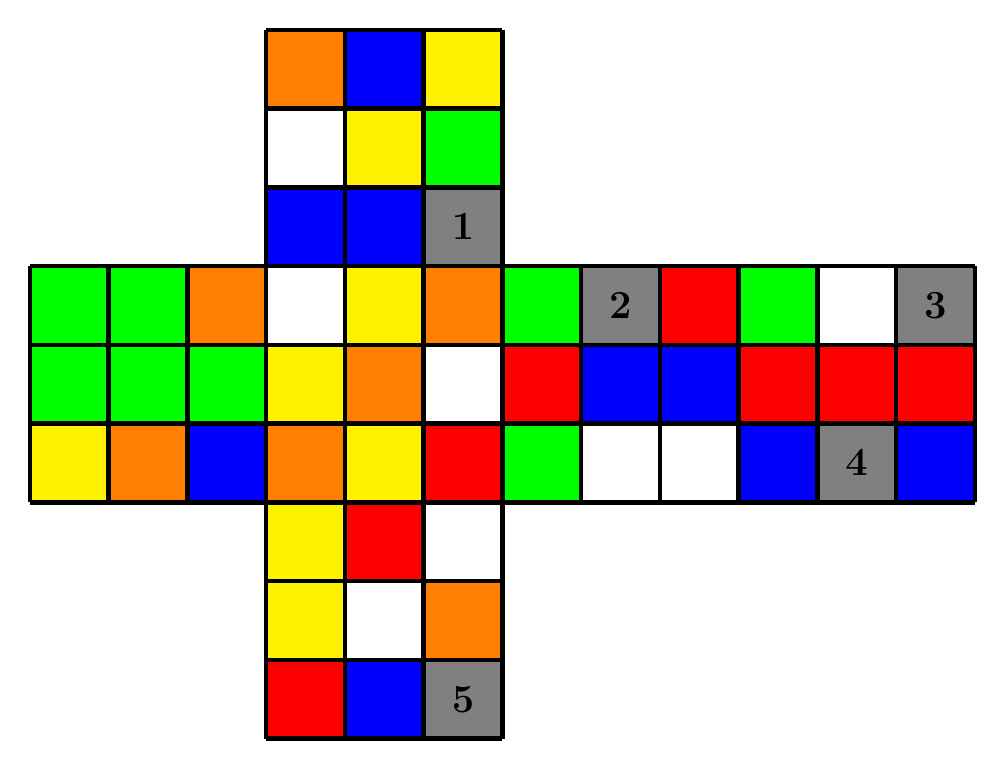
\begin{tikzpicture}[every node/.style={minimum size=1cm-\pgflinewidth, outer sep=0pt}]
\node[fill=orange] at (0.5,5.5) {};
\node[fill=blue] at (1.5,5.5) {};
\node[fill=yellow] at (2.5,5.5) {};
\node[fill=white] at (0.5,4.5) {};
\node[fill=yellow] at (1.5,4.5) {};
\node[fill=green] at (2.5,4.5) {};
\node[fill=blue] at (0.5,3.5) {};
\node[fill=blue] at (1.5,3.5) {};
\node[fill=gray] at (2.5,3.5) {\Large \textbf 1};

\node[fill=green] at (-2.5,2.5) {};
\node[fill=green] at (-1.5,2.5) {};
\node[fill=orange] at (-0.5,2.5) {};
\node[fill=white] at (0.5,2.5) {};
\node[fill=yellow] at (1.5,2.5) {};
\node[fill=orange] at (2.5,2.5) {};
\node[fill=green] at (3.5,2.5) {};
\node[fill=gray] at (4.5,2.5) {\Large \textbf 2};
\node[fill=red] at (5.5,2.5) {};
\node[fill=green] at (6.5,2.5) {};
\node[fill=white] at (7.5,2.5) {};
\node[fill=gray] at (8.5,2.5) {\Large \textbf 3};

\node[fill=green] at (-2.5,1.5) {};
\node[fill=green] at (-1.5,1.5) {};
\node[fill=green] at (-0.5,1.5) {};
\node[fill=yellow] at (0.5,1.5) {};
\node[fill=orange] at (1.5,1.5) {};
\node[fill=white] at (2.5,1.5) {};
\node[fill=red] at (3.5,1.5) {};
\node[fill=blue] at (4.5,1.5) {};
\node[fill=blue] at (5.5,1.5) {};
\node[fill=red] at (6.5,1.5) {};
\node[fill=red] at (7.5,1.5) {};
\node[fill=red] at (8.5,1.5) {};

\node[fill=yellow] at (-2.5,0.5) {};
\node[fill=orange] at (-1.5,0.5) {};
\node[fill=blue] at (-0.5,0.5) {};
\node[fill=orange] at (0.5,0.5) {};
\node[fill=yellow] at (1.5,0.5) {};
\node[fill=red] at (2.5,0.5) {};
\node[fill=green] at (3.5,0.5) {};
\node[fill=white] at (4.5,0.5) {};
\node[fill=white] at (5.5,0.5) {};
\node[fill=blue] at (6.5,0.5) {};
\node[fill=gray] at (7.5,0.5) {\Large \textbf 4};
\node[fill=blue] at (8.5,0.5) {};

\node[fill=yellow] at (0.5,-0.5) {};
\node[fill=red] at (1.5,-0.5) {};
\node[fill=white] at (2.5,-0.5) {};
\node[fill=yellow] at (0.5,-1.5) {};
\node[fill=white] at (1.5,-1.5) {};
\node[fill=orange] at (2.5,-1.5) {};
\node[fill=red] at (0.5,-2.5) {};
\node[fill=blue] at (1.5,-2.5) {};
\node[fill=gray] at (2.5,-2.5) {\Large \textbf 5};

\draw[step=1cm,color=black, ultra thick] (-3,0) grid (9,3);
\draw[step=1cm,color=black, ultra thick] (0,-3) grid (3,0);
\draw[step=1cm,color=black, ultra thick] (0,3) grid (3,6);    
\end{tikzpicture}
\vspace{0.1cm}
\\
\noindent\normalsize \newtime  \textbf{Solution 5: R2 B2 D2 R2 F2 U' L2 D B2 L2 D2 F' L' F' R2 F D2 R2 F' R' U Uw2}
\vspace{1cm}



{\noindent\Large \textbf{No. 6\qquad Difficulty:$\bigstar$}}
\vspace{0.2cm}\\
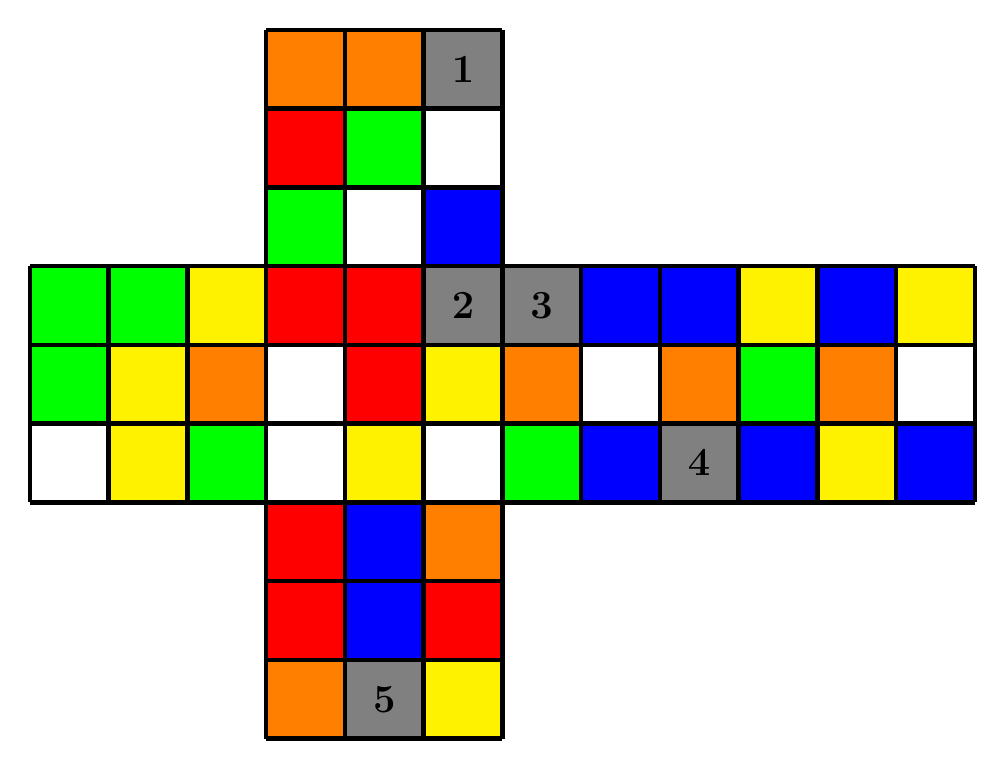
\begin{tikzpicture}[every node/.style={minimum size=1cm-\pgflinewidth, outer sep=0pt}]
\node[fill=orange] at (0.5,5.5) {};
\node[fill=orange] at (1.5,5.5) {};
\node[fill=gray] at (2.5,5.5) {\Large \textbf 1};
\node[fill=red] at (0.5,4.5) {};
\node[fill=green] at (1.5,4.5) {};
\node[fill=white] at (2.5,4.5) {};
\node[fill=green] at (0.5,3.5) {};
\node[fill=white] at (1.5,3.5) {};
\node[fill=blue] at (2.5,3.5) {};

\node[fill=green] at (-2.5,2.5) {};
\node[fill=green] at (-1.5,2.5) {};
\node[fill=yellow] at (-0.5,2.5) {};
\node[fill=red] at (0.5,2.5) {};
\node[fill=red] at (1.5,2.5) {};
\node[fill=gray] at (2.5,2.5) {\Large \textbf 2};
\node[fill=gray] at (3.5,2.5) {\Large \textbf 3};
\node[fill=blue] at (4.5,2.5) {};
\node[fill=blue] at (5.5,2.5) {};
\node[fill=yellow] at (6.5,2.5) {};
\node[fill=blue] at (7.5,2.5) {};
\node[fill=yellow] at (8.5,2.5) {};

\node[fill=green] at (-2.5,1.5) {};
\node[fill=yellow] at (-1.5,1.5) {};
\node[fill=orange] at (-0.5,1.5) {};
\node[fill=white] at (0.5,1.5) {};
\node[fill=red] at (1.5,1.5) {};
\node[fill=yellow] at (2.5,1.5) {};
\node[fill=orange] at (3.5,1.5) {};
\node[fill=white] at (4.5,1.5) {};
\node[fill=orange] at (5.5,1.5) {};
\node[fill=green] at (6.5,1.5) {};
\node[fill=orange] at (7.5,1.5) {};
\node[fill=white] at (8.5,1.5) {};

\node[fill=white] at (-2.5,0.5) {};
\node[fill=yellow] at (-1.5,0.5) {};
\node[fill=green] at (-0.5,0.5) {};
\node[fill=white] at (0.5,0.5) {};
\node[fill=yellow] at (1.5,0.5) {};
\node[fill=white] at (2.5,0.5) {};
\node[fill=green] at (3.5,0.5) {};
\node[fill=blue] at (4.5,0.5) {};
\node[fill=gray] at (5.5,0.5) {\Large \textbf 4};
\node[fill=blue] at (6.5,0.5) {};
\node[fill=yellow] at (7.5,0.5) {};
\node[fill=blue] at (8.5,0.5) {};

\node[fill=red] at (0.5,-0.5) {};
\node[fill=blue] at (1.5,-0.5) {};
\node[fill=orange] at (2.5,-0.5) {};
\node[fill=red] at (0.5,-1.5) {};
\node[fill=blue] at (1.5,-1.5) {};
\node[fill=red] at (2.5,-1.5) {};
\node[fill=orange] at (0.5,-2.5) {};
\node[fill=gray] at (1.5,-2.5) {\Large \textbf 5};
\node[fill=yellow] at (2.5,-2.5) {};

\draw[step=1cm,color=black, ultra thick] (-3,0) grid (9,3);
\draw[step=1cm,color=black, ultra thick] (0,-3) grid (3,0);
\draw[step=1cm,color=black, ultra thick] (0,3) grid (3,6);    
\end{tikzpicture}
\vspace{0.1cm}
\\
\noindent\normalsize \newtime  \textbf{Solution 6: F2 R2 F' R2 F2 R2 F' R2 B L2 F2 R B R2 F2 L' B D' B U Fw'}
\vspace{1cm}



{\noindent\Large \textbf{No. 7\qquad Difficulty:$\bigstar$}}
\vspace{0.2cm}\\
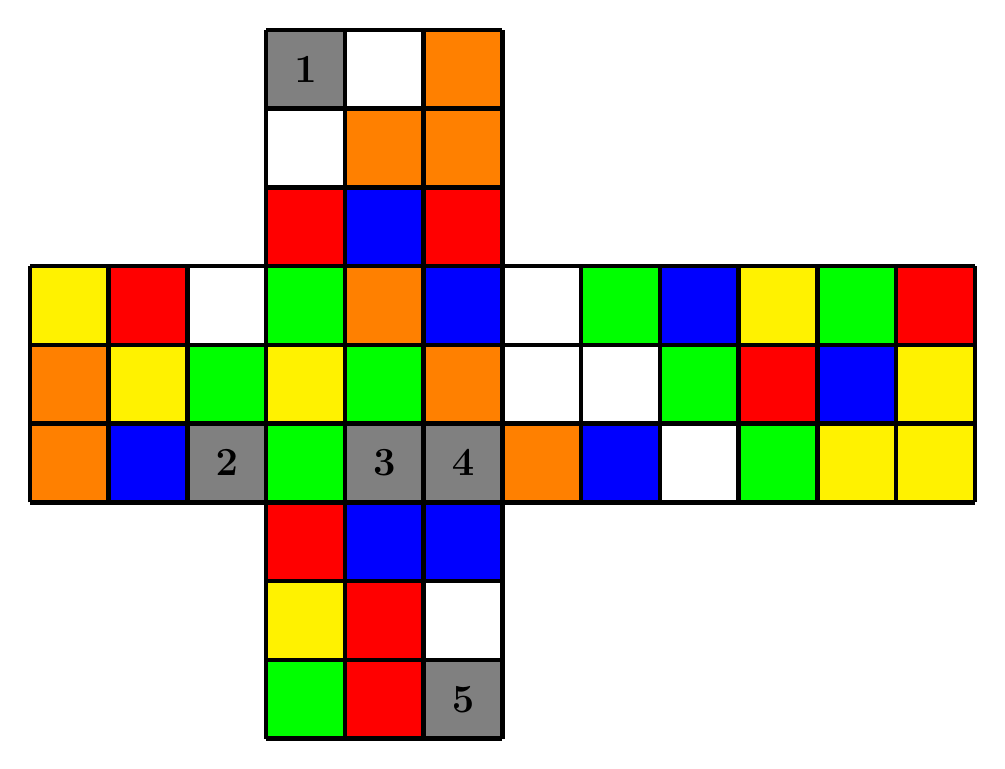
\begin{tikzpicture}[every node/.style={minimum size=1cm-\pgflinewidth, outer sep=0pt}]
\node[fill=gray] at (0.5,5.5) {\Large \textbf 1};
\node[fill=white] at (1.5,5.5) {};
\node[fill=orange] at (2.5,5.5) {};
\node[fill=white] at (0.5,4.5) {};
\node[fill=orange] at (1.5,4.5) {};
\node[fill=orange] at (2.5,4.5) {};
\node[fill=red] at (0.5,3.5) {};
\node[fill=blue] at (1.5,3.5) {};
\node[fill=red] at (2.5,3.5) {};

\node[fill=yellow] at (-2.5,2.5) {};
\node[fill=red] at (-1.5,2.5) {};
\node[fill=white] at (-0.5,2.5) {};
\node[fill=green] at (0.5,2.5) {};
\node[fill=orange] at (1.5,2.5) {};
\node[fill=blue] at (2.5,2.5) {};
\node[fill=white] at (3.5,2.5) {};
\node[fill=green] at (4.5,2.5) {};
\node[fill=blue] at (5.5,2.5) {};
\node[fill=yellow] at (6.5,2.5) {};
\node[fill=green] at (7.5,2.5) {};
\node[fill=red] at (8.5,2.5) {};

\node[fill=orange] at (-2.5,1.5) {};
\node[fill=yellow] at (-1.5,1.5) {};
\node[fill=green] at (-0.5,1.5) {};
\node[fill=yellow] at (0.5,1.5) {};
\node[fill=green] at (1.5,1.5) {};
\node[fill=orange] at (2.5,1.5) {};
\node[fill=white] at (3.5,1.5) {};
\node[fill=white] at (4.5,1.5) {};
\node[fill=green] at (5.5,1.5) {};
\node[fill=red] at (6.5,1.5) {};
\node[fill=blue] at (7.5,1.5) {};
\node[fill=yellow] at (8.5,1.5) {};

\node[fill=orange] at (-2.5,0.5) {};
\node[fill=blue] at (-1.5,0.5) {};
\node[fill=gray] at (-0.5,0.5) {\Large \textbf 2};
\node[fill=green] at (0.5,0.5) {};
\node[fill=gray] at (1.5,0.5) {\Large \textbf 3};
\node[fill=gray] at (2.5,0.5) {\Large \textbf 4};
\node[fill=orange] at (3.5,0.5) {};
\node[fill=blue] at (4.5,0.5) {};
\node[fill=white] at (5.5,0.5) {};
\node[fill=green] at (6.5,0.5) {};
\node[fill=yellow] at (7.5,0.5) {};
\node[fill=yellow] at (8.5,0.5) {};

\node[fill=red] at (0.5,-0.5) {};
\node[fill=blue] at (1.5,-0.5) {};
\node[fill=blue] at (2.5,-0.5) {};
\node[fill=yellow] at (0.5,-1.5) {};
\node[fill=red] at (1.5,-1.5) {};
\node[fill=white] at (2.5,-1.5) {};
\node[fill=green] at (0.5,-2.5) {};
\node[fill=red] at (1.5,-2.5) {};
\node[fill=gray] at (2.5,-2.5) {\Large \textbf 5};

\draw[step=1cm,color=black, ultra thick] (-3,0) grid (9,3);
\draw[step=1cm,color=black, ultra thick] (0,-3) grid (3,0);
\draw[step=1cm,color=black, ultra thick] (0,3) grid (3,6);    
\end{tikzpicture}
\vspace{0.1cm}
\\
\noindent\normalsize \newtime  \textbf{Solution 7: F' U' R2 B2 U L2 F2 L2 D R2 U' R2 B R U B D F' L2 B' R Rw' Uw}
\vspace{1cm}



{\noindent\Large \textbf{No. 8\qquad Difficulty:$\bigstar$}}
\vspace{0.2cm}\\
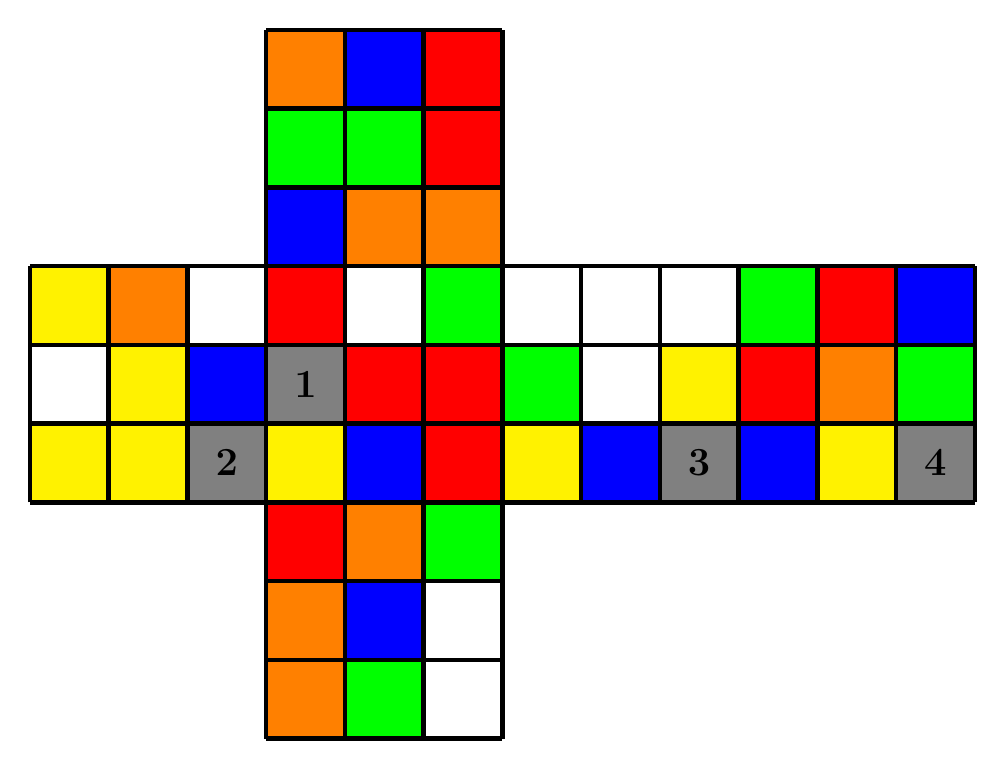
\begin{tikzpicture}[every node/.style={minimum size=1cm-\pgflinewidth, outer sep=0pt}]
\node[fill=orange] at (0.5,5.5) {};
\node[fill=blue] at (1.5,5.5) {};
\node[fill=red] at (2.5,5.5) {};
\node[fill=green] at (0.5,4.5) {};
\node[fill=green] at (1.5,4.5) {};
\node[fill=red] at (2.5,4.5) {};
\node[fill=blue] at (0.5,3.5) {};
\node[fill=orange] at (1.5,3.5) {};
\node[fill=orange] at (2.5,3.5) {};

\node[fill=yellow] at (-2.5,2.5) {};
\node[fill=orange] at (-1.5,2.5) {};
\node[fill=white] at (-0.5,2.5) {};
\node[fill=red] at (0.5,2.5) {};
\node[fill=white] at (1.5,2.5) {};
\node[fill=green] at (2.5,2.5) {};
\node[fill=white] at (3.5,2.5) {};
\node[fill=white] at (4.5,2.5) {};
\node[fill=white] at (5.5,2.5) {};
\node[fill=green] at (6.5,2.5) {};
\node[fill=red] at (7.5,2.5) {};
\node[fill=blue] at (8.5,2.5) {};

\node[fill=white] at (-2.5,1.5) {};
\node[fill=yellow] at (-1.5,1.5) {};
\node[fill=blue] at (-0.5,1.5) {};
\node[fill=gray] at (0.5,1.5) {\Large \textbf 1};
\node[fill=red] at (1.5,1.5) {};
\node[fill=red] at (2.5,1.5) {};
\node[fill=green] at (3.5,1.5) {};
\node[fill=white] at (4.5,1.5) {};
\node[fill=yellow] at (5.5,1.5) {};
\node[fill=red] at (6.5,1.5) {};
\node[fill=orange] at (7.5,1.5) {};
\node[fill=green] at (8.5,1.5) {};

\node[fill=yellow] at (-2.5,0.5) {};
\node[fill=yellow] at (-1.5,0.5) {};
\node[fill=gray] at (-0.5,0.5) {\Large \textbf 2};
\node[fill=yellow] at (0.5,0.5) {};
\node[fill=blue] at (1.5,0.5) {};
\node[fill=red] at (2.5,0.5) {};
\node[fill=yellow] at (3.5,0.5) {};
\node[fill=blue] at (4.5,0.5) {};
\node[fill=gray] at (5.5,0.5) {\Large \textbf 3};
\node[fill=blue] at (6.5,0.5) {};
\node[fill=yellow] at (7.5,0.5) {};
\node[fill=gray] at (8.5,0.5) {\Large \textbf 4};

\node[fill=red] at (0.5,-0.5) {};
\node[fill=orange] at (1.5,-0.5) {};
\node[fill=green] at (2.5,-0.5) {};
\node[fill=orange] at (0.5,-1.5) {};
\node[fill=blue] at (1.5,-1.5) {};
\node[fill=white] at (2.5,-1.5) {};
\node[fill=orange] at (0.5,-2.5) {};
\node[fill=green] at (1.5,-2.5) {};
\node[fill=white] at (2.5,-2.5) {};

\draw[step=1cm,color=black, ultra thick] (-3,0) grid (9,3);
\draw[step=1cm,color=black, ultra thick] (0,-3) grid (3,0);
\draw[step=1cm,color=black, ultra thick] (0,3) grid (3,6);    
\end{tikzpicture}
\vspace{0.1cm}
\\
\noindent\normalsize \newtime  \textbf{Solution 8: D R2 U2 F' L2 F' L2 B2 L2 D2 B F' D2 R' U F2 U R2 F R D2 Fw'}
\vspace{1cm}



{\noindent\Large \textbf{No. 9\qquad Difficulty:$\bigstar$}}
\vspace{0.2cm}\\
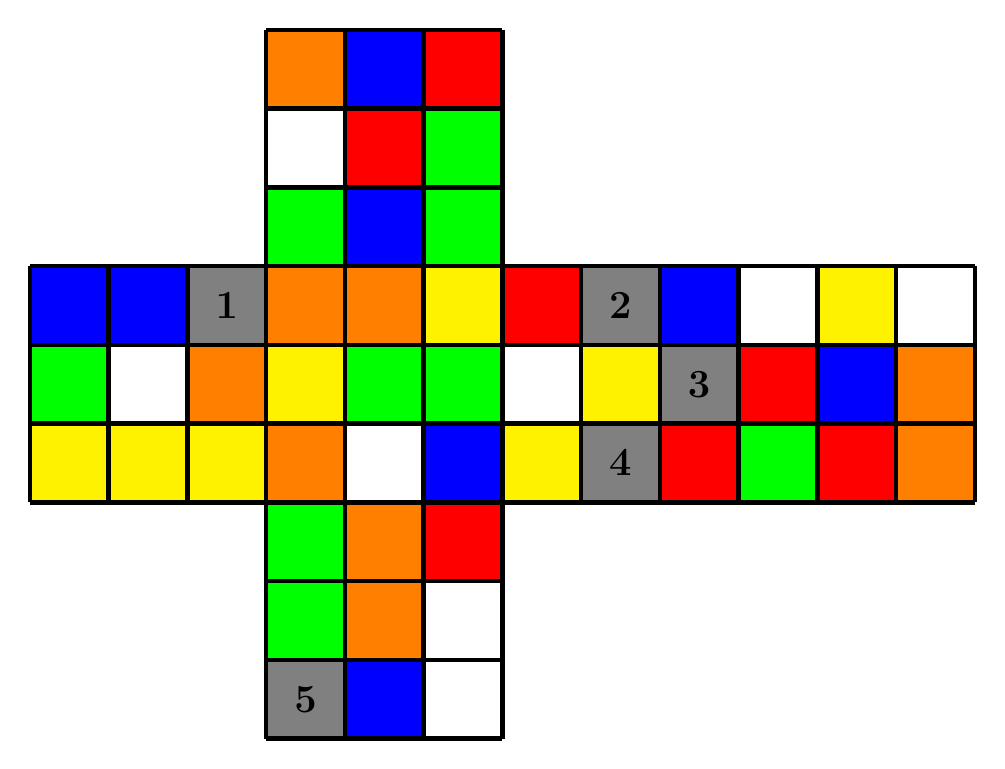
\begin{tikzpicture}[every node/.style={minimum size=1cm-\pgflinewidth, outer sep=0pt}]
\node[fill=orange] at (0.5,5.5) {};
\node[fill=blue] at (1.5,5.5) {};
\node[fill=red] at (2.5,5.5) {};
\node[fill=white] at (0.5,4.5) {};
\node[fill=red] at (1.5,4.5) {};
\node[fill=green] at (2.5,4.5) {};
\node[fill=green] at (0.5,3.5) {};
\node[fill=blue] at (1.5,3.5) {};
\node[fill=green] at (2.5,3.5) {};

\node[fill=blue] at (-2.5,2.5) {};
\node[fill=blue] at (-1.5,2.5) {};
\node[fill=gray] at (-0.5,2.5) {\Large \textbf 1};
\node[fill=orange] at (0.5,2.5) {};
\node[fill=orange] at (1.5,2.5) {};
\node[fill=yellow] at (2.5,2.5) {};
\node[fill=red] at (3.5,2.5) {};
\node[fill=gray] at (4.5,2.5) {\Large \textbf 2};
\node[fill=blue] at (5.5,2.5) {};
\node[fill=white] at (6.5,2.5) {};
\node[fill=yellow] at (7.5,2.5) {};
\node[fill=white] at (8.5,2.5) {};

\node[fill=green] at (-2.5,1.5) {};
\node[fill=white] at (-1.5,1.5) {};
\node[fill=orange] at (-0.5,1.5) {};
\node[fill=yellow] at (0.5,1.5) {};
\node[fill=green] at (1.5,1.5) {};
\node[fill=green] at (2.5,1.5) {};
\node[fill=white] at (3.5,1.5) {};
\node[fill=yellow] at (4.5,1.5) {};
\node[fill=gray] at (5.5,1.5) {\Large \textbf 3};
\node[fill=red] at (6.5,1.5) {};
\node[fill=blue] at (7.5,1.5) {};
\node[fill=orange] at (8.5,1.5) {};

\node[fill=yellow] at (-2.5,0.5) {};
\node[fill=yellow] at (-1.5,0.5) {};
\node[fill=yellow] at (-0.5,0.5) {};
\node[fill=orange] at (0.5,0.5) {};
\node[fill=white] at (1.5,0.5) {};
\node[fill=blue] at (2.5,0.5) {};
\node[fill=yellow] at (3.5,0.5) {};
\node[fill=gray] at (4.5,0.5) {\Large \textbf 4};
\node[fill=red] at (5.5,0.5) {};
\node[fill=green] at (6.5,0.5) {};
\node[fill=red] at (7.5,0.5) {};
\node[fill=orange] at (8.5,0.5) {};

\node[fill=green] at (0.5,-0.5) {};
\node[fill=orange] at (1.5,-0.5) {};
\node[fill=red] at (2.5,-0.5) {};
\node[fill=green] at (0.5,-1.5) {};
\node[fill=orange] at (1.5,-1.5) {};
\node[fill=white] at (2.5,-1.5) {};
\node[fill=gray] at (0.5,-2.5) {\Large \textbf 5};
\node[fill=blue] at (1.5,-2.5) {};
\node[fill=white] at (2.5,-2.5) {};

\draw[step=1cm,color=black, ultra thick] (-3,0) grid (9,3);
\draw[step=1cm,color=black, ultra thick] (0,-3) grid (3,0);
\draw[step=1cm,color=black, ultra thick] (0,3) grid (3,6);    
\end{tikzpicture}
\vspace{0.1cm}
\\
\noindent\normalsize \newtime  \textbf{Solution 9: B' R U R L D B2 L' B R2 U2 R F2 L F2 U2 R2 B2 D2 R2 B2 Rw Uw}
\vspace{1cm}



{\noindent\Large \textbf{No. 10\qquad Difficulty:$\bigstar$}}
\vspace{0.2cm}\\
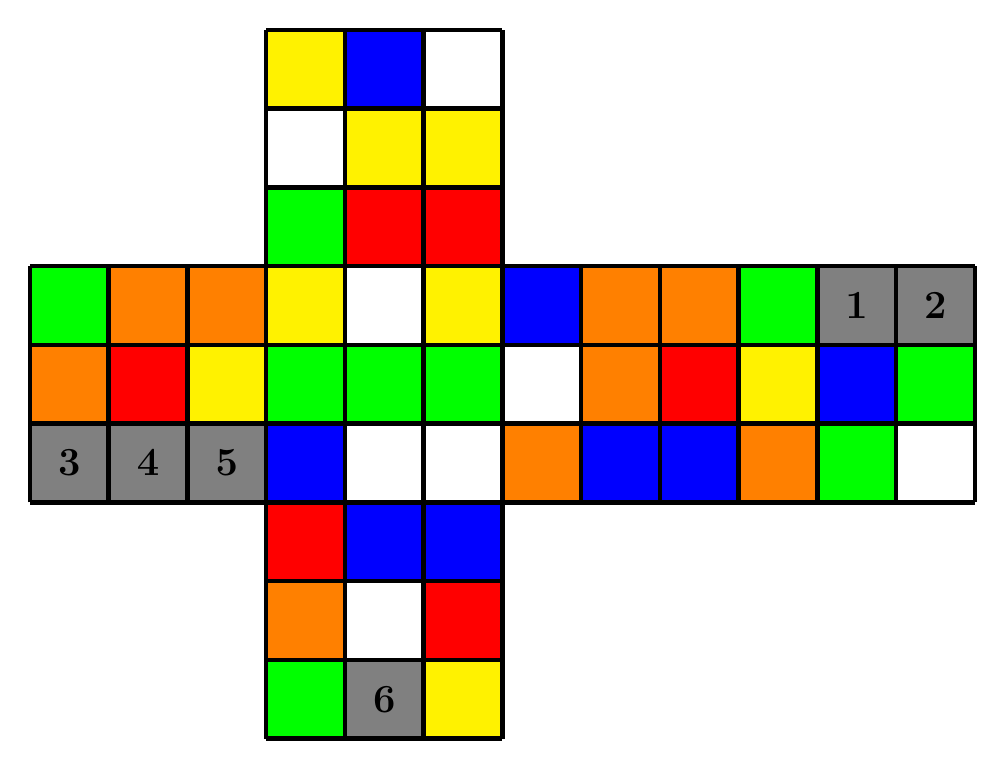
\begin{tikzpicture}[every node/.style={minimum size=1cm-\pgflinewidth, outer sep=0pt}]
\node[fill=yellow] at (0.5,5.5) {};
\node[fill=blue] at (1.5,5.5) {};
\node[fill=white] at (2.5,5.5) {};
\node[fill=white] at (0.5,4.5) {};
\node[fill=yellow] at (1.5,4.5) {};
\node[fill=yellow] at (2.5,4.5) {};
\node[fill=green] at (0.5,3.5) {};
\node[fill=red] at (1.5,3.5) {};
\node[fill=red] at (2.5,3.5) {};

\node[fill=green] at (-2.5,2.5) {};
\node[fill=orange] at (-1.5,2.5) {};
\node[fill=orange] at (-0.5,2.5) {};
\node[fill=yellow] at (0.5,2.5) {};
\node[fill=white] at (1.5,2.5) {};
\node[fill=yellow] at (2.5,2.5) {};
\node[fill=blue] at (3.5,2.5) {};
\node[fill=orange] at (4.5,2.5) {};
\node[fill=orange] at (5.5,2.5) {};
\node[fill=green] at (6.5,2.5) {};
\node[fill=gray] at (7.5,2.5) {\Large \textbf 1};
\node[fill=gray] at (8.5,2.5) {\Large \textbf 2};

\node[fill=orange] at (-2.5,1.5) {};
\node[fill=red] at (-1.5,1.5) {};
\node[fill=yellow] at (-0.5,1.5) {};
\node[fill=green] at (0.5,1.5) {};
\node[fill=green] at (1.5,1.5) {};
\node[fill=green] at (2.5,1.5) {};
\node[fill=white] at (3.5,1.5) {};
\node[fill=orange] at (4.5,1.5) {};
\node[fill=red] at (5.5,1.5) {};
\node[fill=yellow] at (6.5,1.5) {};
\node[fill=blue] at (7.5,1.5) {};
\node[fill=green] at (8.5,1.5) {};

\node[fill=gray] at (-2.5,0.5) {\Large \textbf 3};
\node[fill=gray] at (-1.5,0.5) {\Large \textbf 4};
\node[fill=gray] at (-0.5,0.5) {\Large \textbf 5};
\node[fill=blue] at (0.5,0.5) {};
\node[fill=white] at (1.5,0.5) {};
\node[fill=white] at (2.5,0.5) {};
\node[fill=orange] at (3.5,0.5) {};
\node[fill=blue] at (4.5,0.5) {};
\node[fill=blue] at (5.5,0.5) {};
\node[fill=orange] at (6.5,0.5) {};
\node[fill=green] at (7.5,0.5) {};
\node[fill=white] at (8.5,0.5) {};

\node[fill=red] at (0.5,-0.5) {};
\node[fill=blue] at (1.5,-0.5) {};
\node[fill=blue] at (2.5,-0.5) {};
\node[fill=orange] at (0.5,-1.5) {};
\node[fill=white] at (1.5,-1.5) {};
\node[fill=red] at (2.5,-1.5) {};
\node[fill=green] at (0.5,-2.5) {};
\node[fill=gray] at (1.5,-2.5) {\Large \textbf 6};
\node[fill=yellow] at (2.5,-2.5) {};

\draw[step=1cm,color=black, ultra thick] (-3,0) grid (9,3);
\draw[step=1cm,color=black, ultra thick] (0,-3) grid (3,0);
\draw[step=1cm,color=black, ultra thick] (0,3) grid (3,6);    
\end{tikzpicture}
\vspace{0.1cm}
\\
\noindent\normalsize \newtime  \textbf{Solution 10: B' F2 U' R2 D' B2 U' L2 B2 U' F2 D2 R U2 B' D F R U2 R2 Uw}
\vspace{1cm}



{\noindent\Large \textbf{No. 11\qquad Difficulty:$\bigstar$}}
\vspace{0.2cm}\\
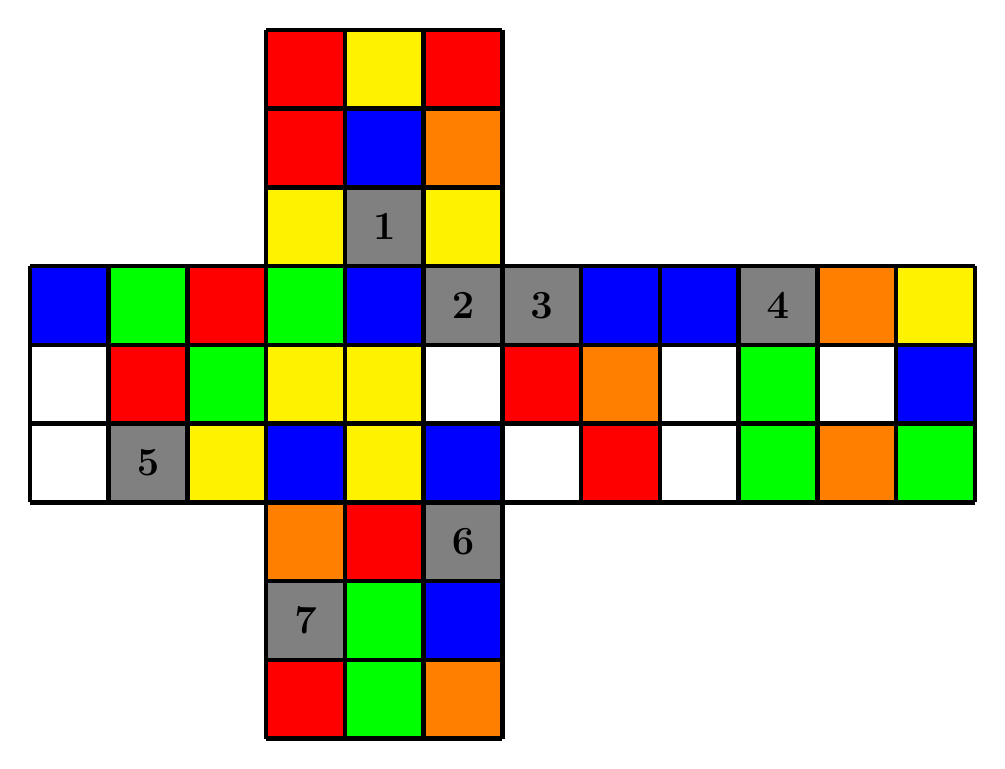
\begin{tikzpicture}[every node/.style={minimum size=1cm-\pgflinewidth, outer sep=0pt}]
\node[fill=red] at (0.5,5.5) {};
\node[fill=yellow] at (1.5,5.5) {};
\node[fill=red] at (2.5,5.5) {};
\node[fill=red] at (0.5,4.5) {};
\node[fill=blue] at (1.5,4.5) {};
\node[fill=orange] at (2.5,4.5) {};
\node[fill=yellow] at (0.5,3.5) {};
\node[fill=gray] at (1.5,3.5) {\Large \textbf 1};
\node[fill=yellow] at (2.5,3.5) {};

\node[fill=blue] at (-2.5,2.5) {};
\node[fill=green] at (-1.5,2.5) {};
\node[fill=red] at (-0.5,2.5) {};
\node[fill=green] at (0.5,2.5) {};
\node[fill=blue] at (1.5,2.5) {};
\node[fill=gray] at (2.5,2.5) {\Large \textbf 2};
\node[fill=gray] at (3.5,2.5) {\Large \textbf 3};
\node[fill=blue] at (4.5,2.5) {};
\node[fill=blue] at (5.5,2.5) {};
\node[fill=gray] at (6.5,2.5) {\Large \textbf 4};
\node[fill=orange] at (7.5,2.5) {};
\node[fill=yellow] at (8.5,2.5) {};

\node[fill=white] at (-2.5,1.5) {};
\node[fill=red] at (-1.5,1.5) {};
\node[fill=green] at (-0.5,1.5) {};
\node[fill=yellow] at (0.5,1.5) {};
\node[fill=yellow] at (1.5,1.5) {};
\node[fill=white] at (2.5,1.5) {};
\node[fill=red] at (3.5,1.5) {};
\node[fill=orange] at (4.5,1.5) {};
\node[fill=white] at (5.5,1.5) {};
\node[fill=green] at (6.5,1.5) {};
\node[fill=white] at (7.5,1.5) {};
\node[fill=blue] at (8.5,1.5) {};

\node[fill=white] at (-2.5,0.5) {};
\node[fill=gray] at (-1.5,0.5) {\Large \textbf 5};
\node[fill=yellow] at (-0.5,0.5) {};
\node[fill=blue] at (0.5,0.5) {};
\node[fill=yellow] at (1.5,0.5) {};
\node[fill=blue] at (2.5,0.5) {};
\node[fill=white] at (3.5,0.5) {};
\node[fill=red] at (4.5,0.5) {};
\node[fill=white] at (5.5,0.5) {};
\node[fill=green] at (6.5,0.5) {};
\node[fill=orange] at (7.5,0.5) {};
\node[fill=green] at (8.5,0.5) {};

\node[fill=orange] at (0.5,-0.5) {};
\node[fill=red] at (1.5,-0.5) {};
\node[fill=gray] at (2.5,-0.5) {\Large \textbf 6};
\node[fill=gray] at (0.5,-1.5) {\Large \textbf 7};
\node[fill=green] at (1.5,-1.5) {};
\node[fill=blue] at (2.5,-1.5) {};
\node[fill=red] at (0.5,-2.5) {};
\node[fill=green] at (1.5,-2.5) {};
\node[fill=orange] at (2.5,-2.5) {};

\draw[step=1cm,color=black, ultra thick] (-3,0) grid (9,3);
\draw[step=1cm,color=black, ultra thick] (0,-3) grid (3,0);
\draw[step=1cm,color=black, ultra thick] (0,3) grid (3,6);    
\end{tikzpicture}
\vspace{0.1cm}
\\
\noindent\normalsize \newtime  \textbf{Solution 11: D2 L2 F2 L2 R2 D2 F' R2 U2 B' L2 F' U' B' D B R B D' L Fw Uw}
\vspace{1cm}



{\noindent\Large \textbf{No. 12\qquad Difficulty:$\bigstar$}}
\vspace{0.2cm}\\
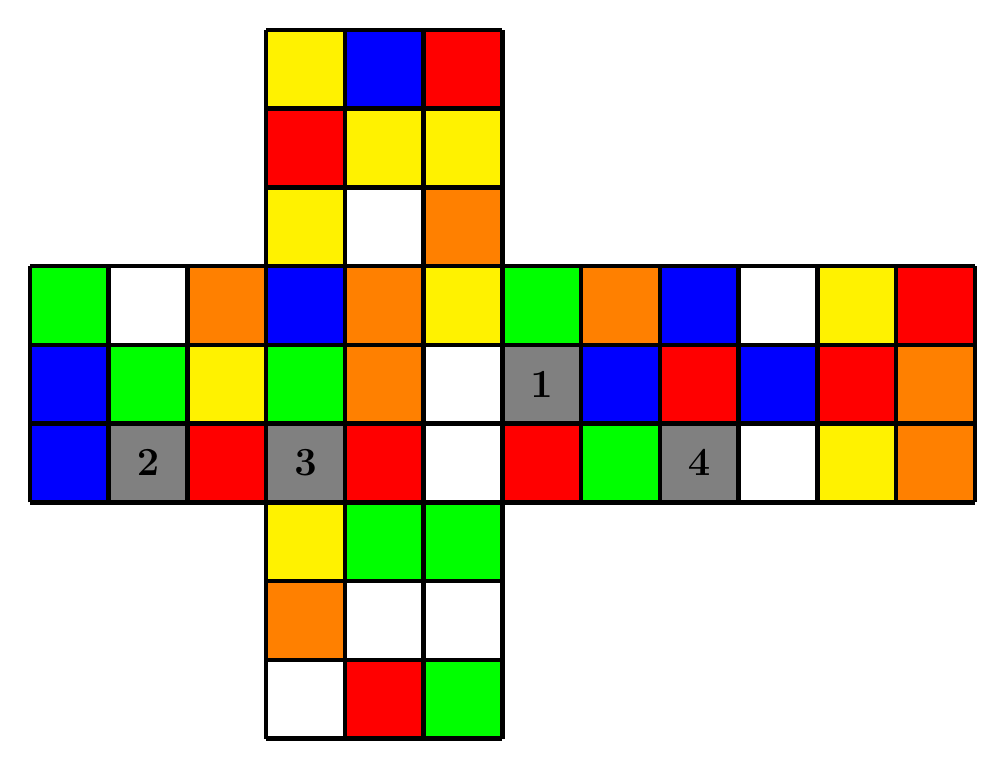
\begin{tikzpicture}[every node/.style={minimum size=1cm-\pgflinewidth, outer sep=0pt}]
\node[fill=yellow] at (0.5,5.5) {};
\node[fill=blue] at (1.5,5.5) {};
\node[fill=red] at (2.5,5.5) {};
\node[fill=red] at (0.5,4.5) {};
\node[fill=yellow] at (1.5,4.5) {};
\node[fill=yellow] at (2.5,4.5) {};
\node[fill=yellow] at (0.5,3.5) {};
\node[fill=white] at (1.5,3.5) {};
\node[fill=orange] at (2.5,3.5) {};

\node[fill=green] at (-2.5,2.5) {};
\node[fill=white] at (-1.5,2.5) {};
\node[fill=orange] at (-0.5,2.5) {};
\node[fill=blue] at (0.5,2.5) {};
\node[fill=orange] at (1.5,2.5) {};
\node[fill=yellow] at (2.5,2.5) {};
\node[fill=green] at (3.5,2.5) {};
\node[fill=orange] at (4.5,2.5) {};
\node[fill=blue] at (5.5,2.5) {};
\node[fill=white] at (6.5,2.5) {};
\node[fill=yellow] at (7.5,2.5) {};
\node[fill=red] at (8.5,2.5) {};

\node[fill=blue] at (-2.5,1.5) {};
\node[fill=green] at (-1.5,1.5) {};
\node[fill=yellow] at (-0.5,1.5) {};
\node[fill=green] at (0.5,1.5) {};
\node[fill=orange] at (1.5,1.5) {};
\node[fill=white] at (2.5,1.5) {};
\node[fill=gray] at (3.5,1.5) {\Large \textbf 1};
\node[fill=blue] at (4.5,1.5) {};
\node[fill=red] at (5.5,1.5) {};
\node[fill=blue] at (6.5,1.5) {};
\node[fill=red] at (7.5,1.5) {};
\node[fill=orange] at (8.5,1.5) {};

\node[fill=blue] at (-2.5,0.5) {};
\node[fill=gray] at (-1.5,0.5) {\Large \textbf 2};
\node[fill=red] at (-0.5,0.5) {};
\node[fill=gray] at (0.5,0.5) {\Large \textbf 3};
\node[fill=red] at (1.5,0.5) {};
\node[fill=white] at (2.5,0.5) {};
\node[fill=red] at (3.5,0.5) {};
\node[fill=green] at (4.5,0.5) {};
\node[fill=gray] at (5.5,0.5) {\Large \textbf 4};
\node[fill=white] at (6.5,0.5) {};
\node[fill=yellow] at (7.5,0.5) {};
\node[fill=orange] at (8.5,0.5) {};

\node[fill=yellow] at (0.5,-0.5) {};
\node[fill=green] at (1.5,-0.5) {};
\node[fill=green] at (2.5,-0.5) {};
\node[fill=orange] at (0.5,-1.5) {};
\node[fill=white] at (1.5,-1.5) {};
\node[fill=white] at (2.5,-1.5) {};
\node[fill=white] at (0.5,-2.5) {};
\node[fill=red] at (1.5,-2.5) {};
\node[fill=green] at (2.5,-2.5) {};

\draw[step=1cm,color=black, ultra thick] (-3,0) grid (9,3);
\draw[step=1cm,color=black, ultra thick] (0,-3) grid (3,0);
\draw[step=1cm,color=black, ultra thick] (0,3) grid (3,6);    
\end{tikzpicture}
\vspace{0.1cm}
\\
\noindent\normalsize \newtime  \textbf{Solution 12: F' L R2 U B2 U2 B2 L2 R2 U' L2 D2 R2 D' R F U2 F U2 R2 D2 Uw2}
\vspace{1cm}



{\noindent\Large \textbf{No. 13\qquad Difficulty:$\bigstar$}}
\vspace{0.2cm}\\
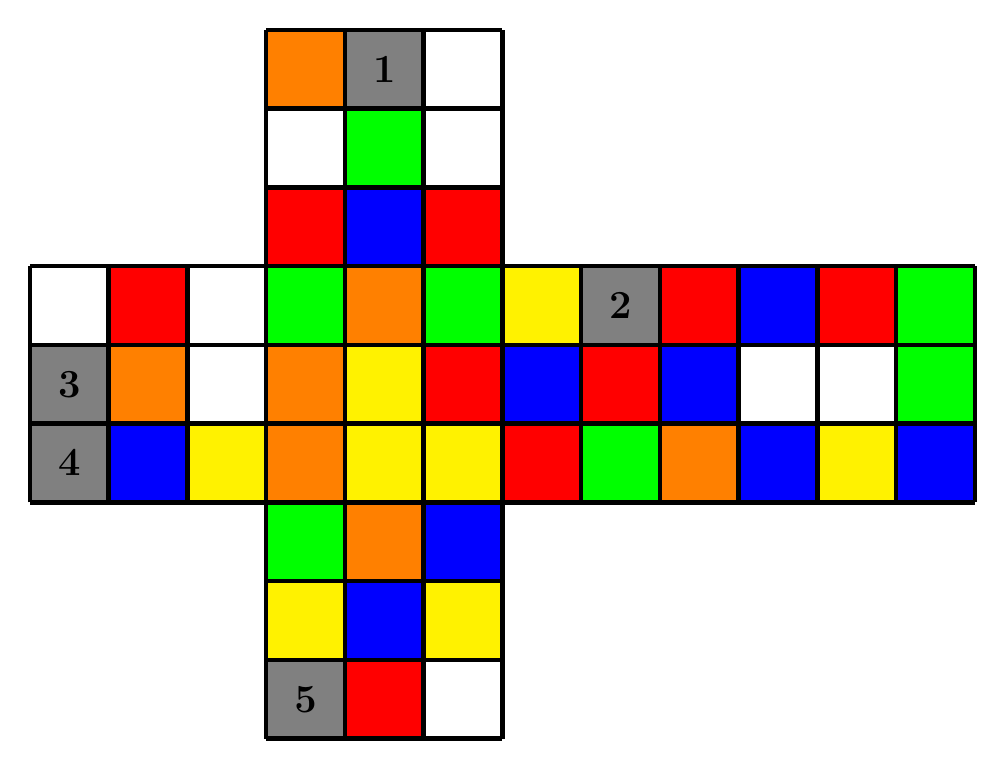
\begin{tikzpicture}[every node/.style={minimum size=1cm-\pgflinewidth, outer sep=0pt}]
\node[fill=orange] at (0.5,5.5) {};
\node[fill=gray] at (1.5,5.5) {\Large \textbf 1};
\node[fill=white] at (2.5,5.5) {};
\node[fill=white] at (0.5,4.5) {};
\node[fill=green] at (1.5,4.5) {};
\node[fill=white] at (2.5,4.5) {};
\node[fill=red] at (0.5,3.5) {};
\node[fill=blue] at (1.5,3.5) {};
\node[fill=red] at (2.5,3.5) {};

\node[fill=white] at (-2.5,2.5) {};
\node[fill=red] at (-1.5,2.5) {};
\node[fill=white] at (-0.5,2.5) {};
\node[fill=green] at (0.5,2.5) {};
\node[fill=orange] at (1.5,2.5) {};
\node[fill=green] at (2.5,2.5) {};
\node[fill=yellow] at (3.5,2.5) {};
\node[fill=gray] at (4.5,2.5) {\Large \textbf 2};
\node[fill=red] at (5.5,2.5) {};
\node[fill=blue] at (6.5,2.5) {};
\node[fill=red] at (7.5,2.5) {};
\node[fill=green] at (8.5,2.5) {};

\node[fill=gray] at (-2.5,1.5) {\Large \textbf 3};
\node[fill=orange] at (-1.5,1.5) {};
\node[fill=white] at (-0.5,1.5) {};
\node[fill=orange] at (0.5,1.5) {};
\node[fill=yellow] at (1.5,1.5) {};
\node[fill=red] at (2.5,1.5) {};
\node[fill=blue] at (3.5,1.5) {};
\node[fill=red] at (4.5,1.5) {};
\node[fill=blue] at (5.5,1.5) {};
\node[fill=white] at (6.5,1.5) {};
\node[fill=white] at (7.5,1.5) {};
\node[fill=green] at (8.5,1.5) {};

\node[fill=gray] at (-2.5,0.5) {\Large \textbf 4};
\node[fill=blue] at (-1.5,0.5) {};
\node[fill=yellow] at (-0.5,0.5) {};
\node[fill=orange] at (0.5,0.5) {};
\node[fill=yellow] at (1.5,0.5) {};
\node[fill=yellow] at (2.5,0.5) {};
\node[fill=red] at (3.5,0.5) {};
\node[fill=green] at (4.5,0.5) {};
\node[fill=orange] at (5.5,0.5) {};
\node[fill=blue] at (6.5,0.5) {};
\node[fill=yellow] at (7.5,0.5) {};
\node[fill=blue] at (8.5,0.5) {};

\node[fill=green] at (0.5,-0.5) {};
\node[fill=orange] at (1.5,-0.5) {};
\node[fill=blue] at (2.5,-0.5) {};
\node[fill=yellow] at (0.5,-1.5) {};
\node[fill=blue] at (1.5,-1.5) {};
\node[fill=yellow] at (2.5,-1.5) {};
\node[fill=gray] at (0.5,-2.5) {\Large \textbf 5};
\node[fill=red] at (1.5,-2.5) {};
\node[fill=white] at (2.5,-2.5) {};

\draw[step=1cm,color=black, ultra thick] (-3,0) grid (9,3);
\draw[step=1cm,color=black, ultra thick] (0,-3) grid (3,0);
\draw[step=1cm,color=black, ultra thick] (0,3) grid (3,6);    
\end{tikzpicture}
\vspace{0.1cm}
\\
\noindent\normalsize \newtime  \textbf{Solution 13: F U B' U2 R F B R2 D F2 R2 U2 R' U2 L' D2 L2 D2 F2 R' U2 Fw' Uw'}
\vspace{1cm}



{\noindent\Large \textbf{No. 14\qquad Difficulty:$\bigstar$}}
\vspace{0.2cm}\\
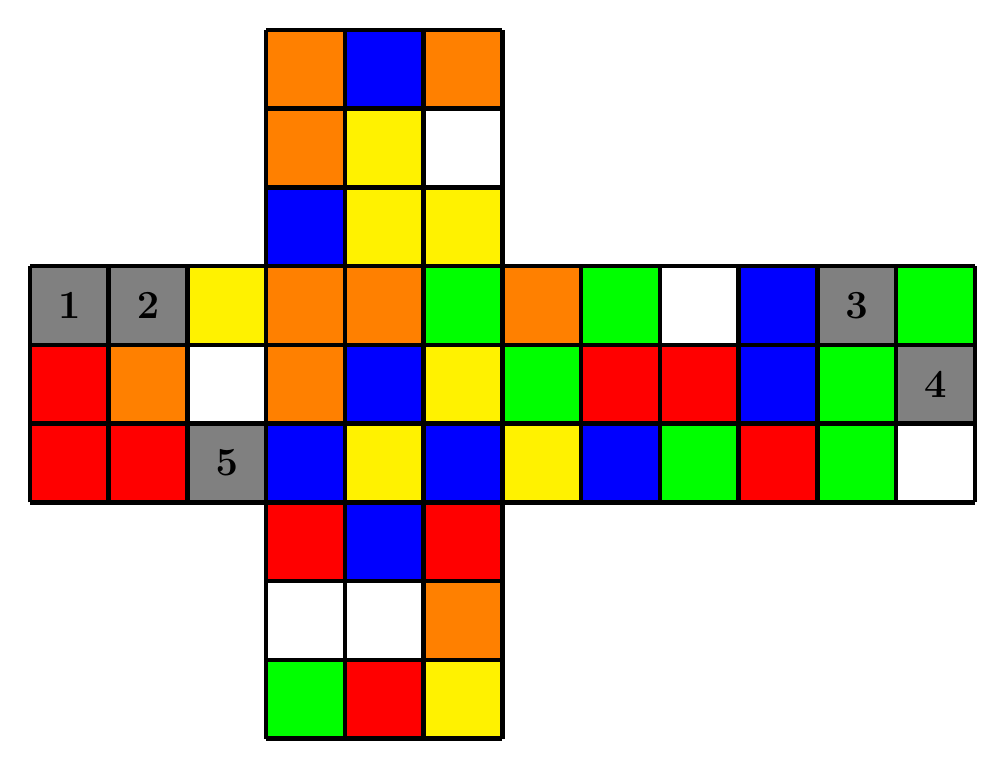
\begin{tikzpicture}[every node/.style={minimum size=1cm-\pgflinewidth, outer sep=0pt}]
\node[fill=orange] at (0.5,5.5) {};
\node[fill=blue] at (1.5,5.5) {};
\node[fill=orange] at (2.5,5.5) {};
\node[fill=orange] at (0.5,4.5) {};
\node[fill=yellow] at (1.5,4.5) {};
\node[fill=white] at (2.5,4.5) {};
\node[fill=blue] at (0.5,3.5) {};
\node[fill=yellow] at (1.5,3.5) {};
\node[fill=yellow] at (2.5,3.5) {};

\node[fill=gray] at (-2.5,2.5) {\Large \textbf 1};
\node[fill=gray] at (-1.5,2.5) {\Large \textbf 2};
\node[fill=yellow] at (-0.5,2.5) {};
\node[fill=orange] at (0.5,2.5) {};
\node[fill=orange] at (1.5,2.5) {};
\node[fill=green] at (2.5,2.5) {};
\node[fill=orange] at (3.5,2.5) {};
\node[fill=green] at (4.5,2.5) {};
\node[fill=white] at (5.5,2.5) {};
\node[fill=blue] at (6.5,2.5) {};
\node[fill=gray] at (7.5,2.5) {\Large \textbf 3};
\node[fill=green] at (8.5,2.5) {};

\node[fill=red] at (-2.5,1.5) {};
\node[fill=orange] at (-1.5,1.5) {};
\node[fill=white] at (-0.5,1.5) {};
\node[fill=orange] at (0.5,1.5) {};
\node[fill=blue] at (1.5,1.5) {};
\node[fill=yellow] at (2.5,1.5) {};
\node[fill=green] at (3.5,1.5) {};
\node[fill=red] at (4.5,1.5) {};
\node[fill=red] at (5.5,1.5) {};
\node[fill=blue] at (6.5,1.5) {};
\node[fill=green] at (7.5,1.5) {};
\node[fill=gray] at (8.5,1.5) {\Large \textbf 4};

\node[fill=red] at (-2.5,0.5) {};
\node[fill=red] at (-1.5,0.5) {};
\node[fill=gray] at (-0.5,0.5) {\Large \textbf 5};
\node[fill=blue] at (0.5,0.5) {};
\node[fill=yellow] at (1.5,0.5) {};
\node[fill=blue] at (2.5,0.5) {};
\node[fill=yellow] at (3.5,0.5) {};
\node[fill=blue] at (4.5,0.5) {};
\node[fill=green] at (5.5,0.5) {};
\node[fill=red] at (6.5,0.5) {};
\node[fill=green] at (7.5,0.5) {};
\node[fill=white] at (8.5,0.5) {};

\node[fill=red] at (0.5,-0.5) {};
\node[fill=blue] at (1.5,-0.5) {};
\node[fill=red] at (2.5,-0.5) {};
\node[fill=white] at (0.5,-1.5) {};
\node[fill=white] at (1.5,-1.5) {};
\node[fill=orange] at (2.5,-1.5) {};
\node[fill=green] at (0.5,-2.5) {};
\node[fill=red] at (1.5,-2.5) {};
\node[fill=yellow] at (2.5,-2.5) {};

\draw[step=1cm,color=black, ultra thick] (-3,0) grid (9,3);
\draw[step=1cm,color=black, ultra thick] (0,-3) grid (3,0);
\draw[step=1cm,color=black, ultra thick] (0,3) grid (3,6);    
\end{tikzpicture}
\vspace{0.1cm}
\\
\noindent\normalsize \newtime  \textbf{Solution 14: L' D' R2 B' L2 D2 U2 B R2 B2 R2 F' U2 B2 R' F2 D L2 U' F R2 Uw'}
\vspace{1cm}



{\noindent\Large \textbf{No. 15\qquad Difficulty:$\bigstar$}}
\vspace{0.2cm}\\
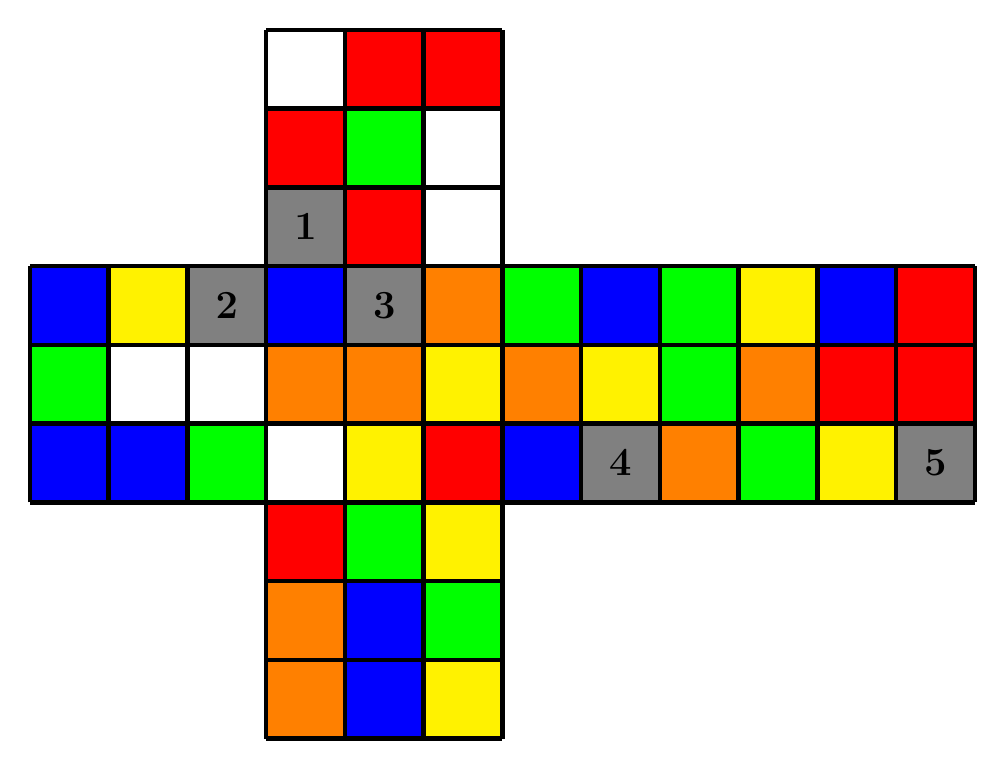
\begin{tikzpicture}[every node/.style={minimum size=1cm-\pgflinewidth, outer sep=0pt}]
\node[fill=white] at (0.5,5.5) {};
\node[fill=red] at (1.5,5.5) {};
\node[fill=red] at (2.5,5.5) {};
\node[fill=red] at (0.5,4.5) {};
\node[fill=green] at (1.5,4.5) {};
\node[fill=white] at (2.5,4.5) {};
\node[fill=gray] at (0.5,3.5) {\Large \textbf 1};
\node[fill=red] at (1.5,3.5) {};
\node[fill=white] at (2.5,3.5) {};

\node[fill=blue] at (-2.5,2.5) {};
\node[fill=yellow] at (-1.5,2.5) {};
\node[fill=gray] at (-0.5,2.5) {\Large \textbf 2};
\node[fill=blue] at (0.5,2.5) {};
\node[fill=gray] at (1.5,2.5) {\Large \textbf 3};
\node[fill=orange] at (2.5,2.5) {};
\node[fill=green] at (3.5,2.5) {};
\node[fill=blue] at (4.5,2.5) {};
\node[fill=green] at (5.5,2.5) {};
\node[fill=yellow] at (6.5,2.5) {};
\node[fill=blue] at (7.5,2.5) {};
\node[fill=red] at (8.5,2.5) {};

\node[fill=green] at (-2.5,1.5) {};
\node[fill=white] at (-1.5,1.5) {};
\node[fill=white] at (-0.5,1.5) {};
\node[fill=orange] at (0.5,1.5) {};
\node[fill=orange] at (1.5,1.5) {};
\node[fill=yellow] at (2.5,1.5) {};
\node[fill=orange] at (3.5,1.5) {};
\node[fill=yellow] at (4.5,1.5) {};
\node[fill=green] at (5.5,1.5) {};
\node[fill=orange] at (6.5,1.5) {};
\node[fill=red] at (7.5,1.5) {};
\node[fill=red] at (8.5,1.5) {};

\node[fill=blue] at (-2.5,0.5) {};
\node[fill=blue] at (-1.5,0.5) {};
\node[fill=green] at (-0.5,0.5) {};
\node[fill=white] at (0.5,0.5) {};
\node[fill=yellow] at (1.5,0.5) {};
\node[fill=red] at (2.5,0.5) {};
\node[fill=blue] at (3.5,0.5) {};
\node[fill=gray] at (4.5,0.5) {\Large \textbf 4};
\node[fill=orange] at (5.5,0.5) {};
\node[fill=green] at (6.5,0.5) {};
\node[fill=yellow] at (7.5,0.5) {};
\node[fill=gray] at (8.5,0.5) {\Large \textbf 5};

\node[fill=red] at (0.5,-0.5) {};
\node[fill=green] at (1.5,-0.5) {};
\node[fill=yellow] at (2.5,-0.5) {};
\node[fill=orange] at (0.5,-1.5) {};
\node[fill=blue] at (1.5,-1.5) {};
\node[fill=green] at (2.5,-1.5) {};
\node[fill=orange] at (0.5,-2.5) {};
\node[fill=blue] at (1.5,-2.5) {};
\node[fill=yellow] at (2.5,-2.5) {};

\draw[step=1cm,color=black, ultra thick] (-3,0) grid (9,3);
\draw[step=1cm,color=black, ultra thick] (0,-3) grid (3,0);
\draw[step=1cm,color=black, ultra thick] (0,3) grid (3,6);    
\end{tikzpicture}
\vspace{0.1cm}
\\
\noindent\normalsize \newtime  \textbf{Solution 15: B D' R2 D2 B L2 B' L2 F R2 B' F2 U2 L' R D F D2 B' L F' Fw' Uw2}
\vspace{1cm}



{\noindent\Large \textbf{No. 16\qquad Difficulty:$\bigstar$}}
\vspace{0.2cm}\\
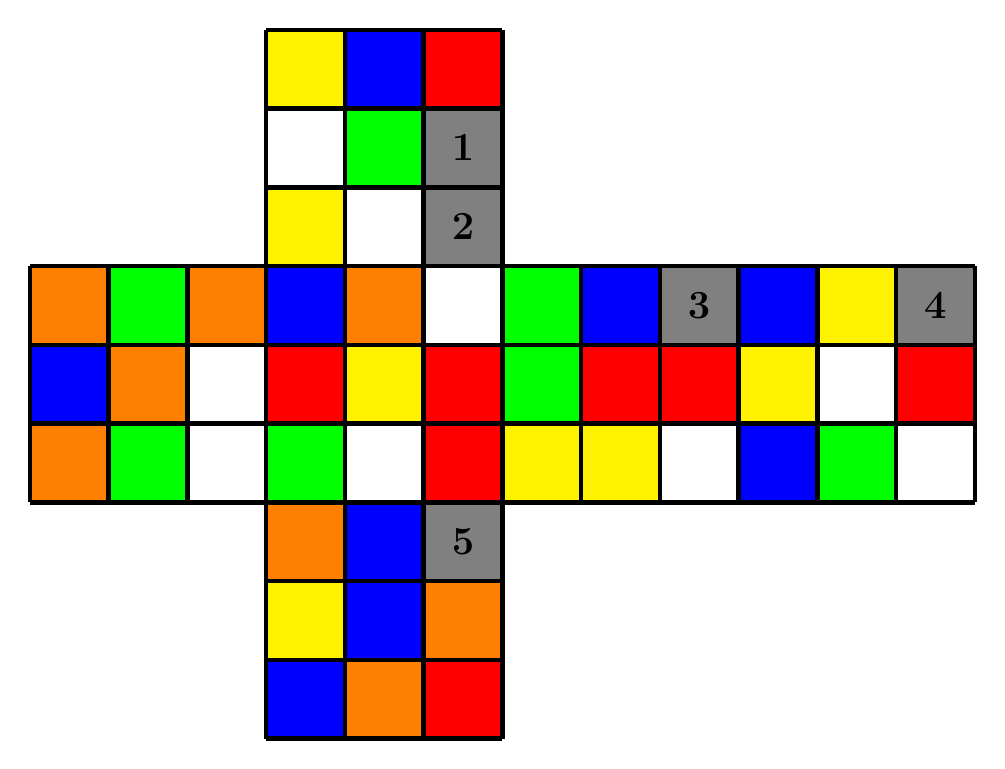
\begin{tikzpicture}[every node/.style={minimum size=1cm-\pgflinewidth, outer sep=0pt}]
\node[fill=yellow] at (0.5,5.5) {};
\node[fill=blue] at (1.5,5.5) {};
\node[fill=red] at (2.5,5.5) {};
\node[fill=white] at (0.5,4.5) {};
\node[fill=green] at (1.5,4.5) {};
\node[fill=gray] at (2.5,4.5) {\Large \textbf 1};
\node[fill=yellow] at (0.5,3.5) {};
\node[fill=white] at (1.5,3.5) {};
\node[fill=gray] at (2.5,3.5) {\Large \textbf 2};

\node[fill=orange] at (-2.5,2.5) {};
\node[fill=green] at (-1.5,2.5) {};
\node[fill=orange] at (-0.5,2.5) {};
\node[fill=blue] at (0.5,2.5) {};
\node[fill=orange] at (1.5,2.5) {};
\node[fill=white] at (2.5,2.5) {};
\node[fill=green] at (3.5,2.5) {};
\node[fill=blue] at (4.5,2.5) {};
\node[fill=gray] at (5.5,2.5) {\Large \textbf 3};
\node[fill=blue] at (6.5,2.5) {};
\node[fill=yellow] at (7.5,2.5) {};
\node[fill=gray] at (8.5,2.5) {\Large \textbf 4};

\node[fill=blue] at (-2.5,1.5) {};
\node[fill=orange] at (-1.5,1.5) {};
\node[fill=white] at (-0.5,1.5) {};
\node[fill=red] at (0.5,1.5) {};
\node[fill=yellow] at (1.5,1.5) {};
\node[fill=red] at (2.5,1.5) {};
\node[fill=green] at (3.5,1.5) {};
\node[fill=red] at (4.5,1.5) {};
\node[fill=red] at (5.5,1.5) {};
\node[fill=yellow] at (6.5,1.5) {};
\node[fill=white] at (7.5,1.5) {};
\node[fill=red] at (8.5,1.5) {};

\node[fill=orange] at (-2.5,0.5) {};
\node[fill=green] at (-1.5,0.5) {};
\node[fill=white] at (-0.5,0.5) {};
\node[fill=green] at (0.5,0.5) {};
\node[fill=white] at (1.5,0.5) {};
\node[fill=red] at (2.5,0.5) {};
\node[fill=yellow] at (3.5,0.5) {};
\node[fill=yellow] at (4.5,0.5) {};
\node[fill=white] at (5.5,0.5) {};
\node[fill=blue] at (6.5,0.5) {};
\node[fill=green] at (7.5,0.5) {};
\node[fill=white] at (8.5,0.5) {};

\node[fill=orange] at (0.5,-0.5) {};
\node[fill=blue] at (1.5,-0.5) {};
\node[fill=gray] at (2.5,-0.5) {\Large \textbf 5};
\node[fill=yellow] at (0.5,-1.5) {};
\node[fill=blue] at (1.5,-1.5) {};
\node[fill=orange] at (2.5,-1.5) {};
\node[fill=blue] at (0.5,-2.5) {};
\node[fill=orange] at (1.5,-2.5) {};
\node[fill=red] at (2.5,-2.5) {};

\draw[step=1cm,color=black, ultra thick] (-3,0) grid (9,3);
\draw[step=1cm,color=black, ultra thick] (0,-3) grid (3,0);
\draw[step=1cm,color=black, ultra thick] (0,3) grid (3,6);    
\end{tikzpicture}
\vspace{0.1cm}
\\
\noindent\normalsize \newtime  \textbf{Solution 16: R' F2 L' D2 L' U2 R' F2 R' F2 D2 U' B D2 L' F2 R2 D2 U R Fw' Uw'}
\vspace{1cm}



{\noindent\Large \textbf{No. 17\qquad Difficulty:$\bigstar$}}
\vspace{0.2cm}\\
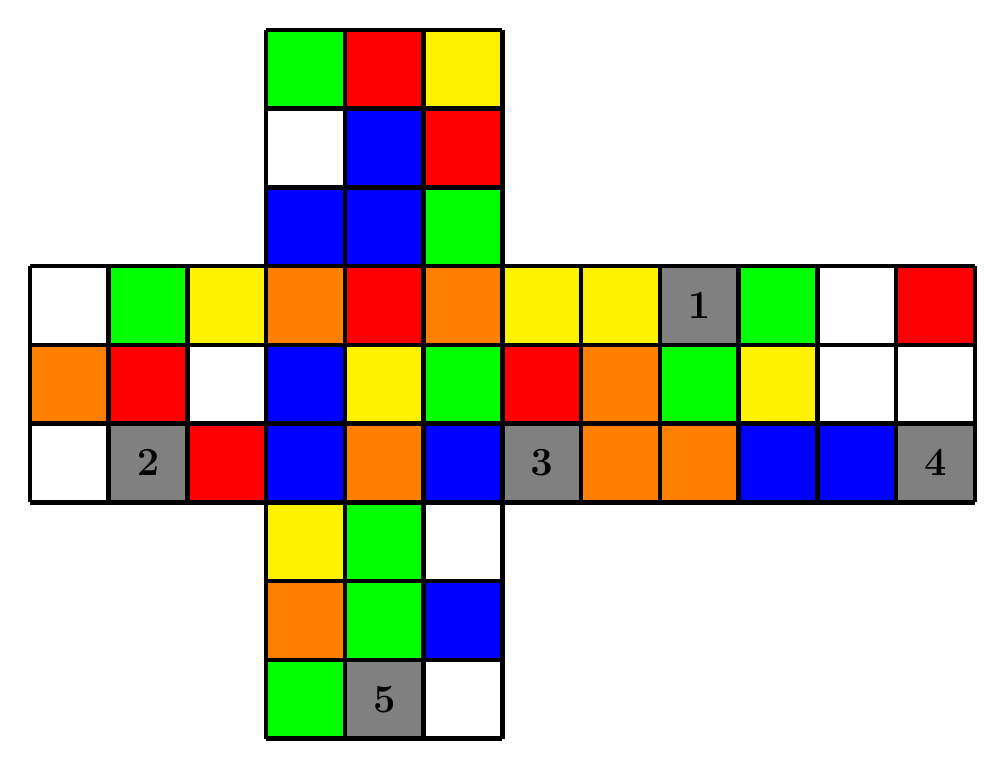
\begin{tikzpicture}[every node/.style={minimum size=1cm-\pgflinewidth, outer sep=0pt}]
\node[fill=green] at (0.5,5.5) {};
\node[fill=red] at (1.5,5.5) {};
\node[fill=yellow] at (2.5,5.5) {};
\node[fill=white] at (0.5,4.5) {};
\node[fill=blue] at (1.5,4.5) {};
\node[fill=red] at (2.5,4.5) {};
\node[fill=blue] at (0.5,3.5) {};
\node[fill=blue] at (1.5,3.5) {};
\node[fill=green] at (2.5,3.5) {};

\node[fill=white] at (-2.5,2.5) {};
\node[fill=green] at (-1.5,2.5) {};
\node[fill=yellow] at (-0.5,2.5) {};
\node[fill=orange] at (0.5,2.5) {};
\node[fill=red] at (1.5,2.5) {};
\node[fill=orange] at (2.5,2.5) {};
\node[fill=yellow] at (3.5,2.5) {};
\node[fill=yellow] at (4.5,2.5) {};
\node[fill=gray] at (5.5,2.5) {\Large \textbf 1};
\node[fill=green] at (6.5,2.5) {};
\node[fill=white] at (7.5,2.5) {};
\node[fill=red] at (8.5,2.5) {};

\node[fill=orange] at (-2.5,1.5) {};
\node[fill=red] at (-1.5,1.5) {};
\node[fill=white] at (-0.5,1.5) {};
\node[fill=blue] at (0.5,1.5) {};
\node[fill=yellow] at (1.5,1.5) {};
\node[fill=green] at (2.5,1.5) {};
\node[fill=red] at (3.5,1.5) {};
\node[fill=orange] at (4.5,1.5) {};
\node[fill=green] at (5.5,1.5) {};
\node[fill=yellow] at (6.5,1.5) {};
\node[fill=white] at (7.5,1.5) {};
\node[fill=white] at (8.5,1.5) {};

\node[fill=white] at (-2.5,0.5) {};
\node[fill=gray] at (-1.5,0.5) {\Large \textbf 2};
\node[fill=red] at (-0.5,0.5) {};
\node[fill=blue] at (0.5,0.5) {};
\node[fill=orange] at (1.5,0.5) {};
\node[fill=blue] at (2.5,0.5) {};
\node[fill=gray] at (3.5,0.5) {\Large \textbf 3};
\node[fill=orange] at (4.5,0.5) {};
\node[fill=orange] at (5.5,0.5) {};
\node[fill=blue] at (6.5,0.5) {};
\node[fill=blue] at (7.5,0.5) {};
\node[fill=gray] at (8.5,0.5) {\Large \textbf 4};

\node[fill=yellow] at (0.5,-0.5) {};
\node[fill=green] at (1.5,-0.5) {};
\node[fill=white] at (2.5,-0.5) {};
\node[fill=orange] at (0.5,-1.5) {};
\node[fill=green] at (1.5,-1.5) {};
\node[fill=blue] at (2.5,-1.5) {};
\node[fill=green] at (0.5,-2.5) {};
\node[fill=gray] at (1.5,-2.5) {\Large \textbf 5};
\node[fill=white] at (2.5,-2.5) {};

\draw[step=1cm,color=black, ultra thick] (-3,0) grid (9,3);
\draw[step=1cm,color=black, ultra thick] (0,-3) grid (3,0);
\draw[step=1cm,color=black, ultra thick] (0,3) grid (3,6);    
\end{tikzpicture}
\vspace{0.1cm}
\\
\noindent\normalsize \newtime  \textbf{Solution 17: R' F' U2 F2 R' U2 L U2 B2 L2 R' D2 R' F2 U F R2 D2 B D L' Fw Uw}
\vspace{1cm}



{\noindent\Large \textbf{No. 18\qquad Difficulty:$\bigstar$}}
\vspace{0.2cm}\\
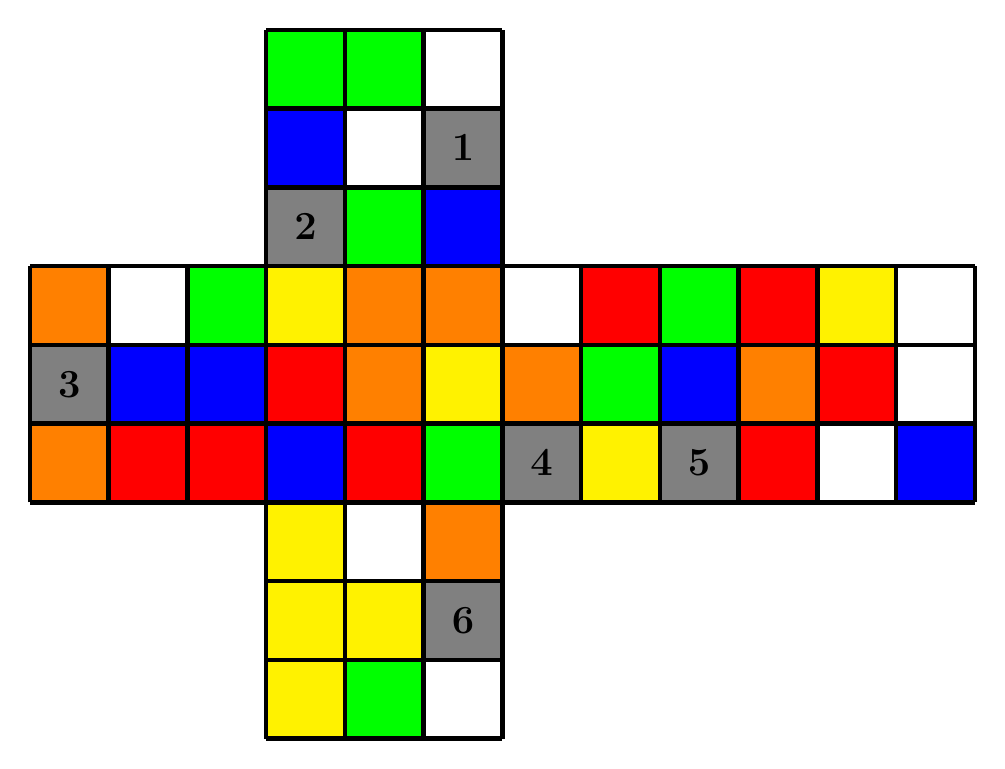
\begin{tikzpicture}[every node/.style={minimum size=1cm-\pgflinewidth, outer sep=0pt}]
\node[fill=green] at (0.5,5.5) {};
\node[fill=green] at (1.5,5.5) {};
\node[fill=white] at (2.5,5.5) {};
\node[fill=blue] at (0.5,4.5) {};
\node[fill=white] at (1.5,4.5) {};
\node[fill=gray] at (2.5,4.5) {\Large \textbf 1};
\node[fill=gray] at (0.5,3.5) {\Large \textbf 2};
\node[fill=green] at (1.5,3.5) {};
\node[fill=blue] at (2.5,3.5) {};

\node[fill=orange] at (-2.5,2.5) {};
\node[fill=white] at (-1.5,2.5) {};
\node[fill=green] at (-0.5,2.5) {};
\node[fill=yellow] at (0.5,2.5) {};
\node[fill=orange] at (1.5,2.5) {};
\node[fill=orange] at (2.5,2.5) {};
\node[fill=white] at (3.5,2.5) {};
\node[fill=red] at (4.5,2.5) {};
\node[fill=green] at (5.5,2.5) {};
\node[fill=red] at (6.5,2.5) {};
\node[fill=yellow] at (7.5,2.5) {};
\node[fill=white] at (8.5,2.5) {};

\node[fill=gray] at (-2.5,1.5) {\Large \textbf 3};
\node[fill=blue] at (-1.5,1.5) {};
\node[fill=blue] at (-0.5,1.5) {};
\node[fill=red] at (0.5,1.5) {};
\node[fill=orange] at (1.5,1.5) {};
\node[fill=yellow] at (2.5,1.5) {};
\node[fill=orange] at (3.5,1.5) {};
\node[fill=green] at (4.5,1.5) {};
\node[fill=blue] at (5.5,1.5) {};
\node[fill=orange] at (6.5,1.5) {};
\node[fill=red] at (7.5,1.5) {};
\node[fill=white] at (8.5,1.5) {};

\node[fill=orange] at (-2.5,0.5) {};
\node[fill=red] at (-1.5,0.5) {};
\node[fill=red] at (-0.5,0.5) {};
\node[fill=blue] at (0.5,0.5) {};
\node[fill=red] at (1.5,0.5) {};
\node[fill=green] at (2.5,0.5) {};
\node[fill=gray] at (3.5,0.5) {\Large \textbf 4};
\node[fill=yellow] at (4.5,0.5) {};
\node[fill=gray] at (5.5,0.5) {\Large \textbf 5};
\node[fill=red] at (6.5,0.5) {};
\node[fill=white] at (7.5,0.5) {};
\node[fill=blue] at (8.5,0.5) {};

\node[fill=yellow] at (0.5,-0.5) {};
\node[fill=white] at (1.5,-0.5) {};
\node[fill=orange] at (2.5,-0.5) {};
\node[fill=yellow] at (0.5,-1.5) {};
\node[fill=yellow] at (1.5,-1.5) {};
\node[fill=gray] at (2.5,-1.5) {\Large \textbf 6};
\node[fill=yellow] at (0.5,-2.5) {};
\node[fill=green] at (1.5,-2.5) {};
\node[fill=white] at (2.5,-2.5) {};

\draw[step=1cm,color=black, ultra thick] (-3,0) grid (9,3);
\draw[step=1cm,color=black, ultra thick] (0,-3) grid (3,0);
\draw[step=1cm,color=black, ultra thick] (0,3) grid (3,6);    
\end{tikzpicture}
\vspace{0.1cm}
\\
\noindent\normalsize \newtime  \textbf{Solution 18: L D B U2 L D F' R' U B2 U2 B' L2 B' L2 U2 L2 F2 R2 D2 F2 Rw2}
\vspace{1cm}



{\noindent\Large \textbf{No. 19\qquad Difficulty:$\bigstar$}}
\vspace{0.2cm}\\
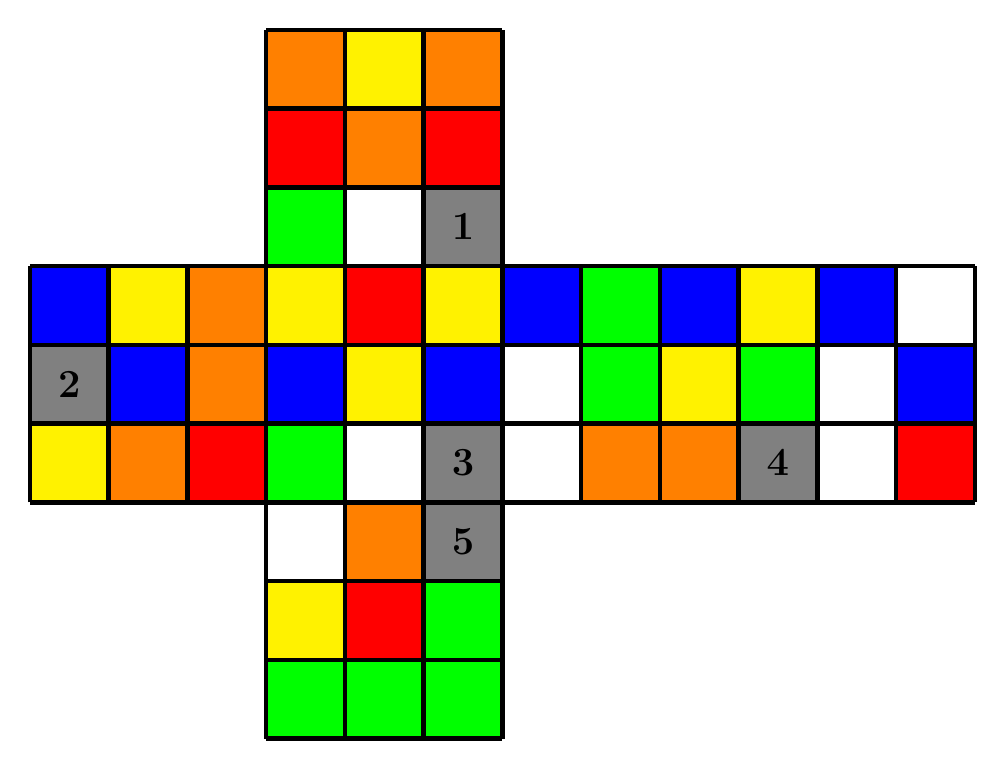
\begin{tikzpicture}[every node/.style={minimum size=1cm-\pgflinewidth, outer sep=0pt}]
\node[fill=orange] at (0.5,5.5) {};
\node[fill=yellow] at (1.5,5.5) {};
\node[fill=orange] at (2.5,5.5) {};
\node[fill=red] at (0.5,4.5) {};
\node[fill=orange] at (1.5,4.5) {};
\node[fill=red] at (2.5,4.5) {};
\node[fill=green] at (0.5,3.5) {};
\node[fill=white] at (1.5,3.5) {};
\node[fill=gray] at (2.5,3.5) {\Large \textbf 1};

\node[fill=blue] at (-2.5,2.5) {};
\node[fill=yellow] at (-1.5,2.5) {};
\node[fill=orange] at (-0.5,2.5) {};
\node[fill=yellow] at (0.5,2.5) {};
\node[fill=red] at (1.5,2.5) {};
\node[fill=yellow] at (2.5,2.5) {};
\node[fill=blue] at (3.5,2.5) {};
\node[fill=green] at (4.5,2.5) {};
\node[fill=blue] at (5.5,2.5) {};
\node[fill=yellow] at (6.5,2.5) {};
\node[fill=blue] at (7.5,2.5) {};
\node[fill=white] at (8.5,2.5) {};

\node[fill=gray] at (-2.5,1.5) {\Large \textbf 2};
\node[fill=blue] at (-1.5,1.5) {};
\node[fill=orange] at (-0.5,1.5) {};
\node[fill=blue] at (0.5,1.5) {};
\node[fill=yellow] at (1.5,1.5) {};
\node[fill=blue] at (2.5,1.5) {};
\node[fill=white] at (3.5,1.5) {};
\node[fill=green] at (4.5,1.5) {};
\node[fill=yellow] at (5.5,1.5) {};
\node[fill=green] at (6.5,1.5) {};
\node[fill=white] at (7.5,1.5) {};
\node[fill=blue] at (8.5,1.5) {};

\node[fill=yellow] at (-2.5,0.5) {};
\node[fill=orange] at (-1.5,0.5) {};
\node[fill=red] at (-0.5,0.5) {};
\node[fill=green] at (0.5,0.5) {};
\node[fill=white] at (1.5,0.5) {};
\node[fill=gray] at (2.5,0.5) {\Large \textbf 3};
\node[fill=white] at (3.5,0.5) {};
\node[fill=orange] at (4.5,0.5) {};
\node[fill=orange] at (5.5,0.5) {};
\node[fill=gray] at (6.5,0.5) {\Large \textbf 4};
\node[fill=white] at (7.5,0.5) {};
\node[fill=red] at (8.5,0.5) {};

\node[fill=white] at (0.5,-0.5) {};
\node[fill=orange] at (1.5,-0.5) {};
\node[fill=gray] at (2.5,-0.5) {\Large \textbf 5};
\node[fill=yellow] at (0.5,-1.5) {};
\node[fill=red] at (1.5,-1.5) {};
\node[fill=green] at (2.5,-1.5) {};
\node[fill=green] at (0.5,-2.5) {};
\node[fill=green] at (1.5,-2.5) {};
\node[fill=green] at (2.5,-2.5) {};

\draw[step=1cm,color=black, ultra thick] (-3,0) grid (9,3);
\draw[step=1cm,color=black, ultra thick] (0,-3) grid (3,0);
\draw[step=1cm,color=black, ultra thick] (0,3) grid (3,6);    
\end{tikzpicture}
\vspace{0.1cm}
\\
\noindent\normalsize \newtime  \textbf{Solution 19: F2 D L F' R' U L F' B U2 L2 B2 R2 D2 B D2 B2 R2 U R2 Rw'}
\vspace{1cm}



{\noindent\Large \textbf{No. 20\qquad Difficulty:$\bigstar$}}
\vspace{0.2cm}\\
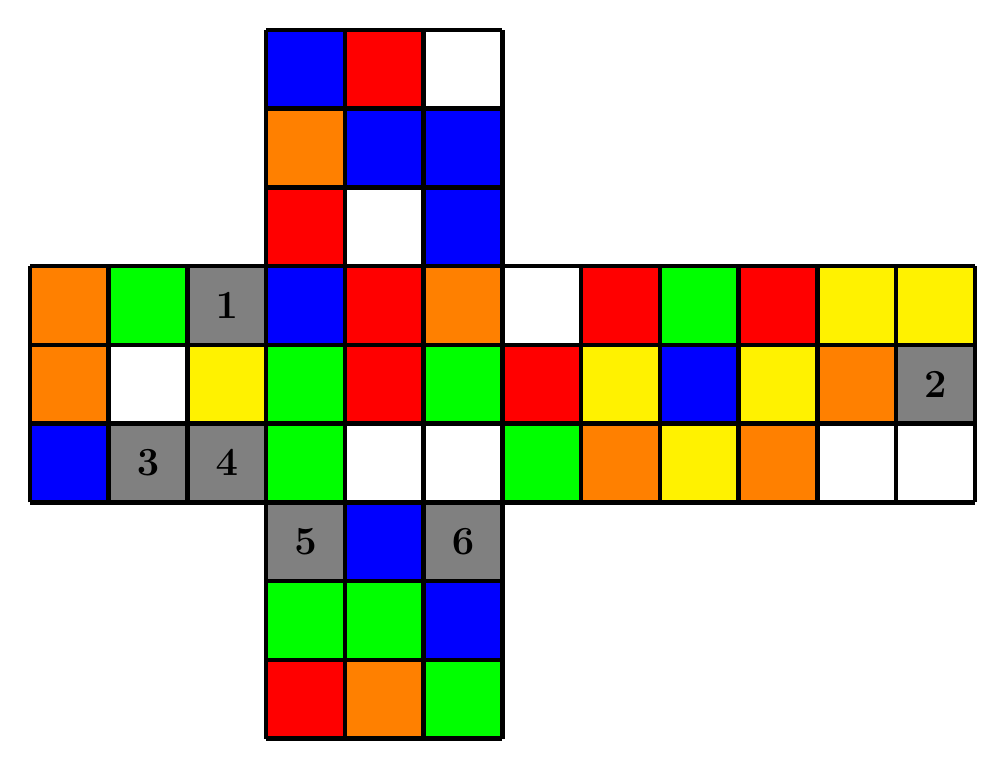
\begin{tikzpicture}[every node/.style={minimum size=1cm-\pgflinewidth, outer sep=0pt}]
\node[fill=blue] at (0.5,5.5) {};
\node[fill=red] at (1.5,5.5) {};
\node[fill=white] at (2.5,5.5) {};
\node[fill=orange] at (0.5,4.5) {};
\node[fill=blue] at (1.5,4.5) {};
\node[fill=blue] at (2.5,4.5) {};
\node[fill=red] at (0.5,3.5) {};
\node[fill=white] at (1.5,3.5) {};
\node[fill=blue] at (2.5,3.5) {};

\node[fill=orange] at (-2.5,2.5) {};
\node[fill=green] at (-1.5,2.5) {};
\node[fill=gray] at (-0.5,2.5) {\Large \textbf 1};
\node[fill=blue] at (0.5,2.5) {};
\node[fill=red] at (1.5,2.5) {};
\node[fill=orange] at (2.5,2.5) {};
\node[fill=white] at (3.5,2.5) {};
\node[fill=red] at (4.5,2.5) {};
\node[fill=green] at (5.5,2.5) {};
\node[fill=red] at (6.5,2.5) {};
\node[fill=yellow] at (7.5,2.5) {};
\node[fill=yellow] at (8.5,2.5) {};

\node[fill=orange] at (-2.5,1.5) {};
\node[fill=white] at (-1.5,1.5) {};
\node[fill=yellow] at (-0.5,1.5) {};
\node[fill=green] at (0.5,1.5) {};
\node[fill=red] at (1.5,1.5) {};
\node[fill=green] at (2.5,1.5) {};
\node[fill=red] at (3.5,1.5) {};
\node[fill=yellow] at (4.5,1.5) {};
\node[fill=blue] at (5.5,1.5) {};
\node[fill=yellow] at (6.5,1.5) {};
\node[fill=orange] at (7.5,1.5) {};
\node[fill=gray] at (8.5,1.5) {\Large \textbf 2};

\node[fill=blue] at (-2.5,0.5) {};
\node[fill=gray] at (-1.5,0.5) {\Large \textbf 3};
\node[fill=gray] at (-0.5,0.5) {\Large \textbf 4};
\node[fill=green] at (0.5,0.5) {};
\node[fill=white] at (1.5,0.5) {};
\node[fill=white] at (2.5,0.5) {};
\node[fill=green] at (3.5,0.5) {};
\node[fill=orange] at (4.5,0.5) {};
\node[fill=yellow] at (5.5,0.5) {};
\node[fill=orange] at (6.5,0.5) {};
\node[fill=white] at (7.5,0.5) {};
\node[fill=white] at (8.5,0.5) {};

\node[fill=gray] at (0.5,-0.5) {\Large \textbf 5};
\node[fill=blue] at (1.5,-0.5) {};
\node[fill=gray] at (2.5,-0.5) {\Large \textbf 6};
\node[fill=green] at (0.5,-1.5) {};
\node[fill=green] at (1.5,-1.5) {};
\node[fill=blue] at (2.5,-1.5) {};
\node[fill=red] at (0.5,-2.5) {};
\node[fill=orange] at (1.5,-2.5) {};
\node[fill=green] at (2.5,-2.5) {};

\draw[step=1cm,color=black, ultra thick] (-3,0) grid (9,3);
\draw[step=1cm,color=black, ultra thick] (0,-3) grid (3,0);
\draw[step=1cm,color=black, ultra thick] (0,3) grid (3,6);    
\end{tikzpicture}
\vspace{0.1cm}
\\
\noindent\normalsize \newtime  \textbf{Solution 20: U' B2 L2 U2 B L2 B U2 R2 D2 F U2 F' R B2 L D' F' U2 F' R' Fw}
\vspace{1cm}



{\noindent\Large \textbf{No. 21\qquad Difficulty:$\bigstar\bigstar$}}
\vspace{0.2cm}\\
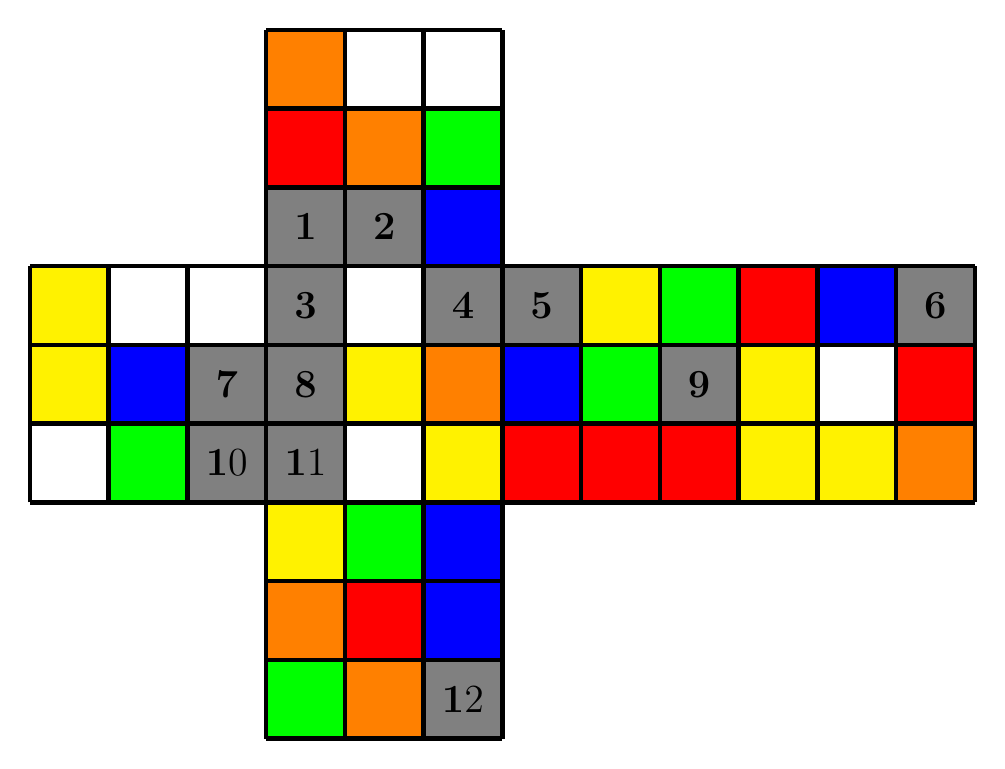
\begin{tikzpicture}[every node/.style={minimum size=1cm-\pgflinewidth, outer sep=0pt}]
\node[fill=orange] at (0.5,5.5) {};
\node[fill=white] at (1.5,5.5) {};
\node[fill=white] at (2.5,5.5) {};
\node[fill=red] at (0.5,4.5) {};
\node[fill=orange] at (1.5,4.5) {};
\node[fill=green] at (2.5,4.5) {};
\node[fill=gray] at (0.5,3.5) {\Large \textbf 1};
\node[fill=gray] at (1.5,3.5) {\Large \textbf 2};
\node[fill=blue] at (2.5,3.5) {};

\node[fill=yellow] at (-2.5,2.5) {};
\node[fill=white] at (-1.5,2.5) {};
\node[fill=white] at (-0.5,2.5) {};
\node[fill=gray] at (0.5,2.5) {\Large \textbf 3};
\node[fill=white] at (1.5,2.5) {};
\node[fill=gray] at (2.5,2.5) {\Large \textbf 4};
\node[fill=gray] at (3.5,2.5) {\Large \textbf 5};
\node[fill=yellow] at (4.5,2.5) {};
\node[fill=green] at (5.5,2.5) {};
\node[fill=red] at (6.5,2.5) {};
\node[fill=blue] at (7.5,2.5) {};
\node[fill=gray] at (8.5,2.5) {\Large \textbf 6};

\node[fill=yellow] at (-2.5,1.5) {};
\node[fill=blue] at (-1.5,1.5) {};
\node[fill=gray] at (-0.5,1.5) {\Large \textbf 7};
\node[fill=gray] at (0.5,1.5) {\Large \textbf 8};
\node[fill=yellow] at (1.5,1.5) {};
\node[fill=orange] at (2.5,1.5) {};
\node[fill=blue] at (3.5,1.5) {};
\node[fill=green] at (4.5,1.5) {};
\node[fill=gray] at (5.5,1.5) {\Large \textbf 9};
\node[fill=yellow] at (6.5,1.5) {};
\node[fill=white] at (7.5,1.5) {};
\node[fill=red] at (8.5,1.5) {};

\node[fill=white] at (-2.5,0.5) {};
\node[fill=green] at (-1.5,0.5) {};
\node[fill=gray] at (-0.5,0.5) {\Large \textbf 10};
\node[fill=gray] at (0.5,0.5) {\Large \textbf 11};
\node[fill=white] at (1.5,0.5) {};
\node[fill=yellow] at (2.5,0.5) {};
\node[fill=red] at (3.5,0.5) {};
\node[fill=red] at (4.5,0.5) {};
\node[fill=red] at (5.5,0.5) {};
\node[fill=yellow] at (6.5,0.5) {};
\node[fill=yellow] at (7.5,0.5) {};
\node[fill=orange] at (8.5,0.5) {};

\node[fill=yellow] at (0.5,-0.5) {};
\node[fill=green] at (1.5,-0.5) {};
\node[fill=blue] at (2.5,-0.5) {};
\node[fill=orange] at (0.5,-1.5) {};
\node[fill=red] at (1.5,-1.5) {};
\node[fill=blue] at (2.5,-1.5) {};
\node[fill=green] at (0.5,-2.5) {};
\node[fill=orange] at (1.5,-2.5) {};
\node[fill=gray] at (2.5,-2.5) {\Large \textbf 12};

\draw[step=1cm,color=black, ultra thick] (-3,0) grid (9,3);
\draw[step=1cm,color=black, ultra thick] (0,-3) grid (3,0);
\draw[step=1cm,color=black, ultra thick] (0,3) grid (3,6);    
\end{tikzpicture}
\vspace{0.1cm}
\\
\noindent\normalsize \newtime  \textbf{Solution 21: D R2 D F2 L2 U B2 U L2 U B2 U F' U' R U2 R2 D' L2 B' L Rw'}
\vspace{1cm}



{\noindent\Large \textbf{No. 22\qquad Difficulty:$\bigstar\bigstar$}}
\vspace{0.2cm}\\
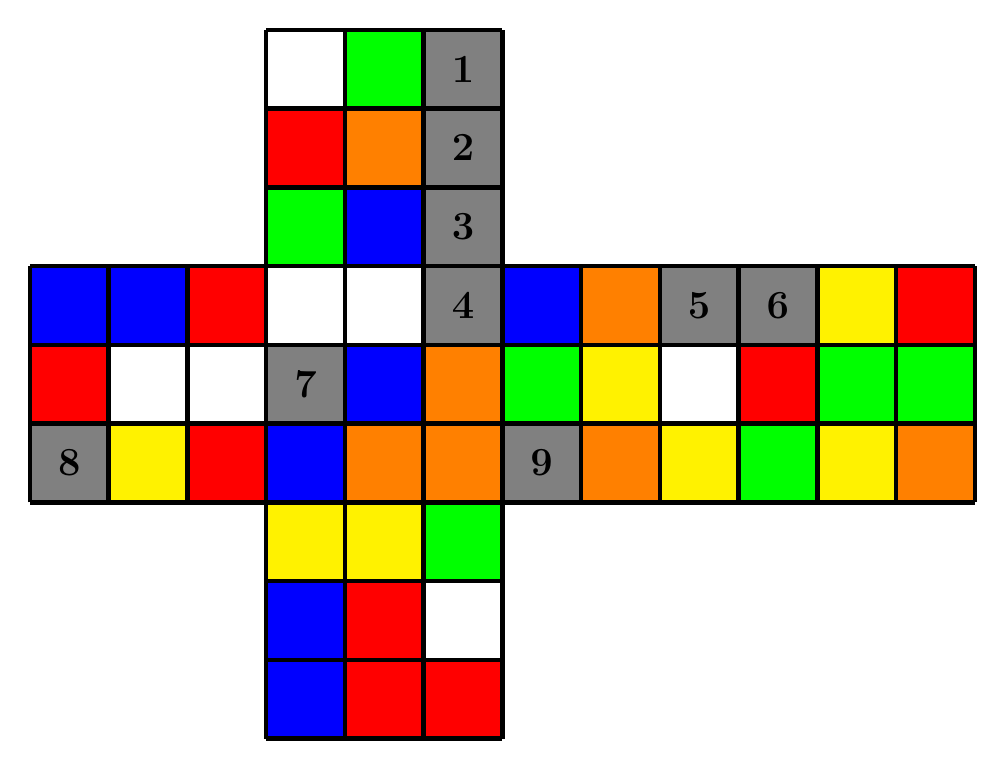
\begin{tikzpicture}[every node/.style={minimum size=1cm-\pgflinewidth, outer sep=0pt}]
\node[fill=white] at (0.5,5.5) {};
\node[fill=green] at (1.5,5.5) {};
\node[fill=gray] at (2.5,5.5) {\Large \textbf 1};
\node[fill=red] at (0.5,4.5) {};
\node[fill=orange] at (1.5,4.5) {};
\node[fill=gray] at (2.5,4.5) {\Large \textbf 2};
\node[fill=green] at (0.5,3.5) {};
\node[fill=blue] at (1.5,3.5) {};
\node[fill=gray] at (2.5,3.5) {\Large \textbf 3};

\node[fill=blue] at (-2.5,2.5) {};
\node[fill=blue] at (-1.5,2.5) {};
\node[fill=red] at (-0.5,2.5) {};
\node[fill=white] at (0.5,2.5) {};
\node[fill=white] at (1.5,2.5) {};
\node[fill=gray] at (2.5,2.5) {\Large \textbf 4};
\node[fill=blue] at (3.5,2.5) {};
\node[fill=orange] at (4.5,2.5) {};
\node[fill=gray] at (5.5,2.5) {\Large \textbf 5};
\node[fill=gray] at (6.5,2.5) {\Large \textbf 6};
\node[fill=yellow] at (7.5,2.5) {};
\node[fill=red] at (8.5,2.5) {};

\node[fill=red] at (-2.5,1.5) {};
\node[fill=white] at (-1.5,1.5) {};
\node[fill=white] at (-0.5,1.5) {};
\node[fill=gray] at (0.5,1.5) {\Large \textbf 7};
\node[fill=blue] at (1.5,1.5) {};
\node[fill=orange] at (2.5,1.5) {};
\node[fill=green] at (3.5,1.5) {};
\node[fill=yellow] at (4.5,1.5) {};
\node[fill=white] at (5.5,1.5) {};
\node[fill=red] at (6.5,1.5) {};
\node[fill=green] at (7.5,1.5) {};
\node[fill=green] at (8.5,1.5) {};

\node[fill=gray] at (-2.5,0.5) {\Large \textbf 8};
\node[fill=yellow] at (-1.5,0.5) {};
\node[fill=red] at (-0.5,0.5) {};
\node[fill=blue] at (0.5,0.5) {};
\node[fill=orange] at (1.5,0.5) {};
\node[fill=orange] at (2.5,0.5) {};
\node[fill=gray] at (3.5,0.5) {\Large \textbf 9};
\node[fill=orange] at (4.5,0.5) {};
\node[fill=yellow] at (5.5,0.5) {};
\node[fill=green] at (6.5,0.5) {};
\node[fill=yellow] at (7.5,0.5) {};
\node[fill=orange] at (8.5,0.5) {};

\node[fill=yellow] at (0.5,-0.5) {};
\node[fill=yellow] at (1.5,-0.5) {};
\node[fill=green] at (2.5,-0.5) {};
\node[fill=blue] at (0.5,-1.5) {};
\node[fill=red] at (1.5,-1.5) {};
\node[fill=white] at (2.5,-1.5) {};
\node[fill=blue] at (0.5,-2.5) {};
\node[fill=red] at (1.5,-2.5) {};
\node[fill=red] at (2.5,-2.5) {};

\draw[step=1cm,color=black, ultra thick] (-3,0) grid (9,3);
\draw[step=1cm,color=black, ultra thick] (0,-3) grid (3,0);
\draw[step=1cm,color=black, ultra thick] (0,3) grid (3,6);    
\end{tikzpicture}
\vspace{0.1cm}
\\
\noindent\normalsize \newtime  \textbf{Solution 22: F2 R2 D R2 U L2 U' F2 D' U2 R2 F' U' L' R' D B' D F2 U' Rw' Uw'}
\vspace{1cm}



{\noindent\Large \textbf{No. 23\qquad Difficulty:$\bigstar\bigstar$}}
\vspace{0.2cm}\\
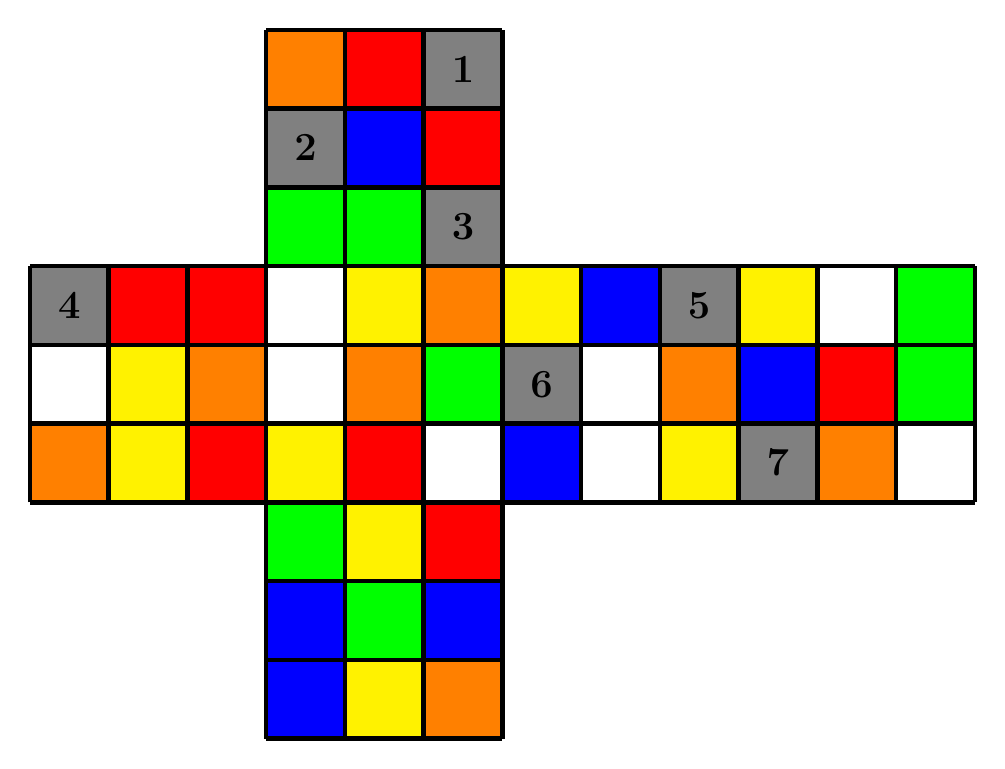
\begin{tikzpicture}[every node/.style={minimum size=1cm-\pgflinewidth, outer sep=0pt}]
\node[fill=orange] at (0.5,5.5) {};
\node[fill=red] at (1.5,5.5) {};
\node[fill=gray] at (2.5,5.5) {\Large \textbf 1};
\node[fill=gray] at (0.5,4.5) {\Large \textbf 2};
\node[fill=blue] at (1.5,4.5) {};
\node[fill=red] at (2.5,4.5) {};
\node[fill=green] at (0.5,3.5) {};
\node[fill=green] at (1.5,3.5) {};
\node[fill=gray] at (2.5,3.5) {\Large \textbf 3};

\node[fill=gray] at (-2.5,2.5) {\Large \textbf 4};
\node[fill=red] at (-1.5,2.5) {};
\node[fill=red] at (-0.5,2.5) {};
\node[fill=white] at (0.5,2.5) {};
\node[fill=yellow] at (1.5,2.5) {};
\node[fill=orange] at (2.5,2.5) {};
\node[fill=yellow] at (3.5,2.5) {};
\node[fill=blue] at (4.5,2.5) {};
\node[fill=gray] at (5.5,2.5) {\Large \textbf 5};
\node[fill=yellow] at (6.5,2.5) {};
\node[fill=white] at (7.5,2.5) {};
\node[fill=green] at (8.5,2.5) {};

\node[fill=white] at (-2.5,1.5) {};
\node[fill=yellow] at (-1.5,1.5) {};
\node[fill=orange] at (-0.5,1.5) {};
\node[fill=white] at (0.5,1.5) {};
\node[fill=orange] at (1.5,1.5) {};
\node[fill=green] at (2.5,1.5) {};
\node[fill=gray] at (3.5,1.5) {\Large \textbf 6};
\node[fill=white] at (4.5,1.5) {};
\node[fill=orange] at (5.5,1.5) {};
\node[fill=blue] at (6.5,1.5) {};
\node[fill=red] at (7.5,1.5) {};
\node[fill=green] at (8.5,1.5) {};

\node[fill=orange] at (-2.5,0.5) {};
\node[fill=yellow] at (-1.5,0.5) {};
\node[fill=red] at (-0.5,0.5) {};
\node[fill=yellow] at (0.5,0.5) {};
\node[fill=red] at (1.5,0.5) {};
\node[fill=white] at (2.5,0.5) {};
\node[fill=blue] at (3.5,0.5) {};
\node[fill=white] at (4.5,0.5) {};
\node[fill=yellow] at (5.5,0.5) {};
\node[fill=gray] at (6.5,0.5) {\Large \textbf 7};
\node[fill=orange] at (7.5,0.5) {};
\node[fill=white] at (8.5,0.5) {};

\node[fill=green] at (0.5,-0.5) {};
\node[fill=yellow] at (1.5,-0.5) {};
\node[fill=red] at (2.5,-0.5) {};
\node[fill=blue] at (0.5,-1.5) {};
\node[fill=green] at (1.5,-1.5) {};
\node[fill=blue] at (2.5,-1.5) {};
\node[fill=blue] at (0.5,-2.5) {};
\node[fill=yellow] at (1.5,-2.5) {};
\node[fill=orange] at (2.5,-2.5) {};

\draw[step=1cm,color=black, ultra thick] (-3,0) grid (9,3);
\draw[step=1cm,color=black, ultra thick] (0,-3) grid (3,0);
\draw[step=1cm,color=black, ultra thick] (0,3) grid (3,6);    
\end{tikzpicture}
\vspace{0.1cm}
\\
\noindent\normalsize \newtime  \textbf{Solution 23: B2 R2 D2 B2 D2 F2 R2 F2 U' L2 U' L' F2 D' B' F2 D2 R' D' R' Fw Uw2}
\vspace{1cm}



{\noindent\Large \textbf{No. 24\qquad Difficulty:$\bigstar\bigstar$}}
\vspace{0.2cm}\\
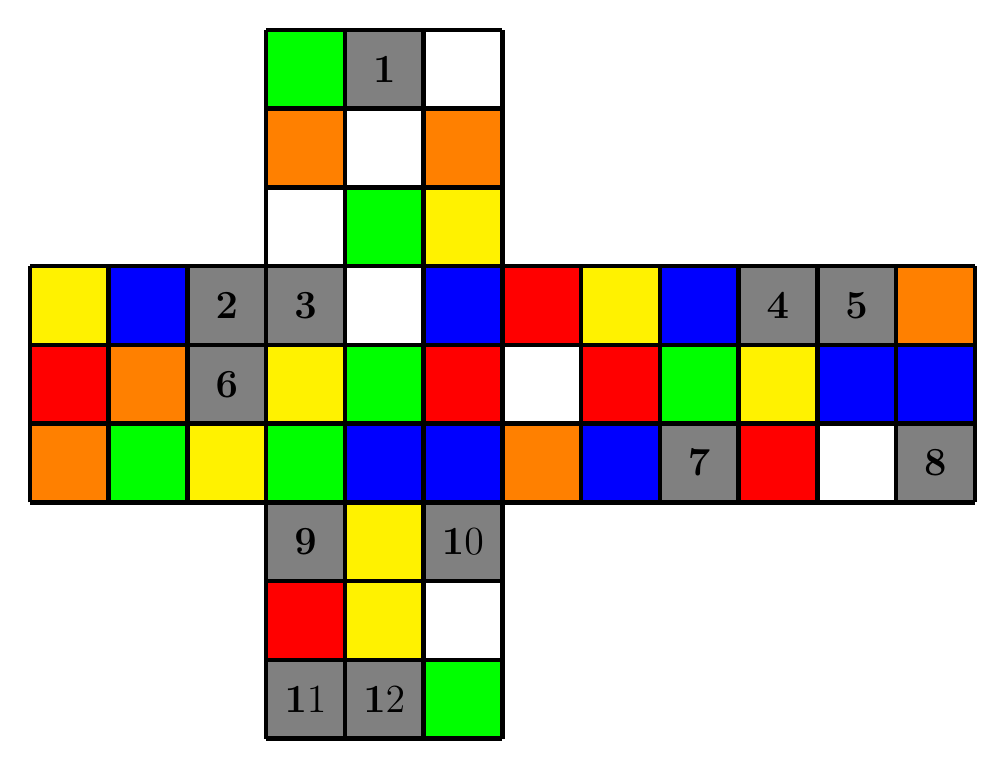
\begin{tikzpicture}[every node/.style={minimum size=1cm-\pgflinewidth, outer sep=0pt}]
\node[fill=green] at (0.5,5.5) {};
\node[fill=gray] at (1.5,5.5) {\Large \textbf 1};
\node[fill=white] at (2.5,5.5) {};
\node[fill=orange] at (0.5,4.5) {};
\node[fill=white] at (1.5,4.5) {};
\node[fill=orange] at (2.5,4.5) {};
\node[fill=white] at (0.5,3.5) {};
\node[fill=green] at (1.5,3.5) {};
\node[fill=yellow] at (2.5,3.5) {};

\node[fill=yellow] at (-2.5,2.5) {};
\node[fill=blue] at (-1.5,2.5) {};
\node[fill=gray] at (-0.5,2.5) {\Large \textbf 2};
\node[fill=gray] at (0.5,2.5) {\Large \textbf 3};
\node[fill=white] at (1.5,2.5) {};
\node[fill=blue] at (2.5,2.5) {};
\node[fill=red] at (3.5,2.5) {};
\node[fill=yellow] at (4.5,2.5) {};
\node[fill=blue] at (5.5,2.5) {};
\node[fill=gray] at (6.5,2.5) {\Large \textbf 4};
\node[fill=gray] at (7.5,2.5) {\Large \textbf 5};
\node[fill=orange] at (8.5,2.5) {};

\node[fill=red] at (-2.5,1.5) {};
\node[fill=orange] at (-1.5,1.5) {};
\node[fill=gray] at (-0.5,1.5) {\Large \textbf 6};
\node[fill=yellow] at (0.5,1.5) {};
\node[fill=green] at (1.5,1.5) {};
\node[fill=red] at (2.5,1.5) {};
\node[fill=white] at (3.5,1.5) {};
\node[fill=red] at (4.5,1.5) {};
\node[fill=green] at (5.5,1.5) {};
\node[fill=yellow] at (6.5,1.5) {};
\node[fill=blue] at (7.5,1.5) {};
\node[fill=blue] at (8.5,1.5) {};

\node[fill=orange] at (-2.5,0.5) {};
\node[fill=green] at (-1.5,0.5) {};
\node[fill=yellow] at (-0.5,0.5) {};
\node[fill=green] at (0.5,0.5) {};
\node[fill=blue] at (1.5,0.5) {};
\node[fill=blue] at (2.5,0.5) {};
\node[fill=orange] at (3.5,0.5) {};
\node[fill=blue] at (4.5,0.5) {};
\node[fill=gray] at (5.5,0.5) {\Large \textbf 7};
\node[fill=red] at (6.5,0.5) {};
\node[fill=white] at (7.5,0.5) {};
\node[fill=gray] at (8.5,0.5) {\Large \textbf 8};

\node[fill=gray] at (0.5,-0.5) {\Large \textbf 9};
\node[fill=yellow] at (1.5,-0.5) {};
\node[fill=gray] at (2.5,-0.5) {\Large \textbf 10};
\node[fill=red] at (0.5,-1.5) {};
\node[fill=yellow] at (1.5,-1.5) {};
\node[fill=white] at (2.5,-1.5) {};
\node[fill=gray] at (0.5,-2.5) {\Large \textbf 11};
\node[fill=gray] at (1.5,-2.5) {\Large \textbf 12};
\node[fill=green] at (2.5,-2.5) {};

\draw[step=1cm,color=black, ultra thick] (-3,0) grid (9,3);
\draw[step=1cm,color=black, ultra thick] (0,-3) grid (3,0);
\draw[step=1cm,color=black, ultra thick] (0,3) grid (3,6);    
\end{tikzpicture}
\vspace{0.1cm}
\\
\noindent\normalsize \newtime  \textbf{Solution 24: B R D2 F2 R2 F' U D L D L2 U F2 U' R2 F2 B2 U B2 D R2 Rw2 Uw}
\vspace{1cm}



{\noindent\Large \textbf{No. 25\qquad Difficulty:$\bigstar\bigstar$}}
\vspace{0.2cm}\\
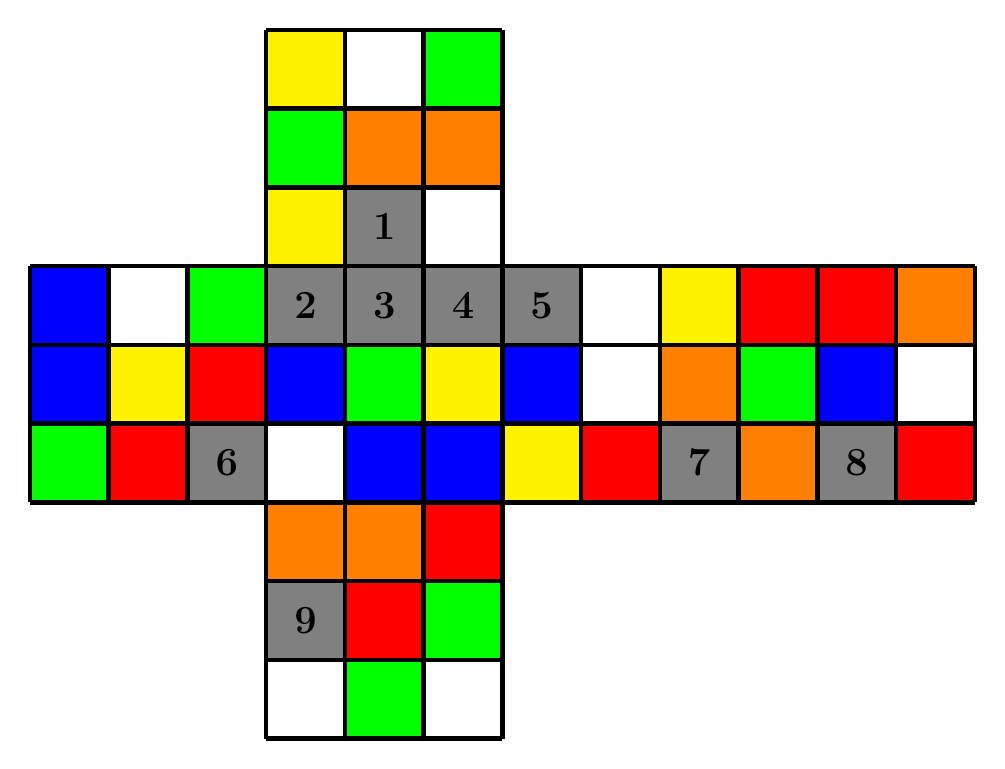
\begin{tikzpicture}[every node/.style={minimum size=1cm-\pgflinewidth, outer sep=0pt}]
\node[fill=yellow] at (0.5,5.5) {};
\node[fill=white] at (1.5,5.5) {};
\node[fill=green] at (2.5,5.5) {};
\node[fill=green] at (0.5,4.5) {};
\node[fill=orange] at (1.5,4.5) {};
\node[fill=orange] at (2.5,4.5) {};
\node[fill=yellow] at (0.5,3.5) {};
\node[fill=gray] at (1.5,3.5) {\Large \textbf 1};
\node[fill=white] at (2.5,3.5) {};

\node[fill=blue] at (-2.5,2.5) {};
\node[fill=white] at (-1.5,2.5) {};
\node[fill=green] at (-0.5,2.5) {};
\node[fill=gray] at (0.5,2.5) {\Large \textbf 2};
\node[fill=gray] at (1.5,2.5) {\Large \textbf 3};
\node[fill=gray] at (2.5,2.5) {\Large \textbf 4};
\node[fill=gray] at (3.5,2.5) {\Large \textbf 5};
\node[fill=white] at (4.5,2.5) {};
\node[fill=yellow] at (5.5,2.5) {};
\node[fill=red] at (6.5,2.5) {};
\node[fill=red] at (7.5,2.5) {};
\node[fill=orange] at (8.5,2.5) {};

\node[fill=blue] at (-2.5,1.5) {};
\node[fill=yellow] at (-1.5,1.5) {};
\node[fill=red] at (-0.5,1.5) {};
\node[fill=blue] at (0.5,1.5) {};
\node[fill=green] at (1.5,1.5) {};
\node[fill=yellow] at (2.5,1.5) {};
\node[fill=blue] at (3.5,1.5) {};
\node[fill=white] at (4.5,1.5) {};
\node[fill=orange] at (5.5,1.5) {};
\node[fill=green] at (6.5,1.5) {};
\node[fill=blue] at (7.5,1.5) {};
\node[fill=white] at (8.5,1.5) {};

\node[fill=green] at (-2.5,0.5) {};
\node[fill=red] at (-1.5,0.5) {};
\node[fill=gray] at (-0.5,0.5) {\Large \textbf 6};
\node[fill=white] at (0.5,0.5) {};
\node[fill=blue] at (1.5,0.5) {};
\node[fill=blue] at (2.5,0.5) {};
\node[fill=yellow] at (3.5,0.5) {};
\node[fill=red] at (4.5,0.5) {};
\node[fill=gray] at (5.5,0.5) {\Large \textbf 7};
\node[fill=orange] at (6.5,0.5) {};
\node[fill=gray] at (7.5,0.5) {\Large \textbf 8};
\node[fill=red] at (8.5,0.5) {};

\node[fill=orange] at (0.5,-0.5) {};
\node[fill=orange] at (1.5,-0.5) {};
\node[fill=red] at (2.5,-0.5) {};
\node[fill=gray] at (0.5,-1.5) {\Large \textbf 9};
\node[fill=red] at (1.5,-1.5) {};
\node[fill=green] at (2.5,-1.5) {};
\node[fill=white] at (0.5,-2.5) {};
\node[fill=green] at (1.5,-2.5) {};
\node[fill=white] at (2.5,-2.5) {};

\draw[step=1cm,color=black, ultra thick] (-3,0) grid (9,3);
\draw[step=1cm,color=black, ultra thick] (0,-3) grid (3,0);
\draw[step=1cm,color=black, ultra thick] (0,3) grid (3,6);    
\end{tikzpicture}
\vspace{0.1cm}
\\
\noindent\normalsize \newtime  \textbf{Solution 25: F2 D L2 D R2 B2 U2 L2 D2 L2 U B' D U2 R2 D2 B2 F R Rw' Uw}
\vspace{1cm}



{\noindent\Large \textbf{No. 26\qquad Difficulty:$\bigstar\bigstar$}}
\vspace{0.2cm}\\
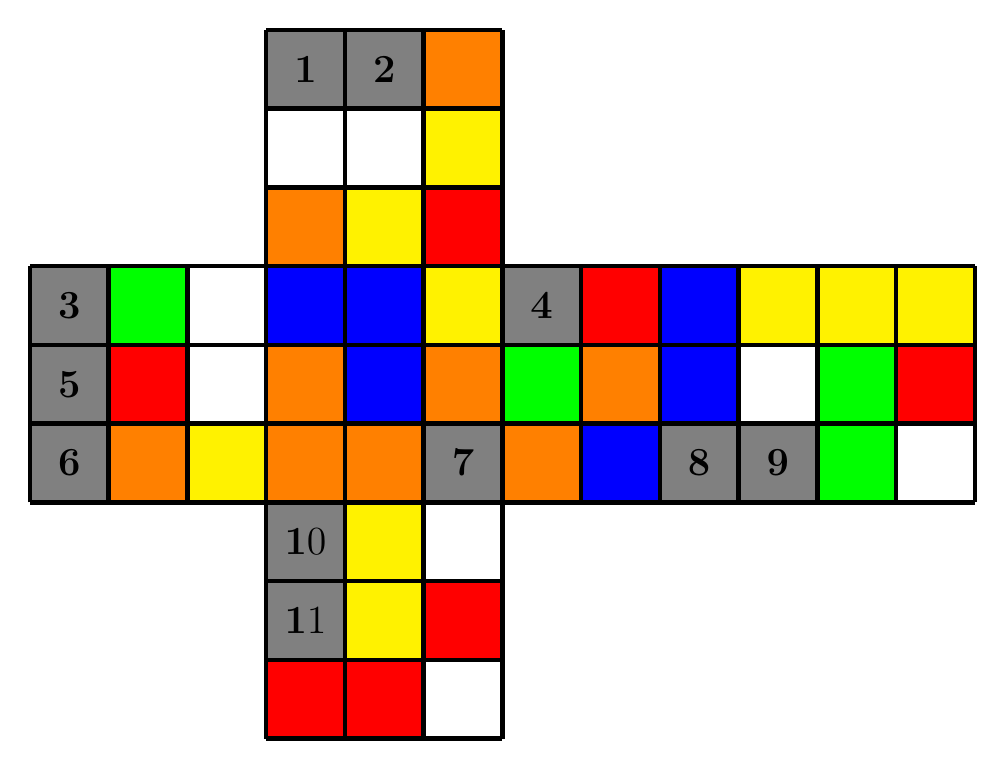
\begin{tikzpicture}[every node/.style={minimum size=1cm-\pgflinewidth, outer sep=0pt}]
\node[fill=gray] at (0.5,5.5) {\Large \textbf 1};
\node[fill=gray] at (1.5,5.5) {\Large \textbf 2};
\node[fill=orange] at (2.5,5.5) {};
\node[fill=white] at (0.5,4.5) {};
\node[fill=white] at (1.5,4.5) {};
\node[fill=yellow] at (2.5,4.5) {};
\node[fill=orange] at (0.5,3.5) {};
\node[fill=yellow] at (1.5,3.5) {};
\node[fill=red] at (2.5,3.5) {};

\node[fill=gray] at (-2.5,2.5) {\Large \textbf 3};
\node[fill=green] at (-1.5,2.5) {};
\node[fill=white] at (-0.5,2.5) {};
\node[fill=blue] at (0.5,2.5) {};
\node[fill=blue] at (1.5,2.5) {};
\node[fill=yellow] at (2.5,2.5) {};
\node[fill=gray] at (3.5,2.5) {\Large \textbf 4};
\node[fill=red] at (4.5,2.5) {};
\node[fill=blue] at (5.5,2.5) {};
\node[fill=yellow] at (6.5,2.5) {};
\node[fill=yellow] at (7.5,2.5) {};
\node[fill=yellow] at (8.5,2.5) {};

\node[fill=gray] at (-2.5,1.5) {\Large \textbf 5};
\node[fill=red] at (-1.5,1.5) {};
\node[fill=white] at (-0.5,1.5) {};
\node[fill=orange] at (0.5,1.5) {};
\node[fill=blue] at (1.5,1.5) {};
\node[fill=orange] at (2.5,1.5) {};
\node[fill=green] at (3.5,1.5) {};
\node[fill=orange] at (4.5,1.5) {};
\node[fill=blue] at (5.5,1.5) {};
\node[fill=white] at (6.5,1.5) {};
\node[fill=green] at (7.5,1.5) {};
\node[fill=red] at (8.5,1.5) {};

\node[fill=gray] at (-2.5,0.5) {\Large \textbf 6};
\node[fill=orange] at (-1.5,0.5) {};
\node[fill=yellow] at (-0.5,0.5) {};
\node[fill=orange] at (0.5,0.5) {};
\node[fill=orange] at (1.5,0.5) {};
\node[fill=gray] at (2.5,0.5) {\Large \textbf 7};
\node[fill=orange] at (3.5,0.5) {};
\node[fill=blue] at (4.5,0.5) {};
\node[fill=gray] at (5.5,0.5) {\Large \textbf 8};
\node[fill=gray] at (6.5,0.5) {\Large \textbf 9};
\node[fill=green] at (7.5,0.5) {};
\node[fill=white] at (8.5,0.5) {};

\node[fill=gray] at (0.5,-0.5) {\Large \textbf 10};
\node[fill=yellow] at (1.5,-0.5) {};
\node[fill=white] at (2.5,-0.5) {};
\node[fill=gray] at (0.5,-1.5) {\Large \textbf 11};
\node[fill=yellow] at (1.5,-1.5) {};
\node[fill=red] at (2.5,-1.5) {};
\node[fill=red] at (0.5,-2.5) {};
\node[fill=red] at (1.5,-2.5) {};
\node[fill=white] at (2.5,-2.5) {};

\draw[step=1cm,color=black, ultra thick] (-3,0) grid (9,3);
\draw[step=1cm,color=black, ultra thick] (0,-3) grid (3,0);
\draw[step=1cm,color=black, ultra thick] (0,3) grid (3,6);    
\end{tikzpicture}
\vspace{0.1cm}
\\
\noindent\normalsize \newtime  \textbf{Solution 26: R2 D U2 B2 D' U' F2 U' F D R' U R2 F' L R2 U' Rw2 Uw'}
\vspace{1cm}



{\noindent\Large \textbf{No. 27\qquad Difficulty:$\bigstar\bigstar$}}
\vspace{0.2cm}\\
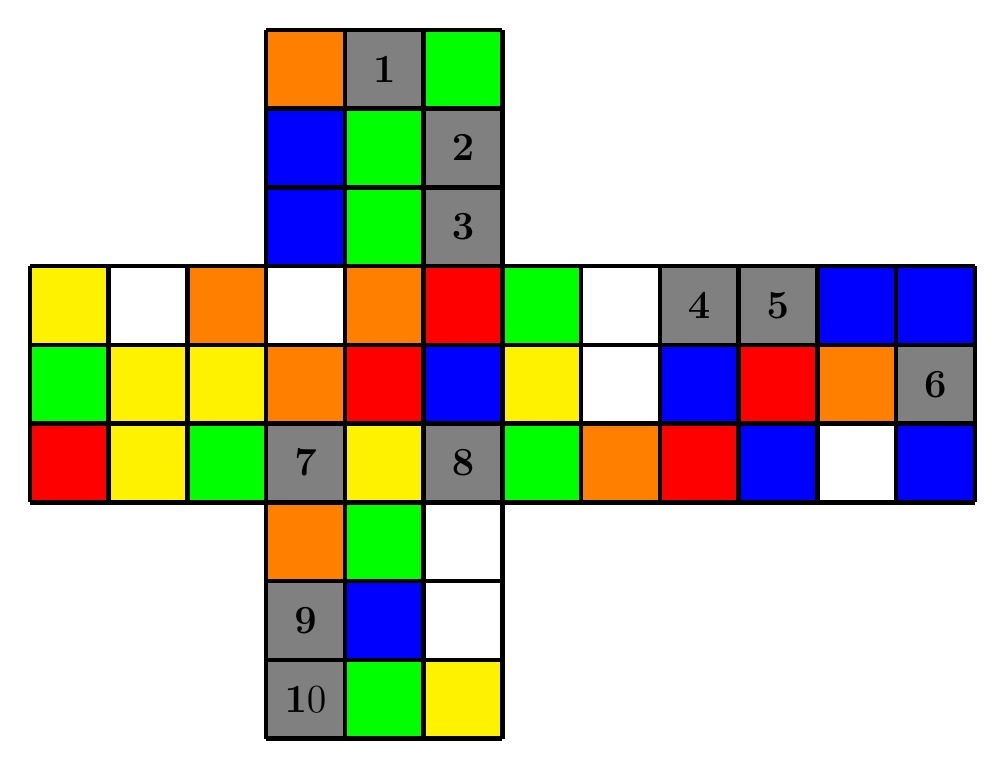
\begin{tikzpicture}[every node/.style={minimum size=1cm-\pgflinewidth, outer sep=0pt}]
\node[fill=orange] at (0.5,5.5) {};
\node[fill=gray] at (1.5,5.5) {\Large \textbf 1};
\node[fill=green] at (2.5,5.5) {};
\node[fill=blue] at (0.5,4.5) {};
\node[fill=green] at (1.5,4.5) {};
\node[fill=gray] at (2.5,4.5) {\Large \textbf 2};
\node[fill=blue] at (0.5,3.5) {};
\node[fill=green] at (1.5,3.5) {};
\node[fill=gray] at (2.5,3.5) {\Large \textbf 3};

\node[fill=yellow] at (-2.5,2.5) {};
\node[fill=white] at (-1.5,2.5) {};
\node[fill=orange] at (-0.5,2.5) {};
\node[fill=white] at (0.5,2.5) {};
\node[fill=orange] at (1.5,2.5) {};
\node[fill=red] at (2.5,2.5) {};
\node[fill=green] at (3.5,2.5) {};
\node[fill=white] at (4.5,2.5) {};
\node[fill=gray] at (5.5,2.5) {\Large \textbf 4};
\node[fill=gray] at (6.5,2.5) {\Large \textbf 5};
\node[fill=blue] at (7.5,2.5) {};
\node[fill=blue] at (8.5,2.5) {};

\node[fill=green] at (-2.5,1.5) {};
\node[fill=yellow] at (-1.5,1.5) {};
\node[fill=yellow] at (-0.5,1.5) {};
\node[fill=orange] at (0.5,1.5) {};
\node[fill=red] at (1.5,1.5) {};
\node[fill=blue] at (2.5,1.5) {};
\node[fill=yellow] at (3.5,1.5) {};
\node[fill=white] at (4.5,1.5) {};
\node[fill=blue] at (5.5,1.5) {};
\node[fill=red] at (6.5,1.5) {};
\node[fill=orange] at (7.5,1.5) {};
\node[fill=gray] at (8.5,1.5) {\Large \textbf 6};

\node[fill=red] at (-2.5,0.5) {};
\node[fill=yellow] at (-1.5,0.5) {};
\node[fill=green] at (-0.5,0.5) {};
\node[fill=gray] at (0.5,0.5) {\Large \textbf 7};
\node[fill=yellow] at (1.5,0.5) {};
\node[fill=gray] at (2.5,0.5) {\Large \textbf 8};
\node[fill=green] at (3.5,0.5) {};
\node[fill=orange] at (4.5,0.5) {};
\node[fill=red] at (5.5,0.5) {};
\node[fill=blue] at (6.5,0.5) {};
\node[fill=white] at (7.5,0.5) {};
\node[fill=blue] at (8.5,0.5) {};

\node[fill=orange] at (0.5,-0.5) {};
\node[fill=green] at (1.5,-0.5) {};
\node[fill=white] at (2.5,-0.5) {};
\node[fill=gray] at (0.5,-1.5) {\Large \textbf 9};
\node[fill=blue] at (1.5,-1.5) {};
\node[fill=white] at (2.5,-1.5) {};
\node[fill=gray] at (0.5,-2.5) {\Large \textbf 10};
\node[fill=green] at (1.5,-2.5) {};
\node[fill=yellow] at (2.5,-2.5) {};

\draw[step=1cm,color=black, ultra thick] (-3,0) grid (9,3);
\draw[step=1cm,color=black, ultra thick] (0,-3) grid (3,0);
\draw[step=1cm,color=black, ultra thick] (0,3) grid (3,6);    
\end{tikzpicture}
\vspace{0.1cm}
\\
\noindent\normalsize \newtime  \textbf{Solution 27: F' R2 D2 B' D2 L2 F2 D2 F' D2 B' R' F L2 D2 U' R2 F2 Fw'}
\vspace{1cm}



{\noindent\Large \textbf{No. 28\qquad Difficulty:$\bigstar\bigstar$}}
\vspace{0.2cm}\\
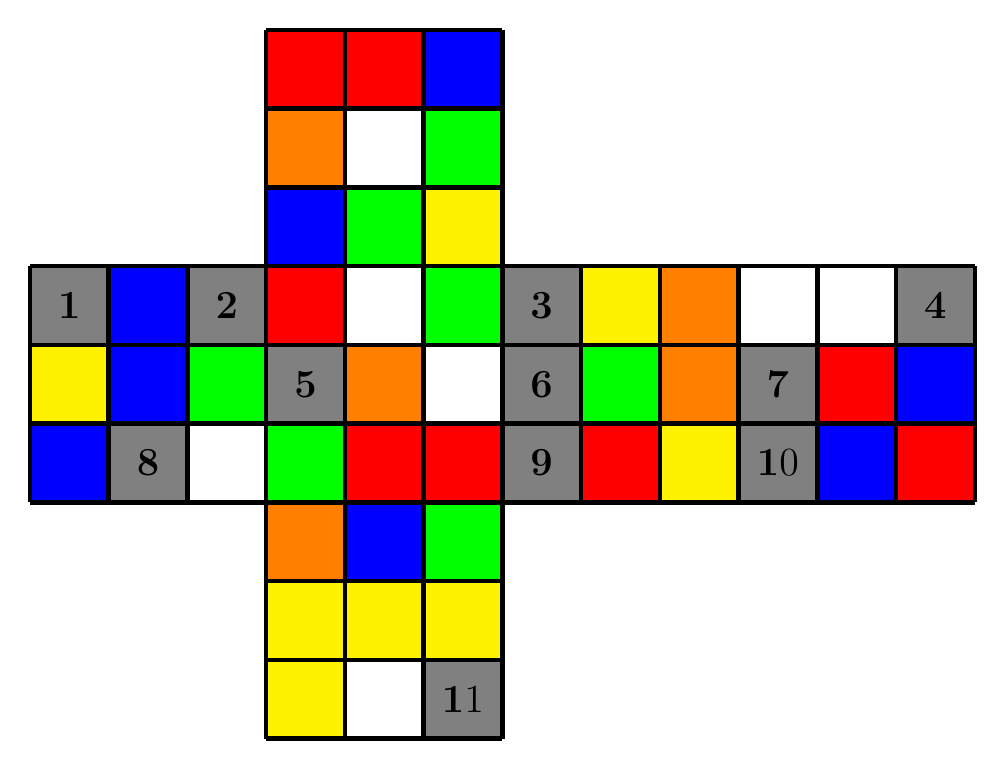
\begin{tikzpicture}[every node/.style={minimum size=1cm-\pgflinewidth, outer sep=0pt}]
\node[fill=red] at (0.5,5.5) {};
\node[fill=red] at (1.5,5.5) {};
\node[fill=blue] at (2.5,5.5) {};
\node[fill=orange] at (0.5,4.5) {};
\node[fill=white] at (1.5,4.5) {};
\node[fill=green] at (2.5,4.5) {};
\node[fill=blue] at (0.5,3.5) {};
\node[fill=green] at (1.5,3.5) {};
\node[fill=yellow] at (2.5,3.5) {};

\node[fill=gray] at (-2.5,2.5) {\Large \textbf 1};
\node[fill=blue] at (-1.5,2.5) {};
\node[fill=gray] at (-0.5,2.5) {\Large \textbf 2};
\node[fill=red] at (0.5,2.5) {};
\node[fill=white] at (1.5,2.5) {};
\node[fill=green] at (2.5,2.5) {};
\node[fill=gray] at (3.5,2.5) {\Large \textbf 3};
\node[fill=yellow] at (4.5,2.5) {};
\node[fill=orange] at (5.5,2.5) {};
\node[fill=white] at (6.5,2.5) {};
\node[fill=white] at (7.5,2.5) {};
\node[fill=gray] at (8.5,2.5) {\Large \textbf 4};

\node[fill=yellow] at (-2.5,1.5) {};
\node[fill=blue] at (-1.5,1.5) {};
\node[fill=green] at (-0.5,1.5) {};
\node[fill=gray] at (0.5,1.5) {\Large \textbf 5};
\node[fill=orange] at (1.5,1.5) {};
\node[fill=white] at (2.5,1.5) {};
\node[fill=gray] at (3.5,1.5) {\Large \textbf 6};
\node[fill=green] at (4.5,1.5) {};
\node[fill=orange] at (5.5,1.5) {};
\node[fill=gray] at (6.5,1.5) {\Large \textbf 7};
\node[fill=red] at (7.5,1.5) {};
\node[fill=blue] at (8.5,1.5) {};

\node[fill=blue] at (-2.5,0.5) {};
\node[fill=gray] at (-1.5,0.5) {\Large \textbf 8};
\node[fill=white] at (-0.5,0.5) {};
\node[fill=green] at (0.5,0.5) {};
\node[fill=red] at (1.5,0.5) {};
\node[fill=red] at (2.5,0.5) {};
\node[fill=gray] at (3.5,0.5) {\Large \textbf 9};
\node[fill=red] at (4.5,0.5) {};
\node[fill=yellow] at (5.5,0.5) {};
\node[fill=gray] at (6.5,0.5) {\Large \textbf 10};
\node[fill=blue] at (7.5,0.5) {};
\node[fill=red] at (8.5,0.5) {};

\node[fill=orange] at (0.5,-0.5) {};
\node[fill=blue] at (1.5,-0.5) {};
\node[fill=green] at (2.5,-0.5) {};
\node[fill=yellow] at (0.5,-1.5) {};
\node[fill=yellow] at (1.5,-1.5) {};
\node[fill=yellow] at (2.5,-1.5) {};
\node[fill=yellow] at (0.5,-2.5) {};
\node[fill=white] at (1.5,-2.5) {};
\node[fill=gray] at (2.5,-2.5) {\Large \textbf 11};

\draw[step=1cm,color=black, ultra thick] (-3,0) grid (9,3);
\draw[step=1cm,color=black, ultra thick] (0,-3) grid (3,0);
\draw[step=1cm,color=black, ultra thick] (0,3) grid (3,6);    
\end{tikzpicture}
\vspace{0.1cm}
\\
\noindent\normalsize \newtime  \textbf{Solution 28: F2 R B R2 U' B R B2 R2 B2 L2 U' L2 F2 U B2 U2 F2 D B D2 Rw2}
\vspace{1cm}



{\noindent\Large \textbf{No. 29\qquad Difficulty:$\bigstar\bigstar$}}
\vspace{0.2cm}\\
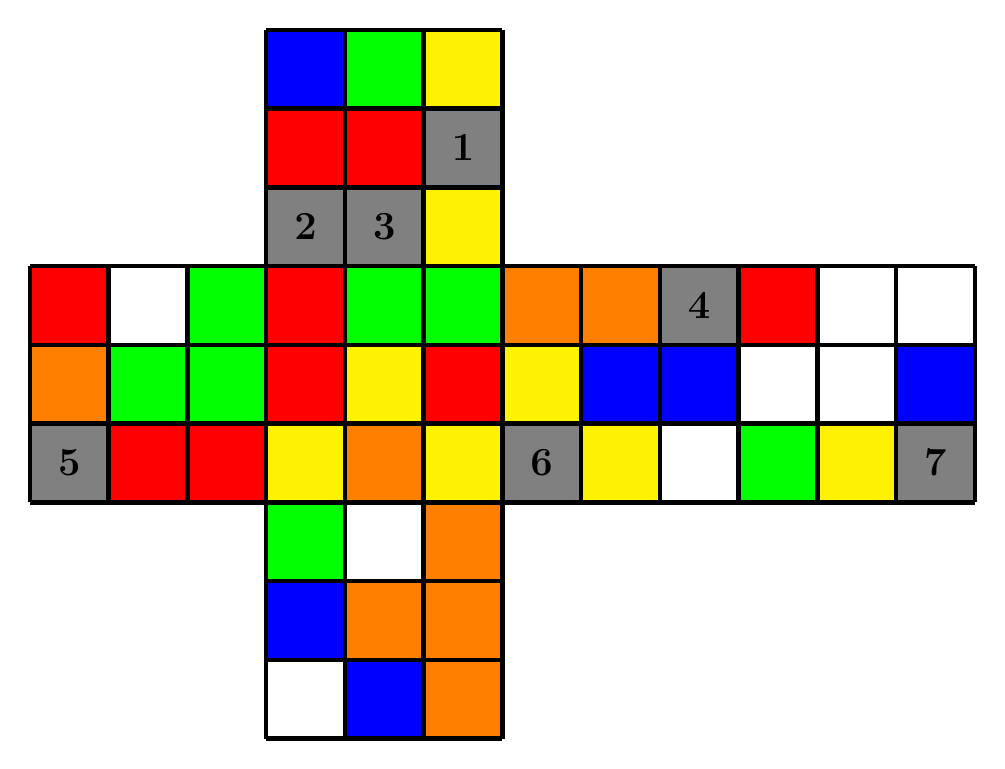
\begin{tikzpicture}[every node/.style={minimum size=1cm-\pgflinewidth, outer sep=0pt}]
\node[fill=blue] at (0.5,5.5) {};
\node[fill=green] at (1.5,5.5) {};
\node[fill=yellow] at (2.5,5.5) {};
\node[fill=red] at (0.5,4.5) {};
\node[fill=red] at (1.5,4.5) {};
\node[fill=gray] at (2.5,4.5) {\Large \textbf 1};
\node[fill=gray] at (0.5,3.5) {\Large \textbf 2};
\node[fill=gray] at (1.5,3.5) {\Large \textbf 3};
\node[fill=yellow] at (2.5,3.5) {};

\node[fill=red] at (-2.5,2.5) {};
\node[fill=white] at (-1.5,2.5) {};
\node[fill=green] at (-0.5,2.5) {};
\node[fill=red] at (0.5,2.5) {};
\node[fill=green] at (1.5,2.5) {};
\node[fill=green] at (2.5,2.5) {};
\node[fill=orange] at (3.5,2.5) {};
\node[fill=orange] at (4.5,2.5) {};
\node[fill=gray] at (5.5,2.5) {\Large \textbf 4};
\node[fill=red] at (6.5,2.5) {};
\node[fill=white] at (7.5,2.5) {};
\node[fill=white] at (8.5,2.5) {};

\node[fill=orange] at (-2.5,1.5) {};
\node[fill=green] at (-1.5,1.5) {};
\node[fill=green] at (-0.5,1.5) {};
\node[fill=red] at (0.5,1.5) {};
\node[fill=yellow] at (1.5,1.5) {};
\node[fill=red] at (2.5,1.5) {};
\node[fill=yellow] at (3.5,1.5) {};
\node[fill=blue] at (4.5,1.5) {};
\node[fill=blue] at (5.5,1.5) {};
\node[fill=white] at (6.5,1.5) {};
\node[fill=white] at (7.5,1.5) {};
\node[fill=blue] at (8.5,1.5) {};

\node[fill=gray] at (-2.5,0.5) {\Large \textbf 5};
\node[fill=red] at (-1.5,0.5) {};
\node[fill=red] at (-0.5,0.5) {};
\node[fill=yellow] at (0.5,0.5) {};
\node[fill=orange] at (1.5,0.5) {};
\node[fill=yellow] at (2.5,0.5) {};
\node[fill=gray] at (3.5,0.5) {\Large \textbf 6};
\node[fill=yellow] at (4.5,0.5) {};
\node[fill=white] at (5.5,0.5) {};
\node[fill=green] at (6.5,0.5) {};
\node[fill=yellow] at (7.5,0.5) {};
\node[fill=gray] at (8.5,0.5) {\Large \textbf 7};

\node[fill=green] at (0.5,-0.5) {};
\node[fill=white] at (1.5,-0.5) {};
\node[fill=orange] at (2.5,-0.5) {};
\node[fill=blue] at (0.5,-1.5) {};
\node[fill=orange] at (1.5,-1.5) {};
\node[fill=orange] at (2.5,-1.5) {};
\node[fill=white] at (0.5,-2.5) {};
\node[fill=blue] at (1.5,-2.5) {};
\node[fill=orange] at (2.5,-2.5) {};

\draw[step=1cm,color=black, ultra thick] (-3,0) grid (9,3);
\draw[step=1cm,color=black, ultra thick] (0,-3) grid (3,0);
\draw[step=1cm,color=black, ultra thick] (0,3) grid (3,6);    
\end{tikzpicture}
\vspace{0.1cm}
\\
\noindent\normalsize \newtime  \textbf{Solution 29: B' L2 D B2 L2 D' R2 D' B2 D B2 U L2 F R2 U' B' R D' B' F2 Rw Uw2}
\vspace{1cm}



{\noindent\Large \textbf{No. 30\qquad Difficulty:$\bigstar\bigstar$}}
\vspace{0.2cm}\\
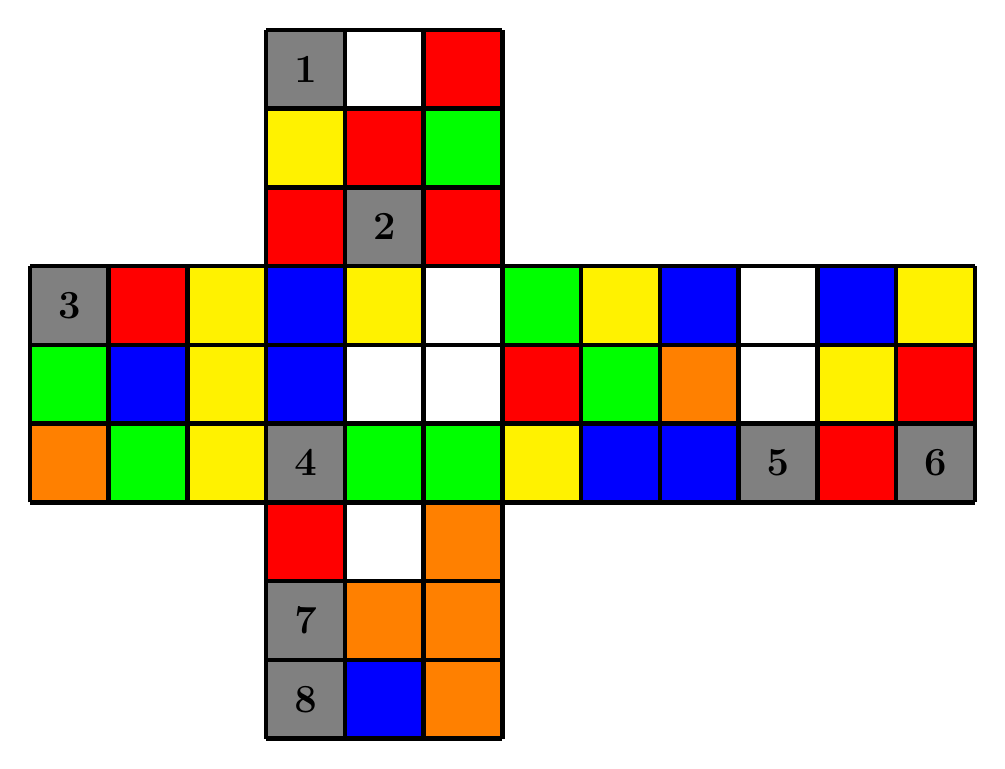
\begin{tikzpicture}[every node/.style={minimum size=1cm-\pgflinewidth, outer sep=0pt}]
\node[fill=gray] at (0.5,5.5) {\Large \textbf 1};
\node[fill=white] at (1.5,5.5) {};
\node[fill=red] at (2.5,5.5) {};
\node[fill=yellow] at (0.5,4.5) {};
\node[fill=red] at (1.5,4.5) {};
\node[fill=green] at (2.5,4.5) {};
\node[fill=red] at (0.5,3.5) {};
\node[fill=gray] at (1.5,3.5) {\Large \textbf 2};
\node[fill=red] at (2.5,3.5) {};

\node[fill=gray] at (-2.5,2.5) {\Large \textbf 3};
\node[fill=red] at (-1.5,2.5) {};
\node[fill=yellow] at (-0.5,2.5) {};
\node[fill=blue] at (0.5,2.5) {};
\node[fill=yellow] at (1.5,2.5) {};
\node[fill=white] at (2.5,2.5) {};
\node[fill=green] at (3.5,2.5) {};
\node[fill=yellow] at (4.5,2.5) {};
\node[fill=blue] at (5.5,2.5) {};
\node[fill=white] at (6.5,2.5) {};
\node[fill=blue] at (7.5,2.5) {};
\node[fill=yellow] at (8.5,2.5) {};

\node[fill=green] at (-2.5,1.5) {};
\node[fill=blue] at (-1.5,1.5) {};
\node[fill=yellow] at (-0.5,1.5) {};
\node[fill=blue] at (0.5,1.5) {};
\node[fill=white] at (1.5,1.5) {};
\node[fill=white] at (2.5,1.5) {};
\node[fill=red] at (3.5,1.5) {};
\node[fill=green] at (4.5,1.5) {};
\node[fill=orange] at (5.5,1.5) {};
\node[fill=white] at (6.5,1.5) {};
\node[fill=yellow] at (7.5,1.5) {};
\node[fill=red] at (8.5,1.5) {};

\node[fill=orange] at (-2.5,0.5) {};
\node[fill=green] at (-1.5,0.5) {};
\node[fill=yellow] at (-0.5,0.5) {};
\node[fill=gray] at (0.5,0.5) {\Large \textbf 4};
\node[fill=green] at (1.5,0.5) {};
\node[fill=green] at (2.5,0.5) {};
\node[fill=yellow] at (3.5,0.5) {};
\node[fill=blue] at (4.5,0.5) {};
\node[fill=blue] at (5.5,0.5) {};
\node[fill=gray] at (6.5,0.5) {\Large \textbf 5};
\node[fill=red] at (7.5,0.5) {};
\node[fill=gray] at (8.5,0.5) {\Large \textbf 6};

\node[fill=red] at (0.5,-0.5) {};
\node[fill=white] at (1.5,-0.5) {};
\node[fill=orange] at (2.5,-0.5) {};
\node[fill=gray] at (0.5,-1.5) {\Large \textbf 7};
\node[fill=orange] at (1.5,-1.5) {};
\node[fill=orange] at (2.5,-1.5) {};
\node[fill=gray] at (0.5,-2.5) {\Large \textbf 8};
\node[fill=blue] at (1.5,-2.5) {};
\node[fill=orange] at (2.5,-2.5) {};

\draw[step=1cm,color=black, ultra thick] (-3,0) grid (9,3);
\draw[step=1cm,color=black, ultra thick] (0,-3) grid (3,0);
\draw[step=1cm,color=black, ultra thick] (0,3) grid (3,6);    
\end{tikzpicture}
\vspace{0.1cm}
\\
\noindent\normalsize \newtime  \textbf{Solution 30: F2 U' L2 U' R2 U2 L2 B2 D R2 B2 U L' D' L2 B2 L U R2 F' D2 Rw}
\vspace{1cm}



{\noindent\Large \textbf{No. 31\qquad Difficulty:$\bigstar\bigstar$}}
\vspace{0.2cm}\\
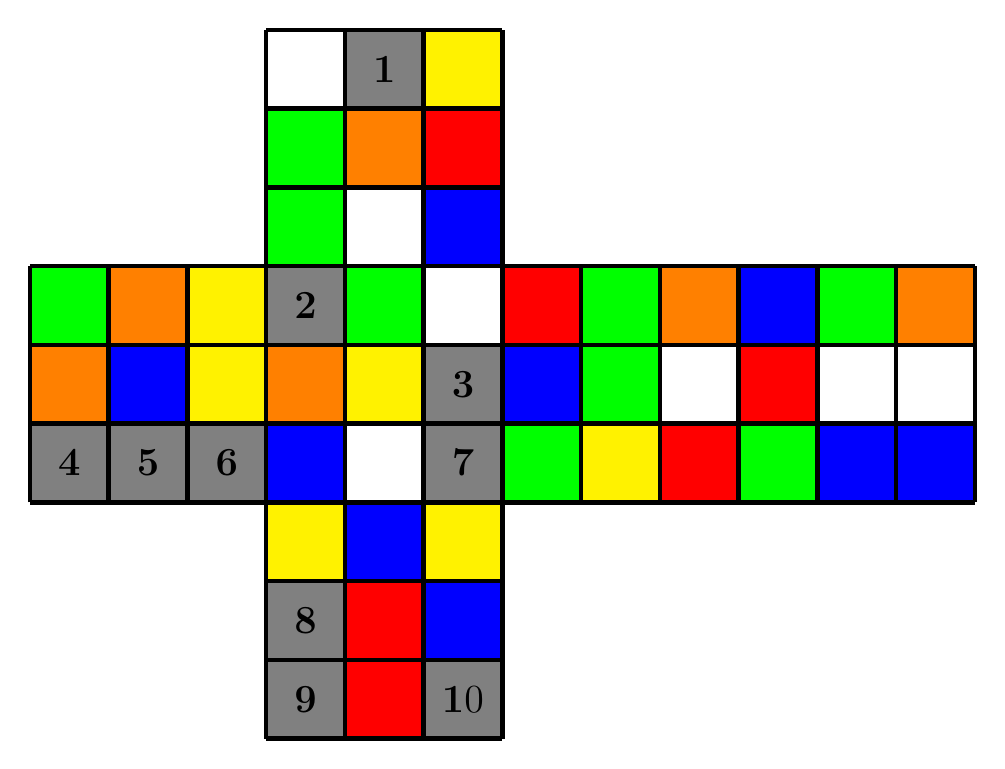
\begin{tikzpicture}[every node/.style={minimum size=1cm-\pgflinewidth, outer sep=0pt}]
\node[fill=white] at (0.5,5.5) {};
\node[fill=gray] at (1.5,5.5) {\Large \textbf 1};
\node[fill=yellow] at (2.5,5.5) {};
\node[fill=green] at (0.5,4.5) {};
\node[fill=orange] at (1.5,4.5) {};
\node[fill=red] at (2.5,4.5) {};
\node[fill=green] at (0.5,3.5) {};
\node[fill=white] at (1.5,3.5) {};
\node[fill=blue] at (2.5,3.5) {};

\node[fill=green] at (-2.5,2.5) {};
\node[fill=orange] at (-1.5,2.5) {};
\node[fill=yellow] at (-0.5,2.5) {};
\node[fill=gray] at (0.5,2.5) {\Large \textbf 2};
\node[fill=green] at (1.5,2.5) {};
\node[fill=white] at (2.5,2.5) {};
\node[fill=red] at (3.5,2.5) {};
\node[fill=green] at (4.5,2.5) {};
\node[fill=orange] at (5.5,2.5) {};
\node[fill=blue] at (6.5,2.5) {};
\node[fill=green] at (7.5,2.5) {};
\node[fill=orange] at (8.5,2.5) {};

\node[fill=orange] at (-2.5,1.5) {};
\node[fill=blue] at (-1.5,1.5) {};
\node[fill=yellow] at (-0.5,1.5) {};
\node[fill=orange] at (0.5,1.5) {};
\node[fill=yellow] at (1.5,1.5) {};
\node[fill=gray] at (2.5,1.5) {\Large \textbf 3};
\node[fill=blue] at (3.5,1.5) {};
\node[fill=green] at (4.5,1.5) {};
\node[fill=white] at (5.5,1.5) {};
\node[fill=red] at (6.5,1.5) {};
\node[fill=white] at (7.5,1.5) {};
\node[fill=white] at (8.5,1.5) {};

\node[fill=gray] at (-2.5,0.5) {\Large \textbf 4};
\node[fill=gray] at (-1.5,0.5) {\Large \textbf 5};
\node[fill=gray] at (-0.5,0.5) {\Large \textbf 6};
\node[fill=blue] at (0.5,0.5) {};
\node[fill=white] at (1.5,0.5) {};
\node[fill=gray] at (2.5,0.5) {\Large \textbf 7};
\node[fill=green] at (3.5,0.5) {};
\node[fill=yellow] at (4.5,0.5) {};
\node[fill=red] at (5.5,0.5) {};
\node[fill=green] at (6.5,0.5) {};
\node[fill=blue] at (7.5,0.5) {};
\node[fill=blue] at (8.5,0.5) {};

\node[fill=yellow] at (0.5,-0.5) {};
\node[fill=blue] at (1.5,-0.5) {};
\node[fill=yellow] at (2.5,-0.5) {};
\node[fill=gray] at (0.5,-1.5) {\Large \textbf 8};
\node[fill=red] at (1.5,-1.5) {};
\node[fill=blue] at (2.5,-1.5) {};
\node[fill=gray] at (0.5,-2.5) {\Large \textbf 9};
\node[fill=red] at (1.5,-2.5) {};
\node[fill=gray] at (2.5,-2.5) {\Large \textbf 10};

\draw[step=1cm,color=black, ultra thick] (-3,0) grid (9,3);
\draw[step=1cm,color=black, ultra thick] (0,-3) grid (3,0);
\draw[step=1cm,color=black, ultra thick] (0,3) grid (3,6);    
\end{tikzpicture}
\vspace{0.1cm}
\\
\noindent\normalsize \newtime  \textbf{Solution 31: B U' R2 F B2 D B U2 F2 L' D2 F2 B2 L U2 R2 F2 D2 L2 B' L2 Rw'}
\vspace{1cm}



{\noindent\Large \textbf{No. 32\qquad Difficulty:$\bigstar\bigstar$}}
\vspace{0.2cm}\\
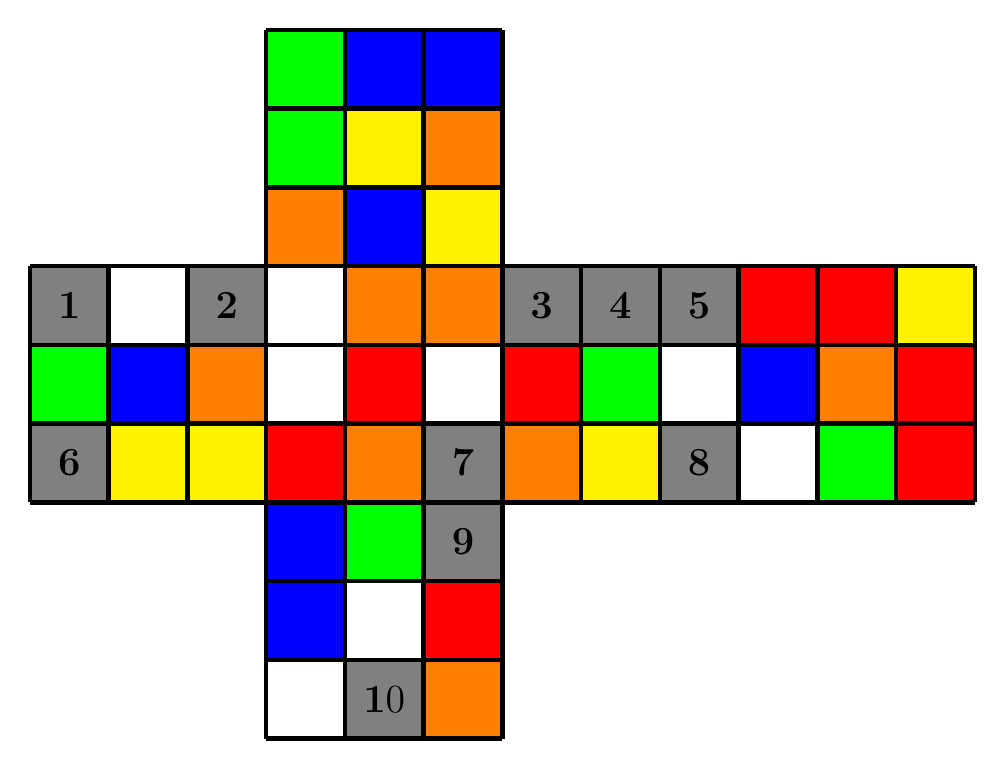
\begin{tikzpicture}[every node/.style={minimum size=1cm-\pgflinewidth, outer sep=0pt}]
\node[fill=green] at (0.5,5.5) {};
\node[fill=blue] at (1.5,5.5) {};
\node[fill=blue] at (2.5,5.5) {};
\node[fill=green] at (0.5,4.5) {};
\node[fill=yellow] at (1.5,4.5) {};
\node[fill=orange] at (2.5,4.5) {};
\node[fill=orange] at (0.5,3.5) {};
\node[fill=blue] at (1.5,3.5) {};
\node[fill=yellow] at (2.5,3.5) {};

\node[fill=gray] at (-2.5,2.5) {\Large \textbf 1};
\node[fill=white] at (-1.5,2.5) {};
\node[fill=gray] at (-0.5,2.5) {\Large \textbf 2};
\node[fill=white] at (0.5,2.5) {};
\node[fill=orange] at (1.5,2.5) {};
\node[fill=orange] at (2.5,2.5) {};
\node[fill=gray] at (3.5,2.5) {\Large \textbf 3};
\node[fill=gray] at (4.5,2.5) {\Large \textbf 4};
\node[fill=gray] at (5.5,2.5) {\Large \textbf 5};
\node[fill=red] at (6.5,2.5) {};
\node[fill=red] at (7.5,2.5) {};
\node[fill=yellow] at (8.5,2.5) {};

\node[fill=green] at (-2.5,1.5) {};
\node[fill=blue] at (-1.5,1.5) {};
\node[fill=orange] at (-0.5,1.5) {};
\node[fill=white] at (0.5,1.5) {};
\node[fill=red] at (1.5,1.5) {};
\node[fill=white] at (2.5,1.5) {};
\node[fill=red] at (3.5,1.5) {};
\node[fill=green] at (4.5,1.5) {};
\node[fill=white] at (5.5,1.5) {};
\node[fill=blue] at (6.5,1.5) {};
\node[fill=orange] at (7.5,1.5) {};
\node[fill=red] at (8.5,1.5) {};

\node[fill=gray] at (-2.5,0.5) {\Large \textbf 6};
\node[fill=yellow] at (-1.5,0.5) {};
\node[fill=yellow] at (-0.5,0.5) {};
\node[fill=red] at (0.5,0.5) {};
\node[fill=orange] at (1.5,0.5) {};
\node[fill=gray] at (2.5,0.5) {\Large \textbf 7};
\node[fill=orange] at (3.5,0.5) {};
\node[fill=yellow] at (4.5,0.5) {};
\node[fill=gray] at (5.5,0.5) {\Large \textbf 8};
\node[fill=white] at (6.5,0.5) {};
\node[fill=green] at (7.5,0.5) {};
\node[fill=red] at (8.5,0.5) {};

\node[fill=blue] at (0.5,-0.5) {};
\node[fill=green] at (1.5,-0.5) {};
\node[fill=gray] at (2.5,-0.5) {\Large \textbf 9};
\node[fill=blue] at (0.5,-1.5) {};
\node[fill=white] at (1.5,-1.5) {};
\node[fill=red] at (2.5,-1.5) {};
\node[fill=white] at (0.5,-2.5) {};
\node[fill=gray] at (1.5,-2.5) {\Large \textbf 10};
\node[fill=orange] at (2.5,-2.5) {};

\draw[step=1cm,color=black, ultra thick] (-3,0) grid (9,3);
\draw[step=1cm,color=black, ultra thick] (0,-3) grid (3,0);
\draw[step=1cm,color=black, ultra thick] (0,3) grid (3,6);    
\end{tikzpicture}
\vspace{0.1cm}
\\
\noindent\normalsize \newtime  \textbf{Solution 32: D' R F2 U' F2 R' F' U B R2 U2 R' F2 L' U2 L' U2 L' B2 R' U2}
\vspace{1cm}



{\noindent\Large \textbf{No. 33\qquad Difficulty:$\bigstar\bigstar$}}
\vspace{0.2cm}\\
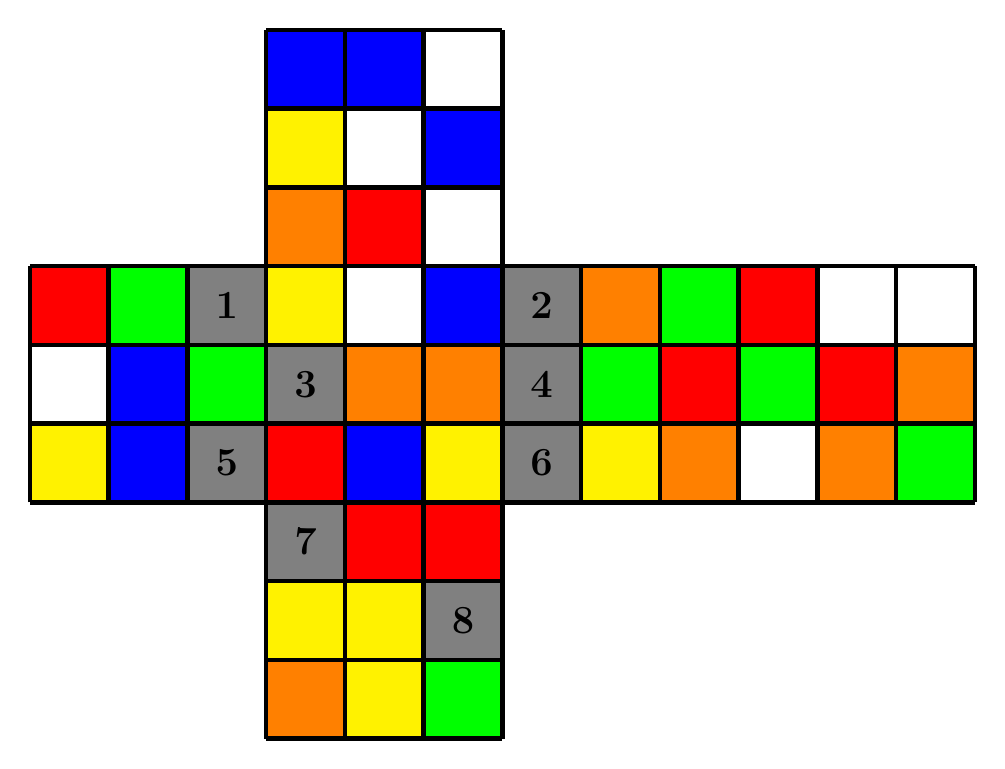
\begin{tikzpicture}[every node/.style={minimum size=1cm-\pgflinewidth, outer sep=0pt}]
\node[fill=blue] at (0.5,5.5) {};
\node[fill=blue] at (1.5,5.5) {};
\node[fill=white] at (2.5,5.5) {};
\node[fill=yellow] at (0.5,4.5) {};
\node[fill=white] at (1.5,4.5) {};
\node[fill=blue] at (2.5,4.5) {};
\node[fill=orange] at (0.5,3.5) {};
\node[fill=red] at (1.5,3.5) {};
\node[fill=white] at (2.5,3.5) {};

\node[fill=red] at (-2.5,2.5) {};
\node[fill=green] at (-1.5,2.5) {};
\node[fill=gray] at (-0.5,2.5) {\Large \textbf 1};
\node[fill=yellow] at (0.5,2.5) {};
\node[fill=white] at (1.5,2.5) {};
\node[fill=blue] at (2.5,2.5) {};
\node[fill=gray] at (3.5,2.5) {\Large \textbf 2};
\node[fill=orange] at (4.5,2.5) {};
\node[fill=green] at (5.5,2.5) {};
\node[fill=red] at (6.5,2.5) {};
\node[fill=white] at (7.5,2.5) {};
\node[fill=white] at (8.5,2.5) {};

\node[fill=white] at (-2.5,1.5) {};
\node[fill=blue] at (-1.5,1.5) {};
\node[fill=green] at (-0.5,1.5) {};
\node[fill=gray] at (0.5,1.5) {\Large \textbf 3};
\node[fill=orange] at (1.5,1.5) {};
\node[fill=orange] at (2.5,1.5) {};
\node[fill=gray] at (3.5,1.5) {\Large \textbf 4};
\node[fill=green] at (4.5,1.5) {};
\node[fill=red] at (5.5,1.5) {};
\node[fill=green] at (6.5,1.5) {};
\node[fill=red] at (7.5,1.5) {};
\node[fill=orange] at (8.5,1.5) {};

\node[fill=yellow] at (-2.5,0.5) {};
\node[fill=blue] at (-1.5,0.5) {};
\node[fill=gray] at (-0.5,0.5) {\Large \textbf 5};
\node[fill=red] at (0.5,0.5) {};
\node[fill=blue] at (1.5,0.5) {};
\node[fill=yellow] at (2.5,0.5) {};
\node[fill=gray] at (3.5,0.5) {\Large \textbf 6};
\node[fill=yellow] at (4.5,0.5) {};
\node[fill=orange] at (5.5,0.5) {};
\node[fill=white] at (6.5,0.5) {};
\node[fill=orange] at (7.5,0.5) {};
\node[fill=green] at (8.5,0.5) {};

\node[fill=gray] at (0.5,-0.5) {\Large \textbf 7};
\node[fill=red] at (1.5,-0.5) {};
\node[fill=red] at (2.5,-0.5) {};
\node[fill=yellow] at (0.5,-1.5) {};
\node[fill=yellow] at (1.5,-1.5) {};
\node[fill=gray] at (2.5,-1.5) {\Large \textbf 8};
\node[fill=orange] at (0.5,-2.5) {};
\node[fill=yellow] at (1.5,-2.5) {};
\node[fill=green] at (2.5,-2.5) {};

\draw[step=1cm,color=black, ultra thick] (-3,0) grid (9,3);
\draw[step=1cm,color=black, ultra thick] (0,-3) grid (3,0);
\draw[step=1cm,color=black, ultra thick] (0,3) grid (3,6);    
\end{tikzpicture}
\vspace{0.1cm}
\\
\noindent\normalsize \newtime  \textbf{Solution 33: R' D' F' L' D L' F U2 B2 R U2 B2 R2 L' U2 L2 D2 L' F2 B R2 Rw2}
\vspace{1cm}



{\noindent\Large \textbf{No. 34\qquad Difficulty:$\bigstar\bigstar$}}
\vspace{0.2cm}\\
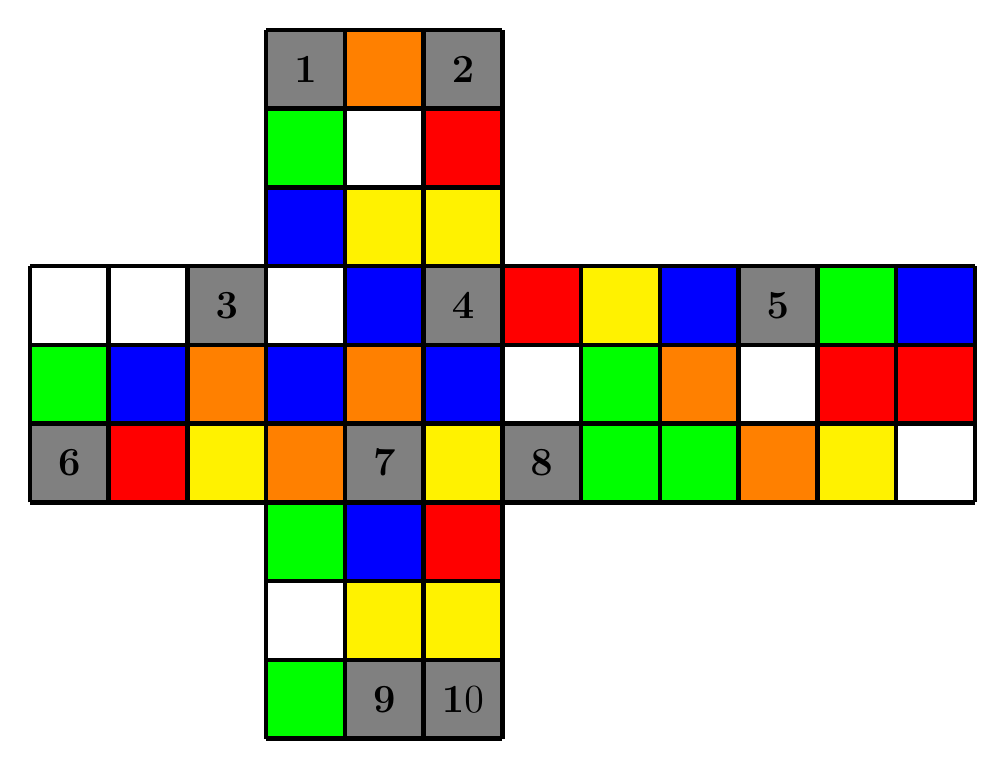
\begin{tikzpicture}[every node/.style={minimum size=1cm-\pgflinewidth, outer sep=0pt}]
\node[fill=gray] at (0.5,5.5) {\Large \textbf 1};
\node[fill=orange] at (1.5,5.5) {};
\node[fill=gray] at (2.5,5.5) {\Large \textbf 2};
\node[fill=green] at (0.5,4.5) {};
\node[fill=white] at (1.5,4.5) {};
\node[fill=red] at (2.5,4.5) {};
\node[fill=blue] at (0.5,3.5) {};
\node[fill=yellow] at (1.5,3.5) {};
\node[fill=yellow] at (2.5,3.5) {};

\node[fill=white] at (-2.5,2.5) {};
\node[fill=white] at (-1.5,2.5) {};
\node[fill=gray] at (-0.5,2.5) {\Large \textbf 3};
\node[fill=white] at (0.5,2.5) {};
\node[fill=blue] at (1.5,2.5) {};
\node[fill=gray] at (2.5,2.5) {\Large \textbf 4};
\node[fill=red] at (3.5,2.5) {};
\node[fill=yellow] at (4.5,2.5) {};
\node[fill=blue] at (5.5,2.5) {};
\node[fill=gray] at (6.5,2.5) {\Large \textbf 5};
\node[fill=green] at (7.5,2.5) {};
\node[fill=blue] at (8.5,2.5) {};

\node[fill=green] at (-2.5,1.5) {};
\node[fill=blue] at (-1.5,1.5) {};
\node[fill=orange] at (-0.5,1.5) {};
\node[fill=blue] at (0.5,1.5) {};
\node[fill=orange] at (1.5,1.5) {};
\node[fill=blue] at (2.5,1.5) {};
\node[fill=white] at (3.5,1.5) {};
\node[fill=green] at (4.5,1.5) {};
\node[fill=orange] at (5.5,1.5) {};
\node[fill=white] at (6.5,1.5) {};
\node[fill=red] at (7.5,1.5) {};
\node[fill=red] at (8.5,1.5) {};

\node[fill=gray] at (-2.5,0.5) {\Large \textbf 6};
\node[fill=red] at (-1.5,0.5) {};
\node[fill=yellow] at (-0.5,0.5) {};
\node[fill=orange] at (0.5,0.5) {};
\node[fill=gray] at (1.5,0.5) {\Large \textbf 7};
\node[fill=yellow] at (2.5,0.5) {};
\node[fill=gray] at (3.5,0.5) {\Large \textbf 8};
\node[fill=green] at (4.5,0.5) {};
\node[fill=green] at (5.5,0.5) {};
\node[fill=orange] at (6.5,0.5) {};
\node[fill=yellow] at (7.5,0.5) {};
\node[fill=white] at (8.5,0.5) {};

\node[fill=green] at (0.5,-0.5) {};
\node[fill=blue] at (1.5,-0.5) {};
\node[fill=red] at (2.5,-0.5) {};
\node[fill=white] at (0.5,-1.5) {};
\node[fill=yellow] at (1.5,-1.5) {};
\node[fill=yellow] at (2.5,-1.5) {};
\node[fill=green] at (0.5,-2.5) {};
\node[fill=gray] at (1.5,-2.5) {\Large \textbf 9};
\node[fill=gray] at (2.5,-2.5) {\Large \textbf 10};

\draw[step=1cm,color=black, ultra thick] (-3,0) grid (9,3);
\draw[step=1cm,color=black, ultra thick] (0,-3) grid (3,0);
\draw[step=1cm,color=black, ultra thick] (0,3) grid (3,6);    
\end{tikzpicture}
\vspace{0.1cm}
\\
\noindent\normalsize \newtime  \textbf{Solution 34: D B' R' F R2 F U2 R2 B D2 F L2 B F' U' F2 U2 R B' L D2 Rw2}
\vspace{1cm}



{\noindent\Large \textbf{No. 35\qquad Difficulty:$\bigstar\bigstar$}}
\vspace{0.2cm}\\
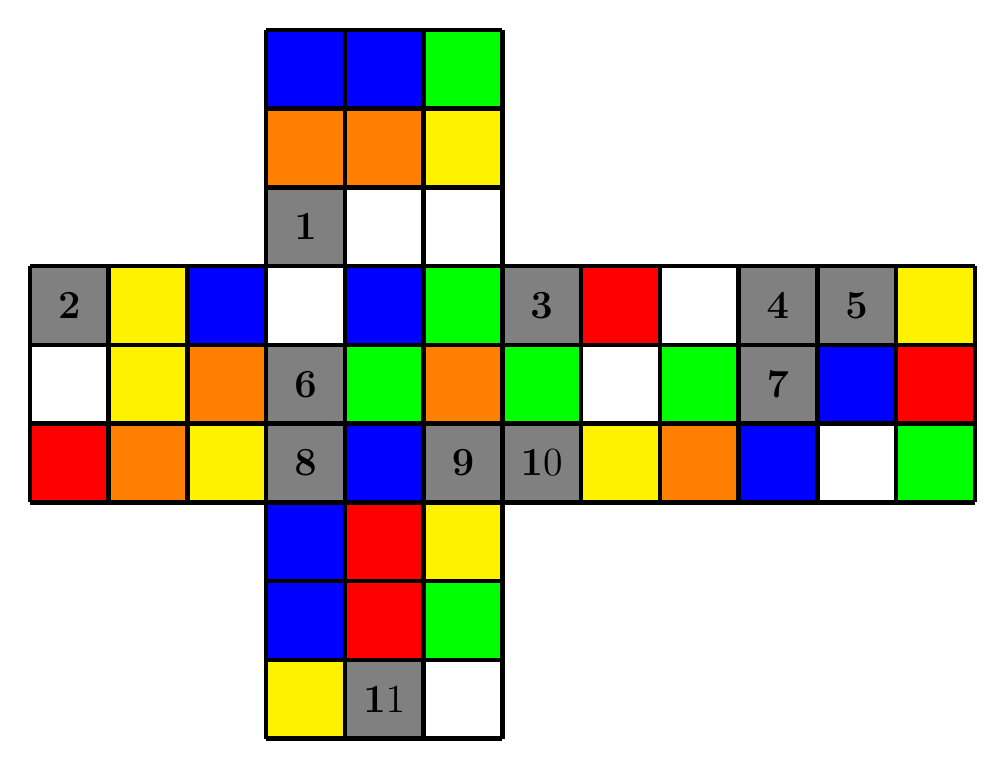
\begin{tikzpicture}[every node/.style={minimum size=1cm-\pgflinewidth, outer sep=0pt}]
\node[fill=blue] at (0.5,5.5) {};
\node[fill=blue] at (1.5,5.5) {};
\node[fill=green] at (2.5,5.5) {};
\node[fill=orange] at (0.5,4.5) {};
\node[fill=orange] at (1.5,4.5) {};
\node[fill=yellow] at (2.5,4.5) {};
\node[fill=gray] at (0.5,3.5) {\Large \textbf 1};
\node[fill=white] at (1.5,3.5) {};
\node[fill=white] at (2.5,3.5) {};

\node[fill=gray] at (-2.5,2.5) {\Large \textbf 2};
\node[fill=yellow] at (-1.5,2.5) {};
\node[fill=blue] at (-0.5,2.5) {};
\node[fill=white] at (0.5,2.5) {};
\node[fill=blue] at (1.5,2.5) {};
\node[fill=green] at (2.5,2.5) {};
\node[fill=gray] at (3.5,2.5) {\Large \textbf 3};
\node[fill=red] at (4.5,2.5) {};
\node[fill=white] at (5.5,2.5) {};
\node[fill=gray] at (6.5,2.5) {\Large \textbf 4};
\node[fill=gray] at (7.5,2.5) {\Large \textbf 5};
\node[fill=yellow] at (8.5,2.5) {};

\node[fill=white] at (-2.5,1.5) {};
\node[fill=yellow] at (-1.5,1.5) {};
\node[fill=orange] at (-0.5,1.5) {};
\node[fill=gray] at (0.5,1.5) {\Large \textbf 6};
\node[fill=green] at (1.5,1.5) {};
\node[fill=orange] at (2.5,1.5) {};
\node[fill=green] at (3.5,1.5) {};
\node[fill=white] at (4.5,1.5) {};
\node[fill=green] at (5.5,1.5) {};
\node[fill=gray] at (6.5,1.5) {\Large \textbf 7};
\node[fill=blue] at (7.5,1.5) {};
\node[fill=red] at (8.5,1.5) {};

\node[fill=red] at (-2.5,0.5) {};
\node[fill=orange] at (-1.5,0.5) {};
\node[fill=yellow] at (-0.5,0.5) {};
\node[fill=gray] at (0.5,0.5) {\Large \textbf 8};
\node[fill=blue] at (1.5,0.5) {};
\node[fill=gray] at (2.5,0.5) {\Large \textbf 9};
\node[fill=gray] at (3.5,0.5) {\Large \textbf 10};
\node[fill=yellow] at (4.5,0.5) {};
\node[fill=orange] at (5.5,0.5) {};
\node[fill=blue] at (6.5,0.5) {};
\node[fill=white] at (7.5,0.5) {};
\node[fill=green] at (8.5,0.5) {};

\node[fill=blue] at (0.5,-0.5) {};
\node[fill=red] at (1.5,-0.5) {};
\node[fill=yellow] at (2.5,-0.5) {};
\node[fill=blue] at (0.5,-1.5) {};
\node[fill=red] at (1.5,-1.5) {};
\node[fill=green] at (2.5,-1.5) {};
\node[fill=yellow] at (0.5,-2.5) {};
\node[fill=gray] at (1.5,-2.5) {\Large \textbf 11};
\node[fill=white] at (2.5,-2.5) {};

\draw[step=1cm,color=black, ultra thick] (-3,0) grid (9,3);
\draw[step=1cm,color=black, ultra thick] (0,-3) grid (3,0);
\draw[step=1cm,color=black, ultra thick] (0,3) grid (3,6);    
\end{tikzpicture}
\vspace{0.1cm}
\\
\noindent\normalsize \newtime  \textbf{Solution 35: F' L' F B D F' U' R' F' R2 F U2 L2 B R2 B2 L2 B' L2 F Rw' Uw}
\vspace{1cm}



{\noindent\Large \textbf{No. 36\qquad Difficulty:$\bigstar\bigstar$}}
\vspace{0.2cm}\\
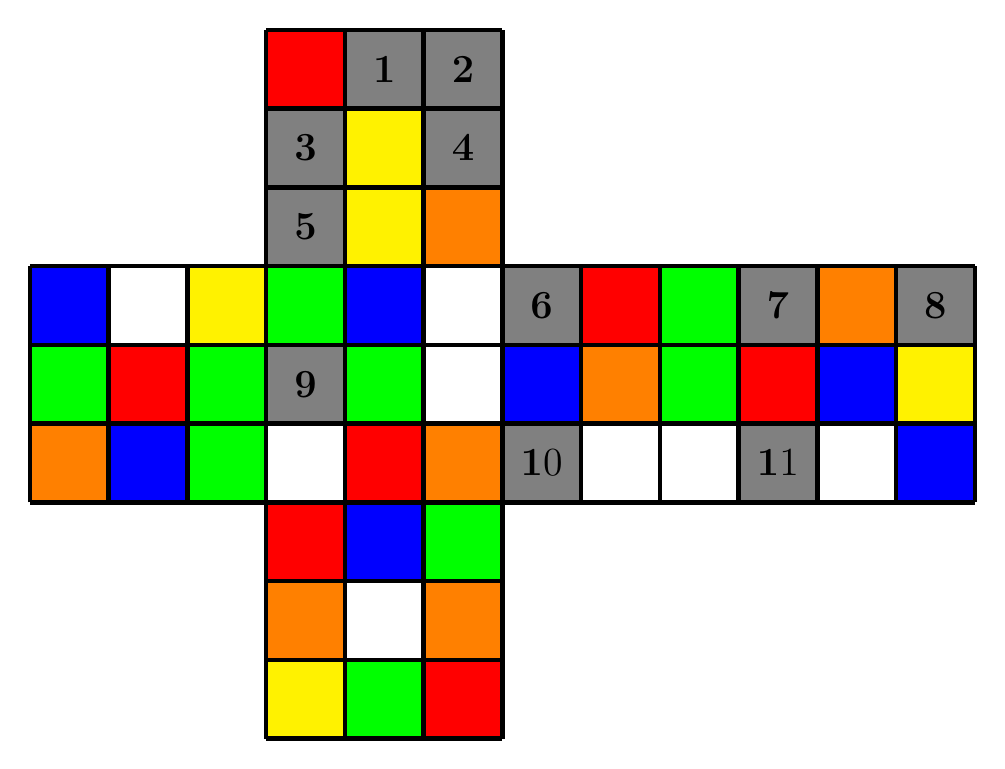
\begin{tikzpicture}[every node/.style={minimum size=1cm-\pgflinewidth, outer sep=0pt}]
\node[fill=red] at (0.5,5.5) {};
\node[fill=gray] at (1.5,5.5) {\Large \textbf 1};
\node[fill=gray] at (2.5,5.5) {\Large \textbf 2};
\node[fill=gray] at (0.5,4.5) {\Large \textbf 3};
\node[fill=yellow] at (1.5,4.5) {};
\node[fill=gray] at (2.5,4.5) {\Large \textbf 4};
\node[fill=gray] at (0.5,3.5) {\Large \textbf 5};
\node[fill=yellow] at (1.5,3.5) {};
\node[fill=orange] at (2.5,3.5) {};

\node[fill=blue] at (-2.5,2.5) {};
\node[fill=white] at (-1.5,2.5) {};
\node[fill=yellow] at (-0.5,2.5) {};
\node[fill=green] at (0.5,2.5) {};
\node[fill=blue] at (1.5,2.5) {};
\node[fill=white] at (2.5,2.5) {};
\node[fill=gray] at (3.5,2.5) {\Large \textbf 6};
\node[fill=red] at (4.5,2.5) {};
\node[fill=green] at (5.5,2.5) {};
\node[fill=gray] at (6.5,2.5) {\Large \textbf 7};
\node[fill=orange] at (7.5,2.5) {};
\node[fill=gray] at (8.5,2.5) {\Large \textbf 8};

\node[fill=green] at (-2.5,1.5) {};
\node[fill=red] at (-1.5,1.5) {};
\node[fill=green] at (-0.5,1.5) {};
\node[fill=gray] at (0.5,1.5) {\Large \textbf 9};
\node[fill=green] at (1.5,1.5) {};
\node[fill=white] at (2.5,1.5) {};
\node[fill=blue] at (3.5,1.5) {};
\node[fill=orange] at (4.5,1.5) {};
\node[fill=green] at (5.5,1.5) {};
\node[fill=red] at (6.5,1.5) {};
\node[fill=blue] at (7.5,1.5) {};
\node[fill=yellow] at (8.5,1.5) {};

\node[fill=orange] at (-2.5,0.5) {};
\node[fill=blue] at (-1.5,0.5) {};
\node[fill=green] at (-0.5,0.5) {};
\node[fill=white] at (0.5,0.5) {};
\node[fill=red] at (1.5,0.5) {};
\node[fill=orange] at (2.5,0.5) {};
\node[fill=gray] at (3.5,0.5) {\Large \textbf 10};
\node[fill=white] at (4.5,0.5) {};
\node[fill=white] at (5.5,0.5) {};
\node[fill=gray] at (6.5,0.5) {\Large \textbf 11};
\node[fill=white] at (7.5,0.5) {};
\node[fill=blue] at (8.5,0.5) {};

\node[fill=red] at (0.5,-0.5) {};
\node[fill=blue] at (1.5,-0.5) {};
\node[fill=green] at (2.5,-0.5) {};
\node[fill=orange] at (0.5,-1.5) {};
\node[fill=white] at (1.5,-1.5) {};
\node[fill=orange] at (2.5,-1.5) {};
\node[fill=yellow] at (0.5,-2.5) {};
\node[fill=green] at (1.5,-2.5) {};
\node[fill=red] at (2.5,-2.5) {};

\draw[step=1cm,color=black, ultra thick] (-3,0) grid (9,3);
\draw[step=1cm,color=black, ultra thick] (0,-3) grid (3,0);
\draw[step=1cm,color=black, ultra thick] (0,3) grid (3,6);    
\end{tikzpicture}
\vspace{0.1cm}
\\
\noindent\normalsize \newtime  \textbf{Solution 36: R' F2 U2 F2 D2 L2 D F2 U2 L2 B2 U' L2 R' D' L2 B' D' B2 U F' Uw}
\vspace{1cm}



{\noindent\Large \textbf{No. 37\qquad Difficulty:$\bigstar\bigstar$}}
\vspace{0.2cm}\\
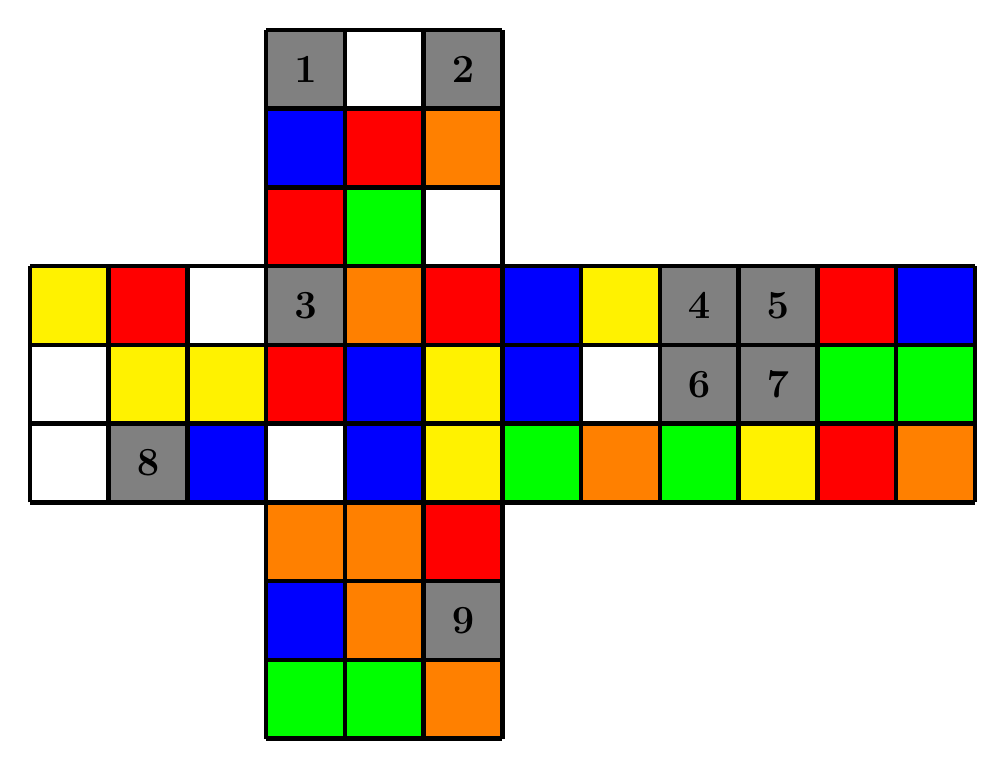
\begin{tikzpicture}[every node/.style={minimum size=1cm-\pgflinewidth, outer sep=0pt}]
\node[fill=gray] at (0.5,5.5) {\Large \textbf 1};
\node[fill=white] at (1.5,5.5) {};
\node[fill=gray] at (2.5,5.5) {\Large \textbf 2};
\node[fill=blue] at (0.5,4.5) {};
\node[fill=red] at (1.5,4.5) {};
\node[fill=orange] at (2.5,4.5) {};
\node[fill=red] at (0.5,3.5) {};
\node[fill=green] at (1.5,3.5) {};
\node[fill=white] at (2.5,3.5) {};

\node[fill=yellow] at (-2.5,2.5) {};
\node[fill=red] at (-1.5,2.5) {};
\node[fill=white] at (-0.5,2.5) {};
\node[fill=gray] at (0.5,2.5) {\Large \textbf 3};
\node[fill=orange] at (1.5,2.5) {};
\node[fill=red] at (2.5,2.5) {};
\node[fill=blue] at (3.5,2.5) {};
\node[fill=yellow] at (4.5,2.5) {};
\node[fill=gray] at (5.5,2.5) {\Large \textbf 4};
\node[fill=gray] at (6.5,2.5) {\Large \textbf 5};
\node[fill=red] at (7.5,2.5) {};
\node[fill=blue] at (8.5,2.5) {};

\node[fill=white] at (-2.5,1.5) {};
\node[fill=yellow] at (-1.5,1.5) {};
\node[fill=yellow] at (-0.5,1.5) {};
\node[fill=red] at (0.5,1.5) {};
\node[fill=blue] at (1.5,1.5) {};
\node[fill=yellow] at (2.5,1.5) {};
\node[fill=blue] at (3.5,1.5) {};
\node[fill=white] at (4.5,1.5) {};
\node[fill=gray] at (5.5,1.5) {\Large \textbf 6};
\node[fill=gray] at (6.5,1.5) {\Large \textbf 7};
\node[fill=green] at (7.5,1.5) {};
\node[fill=green] at (8.5,1.5) {};

\node[fill=white] at (-2.5,0.5) {};
\node[fill=gray] at (-1.5,0.5) {\Large \textbf 8};
\node[fill=blue] at (-0.5,0.5) {};
\node[fill=white] at (0.5,0.5) {};
\node[fill=blue] at (1.5,0.5) {};
\node[fill=yellow] at (2.5,0.5) {};
\node[fill=green] at (3.5,0.5) {};
\node[fill=orange] at (4.5,0.5) {};
\node[fill=green] at (5.5,0.5) {};
\node[fill=yellow] at (6.5,0.5) {};
\node[fill=red] at (7.5,0.5) {};
\node[fill=orange] at (8.5,0.5) {};

\node[fill=orange] at (0.5,-0.5) {};
\node[fill=orange] at (1.5,-0.5) {};
\node[fill=red] at (2.5,-0.5) {};
\node[fill=blue] at (0.5,-1.5) {};
\node[fill=orange] at (1.5,-1.5) {};
\node[fill=gray] at (2.5,-1.5) {\Large \textbf 9};
\node[fill=green] at (0.5,-2.5) {};
\node[fill=green] at (1.5,-2.5) {};
\node[fill=orange] at (2.5,-2.5) {};

\draw[step=1cm,color=black, ultra thick] (-3,0) grid (9,3);
\draw[step=1cm,color=black, ultra thick] (0,-3) grid (3,0);
\draw[step=1cm,color=black, ultra thick] (0,3) grid (3,6);    
\end{tikzpicture}
\vspace{0.1cm}
\\
\noindent\normalsize \newtime  \textbf{Solution 37: R2 U R B2 L U' B F2 U F2 U' R2 L2 F2 U R2 D2 R2 D' R U2 Rw Uw'}
\vspace{1cm}



{\noindent\Large \textbf{No. 38\qquad Difficulty:$\bigstar\bigstar$}}
\vspace{0.2cm}\\
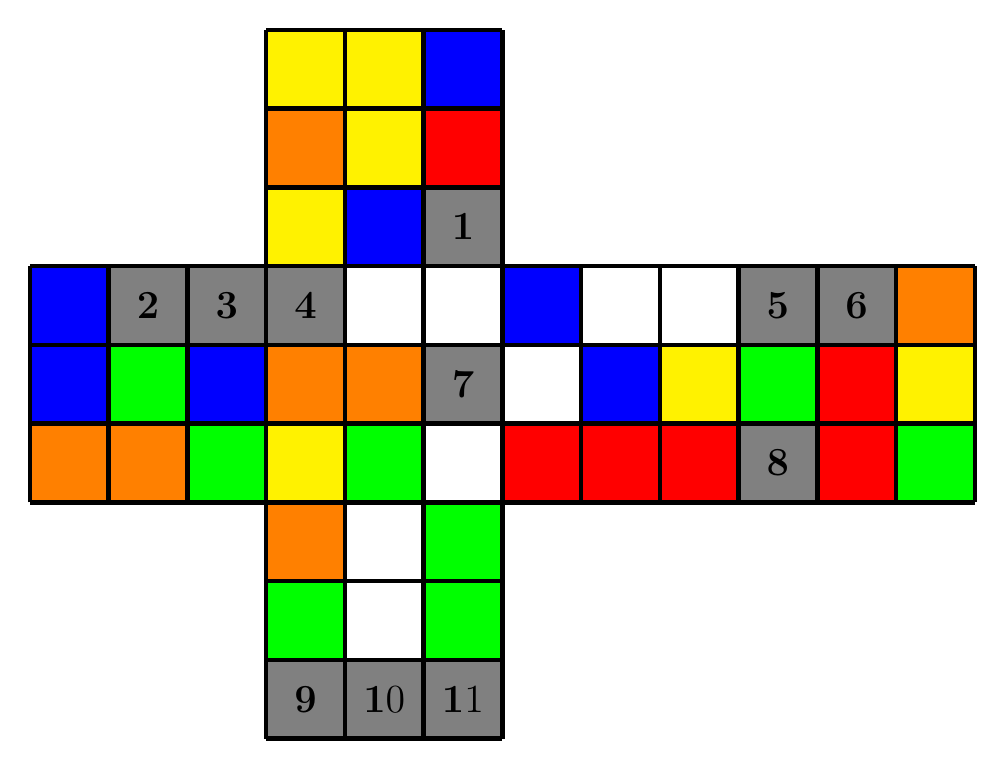
\begin{tikzpicture}[every node/.style={minimum size=1cm-\pgflinewidth, outer sep=0pt}]
\node[fill=yellow] at (0.5,5.5) {};
\node[fill=yellow] at (1.5,5.5) {};
\node[fill=blue] at (2.5,5.5) {};
\node[fill=orange] at (0.5,4.5) {};
\node[fill=yellow] at (1.5,4.5) {};
\node[fill=red] at (2.5,4.5) {};
\node[fill=yellow] at (0.5,3.5) {};
\node[fill=blue] at (1.5,3.5) {};
\node[fill=gray] at (2.5,3.5) {\Large \textbf 1};

\node[fill=blue] at (-2.5,2.5) {};
\node[fill=gray] at (-1.5,2.5) {\Large \textbf 2};
\node[fill=gray] at (-0.5,2.5) {\Large \textbf 3};
\node[fill=gray] at (0.5,2.5) {\Large \textbf 4};
\node[fill=white] at (1.5,2.5) {};
\node[fill=white] at (2.5,2.5) {};
\node[fill=blue] at (3.5,2.5) {};
\node[fill=white] at (4.5,2.5) {};
\node[fill=white] at (5.5,2.5) {};
\node[fill=gray] at (6.5,2.5) {\Large \textbf 5};
\node[fill=gray] at (7.5,2.5) {\Large \textbf 6};
\node[fill=orange] at (8.5,2.5) {};

\node[fill=blue] at (-2.5,1.5) {};
\node[fill=green] at (-1.5,1.5) {};
\node[fill=blue] at (-0.5,1.5) {};
\node[fill=orange] at (0.5,1.5) {};
\node[fill=orange] at (1.5,1.5) {};
\node[fill=gray] at (2.5,1.5) {\Large \textbf 7};
\node[fill=white] at (3.5,1.5) {};
\node[fill=blue] at (4.5,1.5) {};
\node[fill=yellow] at (5.5,1.5) {};
\node[fill=green] at (6.5,1.5) {};
\node[fill=red] at (7.5,1.5) {};
\node[fill=yellow] at (8.5,1.5) {};

\node[fill=orange] at (-2.5,0.5) {};
\node[fill=orange] at (-1.5,0.5) {};
\node[fill=green] at (-0.5,0.5) {};
\node[fill=yellow] at (0.5,0.5) {};
\node[fill=green] at (1.5,0.5) {};
\node[fill=white] at (2.5,0.5) {};
\node[fill=red] at (3.5,0.5) {};
\node[fill=red] at (4.5,0.5) {};
\node[fill=red] at (5.5,0.5) {};
\node[fill=gray] at (6.5,0.5) {\Large \textbf 8};
\node[fill=red] at (7.5,0.5) {};
\node[fill=green] at (8.5,0.5) {};

\node[fill=orange] at (0.5,-0.5) {};
\node[fill=white] at (1.5,-0.5) {};
\node[fill=green] at (2.5,-0.5) {};
\node[fill=green] at (0.5,-1.5) {};
\node[fill=white] at (1.5,-1.5) {};
\node[fill=green] at (2.5,-1.5) {};
\node[fill=gray] at (0.5,-2.5) {\Large \textbf 9};
\node[fill=gray] at (1.5,-2.5) {\Large \textbf 10};
\node[fill=gray] at (2.5,-2.5) {\Large \textbf 11};

\draw[step=1cm,color=black, ultra thick] (-3,0) grid (9,3);
\draw[step=1cm,color=black, ultra thick] (0,-3) grid (3,0);
\draw[step=1cm,color=black, ultra thick] (0,3) grid (3,6);    
\end{tikzpicture}
\vspace{0.1cm}
\\
\noindent\normalsize \newtime  \textbf{Solution 38: F D' B' U2 L2 F' D' L F L2 D2 F' U2 F2 U2 L2 D2 R' L2 Uw2}
\vspace{1cm}



{\noindent\Large \textbf{No. 39\qquad Difficulty:$\bigstar\bigstar$}}
\vspace{0.2cm}\\
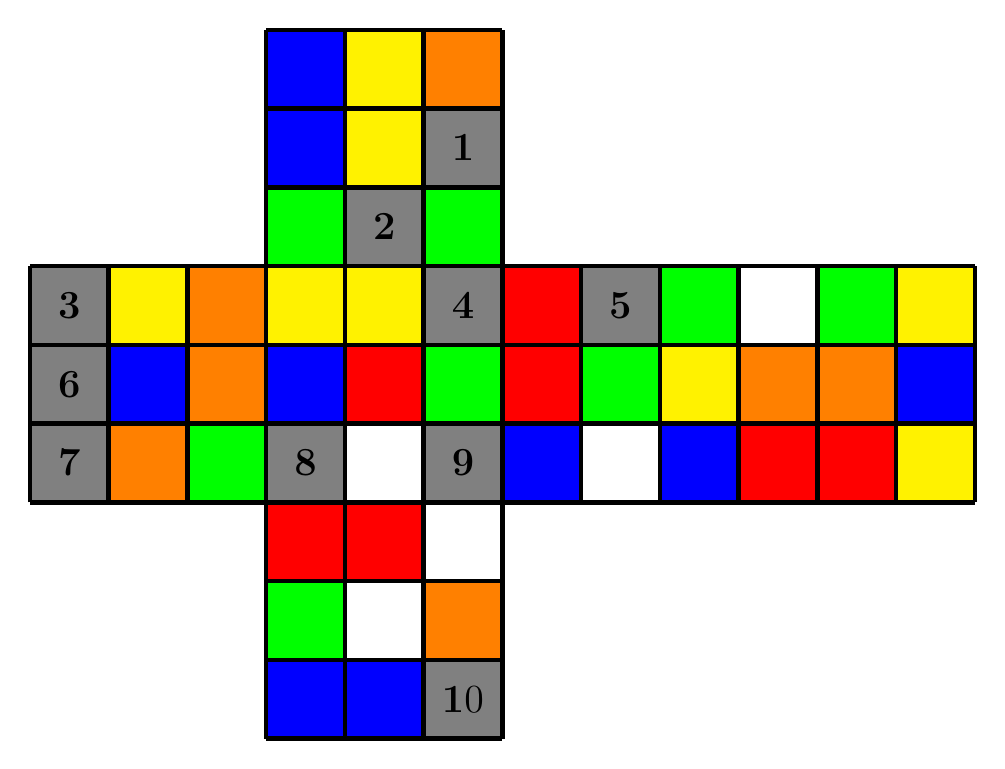
\begin{tikzpicture}[every node/.style={minimum size=1cm-\pgflinewidth, outer sep=0pt}]
\node[fill=blue] at (0.5,5.5) {};
\node[fill=yellow] at (1.5,5.5) {};
\node[fill=orange] at (2.5,5.5) {};
\node[fill=blue] at (0.5,4.5) {};
\node[fill=yellow] at (1.5,4.5) {};
\node[fill=gray] at (2.5,4.5) {\Large \textbf 1};
\node[fill=green] at (0.5,3.5) {};
\node[fill=gray] at (1.5,3.5) {\Large \textbf 2};
\node[fill=green] at (2.5,3.5) {};

\node[fill=gray] at (-2.5,2.5) {\Large \textbf 3};
\node[fill=yellow] at (-1.5,2.5) {};
\node[fill=orange] at (-0.5,2.5) {};
\node[fill=yellow] at (0.5,2.5) {};
\node[fill=yellow] at (1.5,2.5) {};
\node[fill=gray] at (2.5,2.5) {\Large \textbf 4};
\node[fill=red] at (3.5,2.5) {};
\node[fill=gray] at (4.5,2.5) {\Large \textbf 5};
\node[fill=green] at (5.5,2.5) {};
\node[fill=white] at (6.5,2.5) {};
\node[fill=green] at (7.5,2.5) {};
\node[fill=yellow] at (8.5,2.5) {};

\node[fill=gray] at (-2.5,1.5) {\Large \textbf 6};
\node[fill=blue] at (-1.5,1.5) {};
\node[fill=orange] at (-0.5,1.5) {};
\node[fill=blue] at (0.5,1.5) {};
\node[fill=red] at (1.5,1.5) {};
\node[fill=green] at (2.5,1.5) {};
\node[fill=red] at (3.5,1.5) {};
\node[fill=green] at (4.5,1.5) {};
\node[fill=yellow] at (5.5,1.5) {};
\node[fill=orange] at (6.5,1.5) {};
\node[fill=orange] at (7.5,1.5) {};
\node[fill=blue] at (8.5,1.5) {};

\node[fill=gray] at (-2.5,0.5) {\Large \textbf 7};
\node[fill=orange] at (-1.5,0.5) {};
\node[fill=green] at (-0.5,0.5) {};
\node[fill=gray] at (0.5,0.5) {\Large \textbf 8};
\node[fill=white] at (1.5,0.5) {};
\node[fill=gray] at (2.5,0.5) {\Large \textbf 9};
\node[fill=blue] at (3.5,0.5) {};
\node[fill=white] at (4.5,0.5) {};
\node[fill=blue] at (5.5,0.5) {};
\node[fill=red] at (6.5,0.5) {};
\node[fill=red] at (7.5,0.5) {};
\node[fill=yellow] at (8.5,0.5) {};

\node[fill=red] at (0.5,-0.5) {};
\node[fill=red] at (1.5,-0.5) {};
\node[fill=white] at (2.5,-0.5) {};
\node[fill=green] at (0.5,-1.5) {};
\node[fill=white] at (1.5,-1.5) {};
\node[fill=orange] at (2.5,-1.5) {};
\node[fill=blue] at (0.5,-2.5) {};
\node[fill=blue] at (1.5,-2.5) {};
\node[fill=gray] at (2.5,-2.5) {\Large \textbf 10};

\draw[step=1cm,color=black, ultra thick] (-3,0) grid (9,3);
\draw[step=1cm,color=black, ultra thick] (0,-3) grid (3,0);
\draw[step=1cm,color=black, ultra thick] (0,3) grid (3,6);    
\end{tikzpicture}
\vspace{0.1cm}
\\
\noindent\normalsize \newtime  \textbf{Solution 39: R F B2 L2 D L2 D2 R2 B2 F2 U' L2 U2 L' D' R' B' F' D' U' L2}
\vspace{1cm}



{\noindent\Large \textbf{No. 40\qquad Difficulty:$\bigstar\bigstar$}}
\vspace{0.2cm}\\
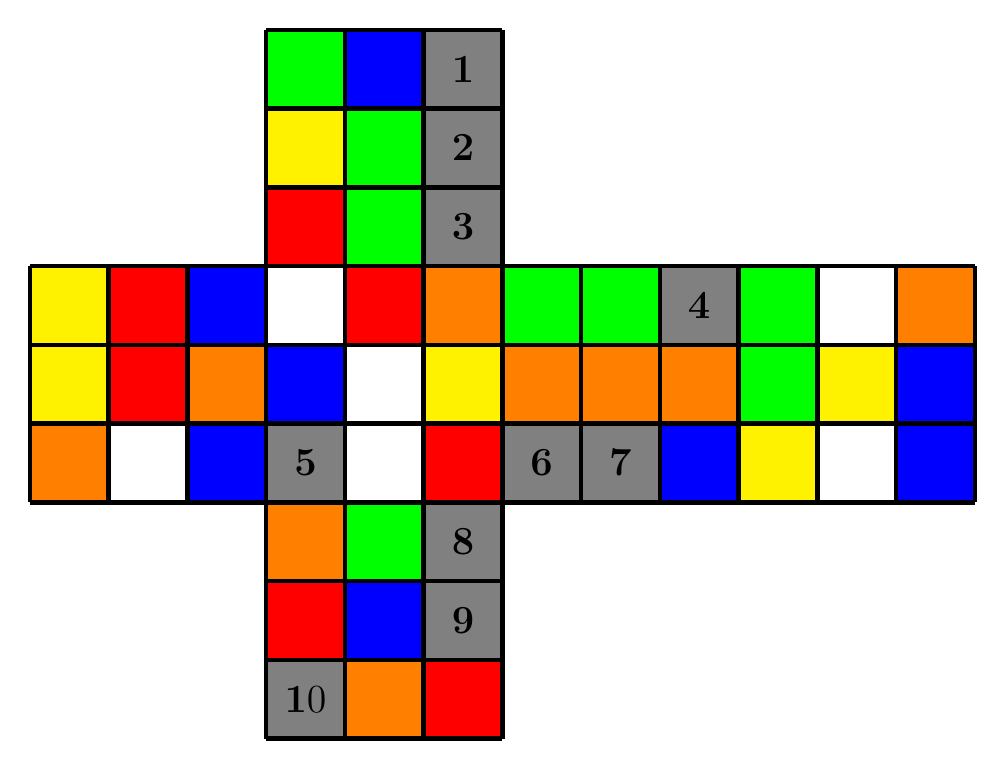
\begin{tikzpicture}[every node/.style={minimum size=1cm-\pgflinewidth, outer sep=0pt}]
\node[fill=green] at (0.5,5.5) {};
\node[fill=blue] at (1.5,5.5) {};
\node[fill=gray] at (2.5,5.5) {\Large \textbf 1};
\node[fill=yellow] at (0.5,4.5) {};
\node[fill=green] at (1.5,4.5) {};
\node[fill=gray] at (2.5,4.5) {\Large \textbf 2};
\node[fill=red] at (0.5,3.5) {};
\node[fill=green] at (1.5,3.5) {};
\node[fill=gray] at (2.5,3.5) {\Large \textbf 3};

\node[fill=yellow] at (-2.5,2.5) {};
\node[fill=red] at (-1.5,2.5) {};
\node[fill=blue] at (-0.5,2.5) {};
\node[fill=white] at (0.5,2.5) {};
\node[fill=red] at (1.5,2.5) {};
\node[fill=orange] at (2.5,2.5) {};
\node[fill=green] at (3.5,2.5) {};
\node[fill=green] at (4.5,2.5) {};
\node[fill=gray] at (5.5,2.5) {\Large \textbf 4};
\node[fill=green] at (6.5,2.5) {};
\node[fill=white] at (7.5,2.5) {};
\node[fill=orange] at (8.5,2.5) {};

\node[fill=yellow] at (-2.5,1.5) {};
\node[fill=red] at (-1.5,1.5) {};
\node[fill=orange] at (-0.5,1.5) {};
\node[fill=blue] at (0.5,1.5) {};
\node[fill=white] at (1.5,1.5) {};
\node[fill=yellow] at (2.5,1.5) {};
\node[fill=orange] at (3.5,1.5) {};
\node[fill=orange] at (4.5,1.5) {};
\node[fill=orange] at (5.5,1.5) {};
\node[fill=green] at (6.5,1.5) {};
\node[fill=yellow] at (7.5,1.5) {};
\node[fill=blue] at (8.5,1.5) {};

\node[fill=orange] at (-2.5,0.5) {};
\node[fill=white] at (-1.5,0.5) {};
\node[fill=blue] at (-0.5,0.5) {};
\node[fill=gray] at (0.5,0.5) {\Large \textbf 5};
\node[fill=white] at (1.5,0.5) {};
\node[fill=red] at (2.5,0.5) {};
\node[fill=gray] at (3.5,0.5) {\Large \textbf 6};
\node[fill=gray] at (4.5,0.5) {\Large \textbf 7};
\node[fill=blue] at (5.5,0.5) {};
\node[fill=yellow] at (6.5,0.5) {};
\node[fill=white] at (7.5,0.5) {};
\node[fill=blue] at (8.5,0.5) {};

\node[fill=orange] at (0.5,-0.5) {};
\node[fill=green] at (1.5,-0.5) {};
\node[fill=gray] at (2.5,-0.5) {\Large \textbf 8};
\node[fill=red] at (0.5,-1.5) {};
\node[fill=blue] at (1.5,-1.5) {};
\node[fill=gray] at (2.5,-1.5) {\Large \textbf 9};
\node[fill=gray] at (0.5,-2.5) {\Large \textbf 10};
\node[fill=orange] at (1.5,-2.5) {};
\node[fill=red] at (2.5,-2.5) {};

\draw[step=1cm,color=black, ultra thick] (-3,0) grid (9,3);
\draw[step=1cm,color=black, ultra thick] (0,-3) grid (3,0);
\draw[step=1cm,color=black, ultra thick] (0,3) grid (3,6);    
\end{tikzpicture}
\vspace{0.1cm}
\\
\noindent\normalsize \newtime  \textbf{Solution 40: L2 B' D2 B2 R2 D2 R' D2 F U' L2 U' F2 U B2 R2 U2 F2 U L2 D' Fw' Uw}
\vspace{1cm}



{\noindent\Large \textbf{No. 41\qquad Difficulty:$\bigstar\bigstar$}}
\vspace{0.2cm}\\
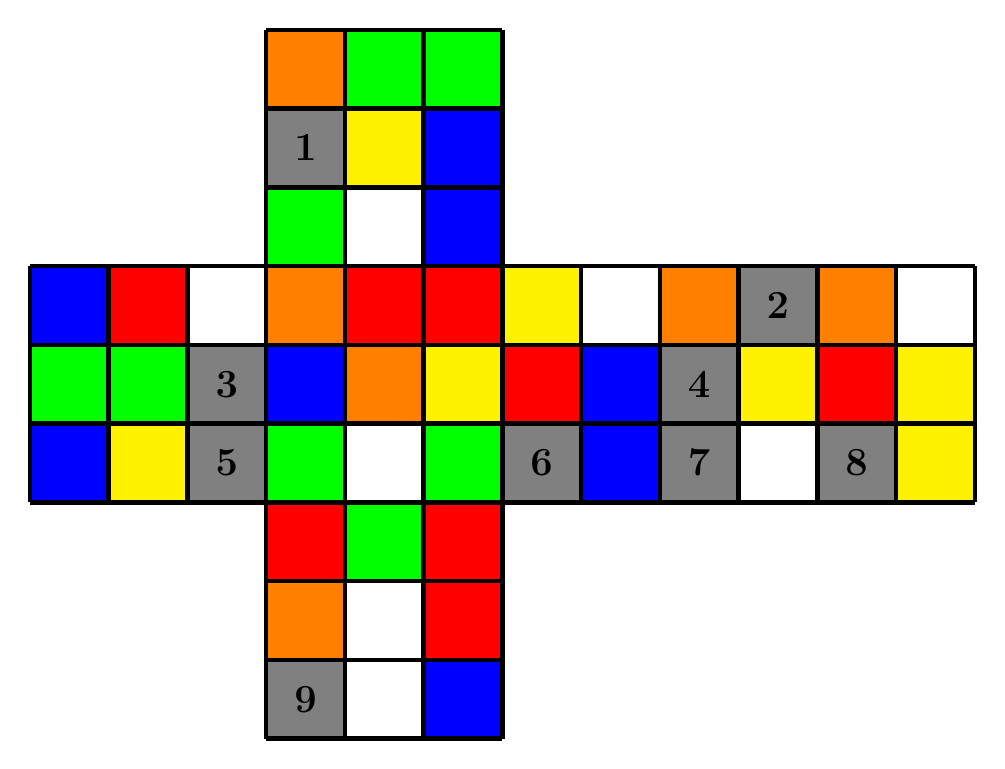
\begin{tikzpicture}[every node/.style={minimum size=1cm-\pgflinewidth, outer sep=0pt}]
\node[fill=orange] at (0.5,5.5) {};
\node[fill=green] at (1.5,5.5) {};
\node[fill=green] at (2.5,5.5) {};
\node[fill=gray] at (0.5,4.5) {\Large \textbf 1};
\node[fill=yellow] at (1.5,4.5) {};
\node[fill=blue] at (2.5,4.5) {};
\node[fill=green] at (0.5,3.5) {};
\node[fill=white] at (1.5,3.5) {};
\node[fill=blue] at (2.5,3.5) {};

\node[fill=blue] at (-2.5,2.5) {};
\node[fill=red] at (-1.5,2.5) {};
\node[fill=white] at (-0.5,2.5) {};
\node[fill=orange] at (0.5,2.5) {};
\node[fill=red] at (1.5,2.5) {};
\node[fill=red] at (2.5,2.5) {};
\node[fill=yellow] at (3.5,2.5) {};
\node[fill=white] at (4.5,2.5) {};
\node[fill=orange] at (5.5,2.5) {};
\node[fill=gray] at (6.5,2.5) {\Large \textbf 2};
\node[fill=orange] at (7.5,2.5) {};
\node[fill=white] at (8.5,2.5) {};

\node[fill=green] at (-2.5,1.5) {};
\node[fill=green] at (-1.5,1.5) {};
\node[fill=gray] at (-0.5,1.5) {\Large \textbf 3};
\node[fill=blue] at (0.5,1.5) {};
\node[fill=orange] at (1.5,1.5) {};
\node[fill=yellow] at (2.5,1.5) {};
\node[fill=red] at (3.5,1.5) {};
\node[fill=blue] at (4.5,1.5) {};
\node[fill=gray] at (5.5,1.5) {\Large \textbf 4};
\node[fill=yellow] at (6.5,1.5) {};
\node[fill=red] at (7.5,1.5) {};
\node[fill=yellow] at (8.5,1.5) {};

\node[fill=blue] at (-2.5,0.5) {};
\node[fill=yellow] at (-1.5,0.5) {};
\node[fill=gray] at (-0.5,0.5) {\Large \textbf 5};
\node[fill=green] at (0.5,0.5) {};
\node[fill=white] at (1.5,0.5) {};
\node[fill=green] at (2.5,0.5) {};
\node[fill=gray] at (3.5,0.5) {\Large \textbf 6};
\node[fill=blue] at (4.5,0.5) {};
\node[fill=gray] at (5.5,0.5) {\Large \textbf 7};
\node[fill=white] at (6.5,0.5) {};
\node[fill=gray] at (7.5,0.5) {\Large \textbf 8};
\node[fill=yellow] at (8.5,0.5) {};

\node[fill=red] at (0.5,-0.5) {};
\node[fill=green] at (1.5,-0.5) {};
\node[fill=red] at (2.5,-0.5) {};
\node[fill=orange] at (0.5,-1.5) {};
\node[fill=white] at (1.5,-1.5) {};
\node[fill=red] at (2.5,-1.5) {};
\node[fill=gray] at (0.5,-2.5) {\Large \textbf 9};
\node[fill=white] at (1.5,-2.5) {};
\node[fill=blue] at (2.5,-2.5) {};

\draw[step=1cm,color=black, ultra thick] (-3,0) grid (9,3);
\draw[step=1cm,color=black, ultra thick] (0,-3) grid (3,0);
\draw[step=1cm,color=black, ultra thick] (0,3) grid (3,6);    
\end{tikzpicture}
\vspace{0.1cm}
\\
\noindent\normalsize \newtime  \textbf{Solution 41: F2 U' F2 U' L2 B2 U2 B2 U R2 D' L2 B D' F L2 F R' U F L' Uw2}
\vspace{1cm}



{\noindent\Large \textbf{No. 42\qquad Difficulty:$\bigstar\bigstar$}}
\vspace{0.2cm}\\
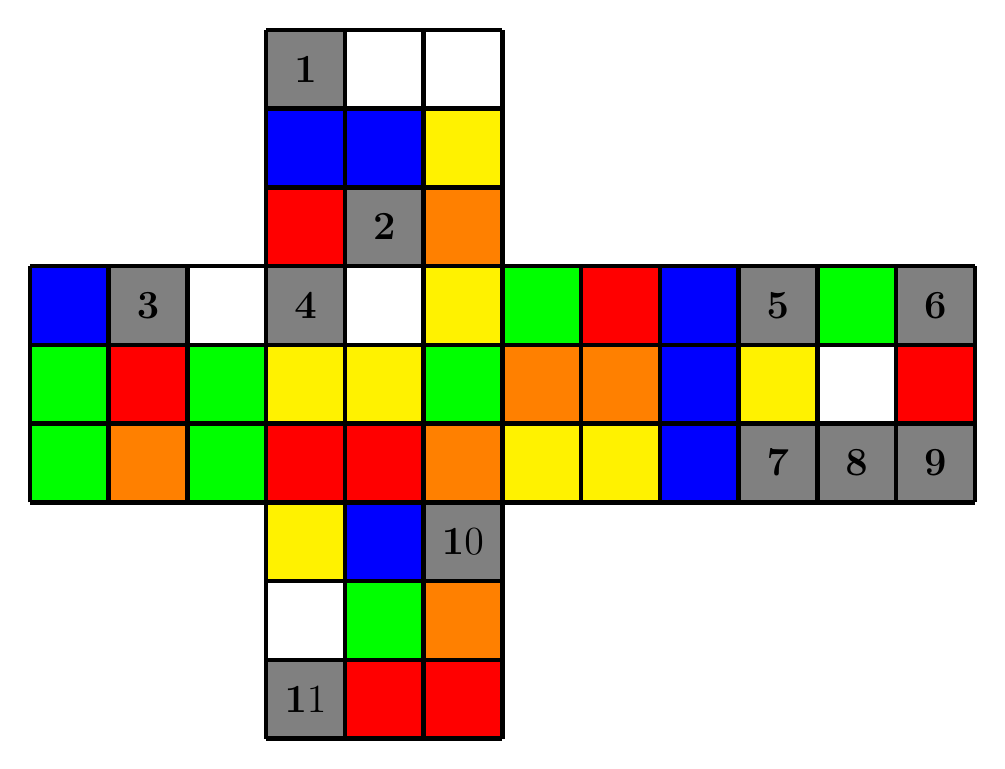
\begin{tikzpicture}[every node/.style={minimum size=1cm-\pgflinewidth, outer sep=0pt}]
\node[fill=gray] at (0.5,5.5) {\Large \textbf 1};
\node[fill=white] at (1.5,5.5) {};
\node[fill=white] at (2.5,5.5) {};
\node[fill=blue] at (0.5,4.5) {};
\node[fill=blue] at (1.5,4.5) {};
\node[fill=yellow] at (2.5,4.5) {};
\node[fill=red] at (0.5,3.5) {};
\node[fill=gray] at (1.5,3.5) {\Large \textbf 2};
\node[fill=orange] at (2.5,3.5) {};

\node[fill=blue] at (-2.5,2.5) {};
\node[fill=gray] at (-1.5,2.5) {\Large \textbf 3};
\node[fill=white] at (-0.5,2.5) {};
\node[fill=gray] at (0.5,2.5) {\Large \textbf 4};
\node[fill=white] at (1.5,2.5) {};
\node[fill=yellow] at (2.5,2.5) {};
\node[fill=green] at (3.5,2.5) {};
\node[fill=red] at (4.5,2.5) {};
\node[fill=blue] at (5.5,2.5) {};
\node[fill=gray] at (6.5,2.5) {\Large \textbf 5};
\node[fill=green] at (7.5,2.5) {};
\node[fill=gray] at (8.5,2.5) {\Large \textbf 6};

\node[fill=green] at (-2.5,1.5) {};
\node[fill=red] at (-1.5,1.5) {};
\node[fill=green] at (-0.5,1.5) {};
\node[fill=yellow] at (0.5,1.5) {};
\node[fill=yellow] at (1.5,1.5) {};
\node[fill=green] at (2.5,1.5) {};
\node[fill=orange] at (3.5,1.5) {};
\node[fill=orange] at (4.5,1.5) {};
\node[fill=blue] at (5.5,1.5) {};
\node[fill=yellow] at (6.5,1.5) {};
\node[fill=white] at (7.5,1.5) {};
\node[fill=red] at (8.5,1.5) {};

\node[fill=green] at (-2.5,0.5) {};
\node[fill=orange] at (-1.5,0.5) {};
\node[fill=green] at (-0.5,0.5) {};
\node[fill=red] at (0.5,0.5) {};
\node[fill=red] at (1.5,0.5) {};
\node[fill=orange] at (2.5,0.5) {};
\node[fill=yellow] at (3.5,0.5) {};
\node[fill=yellow] at (4.5,0.5) {};
\node[fill=blue] at (5.5,0.5) {};
\node[fill=gray] at (6.5,0.5) {\Large \textbf 7};
\node[fill=gray] at (7.5,0.5) {\Large \textbf 8};
\node[fill=gray] at (8.5,0.5) {\Large \textbf 9};

\node[fill=yellow] at (0.5,-0.5) {};
\node[fill=blue] at (1.5,-0.5) {};
\node[fill=gray] at (2.5,-0.5) {\Large \textbf 10};
\node[fill=white] at (0.5,-1.5) {};
\node[fill=green] at (1.5,-1.5) {};
\node[fill=orange] at (2.5,-1.5) {};
\node[fill=gray] at (0.5,-2.5) {\Large \textbf 11};
\node[fill=red] at (1.5,-2.5) {};
\node[fill=red] at (2.5,-2.5) {};

\draw[step=1cm,color=black, ultra thick] (-3,0) grid (9,3);
\draw[step=1cm,color=black, ultra thick] (0,-3) grid (3,0);
\draw[step=1cm,color=black, ultra thick] (0,3) grid (3,6);    
\end{tikzpicture}
\vspace{0.1cm}
\\
\noindent\normalsize \newtime  \textbf{Solution 42: D2 B2 L2 B2 D L2 R2 B2 D R2 D2 U' L F2 U' B' F2 U L' B R2 Fw Uw}
\vspace{1cm}



{\noindent\Large \textbf{No. 43\qquad Difficulty:$\bigstar\bigstar$}}
\vspace{0.2cm}\\
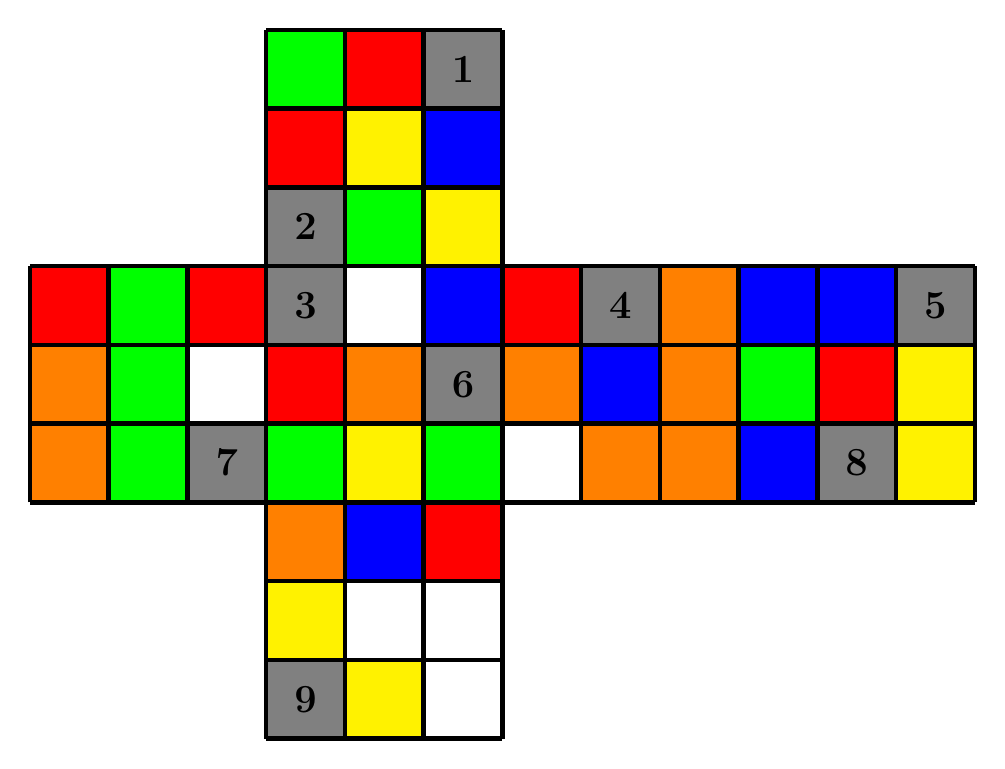
\begin{tikzpicture}[every node/.style={minimum size=1cm-\pgflinewidth, outer sep=0pt}]
\node[fill=green] at (0.5,5.5) {};
\node[fill=red] at (1.5,5.5) {};
\node[fill=gray] at (2.5,5.5) {\Large \textbf 1};
\node[fill=red] at (0.5,4.5) {};
\node[fill=yellow] at (1.5,4.5) {};
\node[fill=blue] at (2.5,4.5) {};
\node[fill=gray] at (0.5,3.5) {\Large \textbf 2};
\node[fill=green] at (1.5,3.5) {};
\node[fill=yellow] at (2.5,3.5) {};

\node[fill=red] at (-2.5,2.5) {};
\node[fill=green] at (-1.5,2.5) {};
\node[fill=red] at (-0.5,2.5) {};
\node[fill=gray] at (0.5,2.5) {\Large \textbf 3};
\node[fill=white] at (1.5,2.5) {};
\node[fill=blue] at (2.5,2.5) {};
\node[fill=red] at (3.5,2.5) {};
\node[fill=gray] at (4.5,2.5) {\Large \textbf 4};
\node[fill=orange] at (5.5,2.5) {};
\node[fill=blue] at (6.5,2.5) {};
\node[fill=blue] at (7.5,2.5) {};
\node[fill=gray] at (8.5,2.5) {\Large \textbf 5};

\node[fill=orange] at (-2.5,1.5) {};
\node[fill=green] at (-1.5,1.5) {};
\node[fill=white] at (-0.5,1.5) {};
\node[fill=red] at (0.5,1.5) {};
\node[fill=orange] at (1.5,1.5) {};
\node[fill=gray] at (2.5,1.5) {\Large \textbf 6};
\node[fill=orange] at (3.5,1.5) {};
\node[fill=blue] at (4.5,1.5) {};
\node[fill=orange] at (5.5,1.5) {};
\node[fill=green] at (6.5,1.5) {};
\node[fill=red] at (7.5,1.5) {};
\node[fill=yellow] at (8.5,1.5) {};

\node[fill=orange] at (-2.5,0.5) {};
\node[fill=green] at (-1.5,0.5) {};
\node[fill=gray] at (-0.5,0.5) {\Large \textbf 7};
\node[fill=green] at (0.5,0.5) {};
\node[fill=yellow] at (1.5,0.5) {};
\node[fill=green] at (2.5,0.5) {};
\node[fill=white] at (3.5,0.5) {};
\node[fill=orange] at (4.5,0.5) {};
\node[fill=orange] at (5.5,0.5) {};
\node[fill=blue] at (6.5,0.5) {};
\node[fill=gray] at (7.5,0.5) {\Large \textbf 8};
\node[fill=yellow] at (8.5,0.5) {};

\node[fill=orange] at (0.5,-0.5) {};
\node[fill=blue] at (1.5,-0.5) {};
\node[fill=red] at (2.5,-0.5) {};
\node[fill=yellow] at (0.5,-1.5) {};
\node[fill=white] at (1.5,-1.5) {};
\node[fill=white] at (2.5,-1.5) {};
\node[fill=gray] at (0.5,-2.5) {\Large \textbf 9};
\node[fill=yellow] at (1.5,-2.5) {};
\node[fill=white] at (2.5,-2.5) {};

\draw[step=1cm,color=black, ultra thick] (-3,0) grid (9,3);
\draw[step=1cm,color=black, ultra thick] (0,-3) grid (3,0);
\draw[step=1cm,color=black, ultra thick] (0,3) grid (3,6);    
\end{tikzpicture}
\vspace{0.1cm}
\\
\noindent\normalsize \newtime  \textbf{Solution 43: L U2 B2 U2 R B2 D2 L' D2 L' U2 D' F2 R' U L2 F' R2 U B' Uw2}
\vspace{1cm}



{\noindent\Large \textbf{No. 44\qquad Difficulty:$\bigstar\bigstar$}}
\vspace{0.2cm}\\
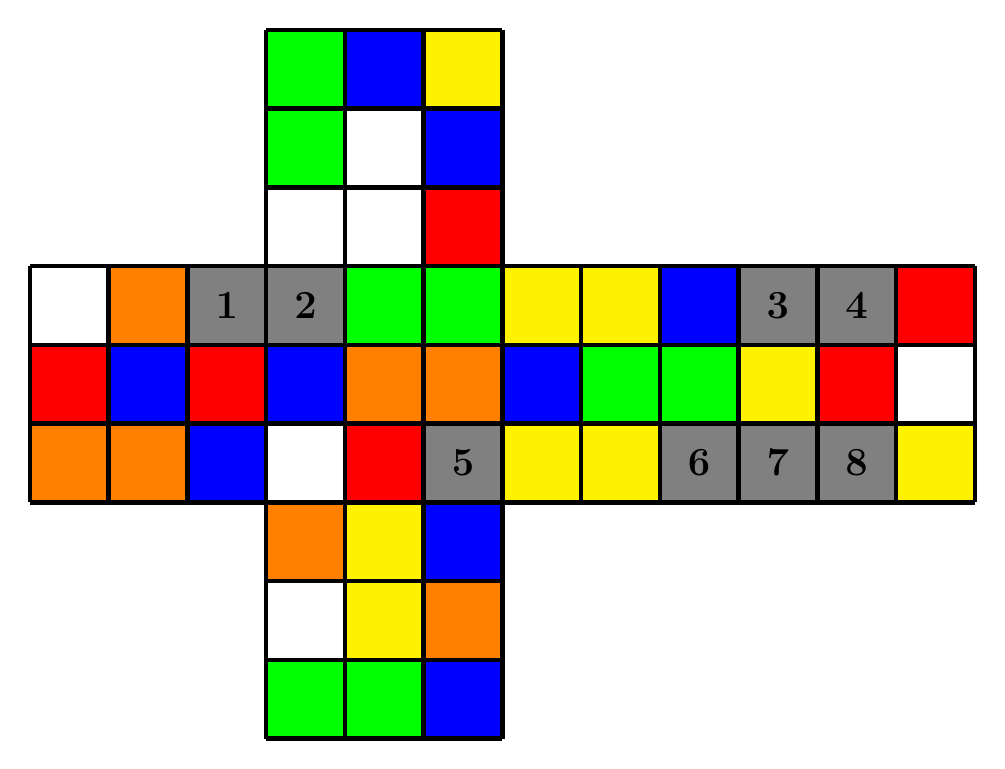
\begin{tikzpicture}[every node/.style={minimum size=1cm-\pgflinewidth, outer sep=0pt}]
\node[fill=green] at (0.5,5.5) {};
\node[fill=blue] at (1.5,5.5) {};
\node[fill=yellow] at (2.5,5.5) {};
\node[fill=green] at (0.5,4.5) {};
\node[fill=white] at (1.5,4.5) {};
\node[fill=blue] at (2.5,4.5) {};
\node[fill=white] at (0.5,3.5) {};
\node[fill=white] at (1.5,3.5) {};
\node[fill=red] at (2.5,3.5) {};

\node[fill=white] at (-2.5,2.5) {};
\node[fill=orange] at (-1.5,2.5) {};
\node[fill=gray] at (-0.5,2.5) {\Large \textbf 1};
\node[fill=gray] at (0.5,2.5) {\Large \textbf 2};
\node[fill=green] at (1.5,2.5) {};
\node[fill=green] at (2.5,2.5) {};
\node[fill=yellow] at (3.5,2.5) {};
\node[fill=yellow] at (4.5,2.5) {};
\node[fill=blue] at (5.5,2.5) {};
\node[fill=gray] at (6.5,2.5) {\Large \textbf 3};
\node[fill=gray] at (7.5,2.5) {\Large \textbf 4};
\node[fill=red] at (8.5,2.5) {};

\node[fill=red] at (-2.5,1.5) {};
\node[fill=blue] at (-1.5,1.5) {};
\node[fill=red] at (-0.5,1.5) {};
\node[fill=blue] at (0.5,1.5) {};
\node[fill=orange] at (1.5,1.5) {};
\node[fill=orange] at (2.5,1.5) {};
\node[fill=blue] at (3.5,1.5) {};
\node[fill=green] at (4.5,1.5) {};
\node[fill=green] at (5.5,1.5) {};
\node[fill=yellow] at (6.5,1.5) {};
\node[fill=red] at (7.5,1.5) {};
\node[fill=white] at (8.5,1.5) {};

\node[fill=orange] at (-2.5,0.5) {};
\node[fill=orange] at (-1.5,0.5) {};
\node[fill=blue] at (-0.5,0.5) {};
\node[fill=white] at (0.5,0.5) {};
\node[fill=red] at (1.5,0.5) {};
\node[fill=gray] at (2.5,0.5) {\Large \textbf 5};
\node[fill=yellow] at (3.5,0.5) {};
\node[fill=yellow] at (4.5,0.5) {};
\node[fill=gray] at (5.5,0.5) {\Large \textbf 6};
\node[fill=gray] at (6.5,0.5) {\Large \textbf 7};
\node[fill=gray] at (7.5,0.5) {\Large \textbf 8};
\node[fill=yellow] at (8.5,0.5) {};

\node[fill=orange] at (0.5,-0.5) {};
\node[fill=yellow] at (1.5,-0.5) {};
\node[fill=blue] at (2.5,-0.5) {};
\node[fill=white] at (0.5,-1.5) {};
\node[fill=yellow] at (1.5,-1.5) {};
\node[fill=orange] at (2.5,-1.5) {};
\node[fill=green] at (0.5,-2.5) {};
\node[fill=green] at (1.5,-2.5) {};
\node[fill=blue] at (2.5,-2.5) {};

\draw[step=1cm,color=black, ultra thick] (-3,0) grid (9,3);
\draw[step=1cm,color=black, ultra thick] (0,-3) grid (3,0);
\draw[step=1cm,color=black, ultra thick] (0,3) grid (3,6);    
\end{tikzpicture}
\vspace{0.1cm}
\\
\noindent\normalsize \newtime  \textbf{Solution 44: B' D2 L D F R2 L' B U2 B2 L2 D2 L U2 D2 L2 F2 U2 L' U2 D' Rw2}
\vspace{1cm}



{\noindent\Large \textbf{No. 45\qquad Difficulty:$\bigstar\bigstar$}}
\vspace{0.2cm}\\
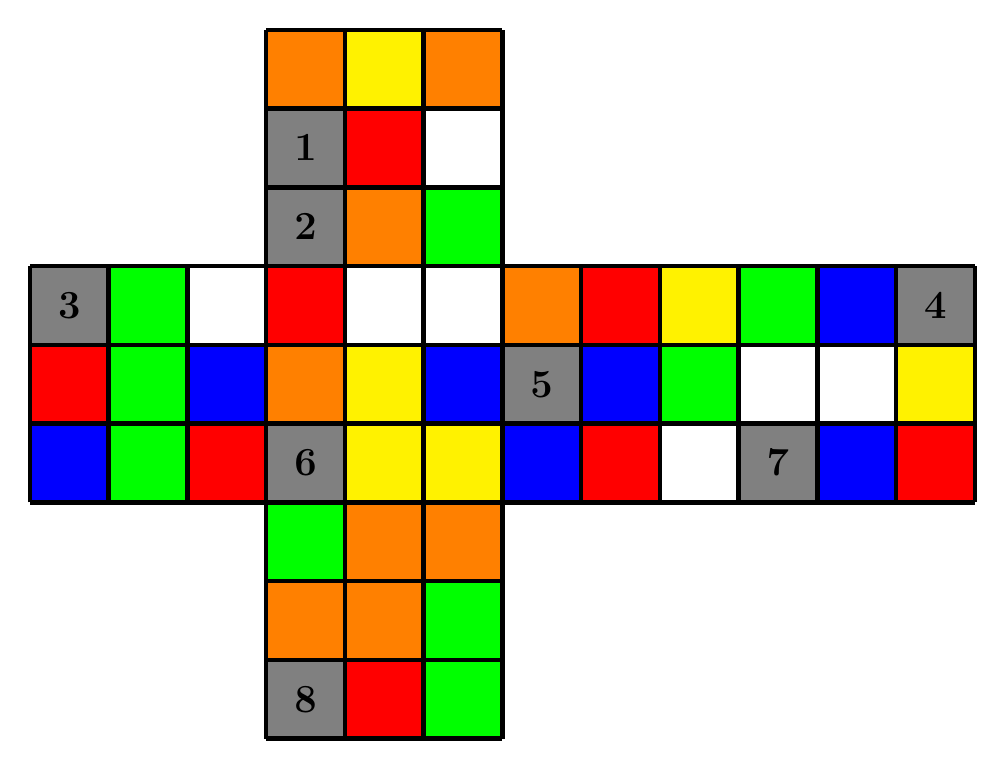
\begin{tikzpicture}[every node/.style={minimum size=1cm-\pgflinewidth, outer sep=0pt}]
\node[fill=orange] at (0.5,5.5) {};
\node[fill=yellow] at (1.5,5.5) {};
\node[fill=orange] at (2.5,5.5) {};
\node[fill=gray] at (0.5,4.5) {\Large \textbf 1};
\node[fill=red] at (1.5,4.5) {};
\node[fill=white] at (2.5,4.5) {};
\node[fill=gray] at (0.5,3.5) {\Large \textbf 2};
\node[fill=orange] at (1.5,3.5) {};
\node[fill=green] at (2.5,3.5) {};

\node[fill=gray] at (-2.5,2.5) {\Large \textbf 3};
\node[fill=green] at (-1.5,2.5) {};
\node[fill=white] at (-0.5,2.5) {};
\node[fill=red] at (0.5,2.5) {};
\node[fill=white] at (1.5,2.5) {};
\node[fill=white] at (2.5,2.5) {};
\node[fill=orange] at (3.5,2.5) {};
\node[fill=red] at (4.5,2.5) {};
\node[fill=yellow] at (5.5,2.5) {};
\node[fill=green] at (6.5,2.5) {};
\node[fill=blue] at (7.5,2.5) {};
\node[fill=gray] at (8.5,2.5) {\Large \textbf 4};

\node[fill=red] at (-2.5,1.5) {};
\node[fill=green] at (-1.5,1.5) {};
\node[fill=blue] at (-0.5,1.5) {};
\node[fill=orange] at (0.5,1.5) {};
\node[fill=yellow] at (1.5,1.5) {};
\node[fill=blue] at (2.5,1.5) {};
\node[fill=gray] at (3.5,1.5) {\Large \textbf 5};
\node[fill=blue] at (4.5,1.5) {};
\node[fill=green] at (5.5,1.5) {};
\node[fill=white] at (6.5,1.5) {};
\node[fill=white] at (7.5,1.5) {};
\node[fill=yellow] at (8.5,1.5) {};

\node[fill=blue] at (-2.5,0.5) {};
\node[fill=green] at (-1.5,0.5) {};
\node[fill=red] at (-0.5,0.5) {};
\node[fill=gray] at (0.5,0.5) {\Large \textbf 6};
\node[fill=yellow] at (1.5,0.5) {};
\node[fill=yellow] at (2.5,0.5) {};
\node[fill=blue] at (3.5,0.5) {};
\node[fill=red] at (4.5,0.5) {};
\node[fill=white] at (5.5,0.5) {};
\node[fill=gray] at (6.5,0.5) {\Large \textbf 7};
\node[fill=blue] at (7.5,0.5) {};
\node[fill=red] at (8.5,0.5) {};

\node[fill=green] at (0.5,-0.5) {};
\node[fill=orange] at (1.5,-0.5) {};
\node[fill=orange] at (2.5,-0.5) {};
\node[fill=orange] at (0.5,-1.5) {};
\node[fill=orange] at (1.5,-1.5) {};
\node[fill=green] at (2.5,-1.5) {};
\node[fill=gray] at (0.5,-2.5) {\Large \textbf 8};
\node[fill=red] at (1.5,-2.5) {};
\node[fill=green] at (2.5,-2.5) {};

\draw[step=1cm,color=black, ultra thick] (-3,0) grid (9,3);
\draw[step=1cm,color=black, ultra thick] (0,-3) grid (3,0);
\draw[step=1cm,color=black, ultra thick] (0,3) grid (3,6);    
\end{tikzpicture}
\vspace{0.1cm}
\\
\noindent\normalsize \newtime  \textbf{Solution 45: R' L2 D2 U L2 D' F2 D B2 U F2 U' L2 R' U' L2 R U L2 B' D2 Rw Uw2}
\vspace{1cm}



{\noindent\Large \textbf{No. 46\qquad Difficulty:$\bigstar\bigstar$}}
\vspace{0.2cm}\\
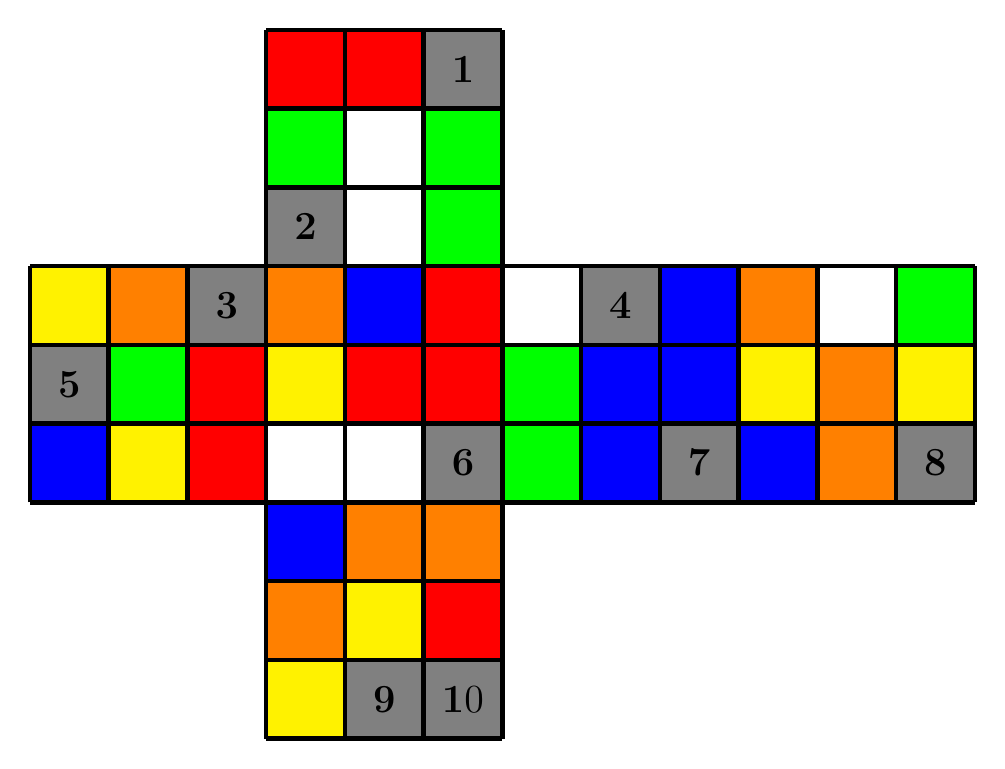
\begin{tikzpicture}[every node/.style={minimum size=1cm-\pgflinewidth, outer sep=0pt}]
\node[fill=red] at (0.5,5.5) {};
\node[fill=red] at (1.5,5.5) {};
\node[fill=gray] at (2.5,5.5) {\Large \textbf 1};
\node[fill=green] at (0.5,4.5) {};
\node[fill=white] at (1.5,4.5) {};
\node[fill=green] at (2.5,4.5) {};
\node[fill=gray] at (0.5,3.5) {\Large \textbf 2};
\node[fill=white] at (1.5,3.5) {};
\node[fill=green] at (2.5,3.5) {};

\node[fill=yellow] at (-2.5,2.5) {};
\node[fill=orange] at (-1.5,2.5) {};
\node[fill=gray] at (-0.5,2.5) {\Large \textbf 3};
\node[fill=orange] at (0.5,2.5) {};
\node[fill=blue] at (1.5,2.5) {};
\node[fill=red] at (2.5,2.5) {};
\node[fill=white] at (3.5,2.5) {};
\node[fill=gray] at (4.5,2.5) {\Large \textbf 4};
\node[fill=blue] at (5.5,2.5) {};
\node[fill=orange] at (6.5,2.5) {};
\node[fill=white] at (7.5,2.5) {};
\node[fill=green] at (8.5,2.5) {};

\node[fill=gray] at (-2.5,1.5) {\Large \textbf 5};
\node[fill=green] at (-1.5,1.5) {};
\node[fill=red] at (-0.5,1.5) {};
\node[fill=yellow] at (0.5,1.5) {};
\node[fill=red] at (1.5,1.5) {};
\node[fill=red] at (2.5,1.5) {};
\node[fill=green] at (3.5,1.5) {};
\node[fill=blue] at (4.5,1.5) {};
\node[fill=blue] at (5.5,1.5) {};
\node[fill=yellow] at (6.5,1.5) {};
\node[fill=orange] at (7.5,1.5) {};
\node[fill=yellow] at (8.5,1.5) {};

\node[fill=blue] at (-2.5,0.5) {};
\node[fill=yellow] at (-1.5,0.5) {};
\node[fill=red] at (-0.5,0.5) {};
\node[fill=white] at (0.5,0.5) {};
\node[fill=white] at (1.5,0.5) {};
\node[fill=gray] at (2.5,0.5) {\Large \textbf 6};
\node[fill=green] at (3.5,0.5) {};
\node[fill=blue] at (4.5,0.5) {};
\node[fill=gray] at (5.5,0.5) {\Large \textbf 7};
\node[fill=blue] at (6.5,0.5) {};
\node[fill=orange] at (7.5,0.5) {};
\node[fill=gray] at (8.5,0.5) {\Large \textbf 8};

\node[fill=blue] at (0.5,-0.5) {};
\node[fill=orange] at (1.5,-0.5) {};
\node[fill=orange] at (2.5,-0.5) {};
\node[fill=orange] at (0.5,-1.5) {};
\node[fill=yellow] at (1.5,-1.5) {};
\node[fill=red] at (2.5,-1.5) {};
\node[fill=yellow] at (0.5,-2.5) {};
\node[fill=gray] at (1.5,-2.5) {\Large \textbf 9};
\node[fill=gray] at (2.5,-2.5) {\Large \textbf 10};

\draw[step=1cm,color=black, ultra thick] (-3,0) grid (9,3);
\draw[step=1cm,color=black, ultra thick] (0,-3) grid (3,0);
\draw[step=1cm,color=black, ultra thick] (0,3) grid (3,6);    
\end{tikzpicture}
\vspace{0.1cm}
\\
\noindent\normalsize \newtime  \textbf{Solution 46: D2 L2 D2 U L2 U' L2 R2 B2 L2 R2 B L2 R D' B' L B' D' B2 F2 Rw2 Uw2}
\vspace{1cm}



{\noindent\Large \textbf{No. 47\qquad Difficulty:$\bigstar\bigstar$}}
\vspace{0.2cm}\\
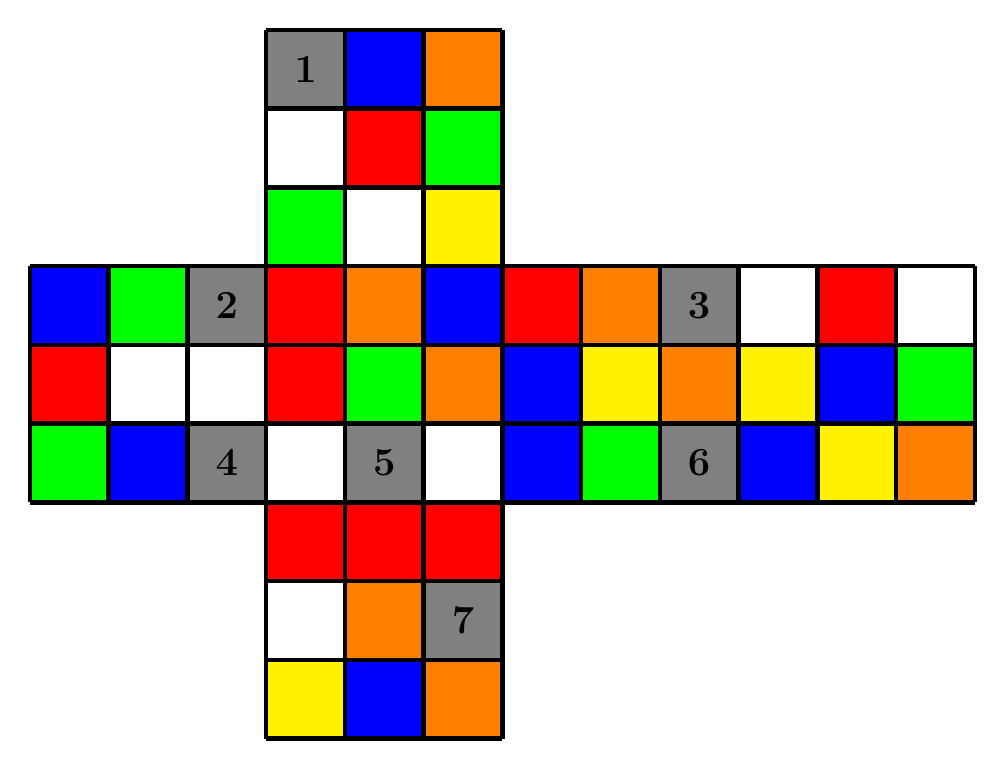
\begin{tikzpicture}[every node/.style={minimum size=1cm-\pgflinewidth, outer sep=0pt}]
\node[fill=gray] at (0.5,5.5) {\Large \textbf 1};
\node[fill=blue] at (1.5,5.5) {};
\node[fill=orange] at (2.5,5.5) {};
\node[fill=white] at (0.5,4.5) {};
\node[fill=red] at (1.5,4.5) {};
\node[fill=green] at (2.5,4.5) {};
\node[fill=green] at (0.5,3.5) {};
\node[fill=white] at (1.5,3.5) {};
\node[fill=yellow] at (2.5,3.5) {};

\node[fill=blue] at (-2.5,2.5) {};
\node[fill=green] at (-1.5,2.5) {};
\node[fill=gray] at (-0.5,2.5) {\Large \textbf 2};
\node[fill=red] at (0.5,2.5) {};
\node[fill=orange] at (1.5,2.5) {};
\node[fill=blue] at (2.5,2.5) {};
\node[fill=red] at (3.5,2.5) {};
\node[fill=orange] at (4.5,2.5) {};
\node[fill=gray] at (5.5,2.5) {\Large \textbf 3};
\node[fill=white] at (6.5,2.5) {};
\node[fill=red] at (7.5,2.5) {};
\node[fill=white] at (8.5,2.5) {};

\node[fill=red] at (-2.5,1.5) {};
\node[fill=white] at (-1.5,1.5) {};
\node[fill=white] at (-0.5,1.5) {};
\node[fill=red] at (0.5,1.5) {};
\node[fill=green] at (1.5,1.5) {};
\node[fill=orange] at (2.5,1.5) {};
\node[fill=blue] at (3.5,1.5) {};
\node[fill=yellow] at (4.5,1.5) {};
\node[fill=orange] at (5.5,1.5) {};
\node[fill=yellow] at (6.5,1.5) {};
\node[fill=blue] at (7.5,1.5) {};
\node[fill=green] at (8.5,1.5) {};

\node[fill=green] at (-2.5,0.5) {};
\node[fill=blue] at (-1.5,0.5) {};
\node[fill=gray] at (-0.5,0.5) {\Large \textbf 4};
\node[fill=white] at (0.5,0.5) {};
\node[fill=gray] at (1.5,0.5) {\Large \textbf 5};
\node[fill=white] at (2.5,0.5) {};
\node[fill=blue] at (3.5,0.5) {};
\node[fill=green] at (4.5,0.5) {};
\node[fill=gray] at (5.5,0.5) {\Large \textbf 6};
\node[fill=blue] at (6.5,0.5) {};
\node[fill=yellow] at (7.5,0.5) {};
\node[fill=orange] at (8.5,0.5) {};

\node[fill=red] at (0.5,-0.5) {};
\node[fill=red] at (1.5,-0.5) {};
\node[fill=red] at (2.5,-0.5) {};
\node[fill=white] at (0.5,-1.5) {};
\node[fill=orange] at (1.5,-1.5) {};
\node[fill=gray] at (2.5,-1.5) {\Large \textbf 7};
\node[fill=yellow] at (0.5,-2.5) {};
\node[fill=blue] at (1.5,-2.5) {};
\node[fill=orange] at (2.5,-2.5) {};

\draw[step=1cm,color=black, ultra thick] (-3,0) grid (9,3);
\draw[step=1cm,color=black, ultra thick] (0,-3) grid (3,0);
\draw[step=1cm,color=black, ultra thick] (0,3) grid (3,6);    
\end{tikzpicture}
\vspace{0.1cm}
\\
\noindent\normalsize \newtime  \textbf{Solution 47: D' U' B2 L2 D B2 U R2 U2 F2 U' R2 F D2 R' B' L2 U B D' Rw Uw}
\vspace{1cm}



{\noindent\Large \textbf{No. 48\qquad Difficulty:$\bigstar\bigstar$}}
\vspace{0.2cm}\\
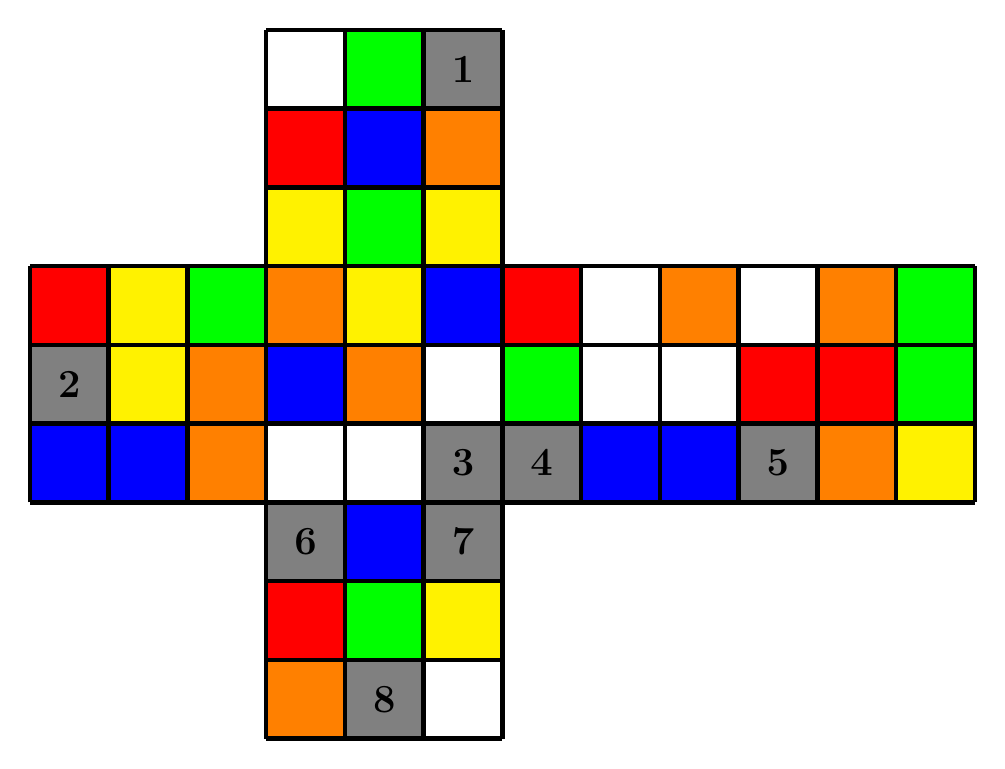
\begin{tikzpicture}[every node/.style={minimum size=1cm-\pgflinewidth, outer sep=0pt}]
\node[fill=white] at (0.5,5.5) {};
\node[fill=green] at (1.5,5.5) {};
\node[fill=gray] at (2.5,5.5) {\Large \textbf 1};
\node[fill=red] at (0.5,4.5) {};
\node[fill=blue] at (1.5,4.5) {};
\node[fill=orange] at (2.5,4.5) {};
\node[fill=yellow] at (0.5,3.5) {};
\node[fill=green] at (1.5,3.5) {};
\node[fill=yellow] at (2.5,3.5) {};

\node[fill=red] at (-2.5,2.5) {};
\node[fill=yellow] at (-1.5,2.5) {};
\node[fill=green] at (-0.5,2.5) {};
\node[fill=orange] at (0.5,2.5) {};
\node[fill=yellow] at (1.5,2.5) {};
\node[fill=blue] at (2.5,2.5) {};
\node[fill=red] at (3.5,2.5) {};
\node[fill=white] at (4.5,2.5) {};
\node[fill=orange] at (5.5,2.5) {};
\node[fill=white] at (6.5,2.5) {};
\node[fill=orange] at (7.5,2.5) {};
\node[fill=green] at (8.5,2.5) {};

\node[fill=gray] at (-2.5,1.5) {\Large \textbf 2};
\node[fill=yellow] at (-1.5,1.5) {};
\node[fill=orange] at (-0.5,1.5) {};
\node[fill=blue] at (0.5,1.5) {};
\node[fill=orange] at (1.5,1.5) {};
\node[fill=white] at (2.5,1.5) {};
\node[fill=green] at (3.5,1.5) {};
\node[fill=white] at (4.5,1.5) {};
\node[fill=white] at (5.5,1.5) {};
\node[fill=red] at (6.5,1.5) {};
\node[fill=red] at (7.5,1.5) {};
\node[fill=green] at (8.5,1.5) {};

\node[fill=blue] at (-2.5,0.5) {};
\node[fill=blue] at (-1.5,0.5) {};
\node[fill=orange] at (-0.5,0.5) {};
\node[fill=white] at (0.5,0.5) {};
\node[fill=white] at (1.5,0.5) {};
\node[fill=gray] at (2.5,0.5) {\Large \textbf 3};
\node[fill=gray] at (3.5,0.5) {\Large \textbf 4};
\node[fill=blue] at (4.5,0.5) {};
\node[fill=blue] at (5.5,0.5) {};
\node[fill=gray] at (6.5,0.5) {\Large \textbf 5};
\node[fill=orange] at (7.5,0.5) {};
\node[fill=yellow] at (8.5,0.5) {};

\node[fill=gray] at (0.5,-0.5) {\Large \textbf 6};
\node[fill=blue] at (1.5,-0.5) {};
\node[fill=gray] at (2.5,-0.5) {\Large \textbf 7};
\node[fill=red] at (0.5,-1.5) {};
\node[fill=green] at (1.5,-1.5) {};
\node[fill=yellow] at (2.5,-1.5) {};
\node[fill=orange] at (0.5,-2.5) {};
\node[fill=gray] at (1.5,-2.5) {\Large \textbf 8};
\node[fill=white] at (2.5,-2.5) {};

\draw[step=1cm,color=black, ultra thick] (-3,0) grid (9,3);
\draw[step=1cm,color=black, ultra thick] (0,-3) grid (3,0);
\draw[step=1cm,color=black, ultra thick] (0,3) grid (3,6);    
\end{tikzpicture}
\vspace{0.1cm}
\\
\noindent\normalsize \newtime  \textbf{Solution 48: R D L' U F2 D' B U F2 L D2 L' D2 L D2 F2 L' D2 L' D2 U' Fw Uw2}
\vspace{1cm}



{\noindent\Large \textbf{No. 49\qquad Difficulty:$\bigstar\bigstar$}}
\vspace{0.2cm}\\
\begin{tikzpicture}[every node/.style={minimum size=1cm-\pgflinewidth, outer sep=0pt}]
\node[fill=blue] at (0.5,5.5) {};
\node[fill=blue] at (1.5,5.5) {};
\node[fill=green] at (2.5,5.5) {};
\node[fill=yellow] at (0.5,4.5) {};
\node[fill=green] at (1.5,4.5) {};
\node[fill=white] at (2.5,4.5) {};
\node[fill=orange] at (0.5,3.5) {};
\node[fill=yellow] at (1.5,3.5) {};
\node[fill=gray] at (2.5,3.5) {\Large \textbf 1};

\node[fill=red] at (-2.5,2.5) {};
\node[fill=orange] at (-1.5,2.5) {};
\node[fill=blue] at (-0.5,2.5) {};
\node[fill=yellow] at (0.5,2.5) {};
\node[fill=red] at (1.5,2.5) {};
\node[fill=white] at (2.5,2.5) {};
\node[fill=orange] at (3.5,2.5) {};
\node[fill=orange] at (4.5,2.5) {};
\node[fill=yellow] at (5.5,2.5) {};
\node[fill=red] at (6.5,2.5) {};
\node[fill=white] at (7.5,2.5) {};
\node[fill=white] at (8.5,2.5) {};

\node[fill=orange] at (-2.5,1.5) {};
\node[fill=red] at (-1.5,1.5) {};
\node[fill=green] at (-0.5,1.5) {};
\node[fill=red] at (0.5,1.5) {};
\node[fill=white] at (1.5,1.5) {};
\node[fill=red] at (2.5,1.5) {};
\node[fill=white] at (3.5,1.5) {};
\node[fill=orange] at (4.5,1.5) {};
\node[fill=blue] at (5.5,1.5) {};
\node[fill=yellow] at (6.5,1.5) {};
\node[fill=yellow] at (7.5,1.5) {};
\node[fill=gray] at (8.5,1.5) {\Large \textbf 2};

\node[fill=blue] at (-2.5,0.5) {};
\node[fill=blue] at (-1.5,0.5) {};
\node[fill=green] at (-0.5,0.5) {};
\node[fill=gray] at (0.5,0.5) {\Large \textbf 3};
\node[fill=red] at (1.5,0.5) {};
\node[fill=yellow] at (2.5,0.5) {};
\node[fill=gray] at (3.5,0.5) {\Large \textbf 4};
\node[fill=white] at (4.5,0.5) {};
\node[fill=gray] at (5.5,0.5) {\Large \textbf 5};
\node[fill=yellow] at (6.5,0.5) {};
\node[fill=yellow] at (7.5,0.5) {};
\node[fill=orange] at (8.5,0.5) {};

\node[fill=red] at (0.5,-0.5) {};
\node[fill=blue] at (1.5,-0.5) {};
\node[fill=blue] at (2.5,-0.5) {};
\node[fill=orange] at (0.5,-1.5) {};
\node[fill=blue] at (1.5,-1.5) {};
\node[fill=green] at (2.5,-1.5) {};
\node[fill=white] at (0.5,-2.5) {};
\node[fill=gray] at (1.5,-2.5) {\Large \textbf 6};
\node[fill=gray] at (2.5,-2.5) {\Large \textbf 7};

\draw[step=1cm,color=black, ultra thick] (-3,0) grid (9,3);
\draw[step=1cm,color=black, ultra thick] (0,-3) grid (3,0);
\draw[step=1cm,color=black, ultra thick] (0,3) grid (3,6);    
\end{tikzpicture}
\vspace{0.1cm}
\\
\noindent\normalsize \newtime  \textbf{Solution 49: U2 F2 D2 U2 F' D2 R2 F D2 B L2 F' R' D L2 F' L' R' F' D2 L Fw' Uw}
\vspace{1cm}



{\noindent\Large \textbf{No. 50\qquad Difficulty:$\bigstar\bigstar$}}
\vspace{0.2cm}\\
\begin{tikzpicture}[every node/.style={minimum size=1cm-\pgflinewidth, outer sep=0pt}]
\node[fill=gray] at (0.5,5.5) {\Large \textbf 1};
\node[fill=green] at (1.5,5.5) {};
\node[fill=blue] at (2.5,5.5) {};
\node[fill=blue] at (0.5,4.5) {};
\node[fill=red] at (1.5,4.5) {};
\node[fill=blue] at (2.5,4.5) {};
\node[fill=yellow] at (0.5,3.5) {};
\node[fill=orange] at (1.5,3.5) {};
\node[fill=green] at (2.5,3.5) {};

\node[fill=yellow] at (-2.5,2.5) {};
\node[fill=yellow] at (-1.5,2.5) {};
\node[fill=blue] at (-0.5,2.5) {};
\node[fill=red] at (0.5,2.5) {};
\node[fill=green] at (1.5,2.5) {};
\node[fill=gray] at (2.5,2.5) {\Large \textbf 2};
\node[fill=orange] at (3.5,2.5) {};
\node[fill=white] at (4.5,2.5) {};
\node[fill=white] at (5.5,2.5) {};
\node[fill=gray] at (6.5,2.5) {\Large \textbf 3};
\node[fill=gray] at (7.5,2.5) {\Large \textbf 4};
\node[fill=gray] at (8.5,2.5) {\Large \textbf 5};

\node[fill=orange] at (-2.5,1.5) {};
\node[fill=blue] at (-1.5,1.5) {};
\node[fill=green] at (-0.5,1.5) {};
\node[fill=red] at (0.5,1.5) {};
\node[fill=white] at (1.5,1.5) {};
\node[fill=white] at (2.5,1.5) {};
\node[fill=red] at (3.5,1.5) {};
\node[fill=green] at (4.5,1.5) {};
\node[fill=gray] at (5.5,1.5) {\Large \textbf 6};
\node[fill=red] at (6.5,1.5) {};
\node[fill=yellow] at (7.5,1.5) {};
\node[fill=gray] at (8.5,1.5) {\Large \textbf 7};

\node[fill=green] at (-2.5,0.5) {};
\node[fill=yellow] at (-1.5,0.5) {};
\node[fill=gray] at (-0.5,0.5) {\Large \textbf 8};
\node[fill=gray] at (0.5,0.5) {\Large \textbf 9};
\node[fill=white] at (1.5,0.5) {};
\node[fill=gray] at (2.5,0.5) {\Large \textbf 10};
\node[fill=yellow] at (3.5,0.5) {};
\node[fill=blue] at (4.5,0.5) {};
\node[fill=orange] at (5.5,0.5) {};
\node[fill=gray] at (6.5,0.5) {\Large \textbf 11};
\node[fill=white] at (7.5,0.5) {};
\node[fill=red] at (8.5,0.5) {};

\node[fill=green] at (0.5,-0.5) {};
\node[fill=green] at (1.5,-0.5) {};
\node[fill=blue] at (2.5,-0.5) {};
\node[fill=red] at (0.5,-1.5) {};
\node[fill=orange] at (1.5,-1.5) {};
\node[fill=gray] at (2.5,-1.5) {\Large \textbf 12};
\node[fill=white] at (0.5,-2.5) {};
\node[fill=orange] at (1.5,-2.5) {};
\node[fill=white] at (2.5,-2.5) {};

\draw[step=1cm,color=black, ultra thick] (-3,0) grid (9,3);
\draw[step=1cm,color=black, ultra thick] (0,-3) grid (3,0);
\draw[step=1cm,color=black, ultra thick] (0,3) grid (3,6);    
\end{tikzpicture}
\vspace{0.1cm}
\\
\noindent\normalsize \newtime  \textbf{Solution 50: D L2 U' R2 D2 L2 R2 F2 U B2 U F2 B' L' U' B D U' L2 D' F2 Rw}
\vspace{1cm}



{\noindent\Large \textbf{No. 51\qquad Difficulty:$\bigstar\bigstar\bigstar$}}
\vspace{0.2cm}\\
\begin{tikzpicture}[every node/.style={minimum size=1cm-\pgflinewidth, outer sep=0pt}]
\node[fill=gray] at (0.5,5.5) {\Large \textbf 1};
\node[fill=white] at (1.5,5.5) {};
\node[fill=gray] at (2.5,5.5) {\Large \textbf 2};
\node[fill=gray] at (0.5,4.5) {\Large \textbf 3};
\node[fill=orange] at (1.5,4.5) {};
\node[fill=yellow] at (2.5,4.5) {};
\node[fill=white] at (0.5,3.5) {};
\node[fill=green] at (1.5,3.5) {};
\node[fill=yellow] at (2.5,3.5) {};

\node[fill=white] at (-2.5,2.5) {};
\node[fill=white] at (-1.5,2.5) {};
\node[fill=orange] at (-0.5,2.5) {};
\node[fill=gray] at (0.5,2.5) {\Large \textbf 4};
\node[fill=orange] at (1.5,2.5) {};
\node[fill=gray] at (2.5,2.5) {\Large \textbf 5};
\node[fill=orange] at (3.5,2.5) {};
\node[fill=gray] at (4.5,2.5) {\Large \textbf 6};
\node[fill=white] at (5.5,2.5) {};
\node[fill=green] at (6.5,2.5) {};
\node[fill=green] at (7.5,2.5) {};
\node[fill=gray] at (8.5,2.5) {\Large \textbf 7};

\node[fill=blue] at (-2.5,1.5) {};
\node[fill=white] at (-1.5,1.5) {};
\node[fill=green] at (-0.5,1.5) {};
\node[fill=yellow] at (0.5,1.5) {};
\node[fill=blue] at (1.5,1.5) {};
\node[fill=gray] at (2.5,1.5) {\Large \textbf 8};
\node[fill=gray] at (3.5,1.5) {\Large \textbf 9};
\node[fill=yellow] at (4.5,1.5) {};
\node[fill=white] at (5.5,1.5) {};
\node[fill=red] at (6.5,1.5) {};
\node[fill=green] at (7.5,1.5) {};
\node[fill=red] at (8.5,1.5) {};

\node[fill=yellow] at (-2.5,0.5) {};
\node[fill=orange] at (-1.5,0.5) {};
\node[fill=blue] at (-0.5,0.5) {};
\node[fill=gray] at (0.5,0.5) {\Large \textbf 10};
\node[fill=orange] at (1.5,0.5) {};
\node[fill=orange] at (2.5,0.5) {};
\node[fill=yellow] at (3.5,0.5) {};
\node[fill=blue] at (4.5,0.5) {};
\node[fill=blue] at (5.5,0.5) {};
\node[fill=gray] at (6.5,0.5) {\Large \textbf 11};
\node[fill=yellow] at (7.5,0.5) {};
\node[fill=red] at (8.5,0.5) {};

\node[fill=gray] at (0.5,-0.5) {\Large \textbf 12};
\node[fill=blue] at (1.5,-0.5) {};
\node[fill=gray] at (2.5,-0.5) {\Large \textbf 13};
\node[fill=yellow] at (0.5,-1.5) {};
\node[fill=red] at (1.5,-1.5) {};
\node[fill=white] at (2.5,-1.5) {};
\node[fill=gray] at (0.5,-2.5) {\Large \textbf 14};
\node[fill=blue] at (1.5,-2.5) {};
\node[fill=white] at (2.5,-2.5) {};

\draw[step=1cm,color=black, ultra thick] (-3,0) grid (9,3);
\draw[step=1cm,color=black, ultra thick] (0,-3) grid (3,0);
\draw[step=1cm,color=black, ultra thick] (0,3) grid (3,6);    
\end{tikzpicture}
\vspace{0.1cm}
\\
\noindent\normalsize \newtime  \textbf{Solution 51: B2 D2 R2 D' L2 B2 U L2 R2 D2 L2 U' F R' U B2 D L2 B2 L2 B' Rw' Uw'}
\vspace{1cm}



{\noindent\Large \textbf{No. 52\qquad Difficulty:$\bigstar\bigstar\bigstar$}}
\vspace{0.2cm}\\
\begin{tikzpicture}[every node/.style={minimum size=1cm-\pgflinewidth, outer sep=0pt}]
\node[fill=green] at (0.5,5.5) {};
\node[fill=green] at (1.5,5.5) {};
\node[fill=yellow] at (2.5,5.5) {};
\node[fill=gray] at (0.5,4.5) {\Large \textbf 1};
\node[fill=blue] at (1.5,4.5) {};
\node[fill=red] at (2.5,4.5) {};
\node[fill=gray] at (0.5,3.5) {\Large \textbf 2};
\node[fill=green] at (1.5,3.5) {};
\node[fill=red] at (2.5,3.5) {};

\node[fill=gray] at (-2.5,2.5) {\Large \textbf 3};
\node[fill=white] at (-1.5,2.5) {};
\node[fill=red] at (-0.5,2.5) {};
\node[fill=green] at (0.5,2.5) {};
\node[fill=yellow] at (1.5,2.5) {};
\node[fill=yellow] at (2.5,2.5) {};
\node[fill=gray] at (3.5,2.5) {\Large \textbf 4};
\node[fill=yellow] at (4.5,2.5) {};
\node[fill=gray] at (5.5,2.5) {\Large \textbf 5};
\node[fill=orange] at (6.5,2.5) {};
\node[fill=red] at (7.5,2.5) {};
\node[fill=gray] at (8.5,2.5) {\Large \textbf 6};

\node[fill=green] at (-2.5,1.5) {};
\node[fill=orange] at (-1.5,1.5) {};
\node[fill=blue] at (-0.5,1.5) {};
\node[fill=orange] at (0.5,1.5) {};
\node[fill=white] at (1.5,1.5) {};
\node[fill=green] at (2.5,1.5) {};
\node[fill=gray] at (3.5,1.5) {\Large \textbf 7};
\node[fill=red] at (4.5,1.5) {};
\node[fill=orange] at (5.5,1.5) {};
\node[fill=yellow] at (6.5,1.5) {};
\node[fill=yellow] at (7.5,1.5) {};
\node[fill=orange] at (8.5,1.5) {};

\node[fill=gray] at (-2.5,0.5) {\Large \textbf 8};
\node[fill=yellow] at (-1.5,0.5) {};
\node[fill=white] at (-0.5,0.5) {};
\node[fill=orange] at (0.5,0.5) {};
\node[fill=white] at (1.5,0.5) {};
\node[fill=yellow] at (2.5,0.5) {};
\node[fill=blue] at (3.5,0.5) {};
\node[fill=red] at (4.5,0.5) {};
\node[fill=red] at (5.5,0.5) {};
\node[fill=green] at (6.5,0.5) {};
\node[fill=orange] at (7.5,0.5) {};
\node[fill=gray] at (8.5,0.5) {\Large \textbf 9};

\node[fill=gray] at (0.5,-0.5) {\Large \textbf 10};
\node[fill=blue] at (1.5,-0.5) {};
\node[fill=gray] at (2.5,-0.5) {\Large \textbf 11};
\node[fill=gray] at (0.5,-1.5) {\Large \textbf 12};
\node[fill=green] at (1.5,-1.5) {};
\node[fill=blue] at (2.5,-1.5) {};
\node[fill=gray] at (0.5,-2.5) {\Large \textbf 13};
\node[fill=white] at (1.5,-2.5) {};
\node[fill=white] at (2.5,-2.5) {};

\draw[step=1cm,color=black, ultra thick] (-3,0) grid (9,3);
\draw[step=1cm,color=black, ultra thick] (0,-3) grid (3,0);
\draw[step=1cm,color=black, ultra thick] (0,3) grid (3,6);    
\end{tikzpicture}
\vspace{0.1cm}
\\
\noindent\normalsize \newtime  \textbf{Solution 52: R D2 B R2 L2 B2 R U D2 B2 U2 R2 U2 B' R2 B' U2 F D2 R2 L Fw Uw'}
\vspace{1cm}



{\noindent\Large \textbf{No. 53\qquad Difficulty:$\bigstar\bigstar\bigstar$}}
\vspace{0.2cm}\\
\begin{tikzpicture}[every node/.style={minimum size=1cm-\pgflinewidth, outer sep=0pt}]
\node[fill=gray] at (0.5,5.5) {\Large \textbf 1};
\node[fill=gray] at (1.5,5.5) {\Large \textbf 2};
\node[fill=gray] at (2.5,5.5) {\Large \textbf 3};
\node[fill=yellow] at (0.5,4.5) {};
\node[fill=green] at (1.5,4.5) {};
\node[fill=white] at (2.5,4.5) {};
\node[fill=orange] at (0.5,3.5) {};
\node[fill=blue] at (1.5,3.5) {};
\node[fill=white] at (2.5,3.5) {};

\node[fill=yellow] at (-2.5,2.5) {};
\node[fill=gray] at (-1.5,2.5) {\Large \textbf 4};
\node[fill=white] at (-0.5,2.5) {};
\node[fill=blue] at (0.5,2.5) {};
\node[fill=white] at (1.5,2.5) {};
\node[fill=gray] at (2.5,2.5) {\Large \textbf 5};
\node[fill=blue] at (3.5,2.5) {};
\node[fill=green] at (4.5,2.5) {};
\node[fill=gray] at (5.5,2.5) {\Large \textbf 6};
\node[fill=white] at (6.5,2.5) {};
\node[fill=red] at (7.5,2.5) {};
\node[fill=gray] at (8.5,2.5) {\Large \textbf 7};

\node[fill=red] at (-2.5,1.5) {};
\node[fill=red] at (-1.5,1.5) {};
\node[fill=gray] at (-0.5,1.5) {\Large \textbf 8};
\node[fill=orange] at (0.5,1.5) {};
\node[fill=white] at (1.5,1.5) {};
\node[fill=white] at (2.5,1.5) {};
\node[fill=gray] at (3.5,1.5) {\Large \textbf 9};
\node[fill=orange] at (4.5,1.5) {};
\node[fill=red] at (5.5,1.5) {};
\node[fill=green] at (6.5,1.5) {};
\node[fill=yellow] at (7.5,1.5) {};
\node[fill=white] at (8.5,1.5) {};

\node[fill=red] at (-2.5,0.5) {};
\node[fill=blue] at (-1.5,0.5) {};
\node[fill=gray] at (-0.5,0.5) {\Large \textbf 10};
\node[fill=yellow] at (0.5,0.5) {};
\node[fill=gray] at (1.5,0.5) {\Large \textbf 11};
\node[fill=gray] at (2.5,0.5) {\Large \textbf 12};
\node[fill=red] at (3.5,0.5) {};
\node[fill=blue] at (4.5,0.5) {};
\node[fill=yellow] at (5.5,0.5) {};
\node[fill=green] at (6.5,0.5) {};
\node[fill=red] at (7.5,0.5) {};
\node[fill=yellow] at (8.5,0.5) {};

\node[fill=orange] at (0.5,-0.5) {};
\node[fill=green] at (1.5,-0.5) {};
\node[fill=green] at (2.5,-0.5) {};
\node[fill=yellow] at (0.5,-1.5) {};
\node[fill=blue] at (1.5,-1.5) {};
\node[fill=orange] at (2.5,-1.5) {};
\node[fill=gray] at (0.5,-2.5) {\Large \textbf 13};
\node[fill=yellow] at (1.5,-2.5) {};
\node[fill=red] at (2.5,-2.5) {};

\draw[step=1cm,color=black, ultra thick] (-3,0) grid (9,3);
\draw[step=1cm,color=black, ultra thick] (0,-3) grid (3,0);
\draw[step=1cm,color=black, ultra thick] (0,3) grid (3,6);    
\end{tikzpicture}
\vspace{0.1cm}
\\
\noindent\normalsize \newtime  \textbf{Solution 53: B2 R' B2 U2 R' D2 L F R2 D L2 F2 D' B2 D' B2 R2 U' B2 L2 Fw' Uw}
\vspace{1cm}



{\noindent\Large \textbf{No. 54\qquad Difficulty:$\bigstar\bigstar\bigstar$}}
\vspace{0.2cm}\\
\begin{tikzpicture}[every node/.style={minimum size=1cm-\pgflinewidth, outer sep=0pt}]
\node[fill=green] at (0.5,5.5) {};
\node[fill=orange] at (1.5,5.5) {};
\node[fill=green] at (2.5,5.5) {};
\node[fill=white] at (0.5,4.5) {};
\node[fill=red] at (1.5,4.5) {};
\node[fill=yellow] at (2.5,4.5) {};
\node[fill=blue] at (0.5,3.5) {};
\node[fill=green] at (1.5,3.5) {};
\node[fill=gray] at (2.5,3.5) {\Large \textbf 1};

\node[fill=gray] at (-2.5,2.5) {\Large \textbf 2};
\node[fill=gray] at (-1.5,2.5) {\Large \textbf 3};
\node[fill=white] at (-0.5,2.5) {};
\node[fill=gray] at (0.5,2.5) {\Large \textbf 4};
\node[fill=yellow] at (1.5,2.5) {};
\node[fill=blue] at (2.5,2.5) {};
\node[fill=gray] at (3.5,2.5) {\Large \textbf 5};
\node[fill=orange] at (4.5,2.5) {};
\node[fill=gray] at (5.5,2.5) {\Large \textbf 6};
\node[fill=yellow] at (6.5,2.5) {};
\node[fill=blue] at (7.5,2.5) {};
\node[fill=white] at (8.5,2.5) {};

\node[fill=red] at (-2.5,1.5) {};
\node[fill=green] at (-1.5,1.5) {};
\node[fill=red] at (-0.5,1.5) {};
\node[fill=blue] at (0.5,1.5) {};
\node[fill=yellow] at (1.5,1.5) {};
\node[fill=white] at (2.5,1.5) {};
\node[fill=green] at (3.5,1.5) {};
\node[fill=blue] at (4.5,1.5) {};
\node[fill=white] at (5.5,1.5) {};
\node[fill=blue] at (6.5,1.5) {};
\node[fill=white] at (7.5,1.5) {};
\node[fill=white] at (8.5,1.5) {};

\node[fill=gray] at (-2.5,0.5) {\Large \textbf 7};
\node[fill=gray] at (-1.5,0.5) {\Large \textbf 8};
\node[fill=red] at (-0.5,0.5) {};
\node[fill=gray] at (0.5,0.5) {\Large \textbf 9};
\node[fill=red] at (1.5,0.5) {};
\node[fill=orange] at (2.5,0.5) {};
\node[fill=blue] at (3.5,0.5) {};
\node[fill=gray] at (4.5,0.5) {\Large \textbf 10};
\node[fill=red] at (5.5,0.5) {};
\node[fill=gray] at (6.5,0.5) {\Large \textbf 11};
\node[fill=orange] at (7.5,0.5) {};
\node[fill=orange] at (8.5,0.5) {};

\node[fill=white] at (0.5,-0.5) {};
\node[fill=yellow] at (1.5,-0.5) {};
\node[fill=gray] at (2.5,-0.5) {\Large \textbf 12};
\node[fill=gray] at (0.5,-1.5) {\Large \textbf 13};
\node[fill=orange] at (1.5,-1.5) {};
\node[fill=yellow] at (2.5,-1.5) {};
\node[fill=blue] at (0.5,-2.5) {};
\node[fill=green] at (1.5,-2.5) {};
\node[fill=gray] at (2.5,-2.5) {\Large \textbf 14};

\draw[step=1cm,color=black, ultra thick] (-3,0) grid (9,3);
\draw[step=1cm,color=black, ultra thick] (0,-3) grid (3,0);
\draw[step=1cm,color=black, ultra thick] (0,3) grid (3,6);    
\end{tikzpicture}
\vspace{0.1cm}
\\
\noindent\normalsize \newtime  \textbf{Solution 54: R' F' R2 F' L2 B' R2 D2 L2 R2 B2 D2 F' D B' R' D R2 D L2 U' Rw Uw2}
\vspace{1cm}



{\noindent\Large \textbf{No. 55\qquad Difficulty:$\bigstar\bigstar\bigstar$}}
\vspace{0.2cm}\\
\begin{tikzpicture}[every node/.style={minimum size=1cm-\pgflinewidth, outer sep=0pt}]
\node[fill=white] at (0.5,5.5) {};
\node[fill=green] at (1.5,5.5) {};
\node[fill=gray] at (2.5,5.5) {\Large \textbf 1};
\node[fill=yellow] at (0.5,4.5) {};
\node[fill=orange] at (1.5,4.5) {};
\node[fill=yellow] at (2.5,4.5) {};
\node[fill=yellow] at (0.5,3.5) {};
\node[fill=gray] at (1.5,3.5) {\Large \textbf 2};
\node[fill=blue] at (2.5,3.5) {};

\node[fill=gray] at (-2.5,2.5) {\Large \textbf 3};
\node[fill=red] at (-1.5,2.5) {};
\node[fill=red] at (-0.5,2.5) {};
\node[fill=gray] at (0.5,2.5) {\Large \textbf 4};
\node[fill=red] at (1.5,2.5) {};
\node[fill=red] at (2.5,2.5) {};
\node[fill=gray] at (3.5,2.5) {\Large \textbf 5};
\node[fill=blue] at (4.5,2.5) {};
\node[fill=gray] at (5.5,2.5) {\Large \textbf 6};
\node[fill=gray] at (6.5,2.5) {\Large \textbf 7};
\node[fill=orange] at (7.5,2.5) {};
\node[fill=orange] at (8.5,2.5) {};

\node[fill=orange] at (-2.5,1.5) {};
\node[fill=white] at (-1.5,1.5) {};
\node[fill=white] at (-0.5,1.5) {};
\node[fill=green] at (0.5,1.5) {};
\node[fill=blue] at (1.5,1.5) {};
\node[fill=red] at (2.5,1.5) {};
\node[fill=blue] at (3.5,1.5) {};
\node[fill=yellow] at (4.5,1.5) {};
\node[fill=green] at (5.5,1.5) {};
\node[fill=yellow] at (6.5,1.5) {};
\node[fill=green] at (7.5,1.5) {};
\node[fill=yellow] at (8.5,1.5) {};

\node[fill=white] at (-2.5,0.5) {};
\node[fill=gray] at (-1.5,0.5) {\Large \textbf 8};
\node[fill=yellow] at (-0.5,0.5) {};
\node[fill=gray] at (0.5,0.5) {\Large \textbf 9};
\node[fill=gray] at (1.5,0.5) {\Large \textbf 10};
\node[fill=green] at (2.5,0.5) {};
\node[fill=white] at (3.5,0.5) {};
\node[fill=white] at (4.5,0.5) {};
\node[fill=blue] at (5.5,0.5) {};
\node[fill=white] at (6.5,0.5) {};
\node[fill=orange] at (7.5,0.5) {};
\node[fill=red] at (8.5,0.5) {};

\node[fill=green] at (0.5,-0.5) {};
\node[fill=blue] at (1.5,-0.5) {};
\node[fill=gray] at (2.5,-0.5) {\Large \textbf 11};
\node[fill=white] at (0.5,-1.5) {};
\node[fill=red] at (1.5,-1.5) {};
\node[fill=red] at (2.5,-1.5) {};
\node[fill=gray] at (0.5,-2.5) {\Large \textbf 12};
\node[fill=gray] at (1.5,-2.5) {\Large \textbf 13};
\node[fill=gray] at (2.5,-2.5) {\Large \textbf 14};

\draw[step=1cm,color=black, ultra thick] (-3,0) grid (9,3);
\draw[step=1cm,color=black, ultra thick] (0,-3) grid (3,0);
\draw[step=1cm,color=black, ultra thick] (0,3) grid (3,6);    
\end{tikzpicture}
\vspace{0.1cm}
\\
\noindent\normalsize \newtime  \textbf{Solution 55: F' B2 D' L U B' D' F U2 R' F2 D2 B2 U2 L2 D2 R' F2 U2 L F Rw' Uw'}
\vspace{1cm}



{\noindent\Large \textbf{No. 56\qquad Difficulty:$\bigstar\bigstar\bigstar$}}
\vspace{0.2cm}\\
\begin{tikzpicture}[every node/.style={minimum size=1cm-\pgflinewidth, outer sep=0pt}]
\node[fill=gray] at (0.5,5.5) {\Large \textbf 1};
\node[fill=orange] at (1.5,5.5) {};
\node[fill=green] at (2.5,5.5) {};
\node[fill=blue] at (0.5,4.5) {};
\node[fill=red] at (1.5,4.5) {};
\node[fill=red] at (2.5,4.5) {};
\node[fill=gray] at (0.5,3.5) {\Large \textbf 2};
\node[fill=white] at (1.5,3.5) {};
\node[fill=blue] at (2.5,3.5) {};

\node[fill=gray] at (-2.5,2.5) {\Large \textbf 3};
\node[fill=gray] at (-1.5,2.5) {\Large \textbf 4};
\node[fill=yellow] at (-0.5,2.5) {};
\node[fill=gray] at (0.5,2.5) {\Large \textbf 5};
\node[fill=gray] at (1.5,2.5) {\Large \textbf 6};
\node[fill=orange] at (2.5,2.5) {};
\node[fill=white] at (3.5,2.5) {};
\node[fill=blue] at (4.5,2.5) {};
\node[fill=white] at (5.5,2.5) {};
\node[fill=gray] at (6.5,2.5) {\Large \textbf 7};
\node[fill=gray] at (7.5,2.5) {\Large \textbf 8};
\node[fill=green] at (8.5,2.5) {};

\node[fill=yellow] at (-2.5,1.5) {};
\node[fill=yellow] at (-1.5,1.5) {};
\node[fill=gray] at (-0.5,1.5) {\Large \textbf 9};
\node[fill=green] at (0.5,1.5) {};
\node[fill=blue] at (1.5,1.5) {};
\node[fill=yellow] at (2.5,1.5) {};
\node[fill=orange] at (3.5,1.5) {};
\node[fill=white] at (4.5,1.5) {};
\node[fill=yellow] at (5.5,1.5) {};
\node[fill=green] at (6.5,1.5) {};
\node[fill=green] at (7.5,1.5) {};
\node[fill=red] at (8.5,1.5) {};

\node[fill=red] at (-2.5,0.5) {};
\node[fill=orange] at (-1.5,0.5) {};
\node[fill=gray] at (-0.5,0.5) {\Large \textbf 10};
\node[fill=blue] at (0.5,0.5) {};
\node[fill=orange] at (1.5,0.5) {};
\node[fill=blue] at (2.5,0.5) {};
\node[fill=gray] at (3.5,0.5) {\Large \textbf 11};
\node[fill=blue] at (4.5,0.5) {};
\node[fill=gray] at (5.5,0.5) {\Large \textbf 12};
\node[fill=green] at (6.5,0.5) {};
\node[fill=red] at (7.5,0.5) {};
\node[fill=green] at (8.5,0.5) {};

\node[fill=red] at (0.5,-0.5) {};
\node[fill=blue] at (1.5,-0.5) {};
\node[fill=gray] at (2.5,-0.5) {\Large \textbf 13};
\node[fill=white] at (0.5,-1.5) {};
\node[fill=orange] at (1.5,-1.5) {};
\node[fill=white] at (2.5,-1.5) {};
\node[fill=yellow] at (0.5,-2.5) {};
\node[fill=green] at (1.5,-2.5) {};
\node[fill=yellow] at (2.5,-2.5) {};

\draw[step=1cm,color=black, ultra thick] (-3,0) grid (9,3);
\draw[step=1cm,color=black, ultra thick] (0,-3) grid (3,0);
\draw[step=1cm,color=black, ultra thick] (0,3) grid (3,6);    
\end{tikzpicture}
\vspace{0.1cm}
\\
\noindent\normalsize \newtime  \textbf{Solution 56: R D2 R2 F U2 F L' F2 U R2 F2 D' L2 U R2 B2 L2 B2 U2 Rw Uw'}
\vspace{1cm}



{\noindent\Large \textbf{No. 57\qquad Difficulty:$\bigstar\bigstar\bigstar$}}
\vspace{0.2cm}\\
\begin{tikzpicture}[every node/.style={minimum size=1cm-\pgflinewidth, outer sep=0pt}]
\node[fill=yellow] at (0.5,5.5) {};
\node[fill=yellow] at (1.5,5.5) {};
\node[fill=gray] at (2.5,5.5) {\Large \textbf 1};
\node[fill=orange] at (0.5,4.5) {};
\node[fill=blue] at (1.5,4.5) {};
\node[fill=yellow] at (2.5,4.5) {};
\node[fill=gray] at (0.5,3.5) {\Large \textbf 2};
\node[fill=orange] at (1.5,3.5) {};
\node[fill=blue] at (2.5,3.5) {};

\node[fill=blue] at (-2.5,2.5) {};
\node[fill=gray] at (-1.5,2.5) {\Large \textbf 3};
\node[fill=gray] at (-0.5,2.5) {\Large \textbf 4};
\node[fill=yellow] at (0.5,2.5) {};
\node[fill=blue] at (1.5,2.5) {};
\node[fill=white] at (2.5,2.5) {};
\node[fill=red] at (3.5,2.5) {};
\node[fill=gray] at (4.5,2.5) {\Large \textbf 5};
\node[fill=white] at (5.5,2.5) {};
\node[fill=gray] at (6.5,2.5) {\Large \textbf 6};
\node[fill=blue] at (7.5,2.5) {};
\node[fill=orange] at (8.5,2.5) {};

\node[fill=orange] at (-2.5,1.5) {};
\node[fill=orange] at (-1.5,1.5) {};
\node[fill=gray] at (-0.5,1.5) {\Large \textbf 7};
\node[fill=red] at (0.5,1.5) {};
\node[fill=white] at (1.5,1.5) {};
\node[fill=white] at (2.5,1.5) {};
\node[fill=blue] at (3.5,1.5) {};
\node[fill=red] at (4.5,1.5) {};
\node[fill=gray] at (5.5,1.5) {\Large \textbf 8};
\node[fill=white] at (6.5,1.5) {};
\node[fill=yellow] at (7.5,1.5) {};
\node[fill=green] at (8.5,1.5) {};

\node[fill=blue] at (-2.5,0.5) {};
\node[fill=blue] at (-1.5,0.5) {};
\node[fill=gray] at (-0.5,0.5) {\Large \textbf 9};
\node[fill=orange] at (0.5,0.5) {};
\node[fill=orange] at (1.5,0.5) {};
\node[fill=orange] at (2.5,0.5) {};
\node[fill=gray] at (3.5,0.5) {\Large \textbf 10};
\node[fill=yellow] at (4.5,0.5) {};
\node[fill=gray] at (5.5,0.5) {\Large \textbf 11};
\node[fill=green] at (6.5,0.5) {};
\node[fill=white] at (7.5,0.5) {};
\node[fill=gray] at (8.5,0.5) {\Large \textbf 12};

\node[fill=green] at (0.5,-0.5) {};
\node[fill=yellow] at (1.5,-0.5) {};
\node[fill=gray] at (2.5,-0.5) {\Large \textbf 13};
\node[fill=gray] at (0.5,-1.5) {\Large \textbf 14};
\node[fill=green] at (1.5,-1.5) {};
\node[fill=green] at (2.5,-1.5) {};
\node[fill=gray] at (0.5,-2.5) {\Large \textbf 15};
\node[fill=green] at (1.5,-2.5) {};
\node[fill=red] at (2.5,-2.5) {};

\draw[step=1cm,color=black, ultra thick] (-3,0) grid (9,3);
\draw[step=1cm,color=black, ultra thick] (0,-3) grid (3,0);
\draw[step=1cm,color=black, ultra thick] (0,3) grid (3,6);    
\end{tikzpicture}
\vspace{0.1cm}
\\
\noindent\normalsize \newtime  \textbf{Solution 57: R2 B' R D2 L D R2 F' R U' B2 U L2 D' F2 U R2 U2 L2 B2 D2 Fw Uw'}
\vspace{1cm}



{\noindent\Large \textbf{No. 58\qquad Difficulty:$\bigstar\bigstar\bigstar$}}
\vspace{0.2cm}\\
\begin{tikzpicture}[every node/.style={minimum size=1cm-\pgflinewidth, outer sep=0pt}]
\node[fill=orange] at (0.5,5.5) {};
\node[fill=red] at (1.5,5.5) {};
\node[fill=gray] at (2.5,5.5) {\Large \textbf 1};
\node[fill=gray] at (0.5,4.5) {\Large \textbf 2};
\node[fill=red] at (1.5,4.5) {};
\node[fill=white] at (2.5,4.5) {};
\node[fill=gray] at (0.5,3.5) {\Large \textbf 3};
\node[fill=orange] at (1.5,3.5) {};
\node[fill=white] at (2.5,3.5) {};

\node[fill=white] at (-2.5,2.5) {};
\node[fill=red] at (-1.5,2.5) {};
\node[fill=green] at (-0.5,2.5) {};
\node[fill=orange] at (0.5,2.5) {};
\node[fill=yellow] at (1.5,2.5) {};
\node[fill=green] at (2.5,2.5) {};
\node[fill=red] at (3.5,2.5) {};
\node[fill=orange] at (4.5,2.5) {};
\node[fill=gray] at (5.5,2.5) {\Large \textbf 4};
\node[fill=gray] at (6.5,2.5) {\Large \textbf 5};
\node[fill=white] at (7.5,2.5) {};
\node[fill=gray] at (8.5,2.5) {\Large \textbf 6};

\node[fill=gray] at (-2.5,1.5) {\Large \textbf 7};
\node[fill=yellow] at (-1.5,1.5) {};
\node[fill=yellow] at (-0.5,1.5) {};
\node[fill=green] at (0.5,1.5) {};
\node[fill=blue] at (1.5,1.5) {};
\node[fill=red] at (2.5,1.5) {};
\node[fill=green] at (3.5,1.5) {};
\node[fill=white] at (4.5,1.5) {};
\node[fill=green] at (5.5,1.5) {};
\node[fill=white] at (6.5,1.5) {};
\node[fill=green] at (7.5,1.5) {};
\node[fill=yellow] at (8.5,1.5) {};

\node[fill=gray] at (-2.5,0.5) {\Large \textbf 8};
\node[fill=blue] at (-1.5,0.5) {};
\node[fill=orange] at (-0.5,0.5) {};
\node[fill=gray] at (0.5,0.5) {\Large \textbf 9};
\node[fill=green] at (1.5,0.5) {};
\node[fill=red] at (2.5,0.5) {};
\node[fill=white] at (3.5,0.5) {};
\node[fill=orange] at (4.5,0.5) {};
\node[fill=green] at (5.5,0.5) {};
\node[fill=gray] at (6.5,0.5) {\Large \textbf 10};
\node[fill=gray] at (7.5,0.5) {\Large \textbf 11};
\node[fill=white] at (8.5,0.5) {};

\node[fill=gray] at (0.5,-0.5) {\Large \textbf 12};
\node[fill=orange] at (1.5,-0.5) {};
\node[fill=blue] at (2.5,-0.5) {};
\node[fill=gray] at (0.5,-1.5) {\Large \textbf 13};
\node[fill=orange] at (1.5,-1.5) {};
\node[fill=blue] at (2.5,-1.5) {};
\node[fill=blue] at (0.5,-2.5) {};
\node[fill=white] at (1.5,-2.5) {};
\node[fill=gray] at (2.5,-2.5) {\Large \textbf 14};

\draw[step=1cm,color=black, ultra thick] (-3,0) grid (9,3);
\draw[step=1cm,color=black, ultra thick] (0,-3) grid (3,0);
\draw[step=1cm,color=black, ultra thick] (0,3) grid (3,6);    
\end{tikzpicture}
\vspace{0.1cm}
\\
\noindent\normalsize \newtime  \textbf{Solution 58: D2 L' B D2 B' F2 U2 L2 F D2 L2 F U2 L D' U' R' D' R B' L Rw Uw'}
\vspace{1cm}



{\noindent\Large \textbf{No. 59\qquad Difficulty:$\bigstar\bigstar\bigstar$}}
\vspace{0.2cm}\\
\begin{tikzpicture}[every node/.style={minimum size=1cm-\pgflinewidth, outer sep=0pt}]
\node[fill=gray] at (0.5,5.5) {\Large \textbf 1};
\node[fill=blue] at (1.5,5.5) {};
\node[fill=red] at (2.5,5.5) {};
\node[fill=blue] at (0.5,4.5) {};
\node[fill=green] at (1.5,4.5) {};
\node[fill=gray] at (2.5,4.5) {\Large \textbf 2};
\node[fill=green] at (0.5,3.5) {};
\node[fill=red] at (1.5,3.5) {};
\node[fill=red] at (2.5,3.5) {};

\node[fill=green] at (-2.5,2.5) {};
\node[fill=red] at (-1.5,2.5) {};
\node[fill=gray] at (-0.5,2.5) {\Large \textbf 3};
\node[fill=gray] at (0.5,2.5) {\Large \textbf 4};
\node[fill=green] at (1.5,2.5) {};
\node[fill=white] at (2.5,2.5) {};
\node[fill=green] at (3.5,2.5) {};
\node[fill=red] at (4.5,2.5) {};
\node[fill=blue] at (5.5,2.5) {};
\node[fill=white] at (6.5,2.5) {};
\node[fill=yellow] at (7.5,2.5) {};
\node[fill=red] at (8.5,2.5) {};

\node[fill=yellow] at (-2.5,1.5) {};
\node[fill=orange] at (-1.5,1.5) {};
\node[fill=blue] at (-0.5,1.5) {};
\node[fill=white] at (0.5,1.5) {};
\node[fill=yellow] at (1.5,1.5) {};
\node[fill=gray] at (2.5,1.5) {\Large \textbf 5};
\node[fill=yellow] at (3.5,1.5) {};
\node[fill=red] at (4.5,1.5) {};
\node[fill=gray] at (5.5,1.5) {\Large \textbf 6};
\node[fill=green] at (6.5,1.5) {};
\node[fill=white] at (7.5,1.5) {};
\node[fill=orange] at (8.5,1.5) {};

\node[fill=gray] at (-2.5,0.5) {\Large \textbf 7};
\node[fill=green] at (-1.5,0.5) {};
\node[fill=orange] at (-0.5,0.5) {};
\node[fill=gray] at (0.5,0.5) {\Large \textbf 8};
\node[fill=orange] at (1.5,0.5) {};
\node[fill=blue] at (2.5,0.5) {};
\node[fill=gray] at (3.5,0.5) {\Large \textbf 9};
\node[fill=gray] at (4.5,0.5) {\Large \textbf 10};
\node[fill=orange] at (5.5,0.5) {};
\node[fill=gray] at (6.5,0.5) {\Large \textbf 11};
\node[fill=green] at (7.5,0.5) {};
\node[fill=gray] at (8.5,0.5) {\Large \textbf 12};

\node[fill=yellow] at (0.5,-0.5) {};
\node[fill=blue] at (1.5,-0.5) {};
\node[fill=red] at (2.5,-0.5) {};
\node[fill=white] at (0.5,-1.5) {};
\node[fill=blue] at (1.5,-1.5) {};
\node[fill=white] at (2.5,-1.5) {};
\node[fill=white] at (0.5,-2.5) {};
\node[fill=yellow] at (1.5,-2.5) {};
\node[fill=blue] at (2.5,-2.5) {};

\draw[step=1cm,color=black, ultra thick] (-3,0) grid (9,3);
\draw[step=1cm,color=black, ultra thick] (0,-3) grid (3,0);
\draw[step=1cm,color=black, ultra thick] (0,3) grid (3,6);    
\end{tikzpicture}
\vspace{0.1cm}
\\
\noindent\normalsize \newtime  \textbf{Solution 59: L U' L F2 R2 B R2 D2 L2 R2 B D2 R2 B2 L' B' F2 L' U' B F' Fw' Uw'}
\vspace{1cm}



{\noindent\Large \textbf{No. 60\qquad Difficulty:$\bigstar\bigstar\bigstar$}}
\vspace{0.2cm}\\
\begin{tikzpicture}[every node/.style={minimum size=1cm-\pgflinewidth, outer sep=0pt}]
\node[fill=gray] at (0.5,5.5) {\Large \textbf 1};
\node[fill=gray] at (1.5,5.5) {\Large \textbf 2};
\node[fill=orange] at (2.5,5.5) {};
\node[fill=yellow] at (0.5,4.5) {};
\node[fill=blue] at (1.5,4.5) {};
\node[fill=white] at (2.5,4.5) {};
\node[fill=gray] at (0.5,3.5) {\Large \textbf 3};
\node[fill=green] at (1.5,3.5) {};
\node[fill=gray] at (2.5,3.5) {\Large \textbf 4};

\node[fill=white] at (-2.5,2.5) {};
\node[fill=blue] at (-1.5,2.5) {};
\node[fill=red] at (-0.5,2.5) {};
\node[fill=gray] at (0.5,2.5) {\Large \textbf 5};
\node[fill=red] at (1.5,2.5) {};
\node[fill=gray] at (2.5,2.5) {\Large \textbf 6};
\node[fill=gray] at (3.5,2.5) {\Large \textbf 7};
\node[fill=red] at (4.5,2.5) {};
\node[fill=blue] at (5.5,2.5) {};
\node[fill=yellow] at (6.5,2.5) {};
\node[fill=red] at (7.5,2.5) {};
\node[fill=red] at (8.5,2.5) {};

\node[fill=white] at (-2.5,1.5) {};
\node[fill=red] at (-1.5,1.5) {};
\node[fill=gray] at (-0.5,1.5) {\Large \textbf 8};
\node[fill=green] at (0.5,1.5) {};
\node[fill=yellow] at (1.5,1.5) {};
\node[fill=gray] at (2.5,1.5) {\Large \textbf 9};
\node[fill=blue] at (3.5,1.5) {};
\node[fill=orange] at (4.5,1.5) {};
\node[fill=green] at (5.5,1.5) {};
\node[fill=white] at (6.5,1.5) {};
\node[fill=white] at (7.5,1.5) {};
\node[fill=blue] at (8.5,1.5) {};

\node[fill=gray] at (-2.5,0.5) {\Large \textbf 10};
\node[fill=yellow] at (-1.5,0.5) {};
\node[fill=blue] at (-0.5,0.5) {};
\node[fill=yellow] at (0.5,0.5) {};
\node[fill=orange] at (1.5,0.5) {};
\node[fill=gray] at (2.5,0.5) {\Large \textbf 11};
\node[fill=blue] at (3.5,0.5) {};
\node[fill=orange] at (4.5,0.5) {};
\node[fill=orange] at (5.5,0.5) {};
\node[fill=blue] at (6.5,0.5) {};
\node[fill=white] at (7.5,0.5) {};
\node[fill=gray] at (8.5,0.5) {\Large \textbf 12};

\node[fill=gray] at (0.5,-0.5) {\Large \textbf 13};
\node[fill=yellow] at (1.5,-0.5) {};
\node[fill=red] at (2.5,-0.5) {};
\node[fill=green] at (0.5,-1.5) {};
\node[fill=green] at (1.5,-1.5) {};
\node[fill=blue] at (2.5,-1.5) {};
\node[fill=yellow] at (0.5,-2.5) {};
\node[fill=orange] at (1.5,-2.5) {};
\node[fill=white] at (2.5,-2.5) {};

\draw[step=1cm,color=black, ultra thick] (-3,0) grid (9,3);
\draw[step=1cm,color=black, ultra thick] (0,-3) grid (3,0);
\draw[step=1cm,color=black, ultra thick] (0,3) grid (3,6);    
\end{tikzpicture}
\vspace{0.1cm}
\\
\noindent\normalsize \newtime  \textbf{Solution 60: B2 R B2 U2 R F2 R' F2 U2 L' D2 R2 D B2 D2 R2 F' U L B U2 Fw Uw}
\vspace{1cm}



{\noindent\Large \textbf{No. 61\qquad Difficulty:$\bigstar\bigstar\bigstar$}}
\vspace{0.2cm}\\
\begin{tikzpicture}[every node/.style={minimum size=1cm-\pgflinewidth, outer sep=0pt}]
\node[fill=gray] at (0.5,5.5) {\Large \textbf 1};
\node[fill=red] at (1.5,5.5) {};
\node[fill=gray] at (2.5,5.5) {\Large \textbf 2};
\node[fill=yellow] at (0.5,4.5) {};
\node[fill=white] at (1.5,4.5) {};
\node[fill=white] at (2.5,4.5) {};
\node[fill=orange] at (0.5,3.5) {};
\node[fill=orange] at (1.5,3.5) {};
\node[fill=yellow] at (2.5,3.5) {};

\node[fill=yellow] at (-2.5,2.5) {};
\node[fill=red] at (-1.5,2.5) {};
\node[fill=gray] at (-0.5,2.5) {\Large \textbf 3};
\node[fill=white] at (0.5,2.5) {};
\node[fill=gray] at (1.5,2.5) {\Large \textbf 4};
\node[fill=red] at (2.5,2.5) {};
\node[fill=gray] at (3.5,2.5) {\Large \textbf 5};
\node[fill=red] at (4.5,2.5) {};
\node[fill=gray] at (5.5,2.5) {\Large \textbf 6};
\node[fill=white] at (6.5,2.5) {};
\node[fill=green] at (7.5,2.5) {};
\node[fill=gray] at (8.5,2.5) {\Large \textbf 7};

\node[fill=green] at (-2.5,1.5) {};
\node[fill=green] at (-1.5,1.5) {};
\node[fill=white] at (-0.5,1.5) {};
\node[fill=orange] at (0.5,1.5) {};
\node[fill=red] at (1.5,1.5) {};
\node[fill=yellow] at (2.5,1.5) {};
\node[fill=gray] at (3.5,1.5) {\Large \textbf 8};
\node[fill=blue] at (4.5,1.5) {};
\node[fill=blue] at (5.5,1.5) {};
\node[fill=yellow] at (6.5,1.5) {};
\node[fill=orange] at (7.5,1.5) {};
\node[fill=gray] at (8.5,1.5) {\Large \textbf 9};

\node[fill=blue] at (-2.5,0.5) {};
\node[fill=yellow] at (-1.5,0.5) {};
\node[fill=white] at (-0.5,0.5) {};
\node[fill=red] at (0.5,0.5) {};
\node[fill=white] at (1.5,0.5) {};
\node[fill=blue] at (2.5,0.5) {};
\node[fill=red] at (3.5,0.5) {};
\node[fill=orange] at (4.5,0.5) {};
\node[fill=gray] at (5.5,0.5) {\Large \textbf 10};
\node[fill=yellow] at (6.5,0.5) {};
\node[fill=gray] at (7.5,0.5) {\Large \textbf 11};
\node[fill=red] at (8.5,0.5) {};

\node[fill=gray] at (0.5,-0.5) {\Large \textbf 12};
\node[fill=blue] at (1.5,-0.5) {};
\node[fill=gray] at (2.5,-0.5) {\Large \textbf 13};
\node[fill=orange] at (0.5,-1.5) {};
\node[fill=yellow] at (1.5,-1.5) {};
\node[fill=green] at (2.5,-1.5) {};
\node[fill=yellow] at (0.5,-2.5) {};
\node[fill=gray] at (1.5,-2.5) {\Large \textbf 14};
\node[fill=blue] at (2.5,-2.5) {};

\draw[step=1cm,color=black, ultra thick] (-3,0) grid (9,3);
\draw[step=1cm,color=black, ultra thick] (0,-3) grid (3,0);
\draw[step=1cm,color=black, ultra thick] (0,3) grid (3,6);    
\end{tikzpicture}
\vspace{0.1cm}
\\
\noindent\normalsize \newtime  \textbf{Solution 61: U' B2 L2 D2 B2 U2 B R2 D2 U2 F' R2 F' D F' L R U' F' D' Rw2 Uw2}
\vspace{1cm}



{\noindent\Large \textbf{No. 62\qquad Difficulty:$\bigstar\bigstar\bigstar$}}
\vspace{0.2cm}\\
\begin{tikzpicture}[every node/.style={minimum size=1cm-\pgflinewidth, outer sep=0pt}]
\node[fill=gray] at (0.5,5.5) {\Large \textbf 1};
\node[fill=orange] at (1.5,5.5) {};
\node[fill=gray] at (2.5,5.5) {\Large \textbf 2};
\node[fill=green] at (0.5,4.5) {};
\node[fill=yellow] at (1.5,4.5) {};
\node[fill=orange] at (2.5,4.5) {};
\node[fill=orange] at (0.5,3.5) {};
\node[fill=orange] at (1.5,3.5) {};
\node[fill=red] at (2.5,3.5) {};

\node[fill=blue] at (-2.5,2.5) {};
\node[fill=yellow] at (-1.5,2.5) {};
\node[fill=gray] at (-0.5,2.5) {\Large \textbf 3};
\node[fill=white] at (0.5,2.5) {};
\node[fill=white] at (1.5,2.5) {};
\node[fill=white] at (2.5,2.5) {};
\node[fill=green] at (3.5,2.5) {};
\node[fill=blue] at (4.5,2.5) {};
\node[fill=white] at (5.5,2.5) {};
\node[fill=gray] at (6.5,2.5) {\Large \textbf 4};
\node[fill=green] at (7.5,2.5) {};
\node[fill=gray] at (8.5,2.5) {\Large \textbf 5};

\node[fill=gray] at (-2.5,1.5) {\Large \textbf 6};
\node[fill=blue] at (-1.5,1.5) {};
\node[fill=yellow] at (-0.5,1.5) {};
\node[fill=red] at (0.5,1.5) {};
\node[fill=red] at (1.5,1.5) {};
\node[fill=red] at (2.5,1.5) {};
\node[fill=white] at (3.5,1.5) {};
\node[fill=green] at (4.5,1.5) {};
\node[fill=yellow] at (5.5,1.5) {};
\node[fill=orange] at (6.5,1.5) {};
\node[fill=orange] at (7.5,1.5) {};
\node[fill=gray] at (8.5,1.5) {\Large \textbf 7};

\node[fill=red] at (-2.5,0.5) {};
\node[fill=white] at (-1.5,0.5) {};
\node[fill=yellow] at (-0.5,0.5) {};
\node[fill=gray] at (0.5,0.5) {\Large \textbf 8};
\node[fill=red] at (1.5,0.5) {};
\node[fill=blue] at (2.5,0.5) {};
\node[fill=gray] at (3.5,0.5) {\Large \textbf 9};
\node[fill=gray] at (4.5,0.5) {\Large \textbf 10};
\node[fill=gray] at (5.5,0.5) {\Large \textbf 11};
\node[fill=gray] at (6.5,0.5) {\Large \textbf 12};
\node[fill=yellow] at (7.5,0.5) {};
\node[fill=gray] at (8.5,0.5) {\Large \textbf 13};

\node[fill=green] at (0.5,-0.5) {};
\node[fill=blue] at (1.5,-0.5) {};
\node[fill=yellow] at (2.5,-0.5) {};
\node[fill=green] at (0.5,-1.5) {};
\node[fill=white] at (1.5,-1.5) {};
\node[fill=green] at (2.5,-1.5) {};
\node[fill=white] at (0.5,-2.5) {};
\node[fill=gray] at (1.5,-2.5) {\Large \textbf 14};
\node[fill=red] at (2.5,-2.5) {};

\draw[step=1cm,color=black, ultra thick] (-3,0) grid (9,3);
\draw[step=1cm,color=black, ultra thick] (0,-3) grid (3,0);
\draw[step=1cm,color=black, ultra thick] (0,3) grid (3,6);    
\end{tikzpicture}
\vspace{0.1cm}
\\
\noindent\normalsize \newtime  \textbf{Solution 62: R2 D2 B2 L2 B L2 U2 F2 D2 B D2 F' R' D' L B' F' D F2 L D2}
\vspace{1cm}



{\noindent\Large \textbf{No. 63\qquad Difficulty:$\bigstar\bigstar\bigstar$}}
\vspace{0.2cm}\\
\begin{tikzpicture}[every node/.style={minimum size=1cm-\pgflinewidth, outer sep=0pt}]
\node[fill=red] at (0.5,5.5) {};
\node[fill=white] at (1.5,5.5) {};
\node[fill=orange] at (2.5,5.5) {};
\node[fill=red] at (0.5,4.5) {};
\node[fill=red] at (1.5,4.5) {};
\node[fill=yellow] at (2.5,4.5) {};
\node[fill=white] at (0.5,3.5) {};
\node[fill=gray] at (1.5,3.5) {\Large \textbf 1};
\node[fill=white] at (2.5,3.5) {};

\node[fill=gray] at (-2.5,2.5) {\Large \textbf 2};
\node[fill=green] at (-1.5,2.5) {};
\node[fill=gray] at (-0.5,2.5) {\Large \textbf 3};
\node[fill=red] at (0.5,2.5) {};
\node[fill=gray] at (1.5,2.5) {\Large \textbf 4};
\node[fill=gray] at (2.5,2.5) {\Large \textbf 5};
\node[fill=green] at (3.5,2.5) {};
\node[fill=green] at (4.5,2.5) {};
\node[fill=gray] at (5.5,2.5) {\Large \textbf 6};
\node[fill=gray] at (6.5,2.5) {\Large \textbf 7};
\node[fill=green] at (7.5,2.5) {};
\node[fill=gray] at (8.5,2.5) {\Large \textbf 8};

\node[fill=red] at (-2.5,1.5) {};
\node[fill=green] at (-1.5,1.5) {};
\node[fill=red] at (-0.5,1.5) {};
\node[fill=gray] at (0.5,1.5) {\Large \textbf 9};
\node[fill=yellow] at (1.5,1.5) {};
\node[fill=orange] at (2.5,1.5) {};
\node[fill=white] at (3.5,1.5) {};
\node[fill=blue] at (4.5,1.5) {};
\node[fill=orange] at (5.5,1.5) {};
\node[fill=blue] at (6.5,1.5) {};
\node[fill=white] at (7.5,1.5) {};
\node[fill=blue] at (8.5,1.5) {};

\node[fill=gray] at (-2.5,0.5) {\Large \textbf 10};
\node[fill=white] at (-1.5,0.5) {};
\node[fill=yellow] at (-0.5,0.5) {};
\node[fill=orange] at (0.5,0.5) {};
\node[fill=blue] at (1.5,0.5) {};
\node[fill=red] at (2.5,0.5) {};
\node[fill=gray] at (3.5,0.5) {\Large \textbf 11};
\node[fill=orange] at (4.5,0.5) {};
\node[fill=orange] at (5.5,0.5) {};
\node[fill=yellow] at (6.5,0.5) {};
\node[fill=red] at (7.5,0.5) {};
\node[fill=yellow] at (8.5,0.5) {};

\node[fill=green] at (0.5,-0.5) {};
\node[fill=yellow] at (1.5,-0.5) {};
\node[fill=green] at (2.5,-0.5) {};
\node[fill=blue] at (0.5,-1.5) {};
\node[fill=orange] at (1.5,-1.5) {};
\node[fill=green] at (2.5,-1.5) {};
\node[fill=blue] at (0.5,-2.5) {};
\node[fill=white] at (1.5,-2.5) {};
\node[fill=blue] at (2.5,-2.5) {};

\draw[step=1cm,color=black, ultra thick] (-3,0) grid (9,3);
\draw[step=1cm,color=black, ultra thick] (0,-3) grid (3,0);
\draw[step=1cm,color=black, ultra thick] (0,3) grid (3,6);    
\end{tikzpicture}
\vspace{0.1cm}
\\
\noindent\normalsize \newtime  \textbf{Solution 63: D R2 U2 B2 L2 R2 D2 F L2 B' D2 F' R' D U F2 R' U' L' R B Rw Uw2}
\vspace{1cm}



{\noindent\Large \textbf{No. 64\qquad Difficulty:$\bigstar\bigstar\bigstar$}}
\vspace{0.2cm}\\
\begin{tikzpicture}[every node/.style={minimum size=1cm-\pgflinewidth, outer sep=0pt}]
\node[fill=white] at (0.5,5.5) {};
\node[fill=gray] at (1.5,5.5) {\Large \textbf 1};
\node[fill=blue] at (2.5,5.5) {};
\node[fill=yellow] at (0.5,4.5) {};
\node[fill=green] at (1.5,4.5) {};
\node[fill=orange] at (2.5,4.5) {};
\node[fill=orange] at (0.5,3.5) {};
\node[fill=orange] at (1.5,3.5) {};
\node[fill=gray] at (2.5,3.5) {\Large \textbf 2};

\node[fill=blue] at (-2.5,2.5) {};
\node[fill=gray] at (-1.5,2.5) {\Large \textbf 3};
\node[fill=gray] at (-0.5,2.5) {\Large \textbf 4};
\node[fill=green] at (0.5,2.5) {};
\node[fill=blue] at (1.5,2.5) {};
\node[fill=gray] at (2.5,2.5) {\Large \textbf 5};
\node[fill=green] at (3.5,2.5) {};
\node[fill=white] at (4.5,2.5) {};
\node[fill=yellow] at (5.5,2.5) {};
\node[fill=orange] at (6.5,2.5) {};
\node[fill=blue] at (7.5,2.5) {};
\node[fill=red] at (8.5,2.5) {};

\node[fill=blue] at (-2.5,1.5) {};
\node[fill=yellow] at (-1.5,1.5) {};
\node[fill=red] at (-0.5,1.5) {};
\node[fill=gray] at (0.5,1.5) {\Large \textbf 6};
\node[fill=red] at (1.5,1.5) {};
\node[fill=orange] at (2.5,1.5) {};
\node[fill=yellow] at (3.5,1.5) {};
\node[fill=white] at (4.5,1.5) {};
\node[fill=white] at (5.5,1.5) {};
\node[fill=blue] at (6.5,1.5) {};
\node[fill=orange] at (7.5,1.5) {};
\node[fill=red] at (8.5,1.5) {};

\node[fill=gray] at (-2.5,0.5) {\Large \textbf 7};
\node[fill=green] at (-1.5,0.5) {};
\node[fill=gray] at (-0.5,0.5) {\Large \textbf 8};
\node[fill=gray] at (0.5,0.5) {\Large \textbf 9};
\node[fill=gray] at (1.5,0.5) {\Large \textbf 10};
\node[fill=red] at (2.5,0.5) {};
\node[fill=green] at (3.5,0.5) {};
\node[fill=green] at (4.5,0.5) {};
\node[fill=gray] at (5.5,0.5) {\Large \textbf 11};
\node[fill=white] at (6.5,0.5) {};
\node[fill=white] at (7.5,0.5) {};
\node[fill=red] at (8.5,0.5) {};

\node[fill=gray] at (0.5,-0.5) {\Large \textbf 12};
\node[fill=gray] at (1.5,-0.5) {\Large \textbf 13};
\node[fill=white] at (2.5,-0.5) {};
\node[fill=white] at (0.5,-1.5) {};
\node[fill=blue] at (1.5,-1.5) {};
\node[fill=red] at (2.5,-1.5) {};
\node[fill=green] at (0.5,-2.5) {};
\node[fill=red] at (1.5,-2.5) {};
\node[fill=orange] at (2.5,-2.5) {};

\draw[step=1cm,color=black, ultra thick] (-3,0) grid (9,3);
\draw[step=1cm,color=black, ultra thick] (0,-3) grid (3,0);
\draw[step=1cm,color=black, ultra thick] (0,3) grid (3,6);    
\end{tikzpicture}
\vspace{0.1cm}
\\
\noindent\normalsize \newtime  \textbf{Solution 64: L2 F U2 B U2 L2 B' F' R2 U2 F D' U L' B' L R' U2 F' D R Fw'}
\vspace{1cm}



{\noindent\Large \textbf{No. 65\qquad Difficulty:$\bigstar\bigstar\bigstar$}}
\vspace{0.2cm}\\
\begin{tikzpicture}[every node/.style={minimum size=1cm-\pgflinewidth, outer sep=0pt}]
\node[fill=orange] at (0.5,5.5) {};
\node[fill=gray] at (1.5,5.5) {\Large \textbf 1};
\node[fill=gray] at (2.5,5.5) {\Large \textbf 2};
\node[fill=red] at (0.5,4.5) {};
\node[fill=green] at (1.5,4.5) {};
\node[fill=orange] at (2.5,4.5) {};
\node[fill=gray] at (0.5,3.5) {\Large \textbf 3};
\node[fill=blue] at (1.5,3.5) {};
\node[fill=white] at (2.5,3.5) {};

\node[fill=gray] at (-2.5,2.5) {\Large \textbf 4};
\node[fill=green] at (-1.5,2.5) {};
\node[fill=gray] at (-0.5,2.5) {\Large \textbf 5};
\node[fill=green] at (0.5,2.5) {};
\node[fill=red] at (1.5,2.5) {};
\node[fill=gray] at (2.5,2.5) {\Large \textbf 6};
\node[fill=green] at (3.5,2.5) {};
\node[fill=yellow] at (4.5,2.5) {};
\node[fill=red] at (5.5,2.5) {};
\node[fill=gray] at (6.5,2.5) {\Large \textbf 7};
\node[fill=orange] at (7.5,2.5) {};
\node[fill=white] at (8.5,2.5) {};

\node[fill=gray] at (-2.5,1.5) {\Large \textbf 8};
\node[fill=white] at (-1.5,1.5) {};
\node[fill=yellow] at (-0.5,1.5) {};
\node[fill=green] at (0.5,1.5) {};
\node[fill=orange] at (1.5,1.5) {};
\node[fill=orange] at (2.5,1.5) {};
\node[fill=white] at (3.5,1.5) {};
\node[fill=yellow] at (4.5,1.5) {};
\node[fill=white] at (5.5,1.5) {};
\node[fill=green] at (6.5,1.5) {};
\node[fill=red] at (7.5,1.5) {};
\node[fill=red] at (8.5,1.5) {};

\node[fill=red] at (-2.5,0.5) {};
\node[fill=white] at (-1.5,0.5) {};
\node[fill=white] at (-0.5,0.5) {};
\node[fill=blue] at (0.5,0.5) {};
\node[fill=red] at (1.5,0.5) {};
\node[fill=gray] at (2.5,0.5) {\Large \textbf 9};
\node[fill=yellow] at (3.5,0.5) {};
\node[fill=yellow] at (4.5,0.5) {};
\node[fill=white] at (5.5,0.5) {};
\node[fill=red] at (6.5,0.5) {};
\node[fill=gray] at (7.5,0.5) {\Large \textbf 10};
\node[fill=yellow] at (8.5,0.5) {};

\node[fill=red] at (0.5,-0.5) {};
\node[fill=white] at (1.5,-0.5) {};
\node[fill=blue] at (2.5,-0.5) {};
\node[fill=blue] at (0.5,-1.5) {};
\node[fill=blue] at (1.5,-1.5) {};
\node[fill=blue] at (2.5,-1.5) {};
\node[fill=gray] at (0.5,-2.5) {\Large \textbf 11};
\node[fill=blue] at (1.5,-2.5) {};
\node[fill=gray] at (2.5,-2.5) {\Large \textbf 12};

\draw[step=1cm,color=black, ultra thick] (-3,0) grid (9,3);
\draw[step=1cm,color=black, ultra thick] (0,-3) grid (3,0);
\draw[step=1cm,color=black, ultra thick] (0,3) grid (3,6);    
\end{tikzpicture}
\vspace{0.1cm}
\\
\noindent\normalsize \newtime  \textbf{Solution 65: U' D2 R2 F2 B' D B' U2 L2 D2 R2 F' U2 B U2 B U2 R2 Fw' Uw2}
\vspace{1cm}



{\noindent\Large \textbf{No. 66\qquad Difficulty:$\bigstar\bigstar\bigstar$}}
\vspace{0.2cm}\\
\begin{tikzpicture}[every node/.style={minimum size=1cm-\pgflinewidth, outer sep=0pt}]
\node[fill=yellow] at (0.5,5.5) {};
\node[fill=blue] at (1.5,5.5) {};
\node[fill=green] at (2.5,5.5) {};
\node[fill=blue] at (0.5,4.5) {};
\node[fill=yellow] at (1.5,4.5) {};
\node[fill=gray] at (2.5,4.5) {\Large \textbf 1};
\node[fill=gray] at (0.5,3.5) {\Large \textbf 2};
\node[fill=gray] at (1.5,3.5) {\Large \textbf 3};
\node[fill=orange] at (2.5,3.5) {};

\node[fill=gray] at (-2.5,2.5) {\Large \textbf 4};
\node[fill=orange] at (-1.5,2.5) {};
\node[fill=blue] at (-0.5,2.5) {};
\node[fill=gray] at (0.5,2.5) {\Large \textbf 5};
\node[fill=white] at (1.5,2.5) {};
\node[fill=gray] at (2.5,2.5) {\Large \textbf 6};
\node[fill=gray] at (3.5,2.5) {\Large \textbf 7};
\node[fill=red] at (4.5,2.5) {};
\node[fill=orange] at (5.5,2.5) {};
\node[fill=yellow] at (6.5,2.5) {};
\node[fill=yellow] at (7.5,2.5) {};
\node[fill=blue] at (8.5,2.5) {};

\node[fill=orange] at (-2.5,1.5) {};
\node[fill=blue] at (-1.5,1.5) {};
\node[fill=green] at (-0.5,1.5) {};
\node[fill=red] at (0.5,1.5) {};
\node[fill=red] at (1.5,1.5) {};
\node[fill=white] at (2.5,1.5) {};
\node[fill=red] at (3.5,1.5) {};
\node[fill=green] at (4.5,1.5) {};
\node[fill=green] at (5.5,1.5) {};
\node[fill=yellow] at (6.5,1.5) {};
\node[fill=orange] at (7.5,1.5) {};
\node[fill=white] at (8.5,1.5) {};

\node[fill=green] at (-2.5,0.5) {};
\node[fill=white] at (-1.5,0.5) {};
\node[fill=orange] at (-0.5,0.5) {};
\node[fill=gray] at (0.5,0.5) {\Large \textbf 8};
\node[fill=green] at (1.5,0.5) {};
\node[fill=green] at (2.5,0.5) {};
\node[fill=white] at (3.5,0.5) {};
\node[fill=gray] at (4.5,0.5) {\Large \textbf 9};
\node[fill=blue] at (5.5,0.5) {};
\node[fill=gray] at (6.5,0.5) {\Large \textbf 10};
\node[fill=yellow] at (7.5,0.5) {};
\node[fill=gray] at (8.5,0.5) {\Large \textbf 11};

\node[fill=green] at (0.5,-0.5) {};
\node[fill=orange] at (1.5,-0.5) {};
\node[fill=gray] at (2.5,-0.5) {\Large \textbf 12};
\node[fill=blue] at (0.5,-1.5) {};
\node[fill=white] at (1.5,-1.5) {};
\node[fill=blue] at (2.5,-1.5) {};
\node[fill=gray] at (0.5,-2.5) {\Large \textbf 13};
\node[fill=orange] at (1.5,-2.5) {};
\node[fill=white] at (2.5,-2.5) {};

\draw[step=1cm,color=black, ultra thick] (-3,0) grid (9,3);
\draw[step=1cm,color=black, ultra thick] (0,-3) grid (3,0);
\draw[step=1cm,color=black, ultra thick] (0,3) grid (3,6);    
\end{tikzpicture}
\vspace{0.1cm}
\\
\noindent\normalsize \newtime  \textbf{Solution 66: U' F2 U B2 D L2 D' L2 R2 U' R2 F U R2 U' L' D' F' R D2 U}
\vspace{1cm}



{\noindent\Large \textbf{No. 67\qquad Difficulty:$\bigstar\bigstar\bigstar$}}
\vspace{0.2cm}\\
\begin{tikzpicture}[every node/.style={minimum size=1cm-\pgflinewidth, outer sep=0pt}]
\node[fill=orange] at (0.5,5.5) {};
\node[fill=blue] at (1.5,5.5) {};
\node[fill=red] at (2.5,5.5) {};
\node[fill=orange] at (0.5,4.5) {};
\node[fill=blue] at (1.5,4.5) {};
\node[fill=green] at (2.5,4.5) {};
\node[fill=blue] at (0.5,3.5) {};
\node[fill=orange] at (1.5,3.5) {};
\node[fill=gray] at (2.5,3.5) {\Large \textbf 1};

\node[fill=gray] at (-2.5,2.5) {\Large \textbf 2};
\node[fill=yellow] at (-1.5,2.5) {};
\node[fill=gray] at (-0.5,2.5) {\Large \textbf 3};
\node[fill=red] at (0.5,2.5) {};
\node[fill=green] at (1.5,2.5) {};
\node[fill=blue] at (2.5,2.5) {};
\node[fill=gray] at (3.5,2.5) {\Large \textbf 4};
\node[fill=white] at (4.5,2.5) {};
\node[fill=white] at (5.5,2.5) {};
\node[fill=gray] at (6.5,2.5) {\Large \textbf 5};
\node[fill=white] at (7.5,2.5) {};
\node[fill=yellow] at (8.5,2.5) {};

\node[fill=gray] at (-2.5,1.5) {\Large \textbf 6};
\node[fill=orange] at (-1.5,1.5) {};
\node[fill=orange] at (-0.5,1.5) {};
\node[fill=gray] at (0.5,1.5) {\Large \textbf 7};
\node[fill=white] at (1.5,1.5) {};
\node[fill=green] at (2.5,1.5) {};
\node[fill=yellow] at (3.5,1.5) {};
\node[fill=red] at (4.5,1.5) {};
\node[fill=red] at (5.5,1.5) {};
\node[fill=blue] at (6.5,1.5) {};
\node[fill=yellow] at (7.5,1.5) {};
\node[fill=red] at (8.5,1.5) {};

\node[fill=white] at (-2.5,0.5) {};
\node[fill=yellow] at (-1.5,0.5) {};
\node[fill=gray] at (-0.5,0.5) {\Large \textbf 8};
\node[fill=gray] at (0.5,0.5) {\Large \textbf 9};
\node[fill=gray] at (1.5,0.5) {\Large \textbf 10};
\node[fill=red] at (2.5,0.5) {};
\node[fill=gray] at (3.5,0.5) {\Large \textbf 11};
\node[fill=orange] at (4.5,0.5) {};
\node[fill=yellow] at (5.5,0.5) {};
\node[fill=green] at (6.5,0.5) {};
\node[fill=red] at (7.5,0.5) {};
\node[fill=gray] at (8.5,0.5) {\Large \textbf 12};

\node[fill=yellow] at (0.5,-0.5) {};
\node[fill=blue] at (1.5,-0.5) {};
\node[fill=yellow] at (2.5,-0.5) {};
\node[fill=red] at (0.5,-1.5) {};
\node[fill=green] at (1.5,-1.5) {};
\node[fill=blue] at (2.5,-1.5) {};
\node[fill=green] at (0.5,-2.5) {};
\node[fill=white] at (1.5,-2.5) {};
\node[fill=red] at (2.5,-2.5) {};

\draw[step=1cm,color=black, ultra thick] (-3,0) grid (9,3);
\draw[step=1cm,color=black, ultra thick] (0,-3) grid (3,0);
\draw[step=1cm,color=black, ultra thick] (0,3) grid (3,6);    
\end{tikzpicture}
\vspace{0.1cm}
\\
\noindent\normalsize \newtime  \textbf{Solution 67: R F2 D2 B2 U L2 F2 R2 B2 D2 U R2 U F' R' B D' F D F2 D2 Fw Uw'}
\vspace{1cm}



{\noindent\Large \textbf{No. 68\qquad Difficulty:$\bigstar\bigstar\bigstar$}}
\vspace{0.2cm}\\
\begin{tikzpicture}[every node/.style={minimum size=1cm-\pgflinewidth, outer sep=0pt}]
\node[fill=orange] at (0.5,5.5) {};
\node[fill=blue] at (1.5,5.5) {};
\node[fill=orange] at (2.5,5.5) {};
\node[fill=white] at (0.5,4.5) {};
\node[fill=red] at (1.5,4.5) {};
\node[fill=orange] at (2.5,4.5) {};
\node[fill=green] at (0.5,3.5) {};
\node[fill=yellow] at (1.5,3.5) {};
\node[fill=white] at (2.5,3.5) {};

\node[fill=yellow] at (-2.5,2.5) {};
\node[fill=red] at (-1.5,2.5) {};
\node[fill=gray] at (-0.5,2.5) {\Large \textbf 1};
\node[fill=red] at (0.5,2.5) {};
\node[fill=gray] at (1.5,2.5) {\Large \textbf 2};
\node[fill=green] at (2.5,2.5) {};
\node[fill=gray] at (3.5,2.5) {\Large \textbf 3};
\node[fill=blue] at (4.5,2.5) {};
\node[fill=yellow] at (5.5,2.5) {};
\node[fill=gray] at (6.5,2.5) {\Large \textbf 4};
\node[fill=white] at (7.5,2.5) {};
\node[fill=gray] at (8.5,2.5) {\Large \textbf 5};

\node[fill=red] at (-2.5,1.5) {};
\node[fill=yellow] at (-1.5,1.5) {};
\node[fill=gray] at (-0.5,1.5) {\Large \textbf 6};
\node[fill=green] at (0.5,1.5) {};
\node[fill=blue] at (1.5,1.5) {};
\node[fill=gray] at (2.5,1.5) {\Large \textbf 7};
\node[fill=red] at (3.5,1.5) {};
\node[fill=white] at (4.5,1.5) {};
\node[fill=orange] at (5.5,1.5) {};
\node[fill=gray] at (6.5,1.5) {\Large \textbf 8};
\node[fill=green] at (7.5,1.5) {};
\node[fill=blue] at (8.5,1.5) {};

\node[fill=red] at (-2.5,0.5) {};
\node[fill=green] at (-1.5,0.5) {};
\node[fill=gray] at (-0.5,0.5) {\Large \textbf 9};
\node[fill=orange] at (0.5,0.5) {};
\node[fill=red] at (1.5,0.5) {};
\node[fill=green] at (2.5,0.5) {};
\node[fill=gray] at (3.5,0.5) {\Large \textbf 10};
\node[fill=orange] at (4.5,0.5) {};
\node[fill=red] at (5.5,0.5) {};
\node[fill=gray] at (6.5,0.5) {\Large \textbf 11};
\node[fill=yellow] at (7.5,0.5) {};
\node[fill=gray] at (8.5,0.5) {\Large \textbf 12};

\node[fill=blue] at (0.5,-0.5) {};
\node[fill=yellow] at (1.5,-0.5) {};
\node[fill=white] at (2.5,-0.5) {};
\node[fill=white] at (0.5,-1.5) {};
\node[fill=orange] at (1.5,-1.5) {};
\node[fill=white] at (2.5,-1.5) {};
\node[fill=white] at (0.5,-2.5) {};
\node[fill=blue] at (1.5,-2.5) {};
\node[fill=gray] at (2.5,-2.5) {\Large \textbf 13};

\draw[step=1cm,color=black, ultra thick] (-3,0) grid (9,3);
\draw[step=1cm,color=black, ultra thick] (0,-3) grid (3,0);
\draw[step=1cm,color=black, ultra thick] (0,3) grid (3,6);    
\end{tikzpicture}
\vspace{0.1cm}
\\
\noindent\normalsize \newtime  \textbf{Solution 68: D F2 L2 R2 U B2 L2 B2 D2 R2 D2 F2 R' F' R2 F2 R' U L2 D R Rw Uw'}
\vspace{1cm}



{\noindent\Large \textbf{No. 69\qquad Difficulty:$\bigstar\bigstar\bigstar$}}
\vspace{0.2cm}\\
\begin{tikzpicture}[every node/.style={minimum size=1cm-\pgflinewidth, outer sep=0pt}]
\node[fill=blue] at (0.5,5.5) {};
\node[fill=orange] at (1.5,5.5) {};
\node[fill=green] at (2.5,5.5) {};
\node[fill=white] at (0.5,4.5) {};
\node[fill=orange] at (1.5,4.5) {};
\node[fill=blue] at (2.5,4.5) {};
\node[fill=yellow] at (0.5,3.5) {};
\node[fill=yellow] at (1.5,3.5) {};
\node[fill=blue] at (2.5,3.5) {};

\node[fill=red] at (-2.5,2.5) {};
\node[fill=red] at (-1.5,2.5) {};
\node[fill=blue] at (-0.5,2.5) {};
\node[fill=red] at (0.5,2.5) {};
\node[fill=gray] at (1.5,2.5) {\Large \textbf 1};
\node[fill=gray] at (2.5,2.5) {\Large \textbf 2};
\node[fill=gray] at (3.5,2.5) {\Large \textbf 3};
\node[fill=white] at (4.5,2.5) {};
\node[fill=gray] at (5.5,2.5) {\Large \textbf 4};
\node[fill=orange] at (6.5,2.5) {};
\node[fill=blue] at (7.5,2.5) {};
\node[fill=gray] at (8.5,2.5) {\Large \textbf 5};

\node[fill=gray] at (-2.5,1.5) {\Large \textbf 6};
\node[fill=white] at (-1.5,1.5) {};
\node[fill=yellow] at (-0.5,1.5) {};
\node[fill=orange] at (0.5,1.5) {};
\node[fill=blue] at (1.5,1.5) {};
\node[fill=green] at (2.5,1.5) {};
\node[fill=orange] at (3.5,1.5) {};
\node[fill=yellow] at (4.5,1.5) {};
\node[fill=green] at (5.5,1.5) {};
\node[fill=white] at (6.5,1.5) {};
\node[fill=green] at (7.5,1.5) {};
\node[fill=red] at (8.5,1.5) {};

\node[fill=green] at (-2.5,0.5) {};
\node[fill=green] at (-1.5,0.5) {};
\node[fill=yellow] at (-0.5,0.5) {};
\node[fill=gray] at (0.5,0.5) {\Large \textbf 7};
\node[fill=white] at (1.5,0.5) {};
\node[fill=gray] at (2.5,0.5) {\Large \textbf 8};
\node[fill=white] at (3.5,0.5) {};
\node[fill=green] at (4.5,0.5) {};
\node[fill=green] at (5.5,0.5) {};
\node[fill=white] at (6.5,0.5) {};
\node[fill=red] at (7.5,0.5) {};
\node[fill=yellow] at (8.5,0.5) {};

\node[fill=gray] at (0.5,-0.5) {\Large \textbf 9};
\node[fill=gray] at (1.5,-0.5) {\Large \textbf 10};
\node[fill=orange] at (2.5,-0.5) {};
\node[fill=red] at (0.5,-1.5) {};
\node[fill=red] at (1.5,-1.5) {};
\node[fill=yellow] at (2.5,-1.5) {};
\node[fill=red] at (0.5,-2.5) {};
\node[fill=blue] at (1.5,-2.5) {};
\node[fill=gray] at (2.5,-2.5) {\Large \textbf 11};

\draw[step=1cm,color=black, ultra thick] (-3,0) grid (9,3);
\draw[step=1cm,color=black, ultra thick] (0,-3) grid (3,0);
\draw[step=1cm,color=black, ultra thick] (0,3) grid (3,6);    
\end{tikzpicture}
\vspace{0.1cm}
\\
\noindent\normalsize \newtime  \textbf{Solution 69: D B R' B' U R' F2 R' U2 R2 L2 U2 R2 D' F2 D R2 F2 U' F2 Rw' Uw'}
\vspace{1cm}



{\noindent\Large \textbf{No. 70\qquad Difficulty:$\bigstar\bigstar\bigstar$}}
\vspace{0.2cm}\\
\begin{tikzpicture}[every node/.style={minimum size=1cm-\pgflinewidth, outer sep=0pt}]
\node[fill=gray] at (0.5,5.5) {\Large \textbf 1};
\node[fill=orange] at (1.5,5.5) {};
\node[fill=gray] at (2.5,5.5) {\Large \textbf 2};
\node[fill=red] at (0.5,4.5) {};
\node[fill=red] at (1.5,4.5) {};
\node[fill=white] at (2.5,4.5) {};
\node[fill=red] at (0.5,3.5) {};
\node[fill=orange] at (1.5,3.5) {};
\node[fill=white] at (2.5,3.5) {};

\node[fill=orange] at (-2.5,2.5) {};
\node[fill=gray] at (-1.5,2.5) {\Large \textbf 3};
\node[fill=green] at (-0.5,2.5) {};
\node[fill=yellow] at (0.5,2.5) {};
\node[fill=gray] at (1.5,2.5) {\Large \textbf 4};
\node[fill=blue] at (2.5,2.5) {};
\node[fill=orange] at (3.5,2.5) {};
\node[fill=orange] at (4.5,2.5) {};
\node[fill=gray] at (5.5,2.5) {\Large \textbf 5};
\node[fill=gray] at (6.5,2.5) {\Large \textbf 6};
\node[fill=yellow] at (7.5,2.5) {};
\node[fill=green] at (8.5,2.5) {};

\node[fill=white] at (-2.5,1.5) {};
\node[fill=white] at (-1.5,1.5) {};
\node[fill=blue] at (-0.5,1.5) {};
\node[fill=orange] at (0.5,1.5) {};
\node[fill=green] at (1.5,1.5) {};
\node[fill=yellow] at (2.5,1.5) {};
\node[fill=gray] at (3.5,1.5) {\Large \textbf 7};
\node[fill=yellow] at (4.5,1.5) {};
\node[fill=gray] at (5.5,1.5) {\Large \textbf 8};
\node[fill=white] at (6.5,1.5) {};
\node[fill=blue] at (7.5,1.5) {};
\node[fill=blue] at (8.5,1.5) {};

\node[fill=gray] at (-2.5,0.5) {\Large \textbf 9};
\node[fill=red] at (-1.5,0.5) {};
\node[fill=yellow] at (-0.5,0.5) {};
\node[fill=gray] at (0.5,0.5) {\Large \textbf 10};
\node[fill=gray] at (1.5,0.5) {\Large \textbf 11};
\node[fill=yellow] at (2.5,0.5) {};
\node[fill=blue] at (3.5,0.5) {};
\node[fill=green] at (4.5,0.5) {};
\node[fill=gray] at (5.5,0.5) {\Large \textbf 12};
\node[fill=blue] at (6.5,0.5) {};
\node[fill=red] at (7.5,0.5) {};
\node[fill=green] at (8.5,0.5) {};

\node[fill=blue] at (0.5,-0.5) {};
\node[fill=blue] at (1.5,-0.5) {};
\node[fill=gray] at (2.5,-0.5) {\Large \textbf 13};
\node[fill=blue] at (0.5,-1.5) {};
\node[fill=orange] at (1.5,-1.5) {};
\node[fill=yellow] at (2.5,-1.5) {};
\node[fill=red] at (0.5,-2.5) {};
\node[fill=white] at (1.5,-2.5) {};
\node[fill=red] at (2.5,-2.5) {};

\draw[step=1cm,color=black, ultra thick] (-3,0) grid (9,3);
\draw[step=1cm,color=black, ultra thick] (0,-3) grid (3,0);
\draw[step=1cm,color=black, ultra thick] (0,3) grid (3,6);    
\end{tikzpicture}
\vspace{0.1cm}
\\
\noindent\normalsize \newtime  \textbf{Solution 70: D' F' R' B R U2 L' F U2 F R2 F L2 F2 L2 F L2 F' R2 D' F Rw Uw}
\vspace{1cm}



{\noindent\Large \textbf{No. 71\qquad Difficulty:$\bigstar\bigstar\bigstar\bigstar$}}
\vspace{0.2cm}\\
\begin{tikzpicture}[every node/.style={minimum size=1cm-\pgflinewidth, outer sep=0pt}]
\node[fill=gray] at (0.5,5.5) {\Large \textbf 1};
\node[fill=red] at (1.5,5.5) {};
\node[fill=yellow] at (2.5,5.5) {};
\node[fill=white] at (0.5,4.5) {};
\node[fill=orange] at (1.5,4.5) {};
\node[fill=blue] at (2.5,4.5) {};
\node[fill=yellow] at (0.5,3.5) {};
\node[fill=gray] at (1.5,3.5) {\Large \textbf 2};
\node[fill=red] at (2.5,3.5) {};

\node[fill=white] at (-2.5,2.5) {};
\node[fill=blue] at (-1.5,2.5) {};
\node[fill=blue] at (-0.5,2.5) {};
\node[fill=gray] at (0.5,2.5) {\Large \textbf 3};
\node[fill=yellow] at (1.5,2.5) {};
\node[fill=gray] at (2.5,2.5) {\Large \textbf 4};
\node[fill=yellow] at (3.5,2.5) {};
\node[fill=red] at (4.5,2.5) {};
\node[fill=gray] at (5.5,2.5) {\Large \textbf 5};
\node[fill=orange] at (6.5,2.5) {};
\node[fill=yellow] at (7.5,2.5) {};
\node[fill=gray] at (8.5,2.5) {\Large \textbf 6};

\node[fill=white] at (-2.5,1.5) {};
\node[fill=yellow] at (-1.5,1.5) {};
\node[fill=green] at (-0.5,1.5) {};
\node[fill=yellow] at (0.5,1.5) {};
\node[fill=green] at (1.5,1.5) {};
\node[fill=gray] at (2.5,1.5) {\Large \textbf 7};
\node[fill=gray] at (3.5,1.5) {\Large \textbf 8};
\node[fill=white] at (4.5,1.5) {};
\node[fill=red] at (5.5,1.5) {};
\node[fill=gray] at (6.5,1.5) {\Large \textbf 9};
\node[fill=blue] at (7.5,1.5) {};
\node[fill=orange] at (8.5,1.5) {};

\node[fill=gray] at (-2.5,0.5) {\Large \textbf 10};
\node[fill=yellow] at (-1.5,0.5) {};
\node[fill=gray] at (-0.5,0.5) {\Large \textbf 11};
\node[fill=orange] at (0.5,0.5) {};
\node[fill=red] at (1.5,0.5) {};
\node[fill=gray] at (2.5,0.5) {\Large \textbf 12};
\node[fill=green] at (3.5,0.5) {};
\node[fill=green] at (4.5,0.5) {};
\node[fill=blue] at (5.5,0.5) {};
\node[fill=gray] at (6.5,0.5) {\Large \textbf 13};
\node[fill=gray] at (7.5,0.5) {\Large \textbf 14};
\node[fill=orange] at (8.5,0.5) {};

\node[fill=yellow] at (0.5,-0.5) {};
\node[fill=white] at (1.5,-0.5) {};
\node[fill=white] at (2.5,-0.5) {};
\node[fill=orange] at (0.5,-1.5) {};
\node[fill=red] at (1.5,-1.5) {};
\node[fill=gray] at (2.5,-1.5) {\Large \textbf 15};
\node[fill=green] at (0.5,-2.5) {};
\node[fill=white] at (1.5,-2.5) {};
\node[fill=gray] at (2.5,-2.5) {\Large \textbf 16};

\draw[step=1cm,color=black, ultra thick] (-3,0) grid (9,3);
\draw[step=1cm,color=black, ultra thick] (0,-3) grid (3,0);
\draw[step=1cm,color=black, ultra thick] (0,3) grid (3,6);    
\end{tikzpicture}
\vspace{0.1cm}
\\
\noindent\normalsize \newtime  \textbf{Solution 71: F U' F2 B' R L F' U B L2 U' R2 D' F2 U' F2 L2 D2 L2 U Rw' Uw}
\vspace{1cm}



{\noindent\Large \textbf{No. 72\qquad Difficulty:$\bigstar\bigstar\bigstar\bigstar$}}
\vspace{0.2cm}\\
\begin{tikzpicture}[every node/.style={minimum size=1cm-\pgflinewidth, outer sep=0pt}]
\node[fill=gray] at (0.5,5.5) {\Large \textbf 1};
\node[fill=yellow] at (1.5,5.5) {};
\node[fill=blue] at (2.5,5.5) {};
\node[fill=red] at (0.5,4.5) {};
\node[fill=blue] at (1.5,4.5) {};
\node[fill=orange] at (2.5,4.5) {};
\node[fill=white] at (0.5,3.5) {};
\node[fill=gray] at (1.5,3.5) {\Large \textbf 2};
\node[fill=gray] at (2.5,3.5) {\Large \textbf 3};

\node[fill=gray] at (-2.5,2.5) {\Large \textbf 4};
\node[fill=gray] at (-1.5,2.5) {\Large \textbf 5};
\node[fill=gray] at (-0.5,2.5) {\Large \textbf 6};
\node[fill=orange] at (0.5,2.5) {};
\node[fill=white] at (1.5,2.5) {};
\node[fill=red] at (2.5,2.5) {};
\node[fill=blue] at (3.5,2.5) {};
\node[fill=gray] at (4.5,2.5) {\Large \textbf 7};
\node[fill=red] at (5.5,2.5) {};
\node[fill=yellow] at (6.5,2.5) {};
\node[fill=blue] at (7.5,2.5) {};
\node[fill=gray] at (8.5,2.5) {\Large \textbf 8};

\node[fill=white] at (-2.5,1.5) {};
\node[fill=orange] at (-1.5,1.5) {};
\node[fill=gray] at (-0.5,1.5) {\Large \textbf 9};
\node[fill=orange] at (0.5,1.5) {};
\node[fill=white] at (1.5,1.5) {};
\node[fill=white] at (2.5,1.5) {};
\node[fill=orange] at (3.5,1.5) {};
\node[fill=red] at (4.5,1.5) {};
\node[fill=red] at (5.5,1.5) {};
\node[fill=blue] at (6.5,1.5) {};
\node[fill=yellow] at (7.5,1.5) {};
\node[fill=blue] at (8.5,1.5) {};

\node[fill=white] at (-2.5,0.5) {};
\node[fill=red] at (-1.5,0.5) {};
\node[fill=gray] at (-0.5,0.5) {\Large \textbf 10};
\node[fill=red] at (0.5,0.5) {};
\node[fill=yellow] at (1.5,0.5) {};
\node[fill=gray] at (2.5,0.5) {\Large \textbf 11};
\node[fill=gray] at (3.5,0.5) {\Large \textbf 12};
\node[fill=blue] at (4.5,0.5) {};
\node[fill=orange] at (5.5,0.5) {};
\node[fill=gray] at (6.5,0.5) {\Large \textbf 13};
\node[fill=white] at (7.5,0.5) {};
\node[fill=gray] at (8.5,0.5) {\Large \textbf 14};

\node[fill=yellow] at (0.5,-0.5) {};
\node[fill=green] at (1.5,-0.5) {};
\node[fill=orange] at (2.5,-0.5) {};
\node[fill=yellow] at (0.5,-1.5) {};
\node[fill=green] at (1.5,-1.5) {};
\node[fill=orange] at (2.5,-1.5) {};
\node[fill=green] at (0.5,-2.5) {};
\node[fill=green] at (1.5,-2.5) {};
\node[fill=blue] at (2.5,-2.5) {};

\draw[step=1cm,color=black, ultra thick] (-3,0) grid (9,3);
\draw[step=1cm,color=black, ultra thick] (0,-3) grid (3,0);
\draw[step=1cm,color=black, ultra thick] (0,3) grid (3,6);    
\end{tikzpicture}
\vspace{0.1cm}
\\
\noindent\normalsize \newtime  \textbf{Solution 72: D R' D2 B2 R2 U2 B' D2 B D2 F2 L2 B' R2 D U L U2 B R' U2 Fw Uw'}
\vspace{1cm}



{\noindent\Large \textbf{No. 73\qquad Difficulty:$\bigstar\bigstar\bigstar\bigstar$}}
\vspace{0.2cm}\\
\begin{tikzpicture}[every node/.style={minimum size=1cm-\pgflinewidth, outer sep=0pt}]
\node[fill=green] at (0.5,5.5) {};
\node[fill=gray] at (1.5,5.5) {\Large \textbf 1};
\node[fill=gray] at (2.5,5.5) {\Large \textbf 2};
\node[fill=yellow] at (0.5,4.5) {};
\node[fill=white] at (1.5,4.5) {};
\node[fill=blue] at (2.5,4.5) {};
\node[fill=orange] at (0.5,3.5) {};
\node[fill=red] at (1.5,3.5) {};
\node[fill=gray] at (2.5,3.5) {\Large \textbf 3};

\node[fill=gray] at (-2.5,2.5) {\Large \textbf 4};
\node[fill=red] at (-1.5,2.5) {};
\node[fill=yellow] at (-0.5,2.5) {};
\node[fill=gray] at (0.5,2.5) {\Large \textbf 5};
\node[fill=gray] at (1.5,2.5) {\Large \textbf 6};
\node[fill=yellow] at (2.5,2.5) {};
\node[fill=blue] at (3.5,2.5) {};
\node[fill=orange] at (4.5,2.5) {};
\node[fill=orange] at (5.5,2.5) {};
\node[fill=white] at (6.5,2.5) {};
\node[fill=white] at (7.5,2.5) {};
\node[fill=gray] at (8.5,2.5) {\Large \textbf 7};

\node[fill=orange] at (-2.5,1.5) {};
\node[fill=green] at (-1.5,1.5) {};
\node[fill=green] at (-0.5,1.5) {};
\node[fill=yellow] at (0.5,1.5) {};
\node[fill=red] at (1.5,1.5) {};
\node[fill=yellow] at (2.5,1.5) {};
\node[fill=orange] at (3.5,1.5) {};
\node[fill=blue] at (4.5,1.5) {};
\node[fill=blue] at (5.5,1.5) {};
\node[fill=red] at (6.5,1.5) {};
\node[fill=orange] at (7.5,1.5) {};
\node[fill=white] at (8.5,1.5) {};

\node[fill=gray] at (-2.5,0.5) {\Large \textbf 8};
\node[fill=gray] at (-1.5,0.5) {\Large \textbf 9};
\node[fill=gray] at (-0.5,0.5) {\Large \textbf 10};
\node[fill=white] at (0.5,0.5) {};
\node[fill=gray] at (1.5,0.5) {\Large \textbf 11};
\node[fill=gray] at (2.5,0.5) {\Large \textbf 12};
\node[fill=gray] at (3.5,0.5) {\Large \textbf 13};
\node[fill=red] at (4.5,0.5) {};
\node[fill=red] at (5.5,0.5) {};
\node[fill=gray] at (6.5,0.5) {\Large \textbf 14};
\node[fill=gray] at (7.5,0.5) {\Large \textbf 15};
\node[fill=gray] at (8.5,0.5) {\Large \textbf 16};

\node[fill=green] at (0.5,-0.5) {};
\node[fill=yellow] at (1.5,-0.5) {};
\node[fill=white] at (2.5,-0.5) {};
\node[fill=blue] at (0.5,-1.5) {};
\node[fill=yellow] at (1.5,-1.5) {};
\node[fill=white] at (2.5,-1.5) {};
\node[fill=orange] at (0.5,-2.5) {};
\node[fill=gray] at (1.5,-2.5) {\Large \textbf 17};
\node[fill=gray] at (2.5,-2.5) {\Large \textbf 18};

\draw[step=1cm,color=black, ultra thick] (-3,0) grid (9,3);
\draw[step=1cm,color=black, ultra thick] (0,-3) grid (3,0);
\draw[step=1cm,color=black, ultra thick] (0,3) grid (3,6);    
\end{tikzpicture}
\vspace{0.1cm}
\\
\noindent\normalsize \newtime  \textbf{Solution 73: B2 U' F2 D' L2 D' R2 B2 F2 D' L2 B L R2 B2 R' U B' L' D U2 Rw2 Uw2}
\vspace{1cm}



{\noindent\Large \textbf{No. 74\qquad Difficulty:$\bigstar\bigstar\bigstar\bigstar$}}
\vspace{0.2cm}\\
\begin{tikzpicture}[every node/.style={minimum size=1cm-\pgflinewidth, outer sep=0pt}]
\node[fill=gray] at (0.5,5.5) {\Large \textbf 1};
\node[fill=green] at (1.5,5.5) {};
\node[fill=blue] at (2.5,5.5) {};
\node[fill=green] at (0.5,4.5) {};
\node[fill=white] at (1.5,4.5) {};
\node[fill=green] at (2.5,4.5) {};
\node[fill=green] at (0.5,3.5) {};
\node[fill=yellow] at (1.5,3.5) {};
\node[fill=gray] at (2.5,3.5) {\Large \textbf 2};

\node[fill=orange] at (-2.5,2.5) {};
\node[fill=yellow] at (-1.5,2.5) {};
\node[fill=yellow] at (-0.5,2.5) {};
\node[fill=gray] at (0.5,2.5) {\Large \textbf 3};
\node[fill=blue] at (1.5,2.5) {};
\node[fill=orange] at (2.5,2.5) {};
\node[fill=green] at (3.5,2.5) {};
\node[fill=red] at (4.5,2.5) {};
\node[fill=gray] at (5.5,2.5) {\Large \textbf 4};
\node[fill=yellow] at (6.5,2.5) {};
\node[fill=gray] at (7.5,2.5) {\Large \textbf 5};
\node[fill=green] at (8.5,2.5) {};

\node[fill=gray] at (-2.5,1.5) {\Large \textbf 6};
\node[fill=blue] at (-1.5,1.5) {};
\node[fill=gray] at (-0.5,1.5) {\Large \textbf 7};
\node[fill=orange] at (0.5,1.5) {};
\node[fill=orange] at (1.5,1.5) {};
\node[fill=red] at (2.5,1.5) {};
\node[fill=blue] at (3.5,1.5) {};
\node[fill=green] at (4.5,1.5) {};
\node[fill=gray] at (5.5,1.5) {\Large \textbf 8};
\node[fill=orange] at (6.5,1.5) {};
\node[fill=red] at (7.5,1.5) {};
\node[fill=white] at (8.5,1.5) {};

\node[fill=blue] at (-2.5,0.5) {};
\node[fill=red] at (-1.5,0.5) {};
\node[fill=gray] at (-0.5,0.5) {\Large \textbf 9};
\node[fill=gray] at (0.5,0.5) {\Large \textbf 10};
\node[fill=red] at (1.5,0.5) {};
\node[fill=green] at (2.5,0.5) {};
\node[fill=gray] at (3.5,0.5) {\Large \textbf 11};
\node[fill=blue] at (4.5,0.5) {};
\node[fill=red] at (5.5,0.5) {};
\node[fill=gray] at (6.5,0.5) {\Large \textbf 12};
\node[fill=green] at (7.5,0.5) {};
\node[fill=gray] at (8.5,0.5) {\Large \textbf 13};

\node[fill=gray] at (0.5,-0.5) {\Large \textbf 14};
\node[fill=white] at (1.5,-0.5) {};
\node[fill=red] at (2.5,-0.5) {};
\node[fill=yellow] at (0.5,-1.5) {};
\node[fill=yellow] at (1.5,-1.5) {};
\node[fill=white] at (2.5,-1.5) {};
\node[fill=orange] at (0.5,-2.5) {};
\node[fill=white] at (1.5,-2.5) {};
\node[fill=gray] at (2.5,-2.5) {\Large \textbf 15};

\draw[step=1cm,color=black, ultra thick] (-3,0) grid (9,3);
\draw[step=1cm,color=black, ultra thick] (0,-3) grid (3,0);
\draw[step=1cm,color=black, ultra thick] (0,3) grid (3,6);    
\end{tikzpicture}
\vspace{0.1cm}
\\
\noindent\normalsize \newtime  \textbf{Solution 74: D' B2 U L2 R2 U F2 U' L2 U L2 U' B' L' F L' B2 U R2 B Rw2}
\vspace{1cm}



{\noindent\Large \textbf{No. 75\qquad Difficulty:$\bigstar\bigstar\bigstar\bigstar$}}
\vspace{0.2cm}\\
\begin{tikzpicture}[every node/.style={minimum size=1cm-\pgflinewidth, outer sep=0pt}]
\node[fill=orange] at (0.5,5.5) {};
\node[fill=gray] at (1.5,5.5) {\Large \textbf 1};
\node[fill=gray] at (2.5,5.5) {\Large \textbf 2};
\node[fill=blue] at (0.5,4.5) {};
\node[fill=white] at (1.5,4.5) {};
\node[fill=white] at (2.5,4.5) {};
\node[fill=orange] at (0.5,3.5) {};
\node[fill=orange] at (1.5,3.5) {};
\node[fill=yellow] at (2.5,3.5) {};

\node[fill=yellow] at (-2.5,2.5) {};
\node[fill=red] at (-1.5,2.5) {};
\node[fill=gray] at (-0.5,2.5) {\Large \textbf 3};
\node[fill=white] at (0.5,2.5) {};
\node[fill=white] at (1.5,2.5) {};
\node[fill=gray] at (2.5,2.5) {\Large \textbf 4};
\node[fill=gray] at (3.5,2.5) {\Large \textbf 5};
\node[fill=gray] at (4.5,2.5) {\Large \textbf 6};
\node[fill=gray] at (5.5,2.5) {\Large \textbf 7};
\node[fill=white] at (6.5,2.5) {};
\node[fill=blue] at (7.5,2.5) {};
\node[fill=blue] at (8.5,2.5) {};

\node[fill=red] at (-2.5,1.5) {};
\node[fill=red] at (-1.5,1.5) {};
\node[fill=white] at (-0.5,1.5) {};
\node[fill=blue] at (0.5,1.5) {};
\node[fill=blue] at (1.5,1.5) {};
\node[fill=red] at (2.5,1.5) {};
\node[fill=yellow] at (3.5,1.5) {};
\node[fill=orange] at (4.5,1.5) {};
\node[fill=green] at (5.5,1.5) {};
\node[fill=gray] at (6.5,1.5) {\Large \textbf 8};
\node[fill=green] at (7.5,1.5) {};
\node[fill=green] at (8.5,1.5) {};

\node[fill=gray] at (-2.5,0.5) {\Large \textbf 9};
\node[fill=orange] at (-1.5,0.5) {};
\node[fill=gray] at (-0.5,0.5) {\Large \textbf 10};
\node[fill=red] at (0.5,0.5) {};
\node[fill=blue] at (1.5,0.5) {};
\node[fill=blue] at (2.5,0.5) {};
\node[fill=gray] at (3.5,0.5) {\Large \textbf 11};
\node[fill=green] at (4.5,0.5) {};
\node[fill=gray] at (5.5,0.5) {\Large \textbf 12};
\node[fill=blue] at (6.5,0.5) {};
\node[fill=orange] at (7.5,0.5) {};
\node[fill=green] at (8.5,0.5) {};

\node[fill=gray] at (0.5,-0.5) {\Large \textbf 13};
\node[fill=orange] at (1.5,-0.5) {};
\node[fill=white] at (2.5,-0.5) {};
\node[fill=gray] at (0.5,-1.5) {\Large \textbf 14};
\node[fill=yellow] at (1.5,-1.5) {};
\node[fill=yellow] at (2.5,-1.5) {};
\node[fill=orange] at (0.5,-2.5) {};
\node[fill=green] at (1.5,-2.5) {};
\node[fill=yellow] at (2.5,-2.5) {};

\draw[step=1cm,color=black, ultra thick] (-3,0) grid (9,3);
\draw[step=1cm,color=black, ultra thick] (0,-3) grid (3,0);
\draw[step=1cm,color=black, ultra thick] (0,3) grid (3,6);    
\end{tikzpicture}
\vspace{0.1cm}
\\
\noindent\normalsize \newtime  \textbf{Solution 75: B' L2 D2 L2 R2 F2 D' F2 D F2 L2 R2 D' B L U' L U2 L D Rw2 Uw'}
\vspace{1cm}



{\noindent\Large \textbf{No. 76\qquad Difficulty:$\bigstar\bigstar\bigstar\bigstar$}}
\vspace{0.2cm}\\
\begin{tikzpicture}[every node/.style={minimum size=1cm-\pgflinewidth, outer sep=0pt}]
\node[fill=gray] at (0.5,5.5) {\Large \textbf 1};
\node[fill=green] at (1.5,5.5) {};
\node[fill=white] at (2.5,5.5) {};
\node[fill=red] at (0.5,4.5) {};
\node[fill=green] at (1.5,4.5) {};
\node[fill=yellow] at (2.5,4.5) {};
\node[fill=green] at (0.5,3.5) {};
\node[fill=white] at (1.5,3.5) {};
\node[fill=blue] at (2.5,3.5) {};

\node[fill=gray] at (-2.5,2.5) {\Large \textbf 2};
\node[fill=white] at (-1.5,2.5) {};
\node[fill=orange] at (-0.5,2.5) {};
\node[fill=yellow] at (0.5,2.5) {};
\node[fill=green] at (1.5,2.5) {};
\node[fill=gray] at (2.5,2.5) {\Large \textbf 3};
\node[fill=gray] at (3.5,2.5) {\Large \textbf 4};
\node[fill=orange] at (4.5,2.5) {};
\node[fill=blue] at (5.5,2.5) {};
\node[fill=gray] at (6.5,2.5) {\Large \textbf 5};
\node[fill=yellow] at (7.5,2.5) {};
\node[fill=blue] at (8.5,2.5) {};

\node[fill=blue] at (-2.5,1.5) {};
\node[fill=orange] at (-1.5,1.5) {};
\node[fill=gray] at (-0.5,1.5) {\Large \textbf 6};
\node[fill=green] at (0.5,1.5) {};
\node[fill=yellow] at (1.5,1.5) {};
\node[fill=orange] at (2.5,1.5) {};
\node[fill=green] at (3.5,1.5) {};
\node[fill=red] at (4.5,1.5) {};
\node[fill=yellow] at (5.5,1.5) {};
\node[fill=gray] at (6.5,1.5) {\Large \textbf 7};
\node[fill=white] at (7.5,1.5) {};
\node[fill=orange] at (8.5,1.5) {};

\node[fill=gray] at (-2.5,0.5) {\Large \textbf 8};
\node[fill=blue] at (-1.5,0.5) {};
\node[fill=gray] at (-0.5,0.5) {\Large \textbf 9};
\node[fill=gray] at (0.5,0.5) {\Large \textbf 10};
\node[fill=white] at (1.5,0.5) {};
\node[fill=yellow] at (2.5,0.5) {};
\node[fill=red] at (3.5,0.5) {};
\node[fill=orange] at (4.5,0.5) {};
\node[fill=green] at (5.5,0.5) {};
\node[fill=red] at (6.5,0.5) {};
\node[fill=gray] at (7.5,0.5) {\Large \textbf 11};
\node[fill=gray] at (8.5,0.5) {\Large \textbf 12};

\node[fill=orange] at (0.5,-0.5) {};
\node[fill=blue] at (1.5,-0.5) {};
\node[fill=blue] at (2.5,-0.5) {};
\node[fill=yellow] at (0.5,-1.5) {};
\node[fill=blue] at (1.5,-1.5) {};
\node[fill=white] at (2.5,-1.5) {};
\node[fill=gray] at (0.5,-2.5) {\Large \textbf 13};
\node[fill=gray] at (1.5,-2.5) {\Large \textbf 14};
\node[fill=yellow] at (2.5,-2.5) {};

\draw[step=1cm,color=black, ultra thick] (-3,0) grid (9,3);
\draw[step=1cm,color=black, ultra thick] (0,-3) grid (3,0);
\draw[step=1cm,color=black, ultra thick] (0,3) grid (3,6);    
\end{tikzpicture}
\vspace{0.1cm}
\\
\noindent\normalsize \newtime  \textbf{Solution 76: F L2 B2 F' D2 R2 D2 U2 B2 U2 L' D F2 L' B U R' F' L' Fw' Uw'}
\vspace{1cm}



{\noindent\Large \textbf{No. 77\qquad Difficulty:$\bigstar\bigstar\bigstar\bigstar$}}
\vspace{0.2cm}\\
\begin{tikzpicture}[every node/.style={minimum size=1cm-\pgflinewidth, outer sep=0pt}]
\node[fill=gray] at (0.5,5.5) {\Large \textbf 1};
\node[fill=gray] at (1.5,5.5) {\Large \textbf 2};
\node[fill=white] at (2.5,5.5) {};
\node[fill=red] at (0.5,4.5) {};
\node[fill=red] at (1.5,4.5) {};
\node[fill=red] at (2.5,4.5) {};
\node[fill=orange] at (0.5,3.5) {};
\node[fill=orange] at (1.5,3.5) {};
\node[fill=gray] at (2.5,3.5) {\Large \textbf 3};

\node[fill=gray] at (-2.5,2.5) {\Large \textbf 4};
\node[fill=white] at (-1.5,2.5) {};
\node[fill=yellow] at (-0.5,2.5) {};
\node[fill=gray] at (0.5,2.5) {\Large \textbf 5};
\node[fill=blue] at (1.5,2.5) {};
\node[fill=orange] at (2.5,2.5) {};
\node[fill=green] at (3.5,2.5) {};
\node[fill=blue] at (4.5,2.5) {};
\node[fill=gray] at (5.5,2.5) {\Large \textbf 6};
\node[fill=gray] at (6.5,2.5) {\Large \textbf 7};
\node[fill=orange] at (7.5,2.5) {};
\node[fill=red] at (8.5,2.5) {};

\node[fill=green] at (-2.5,1.5) {};
\node[fill=blue] at (-1.5,1.5) {};
\node[fill=gray] at (-0.5,1.5) {\Large \textbf 8};
\node[fill=white] at (0.5,1.5) {};
\node[fill=white] at (1.5,1.5) {};
\node[fill=orange] at (2.5,1.5) {};
\node[fill=yellow] at (3.5,1.5) {};
\node[fill=green] at (4.5,1.5) {};
\node[fill=red] at (5.5,1.5) {};
\node[fill=green] at (6.5,1.5) {};
\node[fill=yellow] at (7.5,1.5) {};
\node[fill=gray] at (8.5,1.5) {\Large \textbf 9};

\node[fill=gray] at (-2.5,0.5) {\Large \textbf 10};
\node[fill=green] at (-1.5,0.5) {};
\node[fill=orange] at (-0.5,0.5) {};
\node[fill=blue] at (0.5,0.5) {};
\node[fill=yellow] at (1.5,0.5) {};
\node[fill=gray] at (2.5,0.5) {\Large \textbf 11};
\node[fill=gray] at (3.5,0.5) {\Large \textbf 12};
\node[fill=yellow] at (4.5,0.5) {};
\node[fill=gray] at (5.5,0.5) {\Large \textbf 13};
\node[fill=green] at (6.5,0.5) {};
\node[fill=yellow] at (7.5,0.5) {};
\node[fill=red] at (8.5,0.5) {};

\node[fill=white] at (0.5,-0.5) {};
\node[fill=green] at (1.5,-0.5) {};
\node[fill=yellow] at (2.5,-0.5) {};
\node[fill=gray] at (0.5,-1.5) {\Large \textbf 14};
\node[fill=orange] at (1.5,-1.5) {};
\node[fill=red] at (2.5,-1.5) {};
\node[fill=yellow] at (0.5,-2.5) {};
\node[fill=blue] at (1.5,-2.5) {};
\node[fill=gray] at (2.5,-2.5) {\Large \textbf 15};

\draw[step=1cm,color=black, ultra thick] (-3,0) grid (9,3);
\draw[step=1cm,color=black, ultra thick] (0,-3) grid (3,0);
\draw[step=1cm,color=black, ultra thick] (0,3) grid (3,6);    
\end{tikzpicture}
\vspace{0.1cm}
\\
\noindent\normalsize \newtime  \textbf{Solution 77: R2 D' R2 D2 R2 U2 R2 F2 U L2 U2 B R B2 F' R' U L' B' Rw}
\vspace{1cm}



{\noindent\Large \textbf{No. 78\qquad Difficulty:$\bigstar\bigstar\bigstar\bigstar$}}
\vspace{0.2cm}\\
\begin{tikzpicture}[every node/.style={minimum size=1cm-\pgflinewidth, outer sep=0pt}]
\node[fill=gray] at (0.5,5.5) {\Large \textbf 1};
\node[fill=green] at (1.5,5.5) {};
\node[fill=orange] at (2.5,5.5) {};
\node[fill=red] at (0.5,4.5) {};
\node[fill=green] at (1.5,4.5) {};
\node[fill=yellow] at (2.5,4.5) {};
\node[fill=gray] at (0.5,3.5) {\Large \textbf 2};
\node[fill=orange] at (1.5,3.5) {};
\node[fill=orange] at (2.5,3.5) {};

\node[fill=gray] at (-2.5,2.5) {\Large \textbf 3};
\node[fill=white] at (-1.5,2.5) {};
\node[fill=blue] at (-0.5,2.5) {};
\node[fill=gray] at (0.5,2.5) {\Large \textbf 4};
\node[fill=green] at (1.5,2.5) {};
\node[fill=yellow] at (2.5,2.5) {};
\node[fill=gray] at (3.5,2.5) {\Large \textbf 5};
\node[fill=orange] at (4.5,2.5) {};
\node[fill=green] at (5.5,2.5) {};
\node[fill=gray] at (6.5,2.5) {\Large \textbf 6};
\node[fill=white] at (7.5,2.5) {};
\node[fill=orange] at (8.5,2.5) {};

\node[fill=gray] at (-2.5,1.5) {\Large \textbf 7};
\node[fill=yellow] at (-1.5,1.5) {};
\node[fill=blue] at (-0.5,1.5) {};
\node[fill=white] at (0.5,1.5) {};
\node[fill=red] at (1.5,1.5) {};
\node[fill=red] at (2.5,1.5) {};
\node[fill=green] at (3.5,1.5) {};
\node[fill=white] at (4.5,1.5) {};
\node[fill=red] at (5.5,1.5) {};
\node[fill=yellow] at (6.5,1.5) {};
\node[fill=orange] at (7.5,1.5) {};
\node[fill=red] at (8.5,1.5) {};

\node[fill=gray] at (-2.5,0.5) {\Large \textbf 8};
\node[fill=orange] at (-1.5,0.5) {};
\node[fill=gray] at (-0.5,0.5) {\Large \textbf 9};
\node[fill=gray] at (0.5,0.5) {\Large \textbf 10};
\node[fill=gray] at (1.5,0.5) {\Large \textbf 11};
\node[fill=blue] at (2.5,0.5) {};
\node[fill=gray] at (3.5,0.5) {\Large \textbf 12};
\node[fill=blue] at (4.5,0.5) {};
\node[fill=red] at (5.5,0.5) {};
\node[fill=gray] at (6.5,0.5) {\Large \textbf 13};
\node[fill=blue] at (7.5,0.5) {};
\node[fill=white] at (8.5,0.5) {};

\node[fill=white] at (0.5,-0.5) {};
\node[fill=gray] at (1.5,-0.5) {\Large \textbf 14};
\node[fill=red] at (2.5,-0.5) {};
\node[fill=gray] at (0.5,-1.5) {\Large \textbf 15};
\node[fill=blue] at (1.5,-1.5) {};
\node[fill=orange] at (2.5,-1.5) {};
\node[fill=gray] at (0.5,-2.5) {\Large \textbf 16};
\node[fill=yellow] at (1.5,-2.5) {};
\node[fill=green] at (2.5,-2.5) {};

\draw[step=1cm,color=black, ultra thick] (-3,0) grid (9,3);
\draw[step=1cm,color=black, ultra thick] (0,-3) grid (3,0);
\draw[step=1cm,color=black, ultra thick] (0,3) grid (3,6);    
\end{tikzpicture}
\vspace{0.1cm}
\\
\noindent\normalsize \newtime  \textbf{Solution 78: B' U2 F2 R2 F' U2 F' D2 B' D2 B D L' D F2 U R B' D' F' Fw'}
\vspace{1cm}



{\noindent\Large \textbf{No. 79\qquad Difficulty:$\bigstar\bigstar\bigstar\bigstar$}}
\vspace{0.2cm}\\
\begin{tikzpicture}[every node/.style={minimum size=1cm-\pgflinewidth, outer sep=0pt}]
\node[fill=yellow] at (0.5,5.5) {};
\node[fill=orange] at (1.5,5.5) {};
\node[fill=yellow] at (2.5,5.5) {};
\node[fill=yellow] at (0.5,4.5) {};
\node[fill=blue] at (1.5,4.5) {};
\node[fill=white] at (2.5,4.5) {};
\node[fill=green] at (0.5,3.5) {};
\node[fill=orange] at (1.5,3.5) {};
\node[fill=gray] at (2.5,3.5) {\Large \textbf 1};

\node[fill=red] at (-2.5,2.5) {};
\node[fill=blue] at (-1.5,2.5) {};
\node[fill=red] at (-0.5,2.5) {};
\node[fill=gray] at (0.5,2.5) {\Large \textbf 2};
\node[fill=gray] at (1.5,2.5) {\Large \textbf 3};
\node[fill=red] at (2.5,2.5) {};
\node[fill=gray] at (3.5,2.5) {\Large \textbf 4};
\node[fill=green] at (4.5,2.5) {};
\node[fill=red] at (5.5,2.5) {};
\node[fill=gray] at (6.5,2.5) {\Large \textbf 5};
\node[fill=yellow] at (7.5,2.5) {};
\node[fill=gray] at (8.5,2.5) {\Large \textbf 6};

\node[fill=gray] at (-2.5,1.5) {\Large \textbf 7};
\node[fill=white] at (-1.5,1.5) {};
\node[fill=blue] at (-0.5,1.5) {};
\node[fill=white] at (0.5,1.5) {};
\node[fill=red] at (1.5,1.5) {};
\node[fill=red] at (2.5,1.5) {};
\node[fill=white] at (3.5,1.5) {};
\node[fill=yellow] at (4.5,1.5) {};
\node[fill=gray] at (5.5,1.5) {\Large \textbf 8};
\node[fill=gray] at (6.5,1.5) {\Large \textbf 9};
\node[fill=orange] at (7.5,1.5) {};
\node[fill=yellow] at (8.5,1.5) {};

\node[fill=gray] at (-2.5,0.5) {\Large \textbf 10};
\node[fill=yellow] at (-1.5,0.5) {};
\node[fill=gray] at (-0.5,0.5) {\Large \textbf 11};
\node[fill=gray] at (0.5,0.5) {\Large \textbf 12};
\node[fill=blue] at (1.5,0.5) {};
\node[fill=gray] at (2.5,0.5) {\Large \textbf 13};
\node[fill=yellow] at (3.5,0.5) {};
\node[fill=blue] at (4.5,0.5) {};
\node[fill=gray] at (5.5,0.5) {\Large \textbf 14};
\node[fill=gray] at (6.5,0.5) {\Large \textbf 15};
\node[fill=orange] at (7.5,0.5) {};
\node[fill=yellow] at (8.5,0.5) {};

\node[fill=white] at (0.5,-0.5) {};
\node[fill=red] at (1.5,-0.5) {};
\node[fill=gray] at (2.5,-0.5) {\Large \textbf 16};
\node[fill=red] at (0.5,-1.5) {};
\node[fill=green] at (1.5,-1.5) {};
\node[fill=orange] at (2.5,-1.5) {};
\node[fill=orange] at (0.5,-2.5) {};
\node[fill=white] at (1.5,-2.5) {};
\node[fill=green] at (2.5,-2.5) {};

\draw[step=1cm,color=black, ultra thick] (-3,0) grid (9,3);
\draw[step=1cm,color=black, ultra thick] (0,-3) grid (3,0);
\draw[step=1cm,color=black, ultra thick] (0,3) grid (3,6);    
\end{tikzpicture}
\vspace{0.1cm}
\\
\noindent\normalsize \newtime  \textbf{Solution 79: L F2 U2 R2 F2 D2 R' D2 R B2 F2 L2 D' B' U F D' F2 L' D' B' Fw}
\vspace{1cm}



{\noindent\Large \textbf{No. 80\qquad Difficulty:$\bigstar\bigstar\bigstar\bigstar$}}
\vspace{0.2cm}\\
\begin{tikzpicture}[every node/.style={minimum size=1cm-\pgflinewidth, outer sep=0pt}]
\node[fill=white] at (0.5,5.5) {};
\node[fill=yellow] at (1.5,5.5) {};
\node[fill=red] at (2.5,5.5) {};
\node[fill=blue] at (0.5,4.5) {};
\node[fill=yellow] at (1.5,4.5) {};
\node[fill=gray] at (2.5,4.5) {\Large \textbf 1};
\node[fill=white] at (0.5,3.5) {};
\node[fill=white] at (1.5,3.5) {};
\node[fill=gray] at (2.5,3.5) {\Large \textbf 2};

\node[fill=gray] at (-2.5,2.5) {\Large \textbf 3};
\node[fill=orange] at (-1.5,2.5) {};
\node[fill=red] at (-0.5,2.5) {};
\node[fill=blue] at (0.5,2.5) {};
\node[fill=gray] at (1.5,2.5) {\Large \textbf 4};
\node[fill=yellow] at (2.5,2.5) {};
\node[fill=blue] at (3.5,2.5) {};
\node[fill=orange] at (4.5,2.5) {};
\node[fill=gray] at (5.5,2.5) {\Large \textbf 5};
\node[fill=gray] at (6.5,2.5) {\Large \textbf 6};
\node[fill=red] at (7.5,2.5) {};
\node[fill=green] at (8.5,2.5) {};

\node[fill=green] at (-2.5,1.5) {};
\node[fill=red] at (-1.5,1.5) {};
\node[fill=white] at (-0.5,1.5) {};
\node[fill=orange] at (0.5,1.5) {};
\node[fill=green] at (1.5,1.5) {};
\node[fill=green] at (2.5,1.5) {};
\node[fill=white] at (3.5,1.5) {};
\node[fill=orange] at (4.5,1.5) {};
\node[fill=blue] at (5.5,1.5) {};
\node[fill=red] at (6.5,1.5) {};
\node[fill=blue] at (7.5,1.5) {};
\node[fill=gray] at (8.5,1.5) {\Large \textbf 7};

\node[fill=green] at (-2.5,0.5) {};
\node[fill=green] at (-1.5,0.5) {};
\node[fill=gray] at (-0.5,0.5) {\Large \textbf 8};
\node[fill=gray] at (0.5,0.5) {\Large \textbf 9};
\node[fill=blue] at (1.5,0.5) {};
\node[fill=white] at (2.5,0.5) {};
\node[fill=green] at (3.5,0.5) {};
\node[fill=gray] at (4.5,0.5) {\Large \textbf 10};
\node[fill=orange] at (5.5,0.5) {};
\node[fill=gray] at (6.5,0.5) {\Large \textbf 11};
\node[fill=green] at (7.5,0.5) {};
\node[fill=orange] at (8.5,0.5) {};

\node[fill=blue] at (0.5,-0.5) {};
\node[fill=yellow] at (1.5,-0.5) {};
\node[fill=gray] at (2.5,-0.5) {\Large \textbf 12};
\node[fill=yellow] at (0.5,-1.5) {};
\node[fill=white] at (1.5,-1.5) {};
\node[fill=red] at (2.5,-1.5) {};
\node[fill=gray] at (0.5,-2.5) {\Large \textbf 13};
\node[fill=red] at (1.5,-2.5) {};
\node[fill=gray] at (2.5,-2.5) {\Large \textbf 14};

\draw[step=1cm,color=black, ultra thick] (-3,0) grid (9,3);
\draw[step=1cm,color=black, ultra thick] (0,-3) grid (3,0);
\draw[step=1cm,color=black, ultra thick] (0,3) grid (3,6);    
\end{tikzpicture}
\vspace{0.1cm}
\\
\noindent\normalsize \newtime  \textbf{Solution 80: L' B U F2 U2 B' L F2 L2 U2 F' U2 L2 F2 D2 L2 F U2 F' D R Uw}
\vspace{1cm}



{\noindent\Large \textbf{No. 81\qquad Difficulty:$\bigstar\bigstar\bigstar\bigstar$}}
\vspace{0.2cm}\\
\begin{tikzpicture}[every node/.style={minimum size=1cm-\pgflinewidth, outer sep=0pt}]
\node[fill=blue] at (0.5,5.5) {};
\node[fill=green] at (1.5,5.5) {};
\node[fill=blue] at (2.5,5.5) {};
\node[fill=yellow] at (0.5,4.5) {};
\node[fill=orange] at (1.5,4.5) {};
\node[fill=white] at (2.5,4.5) {};
\node[fill=gray] at (0.5,3.5) {\Large \textbf 1};
\node[fill=gray] at (1.5,3.5) {\Large \textbf 2};
\node[fill=gray] at (2.5,3.5) {\Large \textbf 3};

\node[fill=orange] at (-2.5,2.5) {};
\node[fill=orange] at (-1.5,2.5) {};
\node[fill=green] at (-0.5,2.5) {};
\node[fill=yellow] at (0.5,2.5) {};
\node[fill=orange] at (1.5,2.5) {};
\node[fill=gray] at (2.5,2.5) {\Large \textbf 4};
\node[fill=gray] at (3.5,2.5) {\Large \textbf 5};
\node[fill=red] at (4.5,2.5) {};
\node[fill=gray] at (5.5,2.5) {\Large \textbf 6};
\node[fill=gray] at (6.5,2.5) {\Large \textbf 7};
\node[fill=white] at (7.5,2.5) {};
\node[fill=yellow] at (8.5,2.5) {};

\node[fill=gray] at (-2.5,1.5) {\Large \textbf 8};
\node[fill=yellow] at (-1.5,1.5) {};
\node[fill=orange] at (-0.5,1.5) {};
\node[fill=green] at (0.5,1.5) {};
\node[fill=green] at (1.5,1.5) {};
\node[fill=blue] at (2.5,1.5) {};
\node[fill=white] at (3.5,1.5) {};
\node[fill=white] at (4.5,1.5) {};
\node[fill=green] at (5.5,1.5) {};
\node[fill=red] at (6.5,1.5) {};
\node[fill=blue] at (7.5,1.5) {};
\node[fill=gray] at (8.5,1.5) {\Large \textbf 9};

\node[fill=red] at (-2.5,0.5) {};
\node[fill=gray] at (-1.5,0.5) {\Large \textbf 10};
\node[fill=white] at (-0.5,0.5) {};
\node[fill=gray] at (0.5,0.5) {\Large \textbf 11};
\node[fill=blue] at (1.5,0.5) {};
\node[fill=gray] at (2.5,0.5) {\Large \textbf 12};
\node[fill=red] at (3.5,0.5) {};
\node[fill=yellow] at (4.5,0.5) {};
\node[fill=blue] at (5.5,0.5) {};
\node[fill=gray] at (6.5,0.5) {\Large \textbf 13};
\node[fill=green] at (7.5,0.5) {};
\node[fill=gray] at (8.5,0.5) {\Large \textbf 14};

\node[fill=gray] at (0.5,-0.5) {\Large \textbf 15};
\node[fill=gray] at (1.5,-0.5) {\Large \textbf 16};
\node[fill=gray] at (2.5,-0.5) {\Large \textbf 17};
\node[fill=white] at (0.5,-1.5) {};
\node[fill=red] at (1.5,-1.5) {};
\node[fill=red] at (2.5,-1.5) {};
\node[fill=blue] at (0.5,-2.5) {};
\node[fill=yellow] at (1.5,-2.5) {};
\node[fill=white] at (2.5,-2.5) {};

\draw[step=1cm,color=black, ultra thick] (-3,0) grid (9,3);
\draw[step=1cm,color=black, ultra thick] (0,-3) grid (3,0);
\draw[step=1cm,color=black, ultra thick] (0,3) grid (3,6);    
\end{tikzpicture}
\vspace{0.1cm}
\\
\noindent\normalsize \newtime  \textbf{Solution 81: U' B2 L2 R F2 D2 L' D2 U2 F2 U2 R B2 U' L' D' F R B' U2 F2 Rw' Uw}
\vspace{1cm}



{\noindent\Large \textbf{No. 82\qquad Difficulty:$\bigstar\bigstar\bigstar\bigstar$}}
\vspace{0.2cm}\\
\begin{tikzpicture}[every node/.style={minimum size=1cm-\pgflinewidth, outer sep=0pt}]
\node[fill=white] at (0.5,5.5) {};
\node[fill=orange] at (1.5,5.5) {};
\node[fill=gray] at (2.5,5.5) {\Large \textbf 1};
\node[fill=red] at (0.5,4.5) {};
\node[fill=red] at (1.5,4.5) {};
\node[fill=green] at (2.5,4.5) {};
\node[fill=orange] at (0.5,3.5) {};
\node[fill=white] at (1.5,3.5) {};
\node[fill=yellow] at (2.5,3.5) {};

\node[fill=orange] at (-2.5,2.5) {};
\node[fill=green] at (-1.5,2.5) {};
\node[fill=gray] at (-0.5,2.5) {\Large \textbf 2};
\node[fill=white] at (0.5,2.5) {};
\node[fill=orange] at (1.5,2.5) {};
\node[fill=red] at (2.5,2.5) {};
\node[fill=gray] at (3.5,2.5) {\Large \textbf 3};
\node[fill=orange] at (4.5,2.5) {};
\node[fill=green] at (5.5,2.5) {};
\node[fill=gray] at (6.5,2.5) {\Large \textbf 4};
\node[fill=gray] at (7.5,2.5) {\Large \textbf 5};
\node[fill=gray] at (8.5,2.5) {\Large \textbf 6};

\node[fill=white] at (-2.5,1.5) {};
\node[fill=white] at (-1.5,1.5) {};
\node[fill=yellow] at (-0.5,1.5) {};
\node[fill=blue] at (0.5,1.5) {};
\node[fill=green] at (1.5,1.5) {};
\node[fill=green] at (2.5,1.5) {};
\node[fill=white] at (3.5,1.5) {};
\node[fill=yellow] at (4.5,1.5) {};
\node[fill=blue] at (5.5,1.5) {};
\node[fill=gray] at (6.5,1.5) {\Large \textbf 7};
\node[fill=blue] at (7.5,1.5) {};
\node[fill=blue] at (8.5,1.5) {};

\node[fill=yellow] at (-2.5,0.5) {};
\node[fill=orange] at (-1.5,0.5) {};
\node[fill=gray] at (-0.5,0.5) {\Large \textbf 8};
\node[fill=orange] at (0.5,0.5) {};
\node[fill=gray] at (1.5,0.5) {\Large \textbf 9};
\node[fill=yellow] at (2.5,0.5) {};
\node[fill=gray] at (3.5,0.5) {\Large \textbf 10};
\node[fill=white] at (4.5,0.5) {};
\node[fill=gray] at (5.5,0.5) {\Large \textbf 11};
\node[fill=gray] at (6.5,0.5) {\Large \textbf 12};
\node[fill=yellow] at (7.5,0.5) {};
\node[fill=green] at (8.5,0.5) {};

\node[fill=yellow] at (0.5,-0.5) {};
\node[fill=gray] at (1.5,-0.5) {\Large \textbf 13};
\node[fill=blue] at (2.5,-0.5) {};
\node[fill=blue] at (0.5,-1.5) {};
\node[fill=orange] at (1.5,-1.5) {};
\node[fill=red] at (2.5,-1.5) {};
\node[fill=gray] at (0.5,-2.5) {\Large \textbf 14};
\node[fill=red] at (1.5,-2.5) {};
\node[fill=gray] at (2.5,-2.5) {\Large \textbf 15};

\draw[step=1cm,color=black, ultra thick] (-3,0) grid (9,3);
\draw[step=1cm,color=black, ultra thick] (0,-3) grid (3,0);
\draw[step=1cm,color=black, ultra thick] (0,3) grid (3,6);    
\end{tikzpicture}
\vspace{0.1cm}
\\
\noindent\normalsize \newtime  \textbf{Solution 82: R' F' L2 D R2 D L2 D' F2 R2 U2 L2 R2 D' F R B2 F2 U2 R' D' Rw Uw}
\vspace{1cm}



{\noindent\Large \textbf{No. 83\qquad Difficulty:$\bigstar\bigstar\bigstar\bigstar$}}
\vspace{0.2cm}\\
\begin{tikzpicture}[every node/.style={minimum size=1cm-\pgflinewidth, outer sep=0pt}]
\node[fill=blue] at (0.5,5.5) {};
\node[fill=blue] at (1.5,5.5) {};
\node[fill=gray] at (2.5,5.5) {\Large \textbf 1};
\node[fill=gray] at (0.5,4.5) {\Large \textbf 2};
\node[fill=red] at (1.5,4.5) {};
\node[fill=blue] at (2.5,4.5) {};
\node[fill=orange] at (0.5,3.5) {};
\node[fill=yellow] at (1.5,3.5) {};
\node[fill=red] at (2.5,3.5) {};

\node[fill=gray] at (-2.5,2.5) {\Large \textbf 3};
\node[fill=blue] at (-1.5,2.5) {};
\node[fill=blue] at (-0.5,2.5) {};
\node[fill=gray] at (0.5,2.5) {\Large \textbf 4};
\node[fill=green] at (1.5,2.5) {};
\node[fill=gray] at (2.5,2.5) {\Large \textbf 5};
\node[fill=blue] at (3.5,2.5) {};
\node[fill=red] at (4.5,2.5) {};
\node[fill=gray] at (5.5,2.5) {\Large \textbf 6};
\node[fill=green] at (6.5,2.5) {};
\node[fill=yellow] at (7.5,2.5) {};
\node[fill=white] at (8.5,2.5) {};

\node[fill=green] at (-2.5,1.5) {};
\node[fill=white] at (-1.5,1.5) {};
\node[fill=blue] at (-0.5,1.5) {};
\node[fill=orange] at (0.5,1.5) {};
\node[fill=green] at (1.5,1.5) {};
\node[fill=orange] at (2.5,1.5) {};
\node[fill=green] at (3.5,1.5) {};
\node[fill=yellow] at (4.5,1.5) {};
\node[fill=yellow] at (5.5,1.5) {};
\node[fill=orange] at (6.5,1.5) {};
\node[fill=blue] at (7.5,1.5) {};
\node[fill=white] at (8.5,1.5) {};

\node[fill=red] at (-2.5,0.5) {};
\node[fill=white] at (-1.5,0.5) {};
\node[fill=gray] at (-0.5,0.5) {\Large \textbf 7};
\node[fill=white] at (0.5,0.5) {};
\node[fill=yellow] at (1.5,0.5) {};
\node[fill=orange] at (2.5,0.5) {};
\node[fill=gray] at (3.5,0.5) {\Large \textbf 8};
\node[fill=gray] at (4.5,0.5) {\Large \textbf 9};
\node[fill=white] at (5.5,0.5) {};
\node[fill=gray] at (6.5,0.5) {\Large \textbf 10};
\node[fill=red] at (7.5,0.5) {};
\node[fill=gray] at (8.5,0.5) {\Large \textbf 11};

\node[fill=gray] at (0.5,-0.5) {\Large \textbf 12};
\node[fill=gray] at (1.5,-0.5) {\Large \textbf 13};
\node[fill=gray] at (2.5,-0.5) {\Large \textbf 14};
\node[fill=gray] at (0.5,-1.5) {\Large \textbf 15};
\node[fill=orange] at (1.5,-1.5) {};
\node[fill=gray] at (2.5,-1.5) {\Large \textbf 16};
\node[fill=green] at (0.5,-2.5) {};
\node[fill=white] at (1.5,-2.5) {};
\node[fill=gray] at (2.5,-2.5) {\Large \textbf 17};

\draw[step=1cm,color=black, ultra thick] (-3,0) grid (9,3);
\draw[step=1cm,color=black, ultra thick] (0,-3) grid (3,0);
\draw[step=1cm,color=black, ultra thick] (0,3) grid (3,6);    
\end{tikzpicture}
\vspace{0.1cm}
\\
\noindent\normalsize \newtime  \textbf{Solution 83: L2 R2 F U2 F' U2 F L2 B L2 D2 F' L' U L2 R' B R2 D2 F' U' Rw Uw}
\vspace{1cm}



{\noindent\Large \textbf{No. 84\qquad Difficulty:$\bigstar\bigstar\bigstar\bigstar$}}
\vspace{0.2cm}\\
\begin{tikzpicture}[every node/.style={minimum size=1cm-\pgflinewidth, outer sep=0pt}]
\node[fill=gray] at (0.5,5.5) {\Large \textbf 1};
\node[fill=blue] at (1.5,5.5) {};
\node[fill=gray] at (2.5,5.5) {\Large \textbf 2};
\node[fill=gray] at (0.5,4.5) {\Large \textbf 3};
\node[fill=yellow] at (1.5,4.5) {};
\node[fill=red] at (2.5,4.5) {};
\node[fill=green] at (0.5,3.5) {};
\node[fill=red] at (1.5,3.5) {};
\node[fill=gray] at (2.5,3.5) {\Large \textbf 4};

\node[fill=green] at (-2.5,2.5) {};
\node[fill=gray] at (-1.5,2.5) {\Large \textbf 5};
\node[fill=gray] at (-0.5,2.5) {\Large \textbf 6};
\node[fill=yellow] at (0.5,2.5) {};
\node[fill=blue] at (1.5,2.5) {};
\node[fill=gray] at (2.5,2.5) {\Large \textbf 7};
\node[fill=gray] at (3.5,2.5) {\Large \textbf 8};
\node[fill=green] at (4.5,2.5) {};
\node[fill=red] at (5.5,2.5) {};
\node[fill=green] at (6.5,2.5) {};
\node[fill=orange] at (7.5,2.5) {};
\node[fill=white] at (8.5,2.5) {};

\node[fill=yellow] at (-2.5,1.5) {};
\node[fill=green] at (-1.5,1.5) {};
\node[fill=red] at (-0.5,1.5) {};
\node[fill=white] at (0.5,1.5) {};
\node[fill=orange] at (1.5,1.5) {};
\node[fill=white] at (2.5,1.5) {};
\node[fill=green] at (3.5,1.5) {};
\node[fill=blue] at (4.5,1.5) {};
\node[fill=white] at (5.5,1.5) {};
\node[fill=blue] at (6.5,1.5) {};
\node[fill=red] at (7.5,1.5) {};
\node[fill=gray] at (8.5,1.5) {\Large \textbf 9};

\node[fill=orange] at (-2.5,0.5) {};
\node[fill=yellow] at (-1.5,0.5) {};
\node[fill=orange] at (-0.5,0.5) {};
\node[fill=gray] at (0.5,0.5) {\Large \textbf 10};
\node[fill=gray] at (1.5,0.5) {\Large \textbf 11};
\node[fill=gray] at (2.5,0.5) {\Large \textbf 12};
\node[fill=blue] at (3.5,0.5) {};
\node[fill=orange] at (4.5,0.5) {};
\node[fill=gray] at (5.5,0.5) {\Large \textbf 13};
\node[fill=white] at (6.5,0.5) {};
\node[fill=yellow] at (7.5,0.5) {};
\node[fill=gray] at (8.5,0.5) {\Large \textbf 14};

\node[fill=gray] at (0.5,-0.5) {\Large \textbf 15};
\node[fill=blue] at (1.5,-0.5) {};
\node[fill=gray] at (2.5,-0.5) {\Large \textbf 16};
\node[fill=red] at (0.5,-1.5) {};
\node[fill=white] at (1.5,-1.5) {};
\node[fill=white] at (2.5,-1.5) {};
\node[fill=white] at (0.5,-2.5) {};
\node[fill=orange] at (1.5,-2.5) {};
\node[fill=orange] at (2.5,-2.5) {};

\draw[step=1cm,color=black, ultra thick] (-3,0) grid (9,3);
\draw[step=1cm,color=black, ultra thick] (0,-3) grid (3,0);
\draw[step=1cm,color=black, ultra thick] (0,3) grid (3,6);    
\end{tikzpicture}
\vspace{0.1cm}
\\
\noindent\normalsize \newtime  \textbf{Solution 84: R D2 B U L' D B U' B2 U2 D B2 R2 D2 R2 D2 R2 F2 B2 R D' Uw2}
\vspace{1cm}



{\noindent\Large \textbf{No. 85\qquad Difficulty:$\bigstar\bigstar\bigstar\bigstar$}}
\vspace{0.2cm}\\
\begin{tikzpicture}[every node/.style={minimum size=1cm-\pgflinewidth, outer sep=0pt}]
\node[fill=gray] at (0.5,5.5) {\Large \textbf 1};
\node[fill=red] at (1.5,5.5) {};
\node[fill=green] at (2.5,5.5) {};
\node[fill=green] at (0.5,4.5) {};
\node[fill=white] at (1.5,4.5) {};
\node[fill=white] at (2.5,4.5) {};
\node[fill=gray] at (0.5,3.5) {\Large \textbf 2};
\node[fill=gray] at (1.5,3.5) {\Large \textbf 3};
\node[fill=gray] at (2.5,3.5) {\Large \textbf 4};

\node[fill=green] at (-2.5,2.5) {};
\node[fill=yellow] at (-1.5,2.5) {};
\node[fill=yellow] at (-0.5,2.5) {};
\node[fill=gray] at (0.5,2.5) {\Large \textbf 5};
\node[fill=orange] at (1.5,2.5) {};
\node[fill=red] at (2.5,2.5) {};
\node[fill=gray] at (3.5,2.5) {\Large \textbf 6};
\node[fill=orange] at (4.5,2.5) {};
\node[fill=yellow] at (5.5,2.5) {};
\node[fill=gray] at (6.5,2.5) {\Large \textbf 7};
\node[fill=gray] at (7.5,2.5) {\Large \textbf 8};
\node[fill=yellow] at (8.5,2.5) {};

\node[fill=red] at (-2.5,1.5) {};
\node[fill=red] at (-1.5,1.5) {};
\node[fill=green] at (-0.5,1.5) {};
\node[fill=orange] at (0.5,1.5) {};
\node[fill=blue] at (1.5,1.5) {};
\node[fill=blue] at (2.5,1.5) {};
\node[fill=gray] at (3.5,1.5) {\Large \textbf 9};
\node[fill=orange] at (4.5,1.5) {};
\node[fill=gray] at (5.5,1.5) {\Large \textbf 10};
\node[fill=green] at (6.5,1.5) {};
\node[fill=green] at (7.5,1.5) {};
\node[fill=white] at (8.5,1.5) {};

\node[fill=orange] at (-2.5,0.5) {};
\node[fill=blue] at (-1.5,0.5) {};
\node[fill=gray] at (-0.5,0.5) {\Large \textbf 11};
\node[fill=green] at (0.5,0.5) {};
\node[fill=green] at (1.5,0.5) {};
\node[fill=blue] at (2.5,0.5) {};
\node[fill=gray] at (3.5,0.5) {\Large \textbf 12};
\node[fill=red] at (4.5,0.5) {};
\node[fill=red] at (5.5,0.5) {};
\node[fill=green] at (6.5,0.5) {};
\node[fill=white] at (7.5,0.5) {};
\node[fill=blue] at (8.5,0.5) {};

\node[fill=gray] at (0.5,-0.5) {\Large \textbf 13};
\node[fill=red] at (1.5,-0.5) {};
\node[fill=orange] at (2.5,-0.5) {};
\node[fill=orange] at (0.5,-1.5) {};
\node[fill=yellow] at (1.5,-1.5) {};
\node[fill=blue] at (2.5,-1.5) {};
\node[fill=yellow] at (0.5,-2.5) {};
\node[fill=gray] at (1.5,-2.5) {\Large \textbf 14};
\node[fill=gray] at (2.5,-2.5) {\Large \textbf 15};

\draw[step=1cm,color=black, ultra thick] (-3,0) grid (9,3);
\draw[step=1cm,color=black, ultra thick] (0,-3) grid (3,0);
\draw[step=1cm,color=black, ultra thick] (0,3) grid (3,6);    
\end{tikzpicture}
\vspace{0.1cm}
\\
\noindent\normalsize \newtime  \textbf{Solution 85: F R2 B2 L2 D2 L2 R2 F' D2 B U2 R2 L B F' L' R F U B U2 Rw2 Uw'}
\vspace{1cm}



{\noindent\Large \textbf{No. 86\qquad Difficulty:$\bigstar\bigstar\bigstar\bigstar$}}
\vspace{0.2cm}\\
\begin{tikzpicture}[every node/.style={minimum size=1cm-\pgflinewidth, outer sep=0pt}]
\node[fill=gray] at (0.5,5.5) {\Large \textbf 1};
\node[fill=yellow] at (1.5,5.5) {};
\node[fill=gray] at (2.5,5.5) {\Large \textbf 2};
\node[fill=blue] at (0.5,4.5) {};
\node[fill=green] at (1.5,4.5) {};
\node[fill=gray] at (2.5,4.5) {\Large \textbf 3};
\node[fill=gray] at (0.5,3.5) {\Large \textbf 4};
\node[fill=green] at (1.5,3.5) {};
\node[fill=gray] at (2.5,3.5) {\Large \textbf 5};

\node[fill=white] at (-2.5,2.5) {};
\node[fill=red] at (-1.5,2.5) {};
\node[fill=gray] at (-0.5,2.5) {\Large \textbf 6};
\node[fill=yellow] at (0.5,2.5) {};
\node[fill=gray] at (1.5,2.5) {\Large \textbf 7};
\node[fill=red] at (2.5,2.5) {};
\node[fill=green] at (3.5,2.5) {};
\node[fill=white] at (4.5,2.5) {};
\node[fill=green] at (5.5,2.5) {};
\node[fill=gray] at (6.5,2.5) {\Large \textbf 8};
\node[fill=orange] at (7.5,2.5) {};
\node[fill=blue] at (8.5,2.5) {};

\node[fill=orange] at (-2.5,1.5) {};
\node[fill=red] at (-1.5,1.5) {};
\node[fill=gray] at (-0.5,1.5) {\Large \textbf 9};
\node[fill=gray] at (0.5,1.5) {\Large \textbf 10};
\node[fill=white] at (1.5,1.5) {};
\node[fill=yellow] at (2.5,1.5) {};
\node[fill=red] at (3.5,1.5) {};
\node[fill=orange] at (4.5,1.5) {};
\node[fill=orange] at (5.5,1.5) {};
\node[fill=gray] at (6.5,1.5) {\Large \textbf 11};
\node[fill=yellow] at (7.5,1.5) {};
\node[fill=blue] at (8.5,1.5) {};

\node[fill=gray] at (-2.5,0.5) {\Large \textbf 12};
\node[fill=white] at (-1.5,0.5) {};
\node[fill=gray] at (-0.5,0.5) {\Large \textbf 13};
\node[fill=white] at (0.5,0.5) {};
\node[fill=orange] at (1.5,0.5) {};
\node[fill=gray] at (2.5,0.5) {\Large \textbf 14};
\node[fill=gray] at (3.5,0.5) {\Large \textbf 15};
\node[fill=yellow] at (4.5,0.5) {};
\node[fill=gray] at (5.5,0.5) {\Large \textbf 16};
\node[fill=gray] at (6.5,0.5) {\Large \textbf 17};
\node[fill=white] at (7.5,0.5) {};
\node[fill=orange] at (8.5,0.5) {};

\node[fill=green] at (0.5,-0.5) {};
\node[fill=white] at (1.5,-0.5) {};
\node[fill=blue] at (2.5,-0.5) {};
\node[fill=blue] at (0.5,-1.5) {};
\node[fill=blue] at (1.5,-1.5) {};
\node[fill=green] at (2.5,-1.5) {};
\node[fill=yellow] at (0.5,-2.5) {};
\node[fill=red] at (1.5,-2.5) {};
\node[fill=orange] at (2.5,-2.5) {};

\draw[step=1cm,color=black, ultra thick] (-3,0) grid (9,3);
\draw[step=1cm,color=black, ultra thick] (0,-3) grid (3,0);
\draw[step=1cm,color=black, ultra thick] (0,3) grid (3,6);    
\end{tikzpicture}
\vspace{0.1cm}
\\
\noindent\normalsize \newtime  \textbf{Solution 86: R2 L D' L U2 D' F' R F2 U2 R2 U2 R' U2 F2 U2 L2 D2 L2 B Fw' Uw}
\vspace{1cm}



{\noindent\Large \textbf{No. 87\qquad Difficulty:$\bigstar\bigstar\bigstar\bigstar$}}
\vspace{0.2cm}\\
\begin{tikzpicture}[every node/.style={minimum size=1cm-\pgflinewidth, outer sep=0pt}]
\node[fill=yellow] at (0.5,5.5) {};
\node[fill=gray] at (1.5,5.5) {\Large \textbf 1};
\node[fill=gray] at (2.5,5.5) {\Large \textbf 2};
\node[fill=gray] at (0.5,4.5) {\Large \textbf 3};
\node[fill=green] at (1.5,4.5) {};
\node[fill=green] at (2.5,4.5) {};
\node[fill=green] at (0.5,3.5) {};
\node[fill=blue] at (1.5,3.5) {};
\node[fill=orange] at (2.5,3.5) {};

\node[fill=gray] at (-2.5,2.5) {\Large \textbf 4};
\node[fill=gray] at (-1.5,2.5) {\Large \textbf 5};
\node[fill=white] at (-0.5,2.5) {};
\node[fill=gray] at (0.5,2.5) {\Large \textbf 6};
\node[fill=orange] at (1.5,2.5) {};
\node[fill=gray] at (2.5,2.5) {\Large \textbf 7};
\node[fill=gray] at (3.5,2.5) {\Large \textbf 8};
\node[fill=yellow] at (4.5,2.5) {};
\node[fill=gray] at (5.5,2.5) {\Large \textbf 9};
\node[fill=red] at (6.5,2.5) {};
\node[fill=yellow] at (7.5,2.5) {};
\node[fill=gray] at (8.5,2.5) {\Large \textbf 10};

\node[fill=red] at (-2.5,1.5) {};
\node[fill=yellow] at (-1.5,1.5) {};
\node[fill=blue] at (-0.5,1.5) {};
\node[fill=gray] at (0.5,1.5) {\Large \textbf 11};
\node[fill=red] at (1.5,1.5) {};
\node[fill=yellow] at (2.5,1.5) {};
\node[fill=red] at (3.5,1.5) {};
\node[fill=white] at (4.5,1.5) {};
\node[fill=red] at (5.5,1.5) {};
\node[fill=gray] at (6.5,1.5) {\Large \textbf 12};
\node[fill=orange] at (7.5,1.5) {};
\node[fill=white] at (8.5,1.5) {};

\node[fill=gray] at (-2.5,0.5) {\Large \textbf 13};
\node[fill=white] at (-1.5,0.5) {};
\node[fill=red] at (-0.5,0.5) {};
\node[fill=gray] at (0.5,0.5) {\Large \textbf 14};
\node[fill=gray] at (1.5,0.5) {\Large \textbf 15};
\node[fill=gray] at (2.5,0.5) {\Large \textbf 16};
\node[fill=yellow] at (3.5,0.5) {};
\node[fill=orange] at (4.5,0.5) {};
\node[fill=gray] at (5.5,0.5) {\Large \textbf 17};
\node[fill=gray] at (6.5,0.5) {\Large \textbf 18};
\node[fill=orange] at (7.5,0.5) {};
\node[fill=yellow] at (8.5,0.5) {};

\node[fill=blue] at (0.5,-0.5) {};
\node[fill=orange] at (1.5,-0.5) {};
\node[fill=orange] at (2.5,-0.5) {};
\node[fill=blue] at (0.5,-1.5) {};
\node[fill=blue] at (1.5,-1.5) {};
\node[fill=green] at (2.5,-1.5) {};
\node[fill=red] at (0.5,-2.5) {};
\node[fill=yellow] at (1.5,-2.5) {};
\node[fill=blue] at (2.5,-2.5) {};

\draw[step=1cm,color=black, ultra thick] (-3,0) grid (9,3);
\draw[step=1cm,color=black, ultra thick] (0,-3) grid (3,0);
\draw[step=1cm,color=black, ultra thick] (0,3) grid (3,6);    
\end{tikzpicture}
\vspace{0.1cm}
\\
\noindent\normalsize \newtime  \textbf{Solution 87: U' L2 R2 U R2 U F2 D' L2 R2 D2 U' R' F L' R' D2 B2 D L' B Fw'}
\vspace{1cm}



{\noindent\Large \textbf{No. 88\qquad Difficulty:$\bigstar\bigstar\bigstar\bigstar$}}
\vspace{0.2cm}\\
\begin{tikzpicture}[every node/.style={minimum size=1cm-\pgflinewidth, outer sep=0pt}]
\node[fill=white] at (0.5,5.5) {};
\node[fill=gray] at (1.5,5.5) {\Large \textbf 1};
\node[fill=green] at (2.5,5.5) {};
\node[fill=gray] at (0.5,4.5) {\Large \textbf 2};
\node[fill=yellow] at (1.5,4.5) {};
\node[fill=red] at (2.5,4.5) {};
\node[fill=gray] at (0.5,3.5) {\Large \textbf 3};
\node[fill=red] at (1.5,3.5) {};
\node[fill=orange] at (2.5,3.5) {};

\node[fill=gray] at (-2.5,2.5) {\Large \textbf 4};
\node[fill=orange] at (-1.5,2.5) {};
\node[fill=orange] at (-0.5,2.5) {};
\node[fill=white] at (0.5,2.5) {};
\node[fill=green] at (1.5,2.5) {};
\node[fill=gray] at (2.5,2.5) {\Large \textbf 5};
\node[fill=yellow] at (3.5,2.5) {};
\node[fill=blue] at (4.5,2.5) {};
\node[fill=white] at (5.5,2.5) {};
\node[fill=gray] at (6.5,2.5) {\Large \textbf 6};
\node[fill=blue] at (7.5,2.5) {};
\node[fill=red] at (8.5,2.5) {};

\node[fill=orange] at (-2.5,1.5) {};
\node[fill=red] at (-1.5,1.5) {};
\node[fill=white] at (-0.5,1.5) {};
\node[fill=green] at (0.5,1.5) {};
\node[fill=green] at (1.5,1.5) {};
\node[fill=green] at (2.5,1.5) {};
\node[fill=gray] at (3.5,1.5) {\Large \textbf 7};
\node[fill=orange] at (4.5,1.5) {};
\node[fill=white] at (5.5,1.5) {};
\node[fill=red] at (6.5,1.5) {};
\node[fill=blue] at (7.5,1.5) {};
\node[fill=yellow] at (8.5,1.5) {};

\node[fill=green] at (-2.5,0.5) {};
\node[fill=gray] at (-1.5,0.5) {\Large \textbf 8};
\node[fill=gray] at (-0.5,0.5) {\Large \textbf 9};
\node[fill=gray] at (0.5,0.5) {\Large \textbf 10};
\node[fill=yellow] at (1.5,0.5) {};
\node[fill=yellow] at (2.5,0.5) {};
\node[fill=green] at (3.5,0.5) {};
\node[fill=gray] at (4.5,0.5) {\Large \textbf 11};
\node[fill=red] at (5.5,0.5) {};
\node[fill=gray] at (6.5,0.5) {\Large \textbf 12};
\node[fill=gray] at (7.5,0.5) {\Large \textbf 13};
\node[fill=red] at (8.5,0.5) {};

\node[fill=green] at (0.5,-0.5) {};
\node[fill=green] at (1.5,-0.5) {};
\node[fill=gray] at (2.5,-0.5) {\Large \textbf 14};
\node[fill=yellow] at (0.5,-1.5) {};
\node[fill=white] at (1.5,-1.5) {};
\node[fill=white] at (2.5,-1.5) {};
\node[fill=gray] at (0.5,-2.5) {\Large \textbf 15};
\node[fill=red] at (1.5,-2.5) {};
\node[fill=gray] at (2.5,-2.5) {\Large \textbf 16};

\draw[step=1cm,color=black, ultra thick] (-3,0) grid (9,3);
\draw[step=1cm,color=black, ultra thick] (0,-3) grid (3,0);
\draw[step=1cm,color=black, ultra thick] (0,3) grid (3,6);    
\end{tikzpicture}
\vspace{0.1cm}
\\
\noindent\normalsize \newtime  \textbf{Solution 88: L D' L2 D2 L' F2 U2 B2 L2 B2 R F2 R2 F2 B' L2 D' L D B F' Uw}
\vspace{1cm}



{\noindent\Large \textbf{No. 89\qquad Difficulty:$\bigstar\bigstar\bigstar\bigstar$}}
\vspace{0.2cm}\\
\begin{tikzpicture}[every node/.style={minimum size=1cm-\pgflinewidth, outer sep=0pt}]
\node[fill=gray] at (0.5,5.5) {\Large \textbf 1};
\node[fill=blue] at (1.5,5.5) {};
\node[fill=gray] at (2.5,5.5) {\Large \textbf 2};
\node[fill=red] at (0.5,4.5) {};
\node[fill=blue] at (1.5,4.5) {};
\node[fill=orange] at (2.5,4.5) {};
\node[fill=blue] at (0.5,3.5) {};
\node[fill=white] at (1.5,3.5) {};
\node[fill=gray] at (2.5,3.5) {\Large \textbf 3};

\node[fill=blue] at (-2.5,2.5) {};
\node[fill=gray] at (-1.5,2.5) {\Large \textbf 4};
\node[fill=white] at (-0.5,2.5) {};
\node[fill=gray] at (0.5,2.5) {\Large \textbf 5};
\node[fill=blue] at (1.5,2.5) {};
\node[fill=orange] at (2.5,2.5) {};
\node[fill=white] at (3.5,2.5) {};
\node[fill=blue] at (4.5,2.5) {};
\node[fill=green] at (5.5,2.5) {};
\node[fill=yellow] at (6.5,2.5) {};
\node[fill=gray] at (7.5,2.5) {\Large \textbf 6};
\node[fill=yellow] at (8.5,2.5) {};

\node[fill=orange] at (-2.5,1.5) {};
\node[fill=yellow] at (-1.5,1.5) {};
\node[fill=red] at (-0.5,1.5) {};
\node[fill=white] at (0.5,1.5) {};
\node[fill=orange] at (1.5,1.5) {};
\node[fill=gray] at (2.5,1.5) {\Large \textbf 7};
\node[fill=green] at (3.5,1.5) {};
\node[fill=white] at (4.5,1.5) {};
\node[fill=gray] at (5.5,1.5) {\Large \textbf 8};
\node[fill=white] at (6.5,1.5) {};
\node[fill=red] at (7.5,1.5) {};
\node[fill=gray] at (8.5,1.5) {\Large \textbf 9};

\node[fill=orange] at (-2.5,0.5) {};
\node[fill=yellow] at (-1.5,0.5) {};
\node[fill=green] at (-0.5,0.5) {};
\node[fill=orange] at (0.5,0.5) {};
\node[fill=green] at (1.5,0.5) {};
\node[fill=blue] at (2.5,0.5) {};
\node[fill=gray] at (3.5,0.5) {\Large \textbf 10};
\node[fill=blue] at (4.5,0.5) {};
\node[fill=gray] at (5.5,0.5) {\Large \textbf 11};
\node[fill=gray] at (6.5,0.5) {\Large \textbf 12};
\node[fill=green] at (7.5,0.5) {};
\node[fill=gray] at (8.5,0.5) {\Large \textbf 13};

\node[fill=gray] at (0.5,-0.5) {\Large \textbf 14};
\node[fill=orange] at (1.5,-0.5) {};
\node[fill=yellow] at (2.5,-0.5) {};
\node[fill=red] at (0.5,-1.5) {};
\node[fill=green] at (1.5,-1.5) {};
\node[fill=yellow] at (2.5,-1.5) {};
\node[fill=green] at (0.5,-2.5) {};
\node[fill=yellow] at (1.5,-2.5) {};
\node[fill=gray] at (2.5,-2.5) {\Large \textbf 15};

\draw[step=1cm,color=black, ultra thick] (-3,0) grid (9,3);
\draw[step=1cm,color=black, ultra thick] (0,-3) grid (3,0);
\draw[step=1cm,color=black, ultra thick] (0,3) grid (3,6);    
\end{tikzpicture}
\vspace{0.1cm}
\\
\noindent\normalsize \newtime  \textbf{Solution 89: R D R2 U2 B2 F2 U R2 D2 L2 B2 L2 R' D' F' U R2 F2 R D2 F' Fw Uw2}
\vspace{1cm}



{\noindent\Large \textbf{No. 90\qquad Difficulty:$\bigstar\bigstar\bigstar\bigstar$}}
\vspace{0.2cm}\\
\begin{tikzpicture}[every node/.style={minimum size=1cm-\pgflinewidth, outer sep=0pt}]
\node[fill=blue] at (0.5,5.5) {};
\node[fill=yellow] at (1.5,5.5) {};
\node[fill=yellow] at (2.5,5.5) {};
\node[fill=green] at (0.5,4.5) {};
\node[fill=orange] at (1.5,4.5) {};
\node[fill=white] at (2.5,4.5) {};
\node[fill=gray] at (0.5,3.5) {\Large \textbf 1};
\node[fill=blue] at (1.5,3.5) {};
\node[fill=gray] at (2.5,3.5) {\Large \textbf 2};

\node[fill=gray] at (-2.5,2.5) {\Large \textbf 3};
\node[fill=red] at (-1.5,2.5) {};
\node[fill=gray] at (-0.5,2.5) {\Large \textbf 4};
\node[fill=green] at (0.5,2.5) {};
\node[fill=gray] at (1.5,2.5) {\Large \textbf 5};
\node[fill=orange] at (2.5,2.5) {};
\node[fill=gray] at (3.5,2.5) {\Large \textbf 6};
\node[fill=blue] at (4.5,2.5) {};
\node[fill=blue] at (5.5,2.5) {};
\node[fill=gray] at (6.5,2.5) {\Large \textbf 7};
\node[fill=blue] at (7.5,2.5) {};
\node[fill=gray] at (8.5,2.5) {\Large \textbf 8};

\node[fill=white] at (-2.5,1.5) {};
\node[fill=white] at (-1.5,1.5) {};
\node[fill=gray] at (-0.5,1.5) {\Large \textbf 9};
\node[fill=gray] at (0.5,1.5) {\Large \textbf 10};
\node[fill=blue] at (1.5,1.5) {};
\node[fill=orange] at (2.5,1.5) {};
\node[fill=gray] at (3.5,1.5) {\Large \textbf 11};
\node[fill=yellow] at (4.5,1.5) {};
\node[fill=red] at (5.5,1.5) {};
\node[fill=blue] at (6.5,1.5) {};
\node[fill=green] at (7.5,1.5) {};
\node[fill=orange] at (8.5,1.5) {};

\node[fill=white] at (-2.5,0.5) {};
\node[fill=yellow] at (-1.5,0.5) {};
\node[fill=gray] at (-0.5,0.5) {\Large \textbf 12};
\node[fill=red] at (0.5,0.5) {};
\node[fill=green] at (1.5,0.5) {};
\node[fill=white] at (2.5,0.5) {};
\node[fill=green] at (3.5,0.5) {};
\node[fill=green] at (4.5,0.5) {};
\node[fill=gray] at (5.5,0.5) {\Large \textbf 13};
\node[fill=white] at (6.5,0.5) {};
\node[fill=yellow] at (7.5,0.5) {};
\node[fill=green] at (8.5,0.5) {};

\node[fill=gray] at (0.5,-0.5) {\Large \textbf 14};
\node[fill=orange] at (1.5,-0.5) {};
\node[fill=orange] at (2.5,-0.5) {};
\node[fill=green] at (0.5,-1.5) {};
\node[fill=red] at (1.5,-1.5) {};
\node[fill=gray] at (2.5,-1.5) {\Large \textbf 15};
\node[fill=red] at (0.5,-2.5) {};
\node[fill=gray] at (1.5,-2.5) {\Large \textbf 16};
\node[fill=orange] at (2.5,-2.5) {};

\draw[step=1cm,color=black, ultra thick] (-3,0) grid (9,3);
\draw[step=1cm,color=black, ultra thick] (0,-3) grid (3,0);
\draw[step=1cm,color=black, ultra thick] (0,3) grid (3,6);    
\end{tikzpicture}
\vspace{0.1cm}
\\
\noindent\normalsize \newtime  \textbf{Solution 90: L2 F' R F R' L' U F R2 B' L2 U2 B2 R2 L2 B D2 L2 U2 D L Rw' Uw'}
\vspace{1cm}



{\noindent\Large \textbf{No. 91\qquad Difficulty:$\bigstar\bigstar\bigstar\bigstar\bigstar$}}
\vspace{0.2cm}\\
\begin{tikzpicture}[every node/.style={minimum size=1cm-\pgflinewidth, outer sep=0pt}]
\node[fill=gray] at (0.5,5.5) {\Large \textbf 1};
\node[fill=green] at (1.5,5.5) {};
\node[fill=orange] at (2.5,5.5) {};
\node[fill=green] at (0.5,4.5) {};
\node[fill=yellow] at (1.5,4.5) {};
\node[fill=gray] at (2.5,4.5) {\Large \textbf 2};
\node[fill=gray] at (0.5,3.5) {\Large \textbf 3};
\node[fill=green] at (1.5,3.5) {};
\node[fill=gray] at (2.5,3.5) {\Large \textbf 4};

\node[fill=blue] at (-2.5,2.5) {};
\node[fill=white] at (-1.5,2.5) {};
\node[fill=yellow] at (-0.5,2.5) {};
\node[fill=red] at (0.5,2.5) {};
\node[fill=yellow] at (1.5,2.5) {};
\node[fill=green] at (2.5,2.5) {};
\node[fill=gray] at (3.5,2.5) {\Large \textbf 5};
\node[fill=gray] at (4.5,2.5) {\Large \textbf 6};
\node[fill=yellow] at (5.5,2.5) {};
\node[fill=gray] at (6.5,2.5) {\Large \textbf 7};
\node[fill=orange] at (7.5,2.5) {};
\node[fill=white] at (8.5,2.5) {};

\node[fill=gray] at (-2.5,1.5) {\Large \textbf 8};
\node[fill=red] at (-1.5,1.5) {};
\node[fill=blue] at (-0.5,1.5) {};
\node[fill=yellow] at (0.5,1.5) {};
\node[fill=green] at (1.5,1.5) {};
\node[fill=white] at (2.5,1.5) {};
\node[fill=orange] at (3.5,1.5) {};
\node[fill=orange] at (4.5,1.5) {};
\node[fill=red] at (5.5,1.5) {};
\node[fill=blue] at (6.5,1.5) {};
\node[fill=blue] at (7.5,1.5) {};
\node[fill=green] at (8.5,1.5) {};

\node[fill=gray] at (-2.5,0.5) {\Large \textbf 9};
\node[fill=red] at (-1.5,0.5) {};
\node[fill=red] at (-0.5,0.5) {};
\node[fill=gray] at (0.5,0.5) {\Large \textbf 10};
\node[fill=gray] at (1.5,0.5) {\Large \textbf 11};
\node[fill=gray] at (2.5,0.5) {\Large \textbf 12};
\node[fill=gray] at (3.5,0.5) {\Large \textbf 13};
\node[fill=yellow] at (4.5,0.5) {};
\node[fill=gray] at (5.5,0.5) {\Large \textbf 14};
\node[fill=white] at (6.5,0.5) {};
\node[fill=white] at (7.5,0.5) {};
\node[fill=gray] at (8.5,0.5) {\Large \textbf 15};

\node[fill=gray] at (0.5,-0.5) {\Large \textbf 16};
\node[fill=red] at (1.5,-0.5) {};
\node[fill=orange] at (2.5,-0.5) {};
\node[fill=yellow] at (0.5,-1.5) {};
\node[fill=white] at (1.5,-1.5) {};
\node[fill=gray] at (2.5,-1.5) {\Large \textbf 17};
\node[fill=white] at (0.5,-2.5) {};
\node[fill=gray] at (1.5,-2.5) {\Large \textbf 18};
\node[fill=gray] at (2.5,-2.5) {\Large \textbf 19};

\draw[step=1cm,color=black, ultra thick] (-3,0) grid (9,3);
\draw[step=1cm,color=black, ultra thick] (0,-3) grid (3,0);
\draw[step=1cm,color=black, ultra thick] (0,3) grid (3,6);    
\end{tikzpicture}
\vspace{0.1cm}
\\
\noindent\normalsize \newtime  \textbf{Solution 91: R2 B' U2 B D2 F' D2 B2 L2 R2 D2 F D L R B R' F' D2 U Uw}
\vspace{1cm}



{\noindent\Large \textbf{No. 92\qquad Difficulty:$\bigstar\bigstar\bigstar\bigstar\bigstar$}}
\vspace{0.2cm}\\
\begin{tikzpicture}[every node/.style={minimum size=1cm-\pgflinewidth, outer sep=0pt}]
\node[fill=gray] at (0.5,5.5) {\Large \textbf 1};
\node[fill=green] at (1.5,5.5) {};
\node[fill=gray] at (2.5,5.5) {\Large \textbf 2};
\node[fill=green] at (0.5,4.5) {};
\node[fill=green] at (1.5,4.5) {};
\node[fill=yellow] at (2.5,4.5) {};
\node[fill=red] at (0.5,3.5) {};
\node[fill=blue] at (1.5,3.5) {};
\node[fill=gray] at (2.5,3.5) {\Large \textbf 3};

\node[fill=blue] at (-2.5,2.5) {};
\node[fill=red] at (-1.5,2.5) {};
\node[fill=gray] at (-0.5,2.5) {\Large \textbf 4};
\node[fill=green] at (0.5,2.5) {};
\node[fill=gray] at (1.5,2.5) {\Large \textbf 5};
\node[fill=gray] at (2.5,2.5) {\Large \textbf 6};
\node[fill=gray] at (3.5,2.5) {\Large \textbf 7};
\node[fill=blue] at (4.5,2.5) {};
\node[fill=gray] at (5.5,2.5) {\Large \textbf 8};
\node[fill=red] at (6.5,2.5) {};
\node[fill=yellow] at (7.5,2.5) {};
\node[fill=gray] at (8.5,2.5) {\Large \textbf 9};

\node[fill=white] at (-2.5,1.5) {};
\node[fill=yellow] at (-1.5,1.5) {};
\node[fill=blue] at (-0.5,1.5) {};
\node[fill=red] at (0.5,1.5) {};
\node[fill=red] at (1.5,1.5) {};
\node[fill=gray] at (2.5,1.5) {\Large \textbf 10};
\node[fill=orange] at (3.5,1.5) {};
\node[fill=white] at (4.5,1.5) {};
\node[fill=gray] at (5.5,1.5) {\Large \textbf 11};
\node[fill=gray] at (6.5,1.5) {\Large \textbf 12};
\node[fill=orange] at (7.5,1.5) {};
\node[fill=blue] at (8.5,1.5) {};

\node[fill=blue] at (-2.5,0.5) {};
\node[fill=green] at (-1.5,0.5) {};
\node[fill=gray] at (-0.5,0.5) {\Large \textbf 13};
\node[fill=white] at (0.5,0.5) {};
\node[fill=gray] at (1.5,0.5) {\Large \textbf 14};
\node[fill=gray] at (2.5,0.5) {\Large \textbf 15};
\node[fill=white] at (3.5,0.5) {};
\node[fill=green] at (4.5,0.5) {};
\node[fill=gray] at (5.5,0.5) {\Large \textbf 16};
\node[fill=orange] at (6.5,0.5) {};
\node[fill=orange] at (7.5,0.5) {};
\node[fill=gray] at (8.5,0.5) {\Large \textbf 17};

\node[fill=gray] at (0.5,-0.5) {\Large \textbf 18};
\node[fill=yellow] at (1.5,-0.5) {};
\node[fill=green] at (2.5,-0.5) {};
\node[fill=white] at (0.5,-1.5) {};
\node[fill=blue] at (1.5,-1.5) {};
\node[fill=gray] at (2.5,-1.5) {\Large \textbf 19};
\node[fill=gray] at (0.5,-2.5) {\Large \textbf 20};
\node[fill=yellow] at (1.5,-2.5) {};
\node[fill=blue] at (2.5,-2.5) {};

\draw[step=1cm,color=black, ultra thick] (-3,0) grid (9,3);
\draw[step=1cm,color=black, ultra thick] (0,-3) grid (3,0);
\draw[step=1cm,color=black, ultra thick] (0,3) grid (3,6);    
\end{tikzpicture}
\vspace{0.1cm}
\\
\noindent\normalsize \newtime  \textbf{Solution 92: R' U2 B2 D2 U2 R2 D2 B2 L' F2 R2 D B F D' L F D' L B2 D Fw'}
\vspace{1cm}



{\noindent\Large \textbf{No. 93\qquad Difficulty:$\bigstar\bigstar\bigstar\bigstar\bigstar$}}
\vspace{0.2cm}\\
\begin{tikzpicture}[every node/.style={minimum size=1cm-\pgflinewidth, outer sep=0pt}]
\node[fill=yellow] at (0.5,5.5) {};
\node[fill=gray] at (1.5,5.5) {\Large \textbf 1};
\node[fill=yellow] at (2.5,5.5) {};
\node[fill=yellow] at (0.5,4.5) {};
\node[fill=yellow] at (1.5,4.5) {};
\node[fill=orange] at (2.5,4.5) {};
\node[fill=gray] at (0.5,3.5) {\Large \textbf 2};
\node[fill=yellow] at (1.5,3.5) {};
\node[fill=blue] at (2.5,3.5) {};

\node[fill=orange] at (-2.5,2.5) {};
\node[fill=red] at (-1.5,2.5) {};
\node[fill=gray] at (-0.5,2.5) {\Large \textbf 3};
\node[fill=red] at (0.5,2.5) {};
\node[fill=gray] at (1.5,2.5) {\Large \textbf 4};
\node[fill=gray] at (2.5,2.5) {\Large \textbf 5};
\node[fill=gray] at (3.5,2.5) {\Large \textbf 6};
\node[fill=yellow] at (4.5,2.5) {};
\node[fill=gray] at (5.5,2.5) {\Large \textbf 7};
\node[fill=gray] at (6.5,2.5) {\Large \textbf 8};
\node[fill=red] at (7.5,2.5) {};
\node[fill=gray] at (8.5,2.5) {\Large \textbf 9};

\node[fill=white] at (-2.5,1.5) {};
\node[fill=red] at (-1.5,1.5) {};
\node[fill=red] at (-0.5,1.5) {};
\node[fill=green] at (0.5,1.5) {};
\node[fill=green] at (1.5,1.5) {};
\node[fill=blue] at (2.5,1.5) {};
\node[fill=gray] at (3.5,1.5) {\Large \textbf 10};
\node[fill=orange] at (4.5,1.5) {};
\node[fill=orange] at (5.5,1.5) {};
\node[fill=blue] at (6.5,1.5) {};
\node[fill=blue] at (7.5,1.5) {};
\node[fill=red] at (8.5,1.5) {};

\node[fill=green] at (-2.5,0.5) {};
\node[fill=blue] at (-1.5,0.5) {};
\node[fill=gray] at (-0.5,0.5) {\Large \textbf 11};
\node[fill=gray] at (0.5,0.5) {\Large \textbf 12};
\node[fill=gray] at (1.5,0.5) {\Large \textbf 13};
\node[fill=blue] at (2.5,0.5) {};
\node[fill=red] at (3.5,0.5) {};
\node[fill=gray] at (4.5,0.5) {\Large \textbf 14};
\node[fill=white] at (5.5,0.5) {};
\node[fill=gray] at (6.5,0.5) {\Large \textbf 15};
\node[fill=gray] at (7.5,0.5) {\Large \textbf 16};
\node[fill=gray] at (8.5,0.5) {\Large \textbf 17};

\node[fill=green] at (0.5,-0.5) {};
\node[fill=white] at (1.5,-0.5) {};
\node[fill=gray] at (2.5,-0.5) {\Large \textbf 18};
\node[fill=yellow] at (0.5,-1.5) {};
\node[fill=white] at (1.5,-1.5) {};
\node[fill=green] at (2.5,-1.5) {};
\node[fill=red] at (0.5,-2.5) {};
\node[fill=gray] at (1.5,-2.5) {\Large \textbf 19};
\node[fill=gray] at (2.5,-2.5) {\Large \textbf 20};

\draw[step=1cm,color=black, ultra thick] (-3,0) grid (9,3);
\draw[step=1cm,color=black, ultra thick] (0,-3) grid (3,0);
\draw[step=1cm,color=black, ultra thick] (0,3) grid (3,6);    
\end{tikzpicture}
\vspace{0.1cm}
\\
\noindent\normalsize \newtime  \textbf{Solution 93: L B2 D' L2 D F2 R2 B2 D2 L2 U B2 D' R' F R2 F2 R D L' U2 Uw}
\vspace{1cm}



{\noindent\Large \textbf{No. 94\qquad Difficulty:$\bigstar\bigstar\bigstar\bigstar\bigstar$}}
\vspace{0.2cm}\\
\begin{tikzpicture}[every node/.style={minimum size=1cm-\pgflinewidth, outer sep=0pt}]
\node[fill=gray] at (0.5,5.5) {\Large \textbf 1};
\node[fill=gray] at (1.5,5.5) {\Large \textbf 2};
\node[fill=gray] at (2.5,5.5) {\Large \textbf 3};
\node[fill=yellow] at (0.5,4.5) {};
\node[fill=yellow] at (1.5,4.5) {};
\node[fill=orange] at (2.5,4.5) {};
\node[fill=gray] at (0.5,3.5) {\Large \textbf 4};
\node[fill=yellow] at (1.5,3.5) {};
\node[fill=blue] at (2.5,3.5) {};

\node[fill=gray] at (-2.5,2.5) {\Large \textbf 5};
\node[fill=green] at (-1.5,2.5) {};
\node[fill=orange] at (-0.5,2.5) {};
\node[fill=gray] at (0.5,2.5) {\Large \textbf 6};
\node[fill=orange] at (1.5,2.5) {};
\node[fill=orange] at (2.5,2.5) {};
\node[fill=gray] at (3.5,2.5) {\Large \textbf 7};
\node[fill=gray] at (4.5,2.5) {\Large \textbf 8};
\node[fill=white] at (5.5,2.5) {};
\node[fill=green] at (6.5,2.5) {};
\node[fill=yellow] at (7.5,2.5) {};
\node[fill=gray] at (8.5,2.5) {\Large \textbf 9};

\node[fill=yellow] at (-2.5,1.5) {};
\node[fill=green] at (-1.5,1.5) {};
\node[fill=red] at (-0.5,1.5) {};
\node[fill=gray] at (0.5,1.5) {\Large \textbf 10};
\node[fill=orange] at (1.5,1.5) {};
\node[fill=white] at (2.5,1.5) {};
\node[fill=gray] at (3.5,1.5) {\Large \textbf 11};
\node[fill=blue] at (4.5,1.5) {};
\node[fill=gray] at (5.5,1.5) {\Large \textbf 12};
\node[fill=blue] at (6.5,1.5) {};
\node[fill=red] at (7.5,1.5) {};
\node[fill=red] at (8.5,1.5) {};

\node[fill=orange] at (-2.5,0.5) {};
\node[fill=red] at (-1.5,0.5) {};
\node[fill=gray] at (-0.5,0.5) {\Large \textbf 13};
\node[fill=gray] at (0.5,0.5) {\Large \textbf 14};
\node[fill=red] at (1.5,0.5) {};
\node[fill=gray] at (2.5,0.5) {\Large \textbf 15};
\node[fill=orange] at (3.5,0.5) {};
\node[fill=green] at (4.5,0.5) {};
\node[fill=gray] at (5.5,0.5) {\Large \textbf 16};
\node[fill=gray] at (6.5,0.5) {\Large \textbf 17};
\node[fill=white] at (7.5,0.5) {};
\node[fill=gray] at (8.5,0.5) {\Large \textbf 18};

\node[fill=green] at (0.5,-0.5) {};
\node[fill=green] at (1.5,-0.5) {};
\node[fill=white] at (2.5,-0.5) {};
\node[fill=blue] at (0.5,-1.5) {};
\node[fill=white] at (1.5,-1.5) {};
\node[fill=gray] at (2.5,-1.5) {\Large \textbf 19};
\node[fill=yellow] at (0.5,-2.5) {};
\node[fill=blue] at (1.5,-2.5) {};
\node[fill=blue] at (2.5,-2.5) {};

\draw[step=1cm,color=black, ultra thick] (-3,0) grid (9,3);
\draw[step=1cm,color=black, ultra thick] (0,-3) grid (3,0);
\draw[step=1cm,color=black, ultra thick] (0,3) grid (3,6);    
\end{tikzpicture}
\vspace{0.1cm}
\\
\noindent\normalsize \newtime  \textbf{Solution 94: F' B2 R2 D' B2 L2 R2 D2 B2 U F2 D' B2 R D' U B2 L' F D2 R2 Uw2}
\vspace{1cm}



{\noindent\Large \textbf{No. 95\qquad Difficulty:$\bigstar\bigstar\bigstar\bigstar\bigstar$}}
\vspace{0.2cm}\\
\begin{tikzpicture}[every node/.style={minimum size=1cm-\pgflinewidth, outer sep=0pt}]
\node[fill=gray] at (0.5,5.5) {\Large \textbf 1};
\node[fill=white] at (1.5,5.5) {};
\node[fill=gray] at (2.5,5.5) {\Large \textbf 2};
\node[fill=orange] at (0.5,4.5) {};
\node[fill=red] at (1.5,4.5) {};
\node[fill=yellow] at (2.5,4.5) {};
\node[fill=orange] at (0.5,3.5) {};
\node[fill=green] at (1.5,3.5) {};
\node[fill=blue] at (2.5,3.5) {};

\node[fill=blue] at (-2.5,2.5) {};
\node[fill=gray] at (-1.5,2.5) {\Large \textbf 3};
\node[fill=blue] at (-0.5,2.5) {};
\node[fill=gray] at (0.5,2.5) {\Large \textbf 4};
\node[fill=white] at (1.5,2.5) {};
\node[fill=gray] at (2.5,2.5) {\Large \textbf 5};
\node[fill=gray] at (3.5,2.5) {\Large \textbf 6};
\node[fill=orange] at (4.5,2.5) {};
\node[fill=gray] at (5.5,2.5) {\Large \textbf 7};
\node[fill=green] at (6.5,2.5) {};
\node[fill=gray] at (7.5,2.5) {\Large \textbf 8};
\node[fill=gray] at (8.5,2.5) {\Large \textbf 9};

\node[fill=red] at (-2.5,1.5) {};
\node[fill=white] at (-1.5,1.5) {};
\node[fill=red] at (-0.5,1.5) {};
\node[fill=yellow] at (0.5,1.5) {};
\node[fill=green] at (1.5,1.5) {};
\node[fill=gray] at (2.5,1.5) {\Large \textbf 10};
\node[fill=yellow] at (3.5,1.5) {};
\node[fill=yellow] at (4.5,1.5) {};
\node[fill=gray] at (5.5,1.5) {\Large \textbf 11};
\node[fill=blue] at (6.5,1.5) {};
\node[fill=blue] at (7.5,1.5) {};
\node[fill=gray] at (8.5,1.5) {\Large \textbf 12};

\node[fill=gray] at (-2.5,0.5) {\Large \textbf 13};
\node[fill=blue] at (-1.5,0.5) {};
\node[fill=gray] at (-0.5,0.5) {\Large \textbf 14};
\node[fill=orange] at (0.5,0.5) {};
\node[fill=gray] at (1.5,0.5) {\Large \textbf 15};
\node[fill=gray] at (2.5,0.5) {\Large \textbf 16};
\node[fill=green] at (3.5,0.5) {};
\node[fill=orange] at (4.5,0.5) {};
\node[fill=red] at (5.5,0.5) {};
\node[fill=gray] at (6.5,0.5) {\Large \textbf 17};
\node[fill=red] at (7.5,0.5) {};
\node[fill=gray] at (8.5,0.5) {\Large \textbf 18};

\node[fill=white] at (0.5,-0.5) {};
\node[fill=green] at (1.5,-0.5) {};
\node[fill=red] at (2.5,-0.5) {};
\node[fill=yellow] at (0.5,-1.5) {};
\node[fill=orange] at (1.5,-1.5) {};
\node[fill=blue] at (2.5,-1.5) {};
\node[fill=white] at (0.5,-2.5) {};
\node[fill=green] at (1.5,-2.5) {};
\node[fill=gray] at (2.5,-2.5) {\Large \textbf 19};

\draw[step=1cm,color=black, ultra thick] (-3,0) grid (9,3);
\draw[step=1cm,color=black, ultra thick] (0,-3) grid (3,0);
\draw[step=1cm,color=black, ultra thick] (0,3) grid (3,6);    
\end{tikzpicture}
\vspace{0.1cm}
\\
\noindent\normalsize \newtime  \textbf{Solution 95: L2 D2 F D2 B L2 F2 U2 L2 D2 F2 R' D' F L' U' F' R' D2 F' Rw Uw}
\vspace{1cm}



{\noindent\Large \textbf{No. 96\qquad Difficulty:$\bigstar\bigstar\bigstar\bigstar\bigstar$}}
\vspace{0.2cm}\\
\begin{tikzpicture}[every node/.style={minimum size=1cm-\pgflinewidth, outer sep=0pt}]
\node[fill=blue] at (0.5,5.5) {};
\node[fill=yellow] at (1.5,5.5) {};
\node[fill=white] at (2.5,5.5) {};
\node[fill=green] at (0.5,4.5) {};
\node[fill=red] at (1.5,4.5) {};
\node[fill=gray] at (2.5,4.5) {\Large \textbf 1};
\node[fill=gray] at (0.5,3.5) {\Large \textbf 2};
\node[fill=gray] at (1.5,3.5) {\Large \textbf 3};
\node[fill=blue] at (2.5,3.5) {};

\node[fill=gray] at (-2.5,2.5) {\Large \textbf 4};
\node[fill=orange] at (-1.5,2.5) {};
\node[fill=gray] at (-0.5,2.5) {\Large \textbf 5};
\node[fill=yellow] at (0.5,2.5) {};
\node[fill=orange] at (1.5,2.5) {};
\node[fill=gray] at (2.5,2.5) {\Large \textbf 6};
\node[fill=orange] at (3.5,2.5) {};
\node[fill=green] at (4.5,2.5) {};
\node[fill=green] at (5.5,2.5) {};
\node[fill=gray] at (6.5,2.5) {\Large \textbf 7};
\node[fill=green] at (7.5,2.5) {};
\node[fill=gray] at (8.5,2.5) {\Large \textbf 8};

\node[fill=gray] at (-2.5,1.5) {\Large \textbf 9};
\node[fill=white] at (-1.5,1.5) {};
\node[fill=gray] at (-0.5,1.5) {\Large \textbf 10};
\node[fill=yellow] at (0.5,1.5) {};
\node[fill=green] at (1.5,1.5) {};
\node[fill=white] at (2.5,1.5) {};
\node[fill=gray] at (3.5,1.5) {\Large \textbf 11};
\node[fill=yellow] at (4.5,1.5) {};
\node[fill=blue] at (5.5,1.5) {};
\node[fill=yellow] at (6.5,1.5) {};
\node[fill=blue] at (7.5,1.5) {};
\node[fill=gray] at (8.5,1.5) {\Large \textbf 12};

\node[fill=yellow] at (-2.5,0.5) {};
\node[fill=blue] at (-1.5,0.5) {};
\node[fill=gray] at (-0.5,0.5) {\Large \textbf 13};
\node[fill=gray] at (0.5,0.5) {\Large \textbf 14};
\node[fill=orange] at (1.5,0.5) {};
\node[fill=gray] at (2.5,0.5) {\Large \textbf 15};
\node[fill=white] at (3.5,0.5) {};
\node[fill=red] at (4.5,0.5) {};
\node[fill=red] at (5.5,0.5) {};
\node[fill=gray] at (6.5,0.5) {\Large \textbf 16};
\node[fill=green] at (7.5,0.5) {};
\node[fill=gray] at (8.5,0.5) {\Large \textbf 17};

\node[fill=gray] at (0.5,-0.5) {\Large \textbf 18};
\node[fill=yellow] at (1.5,-0.5) {};
\node[fill=orange] at (2.5,-0.5) {};
\node[fill=white] at (0.5,-1.5) {};
\node[fill=orange] at (1.5,-1.5) {};
\node[fill=white] at (2.5,-1.5) {};
\node[fill=red] at (0.5,-2.5) {};
\node[fill=white] at (1.5,-2.5) {};
\node[fill=gray] at (2.5,-2.5) {\Large \textbf 19};

\draw[step=1cm,color=black, ultra thick] (-3,0) grid (9,3);
\draw[step=1cm,color=black, ultra thick] (0,-3) grid (3,0);
\draw[step=1cm,color=black, ultra thick] (0,3) grid (3,6);    
\end{tikzpicture}
\vspace{0.1cm}
\\
\noindent\normalsize \newtime  \textbf{Solution 96: U L' R2 D2 B2 L2 F2 D' R2 U' F2 R2 D' F' L D2 R D' B' L2 B2 Rw Uw}
\vspace{1cm}



{\noindent\Large \textbf{No. 97\qquad Difficulty:$\bigstar\bigstar\bigstar\bigstar\bigstar$}}
\vspace{0.2cm}\\
\begin{tikzpicture}[every node/.style={minimum size=1cm-\pgflinewidth, outer sep=0pt}]
\node[fill=gray] at (0.5,5.5) {\Large \textbf 1};
\node[fill=white] at (1.5,5.5) {};
\node[fill=orange] at (2.5,5.5) {};
\node[fill=yellow] at (0.5,4.5) {};
\node[fill=white] at (1.5,4.5) {};
\node[fill=red] at (2.5,4.5) {};
\node[fill=red] at (0.5,3.5) {};
\node[fill=gray] at (1.5,3.5) {\Large \textbf 2};
\node[fill=gray] at (2.5,3.5) {\Large \textbf 3};

\node[fill=green] at (-2.5,2.5) {};
\node[fill=blue] at (-1.5,2.5) {};
\node[fill=gray] at (-0.5,2.5) {\Large \textbf 4};
\node[fill=gray] at (0.5,2.5) {\Large \textbf 5};
\node[fill=red] at (1.5,2.5) {};
\node[fill=red] at (2.5,2.5) {};
\node[fill=white] at (3.5,2.5) {};
\node[fill=white] at (4.5,2.5) {};
\node[fill=green] at (5.5,2.5) {};
\node[fill=gray] at (6.5,2.5) {\Large \textbf 6};
\node[fill=blue] at (7.5,2.5) {};
\node[fill=gray] at (8.5,2.5) {\Large \textbf 7};

\node[fill=blue] at (-2.5,1.5) {};
\node[fill=green] at (-1.5,1.5) {};
\node[fill=white] at (-0.5,1.5) {};
\node[fill=gray] at (0.5,1.5) {\Large \textbf 8};
\node[fill=red] at (1.5,1.5) {};
\node[fill=yellow] at (2.5,1.5) {};
\node[fill=green] at (3.5,1.5) {};
\node[fill=blue] at (4.5,1.5) {};
\node[fill=white] at (5.5,1.5) {};
\node[fill=orange] at (6.5,1.5) {};
\node[fill=orange] at (7.5,1.5) {};
\node[fill=orange] at (8.5,1.5) {};

\node[fill=blue] at (-2.5,0.5) {};
\node[fill=yellow] at (-1.5,0.5) {};
\node[fill=white] at (-0.5,0.5) {};
\node[fill=gray] at (0.5,0.5) {\Large \textbf 9};
\node[fill=gray] at (1.5,0.5) {\Large \textbf 10};
\node[fill=gray] at (2.5,0.5) {\Large \textbf 11};
\node[fill=gray] at (3.5,0.5) {\Large \textbf 12};
\node[fill=gray] at (4.5,0.5) {\Large \textbf 13};
\node[fill=gray] at (5.5,0.5) {\Large \textbf 14};
\node[fill=yellow] at (6.5,0.5) {};
\node[fill=gray] at (7.5,0.5) {\Large \textbf 15};
\node[fill=gray] at (8.5,0.5) {\Large \textbf 16};

\node[fill=gray] at (0.5,-0.5) {\Large \textbf 17};
\node[fill=gray] at (1.5,-0.5) {\Large \textbf 18};
\node[fill=yellow] at (2.5,-0.5) {};
\node[fill=orange] at (0.5,-1.5) {};
\node[fill=yellow] at (1.5,-1.5) {};
\node[fill=blue] at (2.5,-1.5) {};
\node[fill=gray] at (0.5,-2.5) {\Large \textbf 19};
\node[fill=yellow] at (1.5,-2.5) {};
\node[fill=orange] at (2.5,-2.5) {};

\draw[step=1cm,color=black, ultra thick] (-3,0) grid (9,3);
\draw[step=1cm,color=black, ultra thick] (0,-3) grid (3,0);
\draw[step=1cm,color=black, ultra thick] (0,3) grid (3,6);    
\end{tikzpicture}
\vspace{0.1cm}
\\
\noindent\normalsize \newtime  \textbf{Solution 97: D' R2 D R2 D2 B2 D B2 F2 R2 D' B L2 R' B' R2 B2 F' D2 U' Rw2 Uw2}
\vspace{1cm}



{\noindent\Large \textbf{No. 98\qquad Difficulty:$\bigstar\bigstar\bigstar\bigstar\bigstar$}}
\vspace{0.2cm}\\
\begin{tikzpicture}[every node/.style={minimum size=1cm-\pgflinewidth, outer sep=0pt}]
\node[fill=gray] at (0.5,5.5) {\Large \textbf 1};
\node[fill=orange] at (1.5,5.5) {};
\node[fill=gray] at (2.5,5.5) {\Large \textbf 2};
\node[fill=gray] at (0.5,4.5) {\Large \textbf 3};
\node[fill=yellow] at (1.5,4.5) {};
\node[fill=green] at (2.5,4.5) {};
\node[fill=yellow] at (0.5,3.5) {};
\node[fill=white] at (1.5,3.5) {};
\node[fill=gray] at (2.5,3.5) {\Large \textbf 4};

\node[fill=gray] at (-2.5,2.5) {\Large \textbf 5};
\node[fill=red] at (-1.5,2.5) {};
\node[fill=gray] at (-0.5,2.5) {\Large \textbf 6};
\node[fill=red] at (0.5,2.5) {};
\node[fill=blue] at (1.5,2.5) {};
\node[fill=green] at (2.5,2.5) {};
\node[fill=gray] at (3.5,2.5) {\Large \textbf 7};
\node[fill=red] at (4.5,2.5) {};
\node[fill=gray] at (5.5,2.5) {\Large \textbf 8};
\node[fill=red] at (6.5,2.5) {};
\node[fill=green] at (7.5,2.5) {};
\node[fill=gray] at (8.5,2.5) {\Large \textbf 9};

\node[fill=gray] at (-2.5,1.5) {\Large \textbf 10};
\node[fill=orange] at (-1.5,1.5) {};
\node[fill=gray] at (-0.5,1.5) {\Large \textbf 11};
\node[fill=green] at (0.5,1.5) {};
\node[fill=blue] at (1.5,1.5) {};
\node[fill=red] at (2.5,1.5) {};
\node[fill=yellow] at (3.5,1.5) {};
\node[fill=red] at (4.5,1.5) {};
\node[fill=gray] at (5.5,1.5) {\Large \textbf 12};
\node[fill=white] at (6.5,1.5) {};
\node[fill=green] at (7.5,1.5) {};
\node[fill=yellow] at (8.5,1.5) {};

\node[fill=gray] at (-2.5,0.5) {\Large \textbf 13};
\node[fill=gray] at (-1.5,0.5) {\Large \textbf 14};
\node[fill=green] at (-0.5,0.5) {};
\node[fill=gray] at (0.5,0.5) {\Large \textbf 15};
\node[fill=gray] at (1.5,0.5) {\Large \textbf 16};
\node[fill=green] at (2.5,0.5) {};
\node[fill=red] at (3.5,0.5) {};
\node[fill=white] at (4.5,0.5) {};
\node[fill=gray] at (5.5,0.5) {\Large \textbf 17};
\node[fill=gray] at (6.5,0.5) {\Large \textbf 18};
\node[fill=orange] at (7.5,0.5) {};
\node[fill=green] at (8.5,0.5) {};

\node[fill=red] at (0.5,-0.5) {};
\node[fill=orange] at (1.5,-0.5) {};
\node[fill=gray] at (2.5,-0.5) {\Large \textbf 19};
\node[fill=green] at (0.5,-1.5) {};
\node[fill=white] at (1.5,-1.5) {};
\node[fill=red] at (2.5,-1.5) {};
\node[fill=orange] at (0.5,-2.5) {};
\node[fill=blue] at (1.5,-2.5) {};
\node[fill=white] at (2.5,-2.5) {};

\draw[step=1cm,color=black, ultra thick] (-3,0) grid (9,3);
\draw[step=1cm,color=black, ultra thick] (0,-3) grid (3,0);
\draw[step=1cm,color=black, ultra thick] (0,3) grid (3,6);    
\end{tikzpicture}
\vspace{0.1cm}
\\
\noindent\normalsize \newtime  \textbf{Solution 98: U' B2 F' R2 D2 R2 U2 R2 F' R2 B2 F' R' F U2 L' B2 U2 R' Uw'}
\vspace{1cm}



{\noindent\Large \textbf{No. 99\qquad Difficulty:$\bigstar\bigstar\bigstar\bigstar\bigstar$}}
\vspace{0.2cm}\\
\begin{tikzpicture}[every node/.style={minimum size=1cm-\pgflinewidth, outer sep=0pt}]
\node[fill=gray] at (0.5,5.5) {\Large \textbf 1};
\node[fill=blue] at (1.5,5.5) {};
\node[fill=blue] at (2.5,5.5) {};
\node[fill=white] at (0.5,4.5) {};
\node[fill=white] at (1.5,4.5) {};
\node[fill=blue] at (2.5,4.5) {};
\node[fill=gray] at (0.5,3.5) {\Large \textbf 2};
\node[fill=gray] at (1.5,3.5) {\Large \textbf 3};
\node[fill=white] at (2.5,3.5) {};

\node[fill=red] at (-2.5,2.5) {};
\node[fill=red] at (-1.5,2.5) {};
\node[fill=yellow] at (-0.5,2.5) {};
\node[fill=gray] at (0.5,2.5) {\Large \textbf 4};
\node[fill=red] at (1.5,2.5) {};
\node[fill=gray] at (2.5,2.5) {\Large \textbf 5};
\node[fill=gray] at (3.5,2.5) {\Large \textbf 6};
\node[fill=white] at (4.5,2.5) {};
\node[fill=gray] at (5.5,2.5) {\Large \textbf 7};
\node[fill=red] at (6.5,2.5) {};
\node[fill=gray] at (7.5,2.5) {\Large \textbf 8};
\node[fill=gray] at (8.5,2.5) {\Large \textbf 9};

\node[fill=gray] at (-2.5,1.5) {\Large \textbf 10};
\node[fill=orange] at (-1.5,1.5) {};
\node[fill=white] at (-0.5,1.5) {};
\node[fill=orange] at (0.5,1.5) {};
\node[fill=green] at (1.5,1.5) {};
\node[fill=green] at (2.5,1.5) {};
\node[fill=orange] at (3.5,1.5) {};
\node[fill=red] at (4.5,1.5) {};
\node[fill=orange] at (5.5,1.5) {};
\node[fill=gray] at (6.5,1.5) {\Large \textbf 11};
\node[fill=blue] at (7.5,1.5) {};
\node[fill=gray] at (8.5,1.5) {\Large \textbf 12};

\node[fill=gray] at (-2.5,0.5) {\Large \textbf 13};
\node[fill=blue] at (-1.5,0.5) {};
\node[fill=blue] at (-0.5,0.5) {};
\node[fill=gray] at (0.5,0.5) {\Large \textbf 14};
\node[fill=blue] at (1.5,0.5) {};
\node[fill=gray] at (2.5,0.5) {\Large \textbf 15};
\node[fill=orange] at (3.5,0.5) {};
\node[fill=green] at (4.5,0.5) {};
\node[fill=yellow] at (5.5,0.5) {};
\node[fill=blue] at (6.5,0.5) {};
\node[fill=red] at (7.5,0.5) {};
\node[fill=yellow] at (8.5,0.5) {};

\node[fill=gray] at (0.5,-0.5) {\Large \textbf 16};
\node[fill=orange] at (1.5,-0.5) {};
\node[fill=gray] at (2.5,-0.5) {\Large \textbf 17};
\node[fill=yellow] at (0.5,-1.5) {};
\node[fill=yellow] at (1.5,-1.5) {};
\node[fill=gray] at (2.5,-1.5) {\Large \textbf 18};
\node[fill=green] at (0.5,-2.5) {};
\node[fill=yellow] at (1.5,-2.5) {};
\node[fill=gray] at (2.5,-2.5) {\Large \textbf 19};

\draw[step=1cm,color=black, ultra thick] (-3,0) grid (9,3);
\draw[step=1cm,color=black, ultra thick] (0,-3) grid (3,0);
\draw[step=1cm,color=black, ultra thick] (0,3) grid (3,6);    
\end{tikzpicture}
\vspace{0.1cm}
\\
\noindent\normalsize \newtime  \textbf{Solution 99: F2 U L F U' R' D F2 R2 F D2 R2 B U2 F R2 U2 F2 D2 R Rw2 Uw}
\vspace{1cm}



{\noindent\Large \textbf{No. 100\qquad Difficulty:$\bigstar\bigstar\bigstar\bigstar\bigstar$}}
\vspace{0.2cm}\\
\begin{tikzpicture}[every node/.style={minimum size=1cm-\pgflinewidth, outer sep=0pt}]
\node[fill=gray] at (0.5,5.5) {\Large \textbf 1};
\node[fill=yellow] at (1.5,5.5) {};
\node[fill=gray] at (2.5,5.5) {\Large \textbf 2};
\node[fill=gray] at (0.5,4.5) {\Large \textbf 3};
\node[fill=red] at (1.5,4.5) {};
\node[fill=gray] at (2.5,4.5) {\Large \textbf 4};
\node[fill=green] at (0.5,3.5) {};
\node[fill=yellow] at (1.5,3.5) {};
\node[fill=yellow] at (2.5,3.5) {};

\node[fill=blue] at (-2.5,2.5) {};
\node[fill=gray] at (-1.5,2.5) {\Large \textbf 5};
\node[fill=gray] at (-0.5,2.5) {\Large \textbf 6};
\node[fill=gray] at (0.5,2.5) {\Large \textbf 7};
\node[fill=gray] at (1.5,2.5) {\Large \textbf 8};
\node[fill=gray] at (2.5,2.5) {\Large \textbf 9};
\node[fill=gray] at (3.5,2.5) {\Large \textbf 10};
\node[fill=orange] at (4.5,2.5) {};
\node[fill=white] at (5.5,2.5) {};
\node[fill=orange] at (6.5,2.5) {};
\node[fill=orange] at (7.5,2.5) {};
\node[fill=gray] at (8.5,2.5) {\Large \textbf 11};

\node[fill=white] at (-2.5,1.5) {};
\node[fill=blue] at (-1.5,1.5) {};
\node[fill=red] at (-0.5,1.5) {};
\node[fill=green] at (0.5,1.5) {};
\node[fill=white] at (1.5,1.5) {};
\node[fill=orange] at (2.5,1.5) {};
\node[fill=blue] at (3.5,1.5) {};
\node[fill=green] at (4.5,1.5) {};
\node[fill=white] at (5.5,1.5) {};
\node[fill=orange] at (6.5,1.5) {};
\node[fill=yellow] at (7.5,1.5) {};
\node[fill=green] at (8.5,1.5) {};

\node[fill=blue] at (-2.5,0.5) {};
\node[fill=gray] at (-1.5,0.5) {\Large \textbf 12};
\node[fill=yellow] at (-0.5,0.5) {};
\node[fill=gray] at (0.5,0.5) {\Large \textbf 13};
\node[fill=yellow] at (1.5,0.5) {};
\node[fill=red] at (2.5,0.5) {};
\node[fill=gray] at (3.5,0.5) {\Large \textbf 14};
\node[fill=blue] at (4.5,0.5) {};
\node[fill=red] at (5.5,0.5) {};
\node[fill=gray] at (6.5,0.5) {\Large \textbf 15};
\node[fill=gray] at (7.5,0.5) {\Large \textbf 16};
\node[fill=gray] at (8.5,0.5) {\Large \textbf 17};

\node[fill=red] at (0.5,-0.5) {};
\node[fill=blue] at (1.5,-0.5) {};
\node[fill=gray] at (2.5,-0.5) {\Large \textbf 18};
\node[fill=blue] at (0.5,-1.5) {};
\node[fill=orange] at (1.5,-1.5) {};
\node[fill=white] at (2.5,-1.5) {};
\node[fill=gray] at (0.5,-2.5) {\Large \textbf 19};
\node[fill=green] at (1.5,-2.5) {};
\node[fill=yellow] at (2.5,-2.5) {};

\draw[step=1cm,color=black, ultra thick] (-3,0) grid (9,3);
\draw[step=1cm,color=black, ultra thick] (0,-3) grid (3,0);
\draw[step=1cm,color=black, ultra thick] (0,3) grid (3,6);    
\end{tikzpicture}
\vspace{0.1cm}
\\
\noindent\normalsize \newtime  \textbf{Solution 100: U2 F' D2 F U2 B' R2 B' L2 F D' R U L F2 U2 F' L2 F Rw}
\vspace{1cm}



\end{document}

